\documentclass{amsart}
%\usepackage{showkeys}
\usepackage{mathrsfs}
\usepackage{cancel}
\usepackage[all,hyperref]{bi-discrete}

\usepackage[backend=biber,maxbibnames=5,maxalphanames=5,style=alphabetic,bibencoding=utf8,giveninits,url=false,isbn=false]{biblatex}
\addbibresource{Quasi_Opt_Parabolic.bib}
\AtBeginBibliography{\small}

\usepackage{tikz}
\usepackage{tikz-3dplot} % For 3D plotting
\usetikzlibrary{calc}

\usepackage{mathtools}

\usepackage{graphicx} 
\usepackage{subcaption}
\usepackage{pgfplots}
\usepackage{xcolor} % For color definitions
% Define a dark green color
\definecolor{darkgreen}{rgb}{0.0, 0.5, 0.0} % Adjust RGB values to make it darker if needed


\providecommand{\osc}{\textup{osc}}
\providecommand{\tria}{\mathcal{T}}
\providecommand{\nodes}{\mathcal{V}}
\providecommand{\edges}{\mathcal{E}}
\providecommand{\dx}{\,\mathrm{d}x}
\providecommand{\dr}{\,\mathrm{d}r}
\providecommand{\dt}{\,\mathrm{d}t}
\providecommand{\dtx}{\,\mathrm{d}(t,x)}
\providecommand{\ds}{\,\mathrm{d}s}
\providecommand{\dz}{\,\mathrm{d}z}
\providecommand{\dy}{\,\mathrm{d}y}
\providecommand{\triaopt}{\mathcal{T}_\textup{opt}}
\providecommand{\triahat}{\hat{\mathcal{T}}}
\providecommand{\BisecT}{\texttt{Bisec}(\tria)}
\providecommand{\Bisec}{\texttt{Bisec}}
\providecommand{\diam}{\textup{diam}}
\providecommand{\faces}{\mathcal{F}}

\providecommand{\hlambda}{\hat{\lambda}}


\providecommand{\cyl}{\textup{cyl}}
\providecommand{\qint}{q_{\textup{int}}}

\providecommand{\level}{\mathtt{lvl}}
\providecommand{\refine}{\mathtt{refine}}

%\providecommand{\mathcal{I}t}{\widetilde{\mathcal{I}}}

%% Rob's commands
\usepackage[normalem]{ulem}

\DeclareMathOperator{\Span}{span}
\DeclareMathOperator{\ran}{range}
\DeclareMathOperator{\meas}{meas}

\newcommand{\eps}{\varepsilon}
\DeclareMathOperator{\clos}{clos}
\DeclareMathOperator{\supp}{supp}
\DeclareMathOperator*{\maxmin}{max/min}

\newcommand{\nrm}{| \! | \! |}
\newcommand{\lnrm}{\mathopen{| \! | \! |}}
\newcommand{\rnrm}{\mathclose{| \! | \! |}}

\newcommand{\V}{\mathscr{V}}

%\renewcommand{\U}{\mathscr{U}}
\newcommand{\U}{\mathscr{U}}

\newcommand{\R}{\mathbb R}
\newcommand{\N}{\mathbb N}
\renewcommand{\P}{\mathbb P}
\newcommand{\Z}{\mathbb Z}
\newcommand{\PP}{\mathbb P}
\newcommand{\LL}{\mathbb \Lambda}
\newcommand{\UU}{\mathbb U}
\newcommand{\mtree}{\mathbb T}

\newcommand{\cF}{\mathcal F}
\newcommand{\cH}{\mathcal H}
\newcommand{\cJ}{\mathcal J}
\newcommand{\cI}{\mathcal I}

\newcommand{\be}{\begin{equation}}
\newcommand{\ee}{\end{equation}}
\newcommand{\cL}{\mathcal L}
\newcommand{\Lis}{\cL\mathrm{is}}

%%%%%%% FOR TIKZ FIGURES %%%%%%%%%%%%
\usepackage{tikz}

%\usetikzlibrary{external}
%\tikzexternalize[prefix=tikz_figures/] % Activate externalization

%use pdflatex -shell-escape Quasi_Opt_Parabolic.tex to create new figures

\pgfplotscreateplotcyclelist{MyColors}{%
    {blue,mark = *,every mark/.append style={solid,scale=0.5,fill=blue}},
    {red,mark = square*,every mark/.append style={solid,scale=0.5,fill=red}},    {dotted,blue,mark = *,every mark/.append style={solid,scale=0.5,fill=white}},
    {dotted,red,mark = square*,every mark/.append style={solid,scale=0.5,fill=white}},
{dashed,blue,mark = x,every mark/.append style={solid,scale=0.8,fill=white}},
    {dashed,red,mark =  x,every mark/.append style={solid,scale=0.8,fill=white}},    
    }

\pgfplotscreateplotcyclelist{MyColors2}{%
    {blue},
    {red},
    {darkgreen},}
%\newtheorem{assumption}{Assumption}

%% Patch 'normal' math environments:
%\usepackage{lineno}
%\newcommand*\linenomathpatch[1]{%
%  \cspreto{#1}{\linenomath}%
%  \cspreto{#1*}{\linenomath}%
%  \csappto{end#1}{\endlinenomath}%
%  \csappto{end#1*}{\endlinenomath}%
%}
%\linenomathpatch{equation}
%\linenomathpatch{gather}
%\linenomathpatch{multline}
%\linenomathpatch{align}
%\linenomathpatch{alignat}
%\linenomathpatch{flalign}
%\linenumbers
%

 %%
\setcounter{tocdepth}{1}

\begin{document}

\author[L.\ Diening]{Lars Diening}
\author[R.\ Stevenson]{Rob Stevenson}
\author[J.\ Storn]{Johannes Storn}
\address[L.\ Diening]{Department of Mathematics, Bielefeld University, Postfach 10 01 31, 33501 Bielefeld, Germany}
\email{lars.diening@uni-bielefeld.de}
\address[R.\ Stevenson]{Korteweg-de Vries (KdV) Institute for Mathematics, University of Amsterdam, PO Box 94248, 1090 GE Amsterdam, The Netherlands}
\email{r.p.stevenson@uva.nl}
\address[J.\ Storn]{Faculty of Mathematics \& Computer Science, Institute of Mathematics, Leipzig University, Augustusplatz 10, 04109 Leipzig, Germany}
\email{johannes.storn@uni-leipzig.de}
\thanks{
The work of Lars Diening and Johannes Storn was supported by the Deutsche Forschungsgemeinschaft (DFG, German
Research Foundation) – SFB 1283/2 2021 – 317210226.}

\subjclass[2020]{
 	65D05,   	%Numerical interpolation
65F08, %   	Preconditioners for iterative methods		 			 	
  		65M12,  %Stability and convergence of numerical methods for initial value and initial-boundary value problems involving PDEs
		65M15,  %Error bounds for initial value and initial-boundary value problems involving PDEs
		 	65M50,  %Mesh generation, refinement, and adaptive methods for the numerical solution of initial value and initial-boundary value problems involving PDEs
		 	65M60%   	Finite element, Rayleigh-Ritz and Galerkin methods for initial value and initial-boundary value problems involving PDEs
		 	}
\keywords{adaptive space-time FEM, local mesh refinement, quasi-optimality, optimal preconditioner, interpolation operator}


\title[Quasi-optimal FEM for parabolic problems]{A quasi-optimal space-time FEM with local mesh refinements for parabolic problems}

\begin{abstract}

We present a space-time finite element method for the heat equation that computes quasi-optimal approximations with respect to natural norms while incorporating local mesh refinements in space-time. 
The discretized problem is solved with a conjugate gradient method with a (nearly) optimal preconditioner. 
\end{abstract}

\maketitle
%\tableofcontents

\section{Introduction}
Simultaneous space-time finite element methods have gained significant attention due to their capacity for highly parallel computations and their effectiveness in handling singularities via adaptive mesh refinement in space-time. The methods have demonstrated excellent performance in a variety of numerical experiments, as highlighted in \cite{VenetieWesterdiep21,LangerSchafelner22,DanwitzVoulisHostersBehr23}. Despite these promising results, several fundamental theoretical issues remain unresolved. This paper address these challenges, advancing both the theoretical understanding and practical applicability.

In particular, we present the first finite element method for the heat equation that computes quasi-optimal approximations with respect to natural norms, while incorporating local mesh refinements in space-time. Furthermore, we introduce a preconditioner that is optimal for problems with homogeneous initial condition $u_0 =0$ or $u_0 \in H^1_0(\Omega)$ and nearly optimal for initial conditions $u_0 \in L^2(\Omega)$. This is a significant advancement, as current optimal preconditioners are restricted to tensor-product-like grids, see for example \cite{Andreev16,NeumullerSmears19,StevensonWesterdiep21,VenetieWesterdiep21}. As illustrated in numerical experiments, the resulting scheme outperforms existing space-time finite element methods such as the least-squares \cite{FuehrerKarkulik21,GantnerStevenson21,GantnerStevenson23,GantnerStevenson24} and discontinuous Petrov--Galerkin \cite{DieningStorn22} method for highly singular solutions and, additionally, can be solved efficiently by a preconditioned conjugated gradient scheme.

Our method builds upon a variational formulation employing fractional trial and test spaces, as seen in \cite{SchwabStevenson17,SteinbachZank20}. 
Since this formulation requires initial data $u_0\in H^1_0(\Omega)$, we introduce a modified formulation that allows for non-matching initial data $u_0 \in L^2(\Omega)$. 
%
We approximate the solution to the resulting variational problem by a minimal residual method, adhering to the abstract framework outlined in \cite{MonsuurStevensonStorn23}.
Our ansatz leads to the following three key challenges:
\begin{enumerate}[leftmargin=25pt]
\item \textbf{Quasi-optimality:} Designing a Fortin operator to ensure stability.\label{itm:a}
\item \textbf{Fractional norm evaluation:} Replacing impractical evaluations of fractional norms with an efficient preconditioner. \label{itm:b}
\item \textbf{Error control:} Deriving estimators for both adaptive mesh refinement and the iteration error.\label{itm:c}
\end{enumerate}
\noindent 
We overcome these challenges as follows. 

\textit{Ad \ref{itm:a}.}
We construct the Fortin operator by applying the standard Fortin trick, which involves defining a correction operator using bubble functions to ensure the annihilation property. However, this operator is not stable on its own, necessitating its combination with a Scott--Zhang-type interpolation operator with optimal localized approximation properties. 
According to the regularity of the underlying test space, cf.~Lemma~\ref{lem:ParaPoincareH12}, these approximation properties require finite element spaces with underlying partitions $\tria$ of the time-space cylinder $Q$ with parabolically scaled time-space cells $K = K_t \times K_x \in \tria$, that is, the length of the time interval $K_t$ scales with the squared diameter of $K_x$ in the sense that 
\begin{equation*}
|K_t| \eqsim \text{diam}(K_x)^2.
\end{equation*} 

\textit{Ad \ref{itm:b}.}
To bypass the need for directly evaluating fractional norms, we design a multi-level preconditioner. This preconditioner transforms the quadratic minimization problem into a form that can be efficiently solved using the preconditioned conjugate gradient method with optimal preconditioner for initial conditions $u_0 \in H^1_0(\Omega)$ and nearly optimal preconditioner for $u_0 \in L^2(\Omega)$. 

\textit{Ad \ref{itm:c}.}
The minimal residual method naturally generates local error contributions that drive adaptive mesh refinements. We also introduce an error estimator that monitors the distance of the current iterate from the exact discrete solution within the preconditioned conjugate gradient scheme. The combination of both allows to drive efficient adaptive schemes.\\

\textit{Outline.}
Section~\ref{sec:VarForm} introduces variational formulations of the heat equation, including a novel formulation in fractional norms for non-matching initial data $u_0\in L^2(\Omega)$. Section~\ref{subsec:discreteSetting} describes the minimal residual method at an abstract level. Section~\ref{sec:Discretization} defines the finite element spaces and the partitioning $\tria$ of the time-space domain $Q$. The construction and analysis of the Fortin and interpolation operators \ref{itm:a} are presented in Section~\ref{sec:Interpol}. Section~\ref{sec:preCond} focuses on the preconditioner design \ref{itm:b}, and Section~\ref{sec:SolvProb} discusses the optimality of the preconditioned conjugate gradient scheme and the error estimators \ref{itm:c}. 
We conclude our studies with numerical experiments in Section~\ref{sec:NumExp}.
%
\section{Variational formulation}\label{sec:VarForm}
In this section we derive and discuss variational formulations of the following parabolic problem.
Let $\mathcal{J} = (0,T)$ be a finite time interval, let $\Omega \subset \mathbb{R}^d$ be a bounded Lipschitz domain, and let $Q \coloneqq \mathcal{J} \times \Omega$ be the time-space cylinder.
Given initial data $u_0\colon \Omega \to \mathbb{R}$ and a source term $f\colon Q \to \mathbb{R}$, we seek $u\colon Q \to \mathbb{R}$ with
\begin{equation}\label{eq:Heat}
\begin{aligned}
\partial_t u - \Delta_x u &= f&&\quad\text{in }Q,\\
u &= 0&&\quad\text{on }\mathcal{J} \times \partial \Omega,\\
u(0,\bigcdot) &= u_0&&\quad \text{in }\Omega.
\end{aligned}
\end{equation}

More generally, we consider the following problem. 
Let $K$, $H$ be separable Hilbert spaces (for convenience over $\R$) with dense and compact embedding $K \hookrightarrow H$. Identifying $H$ with its dual, we obtain the Gelfand triple $K \hookrightarrow H \simeq H' \hookrightarrow K'$. 
%
Let $a(t;\bigcdot,\bigcdot)$ be a bilinear form on $K \times K$ such that $t \mapsto a(t;u,v)$ is for all $u,v\in K$ measurable. We assume that the bilinear form $a(t;\bigcdot,\bigcdot)$ is for almost all times $t \in \cJ$ bounded and coercive, that is,
\begin{equation}\label{eq:normEquia}
\begin{aligned}
|a(t;u,v)| &\lesssim \|u\|_K \|v\|_K &\quad& \text{for all }u,v\in K,\\
a(t;u,u) &\gtrsim \|u\|_K^2&& \text{for all }u\in K.
\end{aligned}
\end{equation}
%
We define the linear mapping $A(t) \in \cL(K,K')$ by $(A(t)\eta)(\zeta)\coloneqq a(t;\eta,\zeta)$ for $\eta,\zeta\in K$ and almost all $t\in \cJ$. Given initial data $u_0 \in H$ and $f\colon \mathcal{J} \to K'$, the resulting evolutionary problem seeks $u\colon \mathcal{J} \to K$ with
\begin{equation}\label{eq:EQabst}
\begin{aligned}
\partial_t u (t)+A(t)u(t)& = f(t) \qquad \text{for almost all }t\in \cJ,\\
u(0) & = u_0.
\end{aligned}
\end{equation}
We use $\langle\bigcdot,\bigcdot\rangle$ both to denote the scalar product on $H \times H$ and its extension to a duality pairing on $K' \times K$. Moreover, we set for trial and test functions $v$ and $w$ the operator
\begin{equation}\label{eq:defB}
(Bv)(w) \coloneqq \int_\cJ \langle \partial_t v(t),w(t)\rangle+a(t;v(t),w(t))\dt.
\end{equation} 
With the first equation in \eqref{eq:EQabst} in variational form, we seek $u \colon  \mathcal{J} \to K$ with $u(0) = u_0 \in H$ and
\begin{equation*}
b(u,v) \coloneqq (Bu)(v) = \int_\mathcal{J} f(t) v(t)\dt.
\end{equation*}
In other words, with $\gamma_0 u\coloneqq u(0)$ we seek  the solution to the operator equation
\begin{equation}\label{eq:defBe}
B_e u\coloneqq (Bu,\gamma_0 u)=(f,u_0).
\end{equation}
In the remainder of this section we introduce and discuss suitable interpretations of the operator equation above.
\begin{remark}[G\aa rding inequality]
As for example illustrated in \cite[Rem.~65.5]{ErnGuermond21c}, it is possible to replace the second assumption in \eqref{eq:normEquia} by the G\aa rding inequality, reading with some arbitrary constant $\lambda \geq 0$
\begin{equation*}
\|u\|_K^2 \lesssim a(t;u,u) + \lambda\, \lVert u \rVert_H^2\qquad \text{for all }u\in K.
\end{equation*}
\end{remark}
%
\subsection{Classical setting}\label{subsec:ClassicalSetting}
The classical setting involves the Bochner spaces
\begin{align*}
U_C & \coloneqq L^2(\mathcal{J};K) \cap H^1(\mathcal{J},K'),\\
V_C & \coloneqq L^2(\mathcal{J};K).
\end{align*}
We consider the operator $B$ as a mapping from $U_C$ into the dual $V_C' \eqsim L^2(\cJ;K')$ of $V_C$. 
The following existence result is proven in \cite[Thm.~6.6]{ErnGuermond04} and \cite[Thm.~5.1]{SchwabStevenson09}, see also \cite[Chap.~IV, Sec.~26]{Wloka82} and \cite[Chap.~XVIII, Sec.~3]{DautrayLions92}.
\begin{theorem}[Well-posedness of classical setting]\label{thm:classicalEx}
The operator $B_e$ in \eqref{eq:defBe} is a linear isomorphism from $U_C$ into the dual space $(V_C \times H)' \eqsim V_C'\times H$, that is, 
\begin{equation*}
B_e \in \Lis\big(U_C,V_C'\times H\big).
\end{equation*} 
The upper bound for the norm of the operator and that of its inverse only depend on the hidden constants in \eqref{eq:normEquia}, and on $T$ when it tends to zero.
\end{theorem}
To date, to the best of the authors' knowledge, no numerical scheme has been developed that enables quasi-optimal finite element schemes with non-tensor meshes in the context of the functional setting outlined in Theorem~\ref{thm:classicalEx}. The difficulties associated with finite element approximations in this functional setting have been elucidated in \cite{StevensonStorn22}. Consequently, we employ the subsequent formulations.
%
\subsection{Fractional setting for homogeneous initial data}\label{subsec:FracSetting}
The lack of regularity with respect to time in $V_C$ causes difficulties in the design of Fortin operators and thus of inf-sup stable numerical schemes on non-tensor meshes.
Similarly observations apply to ultra-weak formulations like in \cite[Sec.~4]{TantardiniVeeser16} due to the trial space's lack of regularity with respect to time.
Further challenges result from the treatment of the dual norm $H^1(\cJ,K')$ on non-tensor meshes.
Consequently, we propose similar to \cite{SchwabStevenson17} and \cite{SteinbachZank20} the following ``almost symmetric'' framework that balances the regularity in the trial and test space and avoids dual norms. 

We define the Bochner spaces $H^1_{0,}(\cJ,H) \coloneqq \lbrace v \in H^1(\cJ,H) \colon v(0) = 0\rbrace$ and $H^1_{,0}(\cJ,H) \coloneqq \lbrace v \in H^1(\cJ,H) \colon v(T) = 0\rbrace$. Moreover, we set via real interpolation \cite{LionsPeetre64} the fractional Sobolev spaces
\begin{equation}\label{eq:InterpolSpaceTime}
\begin{aligned}
H^{1/2}(\mathcal{J};H) & \coloneqq [H^1(\mathcal{J};H),L^2(\mathcal{J};H)]_{1/2,2},\\
H^{1/2}_{0,}(\mathcal{J};H) & \coloneqq [H_{0,}^1(\mathcal{J};H),L^2(\mathcal{J};H)]_{1/2,2},\\
H^{1/2}_{,0}(\mathcal{J};H) & \coloneqq [H^1_{,0}(\mathcal{J};H),L^2(\mathcal{J};H)]_{1/2,2}.
\end{aligned}
\end{equation}
Set for all $v\in L^2(\cJ;H)$ the squared semi-norm 
\begin{equation*}
\lvert v \rvert_{H^{1/2}(\mathcal{J};H)}^2 \coloneqq \int_\mathcal{J} \int_\mathcal{J} \frac{\lVert v(t) - v(s)\rVert_H^2}{|t-s|^2} \dt\ds.
\end{equation*}
\begin{proposition}[Equivalent characterizations]\label{prop:equiNorms}
Let $v\in L^2(\cJ;H)$.
The norm in the first interpolation space in \eqref{eq:InterpolSpaceTime} is equivalent to the Sobolev-Slobodeckij norm 
\begin{align*}
\lVert v \rVert_{H^{1/2}(\mathcal{J};H)} \coloneqq \big(\lVert v \rVert_{L^2(\mathcal{J};H)}^2 + \lvert v \rvert_{H^{1/2}(\mathcal{J};H)}^2\big)^{1/2}.
\end{align*}
The norms in the second and third space in \eqref{eq:InterpolSpaceTime} are equivalent to the norms 
\begin{align*}
\lVert v \rVert_{H_{0,}^{1/2}(\mathcal{J};H)} & \coloneqq \Big(\lVert v \rVert_{H^{1/2}(\mathcal{J};H)}^2  + \int_{\cJ} \frac{\lVert v(t) \rVert_H^2}{t} \dt \Big)^{1/2}&&\text{and}\\
\lVert v \rVert_{H_{,0}^{1/2}(\mathcal{J};H)} & \coloneqq \Big(\lVert v \rVert_{H^{1/2}(\mathcal{J};H)}^2  + \int_{\cJ} \frac{\lVert v(t) \rVert_H^2}{T-t} \dt \Big)^{1/2},&&\text{respectively}.
\end{align*}
\end{proposition}
\begin{proof}
This classical result can be found for example in \cite{LionsMagenes72}.
\end{proof}
%
\begin{remark}[Extension by zero]\label{rem:ExtByZero}
One can characterize the latter spaces in \eqref{eq:InterpolSpaceTime} via extensions by zero in the sense that any $v\in H^{1/2}_{0,}(\mathcal{J};H)$ can be seen as a function in $H^{1/2}(-\infty,T;L^2(\Omega))$ with $v|_{(-\infty,T]\times \Omega} = 0$, since such functions satisfy
\begin{equation}\label{eq:HalfSpaceToLocal}
\begin{aligned}
&\lVert v \rVert_{H^{1/2}(-\infty,T;H)}^2 = \lVert v \rVert_{H^{1/2}(\mathcal{J};H)}^2 + 2 \int_0^T \int_{-\infty}^0 \frac{\lVert v(t)\rVert_H^2}{|t-s|^2} \ds \dt \\
&\qquad = \lVert v \rVert_{H^{1/2}(\mathcal{J};H)}^2 + 2 \int_0^T \frac{\lVert v(t)\rVert_H^2}{t} \dt 
\eqsim \lVert v \rVert_{H^{1/2}_{0,}(\mathcal{J};H)}^2.
\end{aligned}
\end{equation}
A corresponding result holds for $H^{1/2}_{,0}(\mathcal{J};H)$.
\end{remark}
%
We set the fractional trial and test spaces
\begin{equation}\label{eq:DefUvV}
\begin{aligned}
U_F& \coloneqq L^2(\mathcal{J};K) \cap H^{1/2}_{0,}(\mathcal{J};H),\\ 
V_F& \coloneqq L^2(\mathcal{J};K) \cap H^{1/2}_{,0}(\mathcal{J};H).
\end{aligned}
\end{equation}
%
\begin{theorem}[Well-posedness of fractional setting]\label{thm:fractEx}
The operator $B$ in \eqref{eq:defB} is a linear isomorphism from $U_F$ into the dual space $V_F'$, that is, 
\begin{equation*}
B \in \Lis(U_F,V_F').
\end{equation*} 
The upper bound for the norm of the operator and that of its inverse only depend on the hidden constants in \eqref{eq:normEquia}. 
\end{theorem}
\begin{proof}
For $T=\infty$, a proof of this result can be found in \cite[Thm.~2.2]{BaiocchiBrezzi83} and in \cite[Thm.~4.3]{Fontes09}.
Proofs for $T<\infty$ can be found in \cite[Cor.~3.9]{SchwabStevenson17} using interpolation spaces, and in \cite[Thm.~3.2]{SteinbachZank20} using a Hilbert transformation.
\end{proof}
In contrast to the formulation presented in Theorem~\ref{thm:classicalEx}, the formulation of this theorem features trial and test spaces with balanced regularity and without dual norms. This aspect is advantageous for the design of finite element methods that utilize non-tensor spaces. 
It requires, however, homogeneous initial data.
%
\subsection{Fractional setting with inhomogeneous initial data}\label{subsec:MixedProb}
%
As we have seen, finding $u \in U_F$ such that $B u=f$ with $f \in V_F'$ is a well-posed variational formulation of the parabolic problem \eqref{eq:EQabst} with homogeneous initial data $u_0=0$.
When having non-zero initial data $u_0$, an option is to extend it to a function $\bar{u}\colon \cJ \rightarrow K$, and to compute $u-\bar{u} \in U_F$ with $B (u-\bar{u})=f - B \bar{u}$, assuming that $B\bar{u} \in V_F'$. When $u_0 \in K$, it can be trivially extended to $\bar{u} \in H^1(\cJ;K)$, so that $B\bar{u} \in V_F'$.
For $u_0 \not\in K$, the task of constructing such a function $\bar{u}$ is non-trivial. We circumvent this challenge by introducing the following variational formulation that performs this task on the fly.
This formulation involves the spaces 
\begin{align*}
U & \coloneqq U_F + U_C = \big(L^2(\cJ;K) \cap H_{0,}^{1/2}(\cJ;H)\big) + \big(L^2(\cJ;K) \cap H^{1}(\cJ;K')\big),\\
V & \coloneqq V_F = L^2(\cJ;K) \cap H^{1/2}_{,0}(\cJ;H).
\end{align*}
The squared norm in $U$ reads 
\begin{equation*}
\lVert u \rVert_U^2 \coloneqq \inf_{u = u_1 + u_2} \big(\lVert u_1 \rVert_{U_F}^2 + \lVert u_2 \rVert_{U_C}^2\big) \qquad\text{for all }u\in U.
\end{equation*}
Additionally, we set the space $H^1_{0,}(\cJ;K') \coloneqq \lbrace v \in H^1(\cJ;K') \colon v(0) = 0\rbrace$. 

\begin{lemma}[Embedding]\label{lem:Embedding}
One has 
\begin{enumerate}
\item the embedding $L^2(\cJ;K) \cap H^1_{0,}(\cJ;K') \hookrightarrow U_F$, and \label{itm:embed}
\item the identity $\lbrace u \in U\colon u(0) = 0\rbrace = U_F$ with equivalent norms. \label{itm:ident}
\end{enumerate}
\end{lemma}
\begin{proof}[Proof of \ref{itm:embed}]
Define for all $u,v\in K$ the operator $(A_x u)(v)\coloneqq \langle u,v\rangle_K$. We restrict its domain to 
\begin{equation*}
D(A_x)\coloneqq \Big\{u \in K\colon \sup_{0 \neq v \in K} \frac{(A_x u)(v)}{\|v\|_H}<\infty\Big\}.
\end{equation*}
This operator $A_x$ is a self-adjoint, densely defined, unbounded operator on $H$.
The set of normalized eigenvectors $(\phi_n)_{n \in \mathbb{N}} \subset K$ of $A_x$, with corresponding eigenvalues $(\lambda_n)_{n\in \mathbb{N}} \subset \mathbb{R}_{>0}$, forms an orthonormal basis for $H$ and 
$(\lambda_n^{-1} \phi_n)_{n\in \mathbb{N}}$ forms an orthonormal basis for $K$. 
Similarly, we set $(A_t u)(v)\coloneqq \langle u,v\rangle_{H^1(\cJ)}$ for all $u,v \in H_{0,}^1(\cJ)$ with restricted domain 
\begin{equation*}
D(A_t)\coloneqq \Big\{u \in H_{0,}^1(\cJ)\colon \sup_{0 \neq v \in H_{0,}^1(\cJ)} \frac{(A_t u)(v)}{\|v\|_{L^2(\cJ)}}<\infty\Big\}.
\end{equation*}
The set of normalized eigenvectors $(\psi_n)_{n\in \mathbb{N}} \subset L^2(\cJ)$ of $A_t$, with corresponding eigenvalues $(\mu_n)_{n\in \mathbb{N}} \subset \mathbb{R}_{>0}$, forms an orthonormal basis for $L^2(\cJ)$ and $(\mu_n^{-1} \psi_n)_{n\in \mathbb{N}}$ forms an orthonormal basis for $H_{0,}^1(\cJ)$. 
%
By $\frac12(\eta^{1/2}+\zeta^{1/2}) \leq (\eta+\zeta)^{1/2}\leq \eta^{1/2}+\zeta^{1/2}$ for non-negative numbers $\eta,\zeta\geq 0$,
we obtain for $u=\sum_{n,m \in \mathbb{N}} u_{n,m} \psi_n \otimes \phi_m$ the equivalence of norms
\begin{align*}
&\|u\|^2_{L^2(\cJ;K) \cap H_{0,}^{1/2}(\cJ;H)} =
\sum_{n,n} (\lambda_m +\mu_n^{1/2})\, |u_{n,m}|^2 \eqsim \sum_{n,n}  \left(\lambda_m +\frac{\mu_n}{\lambda_m}\right)^{1/2} \lambda_m^{1/2} |u_{n,m}|^2 \\
 &\qquad =
\|u\|^2_{[L^2(\cJ;K)\cap H_{0,}^1(\cJ;K'),L^2(\cJ;K)]_{1/2,2}}.
\end{align*}
In particular, one has 
\begin{equation*}
U_F \simeq [L^2(\cJ;K)\cap H_{0,}^1(\cJ;K'),L^2(\cJ;K)]_{1/2,2}  \hookleftarrow L^2(\cJ;K) \cap H^1_{0,}(\cJ;K').
\end{equation*} 

\textit{Proof of \ref{itm:ident}}.
Let $u\in U = U_C + U_F$ with $u(0) = 0$. Any decomposition $u = u_1 + u_2$ with $u_1 \in U_C$ and $u_2 \in U_F$ must satisfy $u_1(0) = u(0) = 0$, that is, $u_1 \in L^2(\cJ,K) \cap H^1_{0,}(\cJ,K')$. Hence, the embedding in \ref{itm:embed} shows 
\begin{align*}
\lVert u \rVert_U^2 = \inf_{u = u_1 + u_2} \big( \lVert u_1 \rVert_{U_C}^2 + \lVert u_2 \rVert_{U_F}^2 \big) \gtrsim \inf_{u = u_1 + u_2} \big( \lVert u_1 \rVert_{U_F}^2 + \lVert u_2 \rVert_{U_F}^2 \big) \geq \tfrac12 \lVert u \rVert_{U_F}^2. 
\end{align*} 
Equivalence of norms follows by using the split
\begin{equation*}
\lVert u \rVert_U^2 = \inf_{u = u_1 + u_2} \big(\lVert u_1 \rVert_{U_C}^2 + \lVert u_2 \rVert_{U_F}^2\big) \leq \lVert 0 \rVert_{U_C}^2 + \lVert u \rVert_{U_F}^2.\qedhere
\end{equation*}
\end{proof}
With this auxiliary result we can show the following theorem.
\begin{theorem}[Well-posedness with general initial data]\label{thm:well-posedness}
The operator $B_e$ in \eqref{eq:defBe} is a linear isomorphism from $U  $ into the dual space $(V \times H)' \eqsim V' \times H$, that is, 
\begin{equation*}
B_e \in \Lis(U ,V ' \times H).
\end{equation*}
The upper bound for the norm of the operator and that of its inverse only depend linearly on the hidden constants in \eqref{eq:normEquia} and on $T$ when it tends to zero.
\end{theorem}
\begin{proof} 
First we show the boundedness of $B_e$.
Let $u=u_C+u_F$ with $u_C \in U_C$ and $u_F \in U_F$. This yields $B_e u=(B u_C+B u_F, u_C(0))$. From $V=V_F \hookrightarrow V_C$, and so 
$V_C' \hookrightarrow V_F'$, we obtain with Theorem~\ref{thm:classicalEx} and ~\ref{thm:fractEx}
\begin{equation*}
\|B u_C+B u_F\|_{V'}^2+\|u_C(0)\|_H^2 \lesssim \|B_e u_C\|_{V_C'\times H}^2+\|B u_F\|_{V'_F}^2 \lesssim \|u_C\|_{U_C}^2+\|u_F\|_{U_C}^2.
\end{equation*}
Since this holds true for any splitting $u=u_C+u_F$, we conclude $B_e \in \cL(U ,V ' \times H)$.

Now let $(f,u_0) \in V_F' \times H$ be some arbitrary data. According to Theorems~\ref{thm:classicalEx} and ~\ref{thm:fractEx} there exist unique functions $u_C \in U_C$ and $u_F \in U_F$ with 
\begin{align*}
\begin{aligned}
B_e u_C &= (0,u_0) &&\quad \text{and}&&\quad \lVert u_C \rVert_{U_C} \eqsim \lVert u_0 \rVert_{H},\\
B u_F &= f && \quad\text{and}&&\quad \lVert u_F \rVert_{U_F} \eqsim \lVert f\rVert_{V_F'}.
\end{aligned}
\end{align*} 
Hence, $u \coloneqq u_C + u_F \in U = U_C + U_F$ solves $B_e u = (f,u_0)$ and the solution depends continuously on the data, that is
\begin{equation*}
\lVert u \rVert_U^2 \leq \lVert u_C \rVert^2_{U_C} + \lVert u_F \rVert^2_{U_F} \lesssim \lVert u_0 \rVert^2_H + \lVert f\rVert_{V_F'}^2.
\end{equation*}

It remains to show injectivity of the operator $B_e$. Let $u_1,u_2\in U$ satisfy $B_e (u_1-u_2) = 0$. Then its initial trace $(u_1-u_2)(0) = 0$ equals zero and hence Lemma~\ref{lem:Embedding}\ref{itm:ident} yields $u_1-u_2 \in U_F$. The operator $B\colon U_F \to V_F'$ is a linear isomorphism (Theorem~\ref{thm:fractEx}), thus the property $B(u_1-u_2) = 0$ implies $u_1 = u_2$. 
\end{proof}
\begin{remark}[Formulation in the half-space]
Our variational formulation in Theorem~\ref{thm:well-posedness} is motivated by similar results on the half-space $\cJ = (0,\infty)$ in \cite[Thm.~2]{Tomarelli83} and \cite[Thm.~4.5]{Fontes09}.
\end{remark}

We have established a well-defined variational formulation that accommodates general initial data $u_0 \in H$. However, this achievement comes at the cost of utilizing a non-standard trial space $U = U_F + U_C$. 
We thus conclude this subsection with the subsequent discussion, showing that $U$ is only ``slightly'' smaller than $L^2(\cJ;K) \cap H^{1/2}(\cJ;H)$.
The result uses the real interpolation spaces, with $p>2$, 
\begin{equation*}
\begin{aligned}
B^{1/2,p,2}(\cJ) &\coloneqq [W^{1,p}(\cJ),L^p(\cJ)]_{1/2,2},\\
B^{1/2,p,2}(\cJ;H) &\coloneqq [W^{1,p}(\cJ;H),L^p(\cJ;H)]_{1/2,2}.
\end{aligned}
\end{equation*}
%
\begin{proposition}[Embedding of $U$] \label{prop:2}
One has for all $p>2$ the embeddings
\begin{equation*}
L^2(\cJ;K) \cap \big(H_{0,}^{1/2}(\cJ;H)+ B^{1/2,p,2}(\cJ;H)\big) \hookrightarrow U \hookrightarrow L^2(\cJ;K) \cap H^{1/2}(\cJ;H).
\end{equation*}
Both inclusions are strict. 
\end{proposition}

\begin{proof} 
The right inclusion follows from $U_F \hookrightarrow L^2(\cJ;K) \cap H^{1/2}(\cJ;H)$ and $U_C \hookrightarrow L^2(\cJ;K) \cap H^{1/2}(\cJ;H)$, the latter using analogous arguments as in the proof of Lemma~\ref{lem:Embedding}\ref{itm:embed}.
%
We prove the left inclusion by showing that
\be \label{eq:5}
B_e \in \cL(L^2(\cJ;K) \cap (H_{0,}^{1/2}(\cJ;H)+ B^{1/2,p,2}(\cJ;H)),V' \times H).
\ee
This implies by Theorem~\ref{thm:well-posedness} that for any $u \in L^2(\cJ;K) \cap (H_{0,}^{1/2}(\cJ;H)+ B^{1/2,p,2}(\cJ;H))$
\begin{equation*}
\|u\|_{L^2(\cJ;K) \cap (H_{0,}^{1/2}(\cJ;H)+ B^{1/2,p,2}(\cJ;H))} \gtrsim \|B_e u\|_{V' \times H} \eqsim \|u\|_U.
\end{equation*}


For $u \in L^2(\cJ;K) \cap (H_{0,}^{1/2}(\cJ;H)+ B^{1/2,p,2}(\cJ;H))$, let $u=u_1+u_2$ with $u_1 \in H_{0,}^{1/2}(\cJ;H)$ and $u_2 \in B^{1/2,p,2}(\cJ;H)$. We need to show that
\begin{equation*}
\|B_e u\|_{V' \times H} \lesssim \|u\|_{L^2(\cJ;K)}+\|u_1\|_{H_{0,}^{1/2}(\cJ;H)}+\|u_2\|_{B^{1/2,p,2}(\cJ;H)}.
\end{equation*}
%
Sufficient are the following estimates for all $v\in V$:
\begin{align} \label{eq:a}
\|u(0)\|_H  &\lesssim \|u_2\|_{B^{1/2,p,2}(\cJ;H)},\\ \label{eq:b}
\int_{\cJ} \langle \partial_t u_1(t),v(t)\rangle \dt &\lesssim \|u_1\|_{H_{0,}^{1/2}(\cJ;H)}\|v\|_{H_{,0}^{1/2}(\cJ;H)},\\ \label{eq:c}
\int_{\cJ} \langle \partial_t u_2(t),v(t)\rangle\dt &\lesssim \|u_2\|_{B^{1/2,p,2}(\cJ;H)}\|v\|_{H_{,0}^{1/2}(\cJ;H)},\\ \label{eq:d}
\int_\cJ a(t;u(t),v(t))\dt &\lesssim \|u\|_{L_2(\cJ;K)} \|v\|_{L_2(\cJ;K)}.
\end{align}
%
Estimate \eqref{eq:d} follows immediately by the assumption in \eqref{eq:normEquia}. 
From $B^{1/2,p,2}(\cJ) \hookrightarrow C(\cJ)$ by $p>2$ \cite[Thm.~7.34(c)]{MR2424078}, we have
\begin{equation*}
\|u(0)\|_H=\|u_2(0)\|_H\lesssim \|u_2\|_{B^{1/2,p,2}(\cJ;H)}.
\end{equation*}
Hence, \eqref{eq:a} is valid.
%
H\"older's inequality reveals with $1/p+1/q=1$ for smooth functions $w\colon \cJ \rightarrow \R$ and $z \in C_0^\infty(\cJ)$ that
\begin{align*}
\int_{\cJ} \partial_t w \, z\dt &\leq \|w\|_{W^{1,p}(\cJ)} \|z\|_{L^q(\cJ)},\\
\int_{\cJ} \partial_t w\, z\dt &= \int_{\cJ} w\, \partial_t z\dt
\leq  \|w\|_{L^p(\cJ)} \|z\|_{W^{1,q}(\cJ)}.
\end{align*}
Thus, a density argument and interpolation shows for all $s \in [0,1]$
\begin{equation*}
\|\partial_t \|_{\cL(
[W^{1,p}(\cJ),L^p(\cJ)]_{s,2},
[W_0^{1,q}(\cJ),L^q(\cJ)]_{1-s,2}'
)} \leq 1.
\end{equation*}
Thanks to $q<2$ it holds that
\begin{equation*}
[W_0^{1,q}(\cJ),L^q(\cJ)]_{1/2,2} \simeq [W^{1,q}(\cJ),L^q(\cJ)]_{1/2,2} \hookleftarrow H_{,0}^{1/2}(\cJ).
\end{equation*}
Combining these results and using the definition of the space $B^{1/2,p,2}(\cJ;H) = [W^{1,p}(\cJ;H),L^p(\cJ;H)]_{1/2,2}$ lead to
\begin{equation*}
\begin{aligned}
\int_{\cJ} \langle \partial_t u_2(t),v(t)\rangle \dt 
& \leq \|u_2\|_{B^{1/2,p,2}(\cJ;H)}\|v\|_{[W_0^{1,q}(\cJ;H),L^q(\cJ;H)]_{1/2,2}} \\
& \lesssim \|u_2\|_{B^{1/2,p,2}(\cJ;H)}\|v\|_{H_{,0}^{1/2}(\cJ;H)}.
\end{aligned}
\end{equation*}
Hence, \eqref{eq:c} is valid.
%
Taking smooth functions $w,z\colon \cJ \rightarrow \R$, where now $w$ vanishes at $0$ and $z$ vanishes at $T$, analogous arguments show
\begin{equation*}
\|\partial_t \|_{\cL([H^1_{0,}(\cJ),L^2(\Omega)]_{s,2},[H^1_{,0}(\cJ),L^2(\cJ)]_{1-s,2}')} \leq 1\qquad\text{for all }s\in [0,1].
\end{equation*}
This yields for $s=1/2$ the bound in \eqref{eq:b}.
\end{proof}
%
\begin{remark}[Embedding for $s > 1/2$] \label{rem:remmie}
Let $s > 1/2$ and $p>2$. Combining the embedding $H^s(\cJ;H)\hookrightarrow B^{1/2,p,2}(\cJ;H)$ and Proposition~\ref{prop:2} leads to the statement
\begin{equation*}
L^2(\cJ;K) \cap \big(H_{0,}^{1/2}(\cJ;H)+ H^{s}(\cJ;H)\big) \hookrightarrow U \hookrightarrow L^2(\cJ;K) \cap H^{1/2}(\cJ;H).
\end{equation*}
\end{remark}

\section{Minimal residual method: Overview}\label{subsec:discreteSetting}
We use a minimal residual method to approximate the solution to \eqref{eq:defBe} with given right-hand side $f\in V'$ and initial data $u_0 \in H$. 
More precisely, given discretizations $U_h \subset U$ and $V_h \subset V$, we compute the minimizer
\begin{equation}\label{eq:uhprime}
u_h = \argmin_{w_h \in U_h}\, \lVert B w_h - f\rVert_{V_h'}^2  + \lVert w_h(0) - u_0\rVert_{H}^2.
\end{equation}
If there exists a Fortin operator, that is, if there is a uniformly bounded operator $F\colon V \to V_h$ with $b(u_h,v-Fv) = 0$ for all $u_h \in U_h$ and $v \in V$, then the numerical scheme in \eqref{eq:uhprime} is quasi-optimal \cite[Lem.~3.2 as well as Thm.~3.3 and 3.6]{MonsuurStevensonStorn23}. That is, with solution $u\in U$ to $B_e u = (f,u_0)$ we obtain the quasi-best approximation property
\begin{equation}\label{eq:QuasiBest}
\lVert u-u_h \rVert_U \lesssim \min_{w_h \in U_h} \lVert u- w_h \rVert_U.
\end{equation}
%
We verify the existence of a Fortin operator in Theorem~\ref{thm:FortinOperator} below.


The minimization in \eqref{eq:uhprime} is equivalent \cite[Sec.~3.2]{MonsuurStevensonStorn23} to the following mixed system involving the inner product $\langle \bigcdot,\bigcdot \rangle_V$ in $V$: Seek $(\lambda_h,u_h) \in V_h \times U_h$ with
\begin{equation}\label{eq:SaddlePointProb}
\begin{aligned}
\langle \lambda_h,\mu_h\rangle_V +b(u_h,\mu_h)  &= f(\mu_h) &&\text{ for all } \mu_h\in V_h,\\
b(w_h,\lambda_h) - \langle u_h(0),w_h(0)\rangle_{H} & =-\langle u_0,w_h(0)\rangle_H&&\text{ for all }w_h\in U_h.
\end{aligned}
\end{equation}
%
However, it is unclear how to evaluate the inner product in the fractional space $V$ on non-product type meshes, cf.~\cite{SteinbachZank20,Zank20} for the discussion of the evaluation of the norm in $V$ on tensor product meshes.
To circumvent the evaluation of $\langle \bigcdot,\bigcdot\rangle_V$ on $V_h$, let $G_h \in \cL(V_h',V_h)$
be such that the application $G_h$ can be performed in linear time, and its inverse defines a scalar product $(G_h^{-1} \bigcdot)(\bigcdot)$ on $V_h \times V_h$ whose induced norm is uniformly equivalent to the norm $\|\bigcdot\|_{V}$ on $V_h$.
Such an operator $G_h$ is known as a preconditioner for the Riesz map $v_h\mapsto \langle v_h,\bigcdot \rangle_V \in \Lis(V_h,V_h')$, and is designed in Section~\ref{sec:preCond} below.
We replace the inner product  $\langle \bigcdot,\bigcdot\rangle_V$ in the saddle point problem \eqref{eq:SaddlePointProb} by $(G_h^{-1} \bigcdot)(\bigcdot)$.
The resulting solution $u_h \in U_h$ is still a quasi-best approximation in the sense of \eqref{eq:QuasiBest}, see \cite[Thm.~3.5]{MonsuurStevensonStorn23}. 
Elimination of $\lambda_h$ in \eqref{eq:SaddlePointProb} leads to the symmetric positive definite Schur complement equation: Seek $u_h \in U_h$ with 
\begin{equation}\label{eq:system}
(B w_h) (G_h (Bu_h-f))+\langle w_h(0),u_h(0)-u_0\rangle_{H}=0\qquad \text{for all }w_h \in U_h.
\end{equation}
The matrix corresponding to \eqref{eq:system} will be densely populated, so applying a direct solver is not feasible. Instead, we apply the preconditioned conjugate gradient method discussed in Section~\ref{subsec:PCGscheme} below.

\section{Finite element spaces}\label{sec:Discretization}
This section introduces the discrete spaces $U_h$ and $V_h$ of finite element type that we use in the minimal residual method \eqref{eq:uhprime}. 
We specify the %previous section's 
abstract spaces from Section~\ref{sec:VarForm} and \ref{subsec:discreteSetting} by $H \coloneqq L^2(\Omega)$ and $K \coloneqq H^1_0(\Omega)$ with bounded Lipschitz domain $\Omega \subset \mathbb{R}^d$. 
The construction of the finite element spaces build on an underlying partition $\tria$ of the time-space cylinder $Q$.
%
\subsection{Partition}\label{subsec:tria}
Our partition $\mathcal{T}$ of $Q \subset \mathbb{R}^{d+1}$ consists of non-overlapping time-space cylinders $K = K_t \times K_x$, where $K_t \subset J$ are time intervals and $K_x \subset \Omega$ are simplices. Such partitions have been shown to be better suited for parabolic problems than purely simplicial meshes, see \cite{DieningStorn22,GantnerStevenson23}. Furthermore, these partitions facilitate parabolically scaled mesh refinements, as motivated by Lemma~\ref{lem:ParaPoincareH12} below. Similar to the case of simplicial meshes, we must impose a set of assumptions to ensure conformity and shape regularity within the mesh:
%
\begin{assumption}[Partition]\label{ass:Partition} %For all $K,K_1,K_2\in \tria$ we assume the following.
\ 
\begin{enumerate}
\item The partition $\tria$ satisfies $\overline{Q} = \bigcup_{K\in \tria} K$, and for any two cells $K_1,K_2\in \tria$ we have $\meas_{d+1}(K_1 \cap K_2)=0$ or $K_1 = K_2$.
\item The elements $K$ are time-space cylinders $K = K_t \times K_x$ with time interval $K_t \subset \overline{\mathcal{J}}$ and simplex $K_x \subset \overline{\Omega}$, where $K_x$ is uniformly shape regular in the sense that $\diam(K_x)^d\eqsim  \meas_{d}(K_x)$.
\item If we have $\meas_{d}(K_1 \cap K_2)>0$ for $K_1 \neq K_2 \in \tria$, then  $K_1 \cap K_2$ is a hyperface of $K_1$ or $K_2$. 
Such $K_1$ and $K_2$ will be called either temporal (hyperface is perpendicular to the time-axis) or spatial neighbors (hyperface is perpendicular to $\lbrace 0 \rbrace \times \mathbb{R}^d$). \label{itm:conformity}
\item We assume for all $K = K_t\times K_x \in \tria$ the parabolic scaling 
\begin{equation}\label{eq:ParabolicScaling}
h_{K,t} \coloneqq \diam(K_t) \eqsim h_{K,x}^2 \coloneqq \diam(K_x)^2.
\end{equation}
\item Neighbors $K_1, K_2 \in \tria$, i.e.~$K_1\cap K_2\neq \emptyset$, are of equivalent size, that is, 
\begin{equation}\label{eq:EqualSizeNeighbors}
h_{K_1,t} \eqsim h_{K_2,t}\qquad\text{and}\qquad h_{K_1,x} \eqsim h_{K_2,x}.
\end{equation}
\item Temporal neighbors $K_1,K_2$ of $K$ that are at the same side of $K$, i.e. $K_t \cap K_{1,t} \cap K_{2,t} \neq \emptyset$, have the same time interval, i.e.~$K_{1,t} = K_{2,t}$.
\label{itm:TimeSpaceCylNeighbors}
\end{enumerate}
\end{assumption}

The assumption in \ref{itm:TimeSpaceCylNeighbors} could be avoided but simplifies the presentation of the results.
We obtain such triangulations with the following (adaptive) refinement strategy, already used in \cite{GantnerStevenson23}:
Our initial partition is a tensor product mesh 
$\tria_0 = \tria_t \otimes \tria_x$ with equidistant partition $\tria_t$ of $\mathcal{J}$ and conforming (in the sense of Ciarlet) triangulation $\tria_x$ of $\Omega$ into simplices. We define the level $\level(K) \coloneqq 0$ of each time-space cell $K\in \tria_0$. Let us assume that there exists a uniform refinement routine for $\tria_x$ leading to conforming partitions with halved mesh sizes, e.g.~the red-refinement routine for $d=2$ or the Maubach-Traxler routine with initialization as discussed in \cite{DieningGehringStorn23} for $d\geq 2$.
Then our local refinement routine $\refine(K)$ for $K = K_t \times K_x$ applies the spatial refinement routine to $K_x$ and splits the time interval $K_t$ into four novel equidistant time intervals. The level of each time-space cell resulting from an application of $\refine(K)$ is set as $\level(K)+1$. This allows us to perform adaptive mesh refinements with a mesh closure routine ensuring that levels of neighboring time-space cells differ at most by one, that is,
\begin{equation}\label{eq:LevelDist}
|\level(K_1) - \level(K_2)|\leq 1\qquad\text{for all }K_1,K_2\in \tria\text{ with }K_1\cap K_2 \neq \emptyset.
\end{equation}

Due to the cylindrical structure of our partitions $\tria$, we obtain for each fixed point $x\in \Omega$ that does not belong to the boundary of some simplex $K_x$ a partition of the time interval $\mathcal{J}$. More precisely, for $x \in \Omega$ with $x \not\in\bigcup \lbrace\partial K_x\colon K = K_t\times K_x  \in \tria \rbrace$ we set the partition of $\cJ$ into essentially non-overlapping subintervals
\begin{equation*}
\tria_t(x) \coloneqq \lbrace K_t \colon K = K_t\times K_x \in \tria\text{ with }x\in K_x\rbrace.
\end{equation*}
For $x \in \bigcup \lbrace\partial K_x\colon K = K_t\times K_x  \in \tria \rbrace \subset \Omega$, being a set of measure zero, we set $\tria_t(x)\coloneqq \emptyset$.
%
For each $K = K_t \times K_x \in \tria$ we define
\begin{equation}\label{eq:def_qKt}
q_K^t \coloneqq \textup{clos}\Big( \bigcup_{x\in K_x} q_{K_t}(x) \times \lbrace x\rbrace \Big)\ \text{ with } q_{K_t}(x) \coloneqq \bigcup \lbrace K_t' \in \tria_t(x)\colon K_t'\cap K_t \neq \emptyset\rbrace.
\end{equation}
Due to the assumption in \ref{itm:TimeSpaceCylNeighbors} the set $q_K^t = q_{K,t}^t \times K_x$ is a time-space cylinder with time interval $q_{K,t}^t$ and  we can equivalently characterize $q_K^t$ as the union of $K_t$ and the time intervals of the temporal neighbors of $K$ times $K_x$. 
%
\begin{figure}
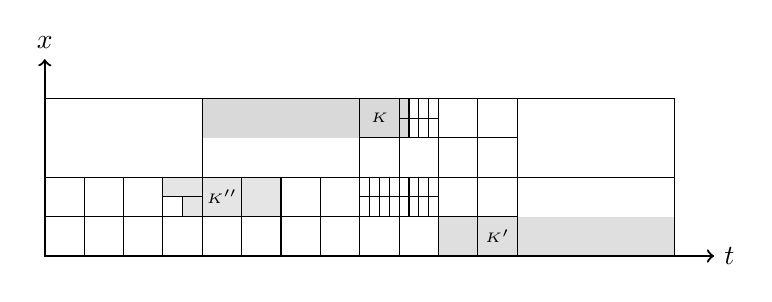
\begin{tikzpicture}
     \fill[gray!30] (2,1.5) rectangle (4.625,2); % Using gray!30 for light gray
     \fill[gray!25] (5,0.5) rectangle (8,0);
     \fill[gray!20] (1.75,0.5) rectangle (3,1);
     \fill[gray!20] (1.5,0.75) rectangle (2,1);
    % Draw the large rectangle
    \draw (0,0) rectangle (8,2); % Overall rectangle
    
    % Partition the rectangle into 2 rows
    \draw (0,1) -- (8,1); % Horizontal line for 2 rows
    
    % Partition the rectangles into 4 columns
    \draw (2,0) -- (2,2);
    \draw (4,0) -- (4,2);
    \draw (6,0) -- (6,2);
    
    % Bisect the 2nd and 3rd rectangle on the bottom row 3 times in x direction
    % This creates additional lines inside the 2nd and 3rd bottom rectangles
    %\draw (4,0) -- (4,1); % Middle line for 2nd rectangle, already exists
    
	\draw(.5,0) -- (.5,1); \draw(1,0) -- (1,1); \draw(1.5,0) -- (1.5,1);    
	\draw(1.5,0.75) -- (2.0,0.75);
    \draw(1.75,0.5) -- (1.75,.75);
    
	\draw (0,.5) -- (6,.5);
	\draw(2.5,0) -- (2.5,1); \draw(3,0) -- (3,1); \draw(3.5,0) -- (3.5,1);
	\draw(4.5,0) -- (4.5,1); \draw(5,0) -- (5,1); \draw(5.5,0) -- (5.5,1);
	\draw (4,1.5) -- (6,1.5);
	\draw(4.5,1) -- (4.5,2); \draw(5,1) -- (5,2); \draw(5.5,1) -- (5.5,2);
	\draw(4,.75) -- (5,.75);	
	\draw(4.25,.5) -- (4.25,1); \draw(4.125,.5) -- (4.125,1); \draw(4.375,.5) -- (4.375,1);
	\draw(4.75,.5) -- (4.75,1); \draw(4.625,.5) -- (4.625,1); \draw(4.875,.5) -- (4.875,1);
	
	\draw(4.5,1.75) -- (5,1.75);
	\draw(4.75,1.5) -- (4.75,2); \draw(4.625,1.5) -- (4.625,2); \draw(4.875,1.5) -- (4.875,2);
    
	\node at (4.25,1.75) {\tiny $K$};
	\node at (5.75,0.25) {\tiny $K'$};
	\node at (2.25,0.75) {\tiny $K''$};
    
    % Adding the axes
    % Draw x-axis
    \draw[->,thick] (0,0) -- (0,2.5) node[anchor=south] {$x$};
    % Draw t-axis
    \draw[->,thick] (0,0) -- (8.5,0) node[anchor=west] {$t$};
\end{tikzpicture}
\caption{A partition of a time-space cylinder with $d=1$, where the areas $q_K^t$, $q_{K'}^t$, and $q_{K''}^t$ for time-space cells $K,K',K''$ are marked gray. 
Notice that Assumption~\ref{ass:Partition}~\ref{itm:TimeSpaceCylNeighbors} does \emph{not} permit the area $q_{K''}^t$, since the left neighbors of $K''$ do not have the same time interval.}\label{fig:examplePartition}
\end{figure}
%
The grading assumption in \eqref{eq:EqualSizeNeighbors} allows for the following localization.
\begin{lemma}[Localized norm]\label{lem:localizedGeneral}
Each $v\in H^{1/2}(\mathcal{J};L^2(\Omega))$ satisfies 
\begin{equation}
\lvert v \rvert_{H^{1/2}(\cJ;L^2(\Omega))}^2 \lesssim \sum_{K\in \tria} \lvert v \rvert_{H^{1/2}(q_{K,t}^t;L^2(K_x))}^2 + h_{K,t}^{-1}\, \lVert v \rVert^2_{L^2(K)}.
\end{equation}
\end{lemma}
\begin{proof}
Let $v\in H^{1/2}(\mathcal{J};L^2(\Omega))$, and let $x \in \Omega$ with $\tria_t(x) \neq \emptyset$. Then $w \coloneqq v(\bigcdot,x)$ satisfies \cite[Lem.~4.2]{CarstensenFaermann01}
\begin{align*}
&\int_\mathcal{J} \int_\mathcal{J} \frac{|w(t)-w(s)|^2}{|t-s|^2} \dt\ds\\
&\qquad  \lesssim \sum_{K_t\in \tria_t(x)}  \int_{q_{K_t}(x)}  \int_{q_{K_t}(x)} \frac{|w(t)-w(s)|^2}{|t-s|^2} \dt\ds + |K_t|^{-1} \int_{K_t} |w(t)|^2 \dt.
\end{align*}
Integrating over all $x\in \Omega$ concludes the proof.
\end{proof}
\subsection{Finite element spaces}
Let $\tria$ be a partition of $Q$ satisfying Assumption~\ref{ass:Partition}.
For each time-space cylinder $K = K_t\times K_x\in \tria$ and all $p = (p_x,p_t)\in \mathbb{N}^2_0$ we set the polynomial spaces
\begin{align*}
\mathbb{P}_{p_t}(K_t) & \coloneqq \lbrace v_x \in L^2(K_t) \colon v_t \text{ is a polynomial of maximal degree }p_t\rbrace,\\
\mathbb{P}_{p_x}(K_x) & \coloneqq \lbrace v_x \in L^2(K_x) \colon v_x \text{ is a polynomial of maximal degree }p_x\rbrace,\\
\mathbb{P}_p(K) & \coloneqq \mathbb{P}_{p_t}(K_t) \otimes \mathbb{P}_{p_x}(K_x) \coloneqq \textup{span}\lbrace v_tv_x \colon v_t \in \mathbb{P}_{p_t}(K_t)\text{ and } v_x \in \mathbb{P}_{p_x}(K_t)\rbrace.
\end{align*}
Moreover, we set for all $p = (p_t,p_x)\in \mathbb{N}^2$ the space of piece-wise polynomial and globally continuous functions
\begin{align*}
W_h^{p_t,p_x} \coloneqq \lbrace v \in C^0(Q) \colon v|_K \in \mathbb{P}_p(K)\text{ for all }K\in \tria\rbrace.
\end{align*}
%
To include the homogeneous boundary data on $\mathcal{J} \times \partial \Omega$ we set 
\begin{equation}\label{eq:DefW_h0ptpx}
W_{h,0}^{p_t,p_x} \coloneqq W_h^{p_t,p_x} \cap W_0 \qquad\text{with } W_0 \coloneqq L^2(\mathcal{J} ;H^1_0(\Omega)) \cap H^{1/2}(\cJ;L^2(\Omega)).
\end{equation}
Our discrete trial space then reads with $p = (p_t,p_x) \in \mathbb{N}^2$
\begin{equation*}
U_h \coloneqq W_{h,0}^{p_t,p_x}.
\end{equation*}
%
The test space $V_h$ will be the sum of the lowest-order space 
\begin{equation*}
V_{h,0} \coloneqq W_{h,0}^{1,1} \cap V
\end{equation*}
and the span of suitable bubble functions defined as follows:

For all $K = K_t \times K_x \in \tria$ we set the non-negative bubble function
\begin{equation*}
\mathcal{B}_K \in \mathbb{P}_2(K_t) \otimes \mathbb{P}_{d+1}(K_x)\qquad\text{ with } \mathcal{B}_K|_{\partial K} = 0\text{ and } \lVert \mathcal{B}_K \rVert_{L^2(K)} = 1.
\end{equation*}
In other words, $\mathcal{B}_K$ is the scaled product of all local lowest-order basis functions associated to the vertices of $K$. We define the space of volume bubble functions as 
\begin{equation} \label{eq:volumebubble}
V_{h,2} \coloneqq \bigoplus_{K\in \tria} \mathcal{B}_K \big(\mathbb{P}_{p_t}(K_t) \otimes \mathbb{P}_{p_x-2}(K_x)\big) + \mathcal{B}_K \big(\mathbb{P}_{p_t-1}(K_t) \otimes \mathbb{P}_{p_x}(K_x)\big).
\end{equation}
%
Additionally, we define the following face bubble functions. 
Let $\mathcal{F}$ denote the set of all faces ($d$-hyperfaces of time-space cells) in $\tria$. 
We denote by $\mathcal{F}_t$ the set of all faces $f\in \mathcal{F}$ in $\tria$ that are orthogonal to the $\{0\} \times \Omega$ plane, and that do not contain children, that is,
\begin{equation*}
\mathcal{F}_t \coloneqq \lbrace f \in \mathcal{F} \colon f \perp \lbrace 0 \rbrace \times \mathbb{R}^d\text{ and any } g\in \mathcal{F}\text{ with } g \subset f \text{ satisfies }g =f  \rbrace.
\end{equation*}
The set $\mathcal{F}_{t,0} \subset \mathcal{F}_t$  denotes the set of all faces $f\in \mathcal{F}_t$ that are not on the lateral boundary, that is, $f\not \subset \overline{\cJ} \times \partial\Omega$.
We set for all faces $f \in \mathcal{F}_{t,0}$ the non-negative face bubble function
\begin{equation*}
\mathcal{B}_f \in W^{2,d}_h\qquad\text{with } \lVert \mathcal{B}_f \rVert_{L^2(Q)}=1\text{ and }\mathcal{B}_f|_g = 0\text{ for all }g\in \mathcal{F} \text{ with }g\not\subset f.
\end{equation*}
In other words, $\mathcal{B}_f$ is the scaled product of the local lowest-order basis functions associated to the vertices of $f$. Let $(\psi_j)_{j\in \mathcal{N}^{p_t,p_x-1}} \subset W^{p_t,p_x-1}_h$ denote the nodal basis with associated Lagrange nodes $\mathcal{N}^{p_t,p_x-1} \subset \overline{Q}$. Then we set the space of face bubble functions as 
\begin{equation} \label{eq:facebubble}
V_{h,1} \coloneqq \bigoplus_{f\in \mathcal{F}_{t,0}} \textup{span} \lbrace \mathcal{B}_f\, \psi_j \colon j \in \mathcal{N}^{p_t,p_x-1} \cap f  \rbrace.
\end{equation}
%
We finally set our discrete test space 
\begin{equation}\label{eq:testSpace}
V_h \coloneqq V_{h,0} \oplus V_{h,1} \oplus V_{h,2}.
\end{equation}
%
\begin{remark}[Optimal polynomial degrees] \label{rem:1} 
Let $\tria$ be a quasi-uniform triangulation with mesh sizes $h_x$ in space and $h_t$ in time. For smooth functions $u \in W_0$, the best approximation error $\min_{v_h\in W_{h,0}^{p_t,p_x}} \lVert u - v_h \rVert_W$, cf.~\eqref{eq:defNormW} below, is proportional to 
\begin{equation*}
\max\big\lbrace \max\lbrace h_t^{p_t+1},h_x^{p_x}\rbrace,\max \lbrace h_t^{p_t+1/2},h_x^{p_x+1}\rbrace \big\rbrace =\max \lbrace h_t^{p_t+1/2},h_x^{p_x}\rbrace.
\end{equation*}
Using the parabolic scaling $h_t=h_x^2$, both terms are equal when $2 p_t+1=p_x$. 
Since the same result is valid when $W_0$ is replaced by $L^2(\mathcal{J} ;H^1_0(\Omega)) \cap B^{1/2,p,2}(\mathcal{J};L^2(\Omega))$, Proposition~\ref{prop:2} shows that this result is also valid for the space $U$. Consequently, the choice $2 p_t+1=p_x$ of the  polynomial degrees $p=(p_t,p_x)$ for the discrete trial space $U_h$  is the most efficient one.
\end{remark}

\section{Interpolation and Fortin operator} \label{sec:Interpol}
The quasi-best approximation property \eqref{eq:QuasiBest} of our numerical scheme \eqref{eq:uhprime} requires the existence of a Fortin operator. We design such an operator in Section~\ref{subsec:Fortin}. A key tool in its design is a stable interpolation operator, which we analyze in the following Section~\ref{subsec:FEspaces}.
%
\subsection{Interpolation operator}\label{subsec:FEspaces}
We have shown in Lemma~\ref{lem:localizedGeneral} that the global norm of $v\in W$ is bounded from above by the sum of localized components. Equivalence does in general not hold. We will show, however, that local stable projectors $\mathcal{I} \colon L^2(\cJ;H^1(\Omega)) \to W_{h}^p$ with $p = (p_t,p_x) \in \mathbb{N}^2$ allow for a localization of the interpolation error.
We thereby focus on a Scott--Zhang operator similar to the original one in \cite{ScottZhang90}. Its definition involves the $L^2$ inner product $\langle \bigcdot ,\bigcdot \rangle_q \coloneqq \int_q \bigcdot \cdot \bigcdot \dx$ for volume contributions $q \subset \overline{Q}$ or boundary contributions $q\subset \overline{\mathcal{J}} \times \partial \Omega$.
%
\begin{definition}[Scott--Zhang operator]\label{def:SZ}
Let $p = (p_t,p_x) \in \mathbb{N}^2$ and let $(\psi_{j})_{j \in \mathcal{N}^p}$ denote the nodal basis of $W_h^p$ with corresponding Lagrange nodes $\mathcal{N}^p$. We assign to each nodal basis function $\psi_j$ with $j\not\in \overline{\cJ}\times \partial \Omega$ a time-space cylinder $S_j \in \tria$. If the Lagrange node of $\psi_\ell$ is on the lateral boundary $\overline{\cJ} \times \partial \Omega$, we choose $S_j \in \faces_t$ with $j\in S_j$ and define the bi-orthogonal basis function $\psi_j^* \in \mathbb{P}_{p}(S_j)$ such that
\begin{equation}\label{eq:DualWeight}
\langle \psi_\ell,\psi_j^*\rangle_{S_j} = \delta_{j,\ell}\qquad\text{for all }\ell \in \mathcal{N}^p(S_j),   
\end{equation}
where $\mathcal{N}^p(S_j)$ denotes the set of Lagrange nodes for $\mathbb{P}_{p}(S_j)$.
We set the operator 
\begin{equation}\label{eq:DefI}
\mathcal{I} \coloneqq \sum_{j\in \mathcal{N}^p} \langle \bigcdot ,\psi_{j}^*\rangle_{S_j} \psi_j.
\end{equation}
\end{definition}

Classical scaling arguments as for example in \cite{ScottZhang90,BrennerScott08} imply the following.
\begin{lemma}[Basic properties of $\mathcal{I}$] \label{lem:basicpropsSZ}
Any Scott--Zhang-type operator $\mathcal{I}$ defined as in Definition~\ref{def:SZ} 
\begin{itemize}
\item preserves homogeneous boundary data in the sense that $\mathcal{I}\colon W_0 \to W_{h,0}^p$,
\item satisfies the projection property $\mathcal{I} w_h = w_h$ for all $w_h \in W^p_h$,
\item is local in the sense that one has for all $K\in \tria$ the identity $(\mathcal{I} v)|_{K} = (\mathcal{I} w)|_{K}$ for all $v,w \in L^2(\cJ;H^1(\Omega))$ with $v|_{q_k} = w|_{q_k}$ and element patch 
\begin{equation*}
q_K \coloneqq \bigcup \lbrace \textup{supp}(\psi_j)\colon j \in \mathcal{N}^p\text{ and }K\subset \textup{supp}(\psi_j)\rbrace,
\end{equation*}
\item is locally  $L^2$ stable on $W_0$ in the sense that
\begin{equation}\label{eq:LocL2Stab}
\lVert \mathcal{I} w \rVert_{L^2(K)} \lesssim \lVert w \rVert_{L^2(q_K)}\qquad\text{for all }K\in \tria \text{ and }w\in W_{0}.
\end{equation}
\end{itemize}
\end{lemma}
Before we can verify the approximation properties of $\mathcal{I}$, we introduce the following version of \Poincare's inequality adapted to the spaces at hand.
Given a set $q \subset \mathbb{R}^m$ with $m\in \mathbb{N}$ and $m$-dimensional Lebesgue measure $|q|_m$, we define the integral mean of a function $g\colon q \to \mathbb{R}$ by
\begin{align*}
\langle g \rangle_q \coloneqq \dashint_q g \dx \coloneqq \frac{1}{|q|_m} \int_q g\dx.
\end{align*}

%
\begin{lemma}[Parabolic \Poincare{}]\label{lem:ParaPoincareH12}
Let $v\in L^2(K_t;H^1(K_x))\cap H^{1/2}(K_t;L^2(K_x))$ with time-space cylinder $K = K_t \times K_x$, where $K_t$ is an interval of length $h_t$ and $K_x \subset \mathbb{R}^d$ is some bounded domain with diameter $h_x$. We assume that $K_x$ allows for the \Poincare{} estimate $\lVert p - \langle p \rangle_{K_x}\rVert_{L^2(K_x)} \leq C_x h_x \lVert \nabla_x p \rVert_{L^2(K_x)}$ with constant $C_x < \infty$  for all $p\in H^1(K_x)$. Then we have
\begin{align*}
\lVert v - \langle v \rangle_K \rVert^2 _{L^2(K)}\leq C_x^2  h^2_x\, \lVert \nabla_x v \rVert^2_{L^2(K)} + h_t\, \lvert v \rvert^2_{H^{1/2}(K_t;L^2(K_x))}.
\end{align*}
\end{lemma}
\begin{proof}
Let $v\in L^2(K_t;H^1(K_x))\cap H^{1/2}(K_t;L^2(K_x))$ with time-space cylinder $K=K_t\times K_x$. The Pythagorean theorem and Fubini's theorem yield
\begin{align}\label{eq:Triangle1}
\lVert v - \langle v \rangle_K \rVert_{L^2(K)}^2 = \lVert v - \langle v \rangle_{K_x} \rVert_{L^2(K)}^2 
+ \lVert \langle v - \langle v \rangle_{K_t} \rangle_{K_x}\rVert^2_{L^2(K)}.
\end{align}
The first term is bounded due to \Poincare's inequality by 
\begin{align*}
\lVert v - \langle v \rangle_{K_x} \rVert^2_{L^2(K)} \leq C_x^2 h^2_x\, \lVert \nabla_x v \rVert_{L^2(K)}^2.
\end{align*}
Using Jensen's inequality for the squared second term in \eqref{eq:Triangle1} leads to 
\begin{align*}
 \lVert \langle v - \langle v \rangle_{K_t} \rangle_{K_x}\rVert^2_{L^2(K)} & = \int_K \Big|\dashint_{K_x} \dashint_{K_t} v(t,x) - v(s,x) \ds\dx\Big|^2 \mathrm{d}(t,y)\\
 & \leq \int_K  \dashint_{K_x} \dashint_{K_t} |v(t,x) - v(s,x)|^2 \ds\dx\, \mathrm{d}(t,y)\\
& = \int_{K_t} \dashint_{K_t} \lVert v(t) - v(s)\rVert_{L^2(K_x)}^2 \ds\dt\\
 &\leq h_t \int_{K_t} \int_{K_t} \frac{\lVert v(t) - v(s)\rVert_{L^2(K_x)}^2}{|t-s|^2} \ds\dt.
\end{align*}
Combining these results concludes the proof.
\end{proof}
Adaptively refined meshes require the use of the parabolic \Poincare{} inequality for non-cylindrical areas $q \subset \overline{Q}$. In our partitions these areas are build by unions of overlapping time-space cylinders $q_0,\dots,q_L$ with $L\in \mathbb{N}$ in the sense that
\begin{equation}\label{eq:decompQ}
q = \bigcup_{\ell=0}^L q_\ell\quad\text{and}\quad
|q_j| \eqsim \left|\bigcup_{\ell=0}^{j-1} q_\ell \cap q_{j}\right|\qquad \text{for all }j=1,\dots,L.
\end{equation} 
The generalized parabolic \Poincare{} inequality uses for all $v\in W$ with 
\begin{equation*}
W \coloneqq L^2(\cJ;H^1(\Omega)) \cap H^{1/2}(\cJ;L^2(\Omega))
\end{equation*}
 the semi-norm  
\begin{equation*}
\lvert v \rvert^2_{H^{1/2}L^2(q)} \coloneqq \int_\mathcal{J} \int_\mathcal{J} \int_\Omega \indicator_q(x,t) \indicator_q(x,s) \frac{|v(x,t) - v(x,s)|^2}{|t-s|^2} \dx \ds \dt.
\end{equation*}
\begin{lemma}[Generalized parabolic \Poincare{}]\label{lem:GenParaPoincareH12}
Suppose that $q \subset Q$ is some area covered by time-space cylinders $q_1,\dots,q_L$ as in \eqref{eq:decompQ}. Let $h_t$ and $h_x$ denote the diameters of $q$ in time and space direction, respectively.
Then we have for all $v\in W$ the parabolic \Poincare{} inequality
\begin{equation*}
\lVert v - \langle v \rangle_q \rVert^2_{L^2(q)} \lesssim  h_x^2 \, \lVert \nabla_x v \rVert_{L^2(q)}^2 + h_t\, \lvert v \rvert^2_{H^{1/2}L^2(q)}.
\end{equation*}
The hidden constant depends on $L$, the hidden constant in \eqref{eq:decompQ}, and the \Poincare{} constant in space $C_x$ for each time-space cylinder.
\end{lemma}
\begin{proof}
Let $v\in W$ and suppose $q \subset Q$ has a decomposition $q_0,\dots,q_L$ as in \eqref{eq:decompQ}. It holds, with $q^- \coloneqq  \bigcup_{\ell=0}^{L-1} q_\ell$, 
\begin{align*}
\lVert v - \langle v \rangle_q \rVert_{L^2(q)}^2 \leq  \lVert v - \langle v \rangle_{q^-} \rVert_{L^2(q)}^2 \leq \lVert v - \langle v \rangle_{q^-} \rVert_{L^2(q_L)}^2 + \lVert v - \langle v \rangle_{q^-} \rVert_{L^2(q^-)}^2.
\end{align*}
The first term satisfies 
\begin{align*}
\lVert v - \langle v \rangle_{q^-} \rVert_{L^2(q_L)}^2 = \lVert v - \langle v \rangle_{q_L} \rVert_{L^2(q_L)}^2 + \lVert \langle v \rangle_{q^-} - \langle v \rangle_{q_L} \rVert_{L^2(q_L)}^2.
\end{align*}
Jensen's inequality and \eqref{eq:decompQ} yield for the second addend, with $q^\textup{int}_L \coloneqq q^-\cap q_L$,
\begin{align*}
&\lVert \langle v \rangle_{q^-} - \langle v \rangle_{q_L} \rVert_{L^2(q_L)}^2 \leq 2 \, \lVert \langle v \rangle_{q^-} - \langle v \rangle_{q^\textup{int}_L} \rVert_{L^2(q_L)}^2+2\, \lVert \langle v \rangle_{q^\textup{int}_L} - \langle v \rangle_{q_L} \rVert_{L^2(q_L)}^2 \\
& \qquad = 2 \int_{q_L} \Big| \dashint_{q_L^\textup{int}} v  - \langle v \rangle_{q^-}\dy \Big|^2 \dz + 2 \int_{q_L} \Big| \dashint_{q_L^\textup{int}} v  - \langle v \rangle_{q_L}\dy \Big|^2 \dz \\
&\qquad \leq 2 \int_{q_L} \dashint_{q^\textup{int}_L} |v -\langle v \rangle_{q^-}|^2 \dy\dz + 2 \int_{q_L} \dashint_{q^\textup{int}_L} |v -\langle v \rangle_{q_L}|^2 \dy\dz\\
&\qquad = \frac{2\, |q_L|}{|q_L^\textup{int}|} \big( \lVert v -\langle v \rangle_{q^-} \rVert_{L^2(q^\textup{int}_L)}^2 + \lVert v -\langle v \rangle_{q_L} \rVert_{L^2(q_L)}^2\big)\\
&\qquad\leq \frac{2\, |q_L|}{|q_L^\textup{int}|} \big( \lVert v -\langle v \rangle_{q^-} \rVert_{L^2(q^-)}^2 + \lVert v -\langle v \rangle_{q_L} \rVert_{L^2(q_L)}^2\big).
\end{align*}
The contributions $\lVert v -\langle v \rangle_{q_L} \rVert_{L^2(q_L)}^2$ can be bounded by Lemma~\ref{lem:ParaPoincareH12}. We proceed inductively to bound the term $\lVert v -\langle v \rangle_{q^-} \rVert_{L^2(q^-)}$.
\end{proof}
\begin{remark}[Boundary]\label{rem:BoundaryPoincare}
Suppose that $q_L$ in \eqref{eq:decompQ} touches the lateral boundary of $Q$ in the sense that $q_L \cap \cJ \times \partial \Omega \neq \emptyset$. For any $v\in W_0$ one has the identity
\begin{align*}
\lVert v \rVert^2_{L^2(q)} = \lVert v - \langle v\rangle_q \rVert^2_{L^2(q)} + \lVert \langle v\rangle_q \rVert_{L^2(q)}^2.
\end{align*}
The first term can be bounded by Lemma~\ref{lem:GenParaPoincareH12}. Similar arguments as in the previous proof bound the second term by
\begin{align*}
\lVert \langle v\rangle_q \rVert_{L^2(q)} \leq \lVert \langle v\rangle_q - \langle v\rangle_{q_L^\textup{int}} \rVert_{L^2(q)} + \lVert \langle v\rangle_{q_L^\textup{int}} \rVert_{L^2(q)} \lesssim \lVert v - \langle v\rangle_q \rVert_{L^2(q)} + \lVert v \rVert_{L^2(q_L)}.
\end{align*}
Since \Poincare's inequality yields $\lVert v \rVert_{L^2(q_L)} \lesssim h_{K,x} \lVert \nabla_x v\rVert_{L^2(q_L)}$, we obtain
\begin{align*}
\lVert v  \rVert^2_{L^2(q)} \lesssim  h_x^2 \, \lVert \nabla_x v \rVert_{L^2(q)}^2 + h_t\, \lvert v \rvert^2_{H^{1/2}L^2(q)}.
\end{align*}
\end{remark}
%
Combining the properties of the Scott--Zhang operator with the parabolic \Poincare{} inequality leads to the following approximation result. 
%
\begin{lemma}[Local approximation property]\label{lem:locApx}
We have for all $K\in \tria$ 
and $w \in W_0$
\begin{align*}
\lVert w - \mathcal{I} w \rVert_{L^2(K)} &\lesssim h_{K,x} \lVert \nabla_x w \rVert_{L^2(q_K)} + h_{K,t}^{1/2}\, \lvert w \rvert_{H^{1/2}L^2(q_K)},\\
\lVert w - \mathcal{I} w \rVert_{L^2(K)} &\lesssim h_{K,x} \lVert \nabla_x (w - \mathcal{I} w) \rVert_{L^2(q_K)} + h_{K,t}^{1/2}\, \lvert w- \mathcal{I} w \rvert_{H^{1/2}L^2(q_K)}.
\end{align*}
\end{lemma}
\begin{proof}
Let $K\in \tria$ and $w \in W_0$.
By Assumption~\ref{ass:Partition} there exists a decomposition of $q = q_K$ into time-space cylinders $q_1,\dots,q_L$ as in \eqref{eq:decompQ}. If the patch $q_K$ touches the lateral boundary of $Q$ in the sense that $q_K \cap \cJ\times \partial \Omega \neq \emptyset$, Remark~\ref{rem:BoundaryPoincare} and the local $L^2$ stability of $\mathcal{I}$ for functions in $W_0$ yield
\begin{align*}
&\lVert w - \mathcal{I} w \rVert_{L^2(K)} \leq \lVert w \rVert_{L^2(K)} + \lVert \mathcal{I} w \rVert_{L^2(K)} \lesssim \lVert w \rVert_{L^2(q_K)}\\
&\qquad \lesssim h_{K,x} \lVert \nabla_x w \rVert_{L^2(q_K)} + h_{K,t}^{1/2} \lvert w\rvert_{H^{1/2}L^2(q_K)}.
\end{align*}
%
If $q_K \cap \cJ\times \partial \Omega = \emptyset$, the identity $\mathcal{I}1 = 1$, the triangle inequality, the local $L^2$ stability of $\mathcal{I}$ for functions in $W_0$, and Lemma~\ref{lem:GenParaPoincareH12} yield
\begin{align*}
&\lVert w - \mathcal{I} w \rVert_{L^2(K)} \leq \lVert w - \langle w \rangle_{q_K}\rVert_{L^2(K)} + \lVert \mathcal{I} (w-\langle w \rangle_{q_K})\rVert_{L^2(K)} \lesssim \lVert w-\langle w \rangle_{q_K} \rVert_{L^2(q_K)}\\
&\qquad \lesssim h_{K,x} \lVert \nabla_x w \rVert_{L^2(q_K)} + h_{K,t}^{1/2} \lvert w\rvert_{H^{1/2}L^2(q_K)}.
\end{align*}
This proves the first estimate.
 
The second estimate follows by the projection property allowing us to replace $w$ by $w-\mathcal{I} w$ in the first estimate of the lemma.
\end{proof}
%
Recall the definition of $q_K^t$ in \eqref{eq:def_qKt}.
Combining Lemma~\ref{lem:localizedGeneral} and \ref{lem:locApx} with the finite overlap of patches and the parabolic scaling yields the following localization of the norm in $W$ defined by
\begin{equation}\label{eq:defNormW}
\lVert \bigcdot \rVert_W \coloneqq (\lVert \nabla_x \bigcdot \rVert^2_{L^2(Q)} +  \lvert \bigcdot \rvert_{H^{1/2}(\cJ;L^2(\Omega))}^2)^{1/2}.
\end{equation}
\begin{theorem}[Localization of interpolation error]\label{thm:LocalizationIIold}
The interpolation error $\delta \coloneqq w - \mathcal{I}w$ with $w\in W_0$ localizes in the sense that 
\begin{align*}
\lVert \delta \rVert_W^2& \eqsim \sum_{K\in \tria}\lVert  \nabla_x \delta \rVert_{L^2(K)}^2 + \lvert  \delta \rvert_{H^{1/2}L^2(q^t_{K})}^2 + h_{K,t}^{-1} \lVert \delta \rVert_{L^2(K)}^2\\
& \eqsim \sum_{K\in \tria}\lVert  \nabla_x \delta \rVert_{L^2(K)}^2 + \lvert  \delta \rvert_{H^{1/2}L^2(q_K)}^2.
\end{align*}
\end{theorem}
In order to obtain local best-approximation properties of $\mathcal{I}$, we introduce the following inverse estimate.
\begin{lemma}[Inverse estimate]\label{lem:inverseEst}
For any $v_h \in W_h^p$ and $K\in \tria$ one has the inverse estimate, with hidden constant depending only on the polynomial degree $p_t$ and the equivalence constants in \eqref{eq:EqualSizeNeighbors}, 
\begin{equation*}
\lvert v_h \rvert_{H^{1/2}L^2(q_{K}^t)} \lesssim h_{K,t}^{-1/2}\, \lVert v_h\rVert_{L^2(q_K^t)}.
\end{equation*}  
\end{lemma}
\begin{proof}
Let $v_h \in W_h^p$ and let $x\in K_x$ with $K=K_t\times K_x\in \tria$. The function $v_h(\bigcdot,x)$ is a piece-wise polynomial with respect to the quasi-uniform (see~\eqref{eq:EqualSizeNeighbors}) underlying partition $\lbrace K_{t,1},K_{t,2},K_{t,3} \rbrace$ of $q_{K_t}(x)$. Scaling arguments yield
\begin{align*}
\lvert v_h(\bigcdot,x) \rvert_{H^{1/2}(q_{K_t}(x))}^2 &= \sum_{j = 1}^3 \sum_{k=1}^3 \int_{K_{t,j}} \int_{K_{t,k}} \frac{|v_h(t,x) -v_h(s,x) |^2}{|t-s|^2} \dt \ds \\
&\lesssim h_{K,t}^{-1} \, \lVert v_h(\bigcdot,x)  \rVert_{L^2(q_{K_t}(x))}^2.
\end{align*}
Integrating over all $x\in K_x$ concludes the proof.
\end{proof}
%
With the inverse estimate and the local $L^2$-stability of $\mathcal{I}$ we can bound the addends of the localized interpolation error by best-approximations as shown in the following lemma. The result involves the extended patch 
\begin{equation*}
q(q_K^t) \coloneqq \bigcup \lbrace q_{K'} \colon K'\in \tria\text{ with }\textup{int}(K') \cap q_K^t \neq \emptyset\rbrace.
\end{equation*}
\begin{lemma}[Local quasi-optimality]\label{lem:LocalQuasiOpt}
The interpolation error $\delta \coloneqq w - \mathcal{I} w$ with $w\in W_0$ satisfies on each $K\in \tria$ the local quasi-optimality result
\begin{align*}
&\lVert  \nabla_x \delta \rVert_{L^2(K)}^2 + \lvert  \delta \rvert_{H^{1/2}L^2(q^t_K))}^2 + h_{K,t}^{-1} \lVert \delta \rVert_{L^2(K)}^2 \\
& \qquad\quad  \lesssim \min_{w_h \in W^p_{h,0}} \lVert  \nabla_x (w-w_h) \rVert_{L^2(q(q_K^t))}^2 + \lvert w - w_h \rvert^2_{H^{1/2}L^2(q(q_K^t))}.
\end{align*}
\end{lemma}
\begin{proof}
Let $w \in W_0$ and $K\in \tria$. We focus on deriving an upper bound for the term $\lvert  \delta \rvert_{H^{1/2}L^2(q^t_K)}^2$. The remaining bounds follow similarly. The triangle inequality and the projection property of $\mathcal{I}$ yield for all $w_h \in W_{h,0}^p$
\begin{equation*}
\lvert \delta \rvert_{H^{1/2}L^2(q^t_K)} \leq  \lvert w- w_h \rvert_{H^{1/2}L^2(q^t_K)} + \lvert \mathcal{I}(w-w_h) \rvert_{H^{1/2}L^2(q^t_K)}.
\end{equation*}
The inverse estimate in Lemma~\ref{lem:inverseEst}, the local $L^2$-stability of $\mathcal{I}$ from Lemma~\ref{lem:basicpropsSZ} for functions in $W_0$, and the parabolic \Poincare{} inequality in Lemma~\ref{lem:GenParaPoincareH12} lead to
\begin{align*}
\lvert \mathcal{I}(w-w_h) \rvert_{H^{1/2}L^2(q^t_K)} & = \lvert \mathcal{I}(w-w_h - \langle w - w_h\rangle_{q(q_K^t)}) \rvert_{H^{1/2}L^2(q^t_K)}\\
& \lesssim h_{t,K}^{-1/2}\lVert  w - w_h - \langle w - w_h\rangle_{q(q_K^t)} \rVert_{L^2(q(q_K^t))} \\
& \lesssim \lVert \nabla_x (w-w_h) \rVert_{L^2(q(q_K^t))} + \lvert w - w_h \rvert_{H^{1/2}L^2(q(q_K^t))}.\qedhere
\end{align*}
\end{proof}
%
Combining Theorem~\ref{thm:LocalizationIIold} and Lemma~\ref{lem:LocalQuasiOpt} yields the following corollary.
\begin{corollary}[Local best-approximation]\label{cor:QuasBest}
One has for all $w\in W_0$
\begin{align*}
\lVert w-\mathcal{I} w \rVert_W^2
 \eqsim \sum_{K\in \tria} \min_{w_h\in W^p_{h,0}} \lVert  \nabla_x (w-w_h) \rVert_{L^2(q(q^t_K))}^2 + \lvert w-w_h \rvert_{H^{1/2}L^2(q(q^t_K))}^2.
\end{align*} 
\end{corollary}
%
By taking $w_h=0$ in the corollary and using the finite overlap of patches, we obtain the following stability result.
\begin{corollary}[Stability]\label{cor:Stability}
The operator $\mathcal{I}\colon W_0 \to W_{h,0}^p$ is uniformly stable with respect to the norm in $W$ in the sense that 
\begin{align*}
\|\mathcal{I} u\|_W^2+ \sum_{K \in \tria} h_{K,x}^{-2} \, \|(1-\mathcal{I})u\|^2_{L^2(K)} \lesssim \|u\|_W^2.
\end{align*}
\end{corollary}
%
We conclude this subsection with a modification of $\mathcal{I}$ mapping into discretizations of $U_F$ or $V_F$ defined in \eqref{eq:DefUvV}.
\begin{remark}[Zero initial or end data]\label{rem:IforUandV}
Let $V_h \coloneqq  W^p_{h,0} \cap V_F$. Then we extend the partition $\tria$ to a partition of the half space $(0,\infty) \times \Omega$ by mirroring the partition at times $T, 2T,\dots$ . We now define the operator $\mathcal{I}$ on these partitions as in Definition~\ref{def:SZ} of the half space such that degrees of freedom $\psi_\ell$ with Lagrange node at time $T$ use dual basis functions $\psi_\ell^*$ supported outside of $Q$. The resulting operator $\mathcal{I}$ maps $V_F$ onto $V_h$ and has the localization property displayed in Theorem~\ref{thm:LocalizationIIold}, where the left-hand side involves the $H^{1/2}((0,\infty);H)$ norm that is equivalent to the $H^{1/2}_{,0}(\cJ;H)$ norm as discussed in Remark~\ref{rem:ExtByZero}.
This allows us to replace the norm $\lVert \bigcdot \rVert_W$ in Lemma~\ref{lem:LocalQuasiOpt} as well as Corollary~\ref{cor:QuasBest} and \ref{cor:Stability} by the norm $\lVert \bigcdot \rVert_V$.
Similar modifications lead to an interpolation operator $\mathcal{I} \colon U_F \to W^p_{h,0}\cap U_F$.
\end{remark}
%
\subsection{Fortin operator}\label{subsec:Fortin}
%
In this subsection we extend the design of the interpolation operator in Section~\ref{subsec:FEspaces} to ensure the existence of a bounded operator $F\colon V \to V_h \subset V$ that satisfies, with trial space $U_h \coloneqq W_{h,0}^p$ and polynomial degree $p = (p_t,p_x)\in \mathbb{N}^2$, the annihilation property
\begin{equation*}
b(u_h,v-F v) = 0\qquad\text{for all }u_h \in U_h\text{ and }v\in V.
\end{equation*}
It is known that the existence of such a so-called Fortin operator yields the injectivity of the discretized operator equation $B\colon U_h \to V_h'$ \cite{Fortin77} and leads to quasi-optimality in suitable minimal residual methods \cite[Thm.~3.6]{MonsuurStevensonStorn23}. 

\begin{theorem}[Fortin operator]\label{thm:FortinOperator}
There exists a continuous linear operator $F\colon V \to V_h$ with the annihilation property
\begin{equation*}
b(u_h,v - F v) = 0\qquad\text{for all }u_h\in U_h\text{ and }v\in V.
\end{equation*}
\end{theorem}
\begin{proof}
\textit{Step 1 (Definition of the operator).}
From \eqref{eq:volumebubble} and  \eqref{eq:facebubble}, recall the definition of the bubble spaces $V_{h,1}$ and $V_{h,2}$.
We define the correction operator $\mathcal{C}_1 \colon V \to V_{h,1}$, which is according to the definition of $V_{h,1}$ uniquely characterized by its values on the faces $f\in \mathcal{F}_{t,0}$, such that
\begin{equation}\label{eq:DefC1}
\int_f \xi (v- \mathcal{C}_1 v)\ds = 0 \quad\text{for all }v\in V, f\in \mathcal{F}_{t,0}, \xi \in \mathbb{P}_{p_t}(f_t)\otimes \mathbb{P}_{p_x-1}(f_x).
\end{equation}
%
Moreover, we set the correction operator $\mathcal{C}_2 \colon V \to V_{h,2}$ such that for all $v\in V$, $K\in \tria$, and $\theta \in \mathbb{P}_{p_t}(K_t) \otimes \mathbb{P}_{p_x-2}(K_x) + \mathbb{P}_{p_t-1}(K_t) \otimes \mathbb{P}_{p_x}(K_x)$
\begin{equation}\label{eq:DefC2}
\int_K \theta (v-\mathcal{C}_2 v) \dx = 0.
\end{equation}
%
Let $\mathcal{I} \colon V \to V_{h,0}$ be the interpolation operator discussed in Section~\ref{subsec:FEspaces} with the modification in Remark~\ref{rem:IforUandV}.
We define for all $v\in V$ the composed mapping
\begin{align*}
F v \coloneqq \mathcal{I} v - \mathcal{C}_1 \delta - \mathcal{C}_2 ( \delta - \mathcal{C}_1 \delta )\qquad\text{with }\delta \coloneqq v - \mathcal{I} v.
\end{align*}

\textit{Step 2 (Annihilation property of $F$).}
Let $u_h \in U_h$ and $v \in V$.
We set $\delta \coloneqq v - \mathcal{I} v$. An element-wise integration by parts reveals
\begin{align*}
&b(u_h,v-Fv) = b(u_h,\delta -\mathcal{C}_1 \delta - \mathcal{C}_2 ( \delta - \mathcal{C}_1 \delta ))\\
&\quad = \sum_{K\in\tria} \langle \partial_t u_h-\Delta_x u_h ,(1- \mathcal{C}_2)(\delta - \mathcal{C}_1 \delta)\rangle_K + \int_{K_t} \int_{\partial K_x} \nabla_x u_h \cdot \nu_x\,  (1 - \mathcal{C}_1 ) \delta\dx \ds.
\end{align*}
The volume contributions equal zero due to \eqref{eq:DefC2} and the integral over the faces equals zero due to \eqref{eq:DefC1}.

\textit{Step 3 (Boundedness of $F$).}
Let $\widehat{F}:= \mathcal{I} + \mathcal{C}_1(1-\mathcal{I})$, so that $F:= \widehat{F} + \mathcal{C}_2(1-\widehat{F})$.
We show that for $G \in \{\mathcal{I}, \widehat{F}, F\}$, 
\be \label{eq:G}
\|G v\|_V^2+ \sum_{K \in \tria} h_{K,x}^{-2}\, \|(1-G)v\|^2_{L^2(K)} \lesssim \|v\|_V^2.
\ee
This yields in particular $\|F u\|_V \lesssim \|u\|_V$.

For $G=\mathcal{I}$, Corollary~\ref{cor:Stability} and Remark~\ref{rem:ExtByZero} yield the claim in \eqref{eq:G}.
%
The parabolic scaling assumption in \eqref{eq:ParabolicScaling}, the inverse inequalities in Lemma~\ref{lem:localizedGeneral} and \ref{lem:inverseEst}, and the trace inequality $\|v\|^2_{L^2(f)} \lesssim h_{K,x}^{-1}\|v\|_{L^2(K)}^2+h_{K,x}\|v\|_{L^2(K_t;H^1(K_x))}^2$ for $f \in \mathcal{F}_t$ with $f \subset K \in \tria$ yield
\begin{equation} \label{eq:temp}
\begin{split}
\|  \mathcal{C}_1 v\|_V^2 \lesssim \sum_{K \in \tria} h_{K,x}^{-2}\, \|\mathcal{C}_1 v\|^2_{L^2(K)} &\lesssim \|v\|^2_{L^2(\mathcal{J};H^1_0(\Omega))}+\sum_{K \in \tria} h_{K,x}^{-2}\, \| v\|^2_{L^2(K)} \\
& \lesssim \|v\|^2_{V}+\sum_{K \in \tria} h_{K,x}^{-2}\, \| v\|^2_{L^2(K)}.
\end{split}
\end{equation}
%
Hence, the definition of $\widehat{F}$ and the already stated result for $\mathcal{I}$ verify \eqref{eq:G} for $G=\widehat{F}$. 
Similarly, we conclude \eqref{eq:G} for $G=F$ from
\begin{equation*}
\|  \mathcal{C}_2 u\|_V^2 \lesssim \sum_{K \in \tria} h_{K,x}^{-2} \|\mathcal{C}_2 u\|^2_{L^2(K)} \lesssim \sum_{K \in \tria} h_{K,x}^{-2} \| u\|^2_{L^2(K)}.
\end{equation*}
%
This shows that the linear operator $F\colon V \to V_h$ is continuous.
\end{proof}
%
The existence of the Fortin operator ensures the quasi-optimality of the numerical scheme discussed in the following section. The price to be paid is the parabolic scaling, which is more natural for the parabolic problem but leads to  more degrees of freedom than needed for smooth problems. We counter this effect by using different polynomial degrees in space and time as discussed in Remark~\ref{rem:1}.
%
%
\section{Preconditioner}\label{sec:preCond}
As explained in Section~\ref{subsec:discreteSetting}, we have to replace the inner product $\langle \bigcdot , \bigcdot \rangle_V$ in \eqref{eq:SaddlePointProb} by a suitable inner product $(G_h^{-1}\bigcdot)(\bigcdot)$ on $V_h\times V_h$ with induced norm being uniformly equivalent to the norm $\lVert \bigcdot \rVert_V$. The operator $G_h\in \cL(V_h', V_h)$ is a preconditioner that we will introduce in the following two subsections. A key tool in our design and analysis of $G_h$ is the following classical result, cf.~\cite[Sec.~4.1]{Oswald94}.
\begin{theorem}[Additive subspace correction] \label{thm:1}
Let $\U$ be a Hilbert space, and let $(\U_i)_i$ be a family of Hilbert spaces with embeddings $ E_i\colon \U_i \rightarrow \U$ such that
\begin{equation*}
\bigcup_i E_i(\U_i)=\U.
\end{equation*}
We set
\begin{equation*}
\lnrm u\rnrm_\U^2 \coloneqq \inf_{\{(u_i)_{i} \in \prod_{i} \U_i\colon \sum_{i} E_i u_i=u\}} \textstyle{\sum_{i}} \|u_i\|^2_{\U_i}\qquad\text{for all }u\in \U.
\end{equation*}
Let $R_i\colon \U_i' \rightarrow \U_i$ be the Riesz isomorphism. Then
$G \coloneqq \sum_{i} E_i R_i E_i'\in \Lis(\U',\U)$ is a linear isomorphism with
\begin{equation*}
\inf_{0 \neq u \in \U} \frac{\nrm u\nrm_\U}{\|u\|_\U} \leq
\frac{(G^{-1}\bigcdot)(\bigcdot)^{1/2}}{\|\bigcdot\|_{\U}} \leq
\sup_{0 \neq u \in \U} \frac{\nrm u\nrm_\U}{\|u\|_\U} \qquad\text{on } \U\setminus \{0\}.
\end{equation*}
\end{theorem}
%\begin{proof}
%A proof can for example be found in \cite[Sect.~4.1]{Oswald94}.
%\end{proof} 
%
\subsection{Splitting and bubbles}\label{subsec:Splitting}
Due to the addition of edge bubbles for the construction of our Fortin interpolator, the test spaces $V_h \coloneqq V_{h,0} \oplus V_{h,1} \oplus V_{h,2}$ defined in \eqref{eq:testSpace} are not nested under mesh refinement. Therefore, we decompose the test space into the space without bubbles $V_{h,0}$ and the bubble part $\mathcal{B}_h\coloneqq  V_{h,1} \oplus V_{h,2}$. This splitting will be stable with respect to the $\|\bigcdot\|_V$-norm, allowing us to precondition both parts separately. 
As we will see, on the bubble-part a diagonal preconditioner will suffice. 
The following proposition summarizes these ideas.

\begin{proposition}[Splitting]\label{prop:splitting} Let $V_h=V_{h,0} \oplus \mathcal{B}_h$ such that
\be \label{eq:7}
\|v+b\|_V^2 \eqsim \|v\|_V^2+ \|b\|_V^2 \qquad\text{for all }v \in V_{h,0},\,b \in \mathcal{B}_h.
\ee
Let $G_{h,0}\colon V_{h,0} ' \rightarrow V_{h,0}$ be such that
\be \label{eq:8}
\|\bigcdot\|_V^2 \eqsim (G_{h,0}^{-1}\,\bigcdot)(\bigcdot) \quad \text{on } V_{h,0}.
\ee
Let $\Psi_h$ be a basis for $\mathcal{B}_h$ such that one has for all scalars $c_\psi$ the equivalence
\be \label{eq:9}
\Big\|\sum_{\psi \in \Psi_h} c_\psi \psi\Big\|_V^2 \eqsim \sum_{\psi \in \Psi_h} c_\psi^2.
\ee
%
Then with $G_{h,1}\colon \mathcal{B}_h'\rightarrow \mathcal{B}_h$ defined by $G_{h,1}f :=\sum_{\psi \in \Psi_h} f(\psi)\psi$, and 
with the inclusions $E_{h,0}\colon V_{h,0} \rightarrow V_h$ and $E_{h,1}\colon \mathcal{B}_h \rightarrow V_h$ the operator
\begin{equation}\label{eq:SplittedPrecond}
G_h\coloneqq E_{h,0} G_{h,0} E_{h,0}'+ E_{h,1} G_{h,1} E_{h,1}'\colon V_h' \rightarrow V_h
\end{equation}
satisfies 
\begin{equation*}
\|\bigcdot\|_V^2 \eqsim (G_h^{-1}\bigcdot)(\bigcdot) \quad \text{on } V_h.
\end{equation*}
\end{proposition}

\begin{proof} For $V_{h,0}$ equipped with scalar product $(G_{h,0}^{-1} \,\bigcdot)(\bigcdot)$, the Riesz isomorphism $V_{h,0}'\rightarrow V_{h,0}$ is $G_{h,0}$.
For $\mathcal{B}_h$ equipped with scalar product 
\begin{equation*}
\Big(\sum_{\psi \in \Psi} c_\psi \psi,\sum_{\phi \in \Psi} d_\phi \phi\Big) \mapsto 
\sum_{\psi \in \Psi} c_\psi d_\phi,
%\langle \vec{c},\vec{d} \rangle,
\end{equation*}
the Riesz isomorphism $\mathcal{B}_h'\rightarrow \mathcal{B}_h$ is $G_{h,1}$. Now the result follows from Theorem~\ref{thm:1}, where the (uniform) equivalence of the triple-bar norm with $\|\bigcdot\|_V$ on $V_h$ follows from the assumptions in \eqref{eq:7}--\eqref{eq:9}.
\end{proof}
%
The following lemma verifies the assumptions of Proposition~\ref{prop:splitting}.
\begin{lemma}[Verification of assumptions]
The spaces $V_{h,0}$ and $\mathcal{B}_h \coloneqq V_{h,1} \oplus V_{h,2}$ defined in \eqref{eq:testSpace} satisfy the assumptions in \eqref{eq:7} and \eqref{eq:9} with $\Psi_h$ consisting of scaled Lagrange basis functions.
\end{lemma}
\begin{proof}

Let $(\psi_j)_{j=1}^N$ denote the nodal basis of $V_{h,0}$ and let $(\psi_j)_{j=N+1}^M $ denote a local basis of $\mathcal{B}_h$ that is $L^2(Q)$-normalized, i.e.~$\lVert \psi_j \rVert_{L^2(Q)}=1$ for all $j=N+1,\dots,M$.
We define the Scott--Zhang interpolation operator $\overline{\mathcal{I}}\colon W \to V_h$ as in Definition~\ref{def:SZ}, that is, with suitable bi-orthogonal weights $(\psi_j^*)_{j=1}^{N+M}$ the operator reads 
\begin{equation*}
\overline{\mathcal{I}} \coloneqq \sum_{j=1}^{N+M} \langle \psi_j^*,\bigcdot \rangle_{S_j} \psi_j.
\end{equation*}
Moreover, we set its reduced version $\mathcal{I}\colon W \to V_{h,0}$ as
\begin{equation*}
\mathcal{I} \coloneqq \sum_{j=1}^N \langle \psi_j^*,\bigcdot \rangle_{S_j} \psi_j.
\end{equation*}
Let $v\in V_{h,0}$ and $b \in \mathcal{B}_h$.
By definition we obtain $\mathcal{I} b = 0$. 
This identity and the stability properties of $\mathcal{I}$ stated in Corollary~\ref{cor:Stability} yield
\begin{equation*}
\lVert v \rVert_V + \lVert b \rVert_V = \lVert \mathcal{I} (v + b) \rVert_V + \lVert (1-\mathcal{I}) (v + b) \rVert_V  \lesssim \lVert v+b\rVert_V.
\end{equation*}
This verifies \eqref{eq:7}.


Theorem~\ref{thm:LocalizationIIold}, Lemma~\ref{lem:inverseEst}, and Lemma~\ref{lem:locApx} yield the norm equivalence
\begin{equation}\label{eq:NormEquiB}
\begin{aligned}
\|b\|_V^2 & = \|(1-\mathcal{I}) b\|_V^2  \lesssim \sum_{K \in \tria} h_{K,t}^{-1}\, \|b\|_{L^2(K)}^2 = \sum_{K \in \tria} h_{K,t}^{-1}\, \| (1-\mathcal{I})b\|_{L^2(K)}^2 \\
& \lesssim \|b\|_V^2.
\end{aligned}
\end{equation}
Since the number $\#\{ j \in \lbrace N+1,\dots,M\rbrace\colon |\supp \psi_j \cap K|>0\} \eqsim 1$ of bubble basis functions supported on each $K\in \tria$ is uniformly bounded, we obtain for any $b\in \mathcal{B}_h$ with representation $b = \sum_{j=N+1}^M c_j \psi_j$ and $K\in \tria$ the equivalence
\begin{equation*}
\Big\|\sum_{\substack{j = N+1 ,\dots,M \\ |\supp \psi_j \cap K|>0}} c_j \psi_j\Big\|_{L^2(K)} ^2\eqsim \sum_{\substack{j = N+1 ,\dots,M \\ |\supp \psi_j \cap K|>0}} c_j^2\, \| \psi_j\|_{L^2(K)}^2.
\end{equation*}
This bound, \eqref{eq:NormEquiB}, and the mesh properties stated in Assumption~\ref{ass:Partition}  verify \eqref{eq:9} with basis 
\begin{equation*}
\Psi_h = \big(\textup{diam}_x(\supp(\psi_j))  \, \psi_j\big)_{j=N+1}^M.\qedhere
\end{equation*}
\end{proof}



\subsection{Additive subspace correction}\label{subsec:AddSubspaceCorr}
In this section we design a preconditioner $G_{h,0}= G_L\colon V_L'\to V_L$ with $V_L \coloneqq W_{h,0}^p \subset V$ with the property \eqref{eq:8}. 
In view of a later construction of a preconditioner at the trial side, we consider the more general situation of arbitrary polynomial degrees $p = (p_t,p_x)\in \mathbb{N}^2$. 
In order to design $G_L$, we generalize the fractional spaces defined in \eqref{eq:InterpolSpaceTime}, that is, we set for any $s \in [0,1]$ the interpolation spaces
\begin{align*}
&\cH^{2s}(\Omega)\coloneqq [H^1_0(\Omega) \cap H^2(\Omega),L^2(\Omega)]_{1-s,2},\quad
\cH^s(\cJ)\coloneqq [H^1_{,0}(\cJ),L^2(\cJ)]_{1-s,2},\\
&\cH^{2s,s}(Q)\coloneqq [L^2(\cJ;\cH^2(\Omega)) \cap \cH^1(\cJ;L^2(\Omega)),L^2(Q)]_{1-s,2}.
\end{align*}
In particular, we obtain the isomorphisms
\begin{align*}
\cH^{1,1/2}(Q)& \simeq L^2(\cJ;\cH^{1}(\Omega)) \cap \cH^{1/2}(\cJ;L^2(\Omega))\\
& \simeq L^2(\cJ;H^1_0(\Omega)) \cap H^{1/2}_{,0}(\cJ;L^2(\Omega)) = V.
\end{align*}

The operator $G_L$ will be of multi-level type. We start our design with collecting some ingredients for the \emph{uniform refinement case}.
Recall our initial partition $\tria_0 = \tria_t \otimes \tria_x$ of $Q$ and refinement strategy discussed in Section~\ref{subsec:tria}. Uniform refinements lead to a nested sequence of conforming partitions 
\begin{equation*}
\tria_0 = \widehat{\tria}_0 < \widehat{\tria}_1 < \widehat{\tria}_2 < \cdots .
\end{equation*}
Each prism $K=K_t \times K_x \in \widehat{\tria}_\ell$ with $\ell\in \mathbb{N}_0$ consists of a time interval $K_t$ with $\diam(K_t) = |K_t| \eqsim \varrho^{-2\ell}$ and a uniformly shape regular $d$-simplex $K_x$ with $\diam( K_x)\eqsim \varrho^{-\ell}$ with constant $\varrho = 2$. 
For each uniform refinement $\widehat{\tria}_\ell$, $\ell \in \mathbb{N}_0$, the corresponding finite element spaces read
\begin{equation*}
\widehat{V}_\ell \coloneqq \{v \in \cH^{1,1/2}(Q)\colon v|_{K_t \times K_x} \in \P_{p_t}(K_t) \otimes \P_{p_x}(K_x) \text{ for all }K \in \widehat{\tria}_\ell\} \subset V.
\end{equation*}
Classical approximation results verify the Jackson estimate
\begin{equation}\label{eq:Jackson}
\min_{w \in \widehat{V}_\ell}\|u-w\|_{L^2(Q)} \lesssim \varrho^{-2\ell} \|u\|_{\cH^{2,1}(Q)}\qquad \text{for all }u \in \cH^{2,1}(Q).
\end{equation}
Writing $\widehat{V}_\ell = \widehat{V}_{\ell,t} \otimes \widehat{V}_{\ell,x}$, for $s \in \{0,1\}$, and thus by interpolation for all $s \in [0,1]$, we have $\|\bigcdot\|_{\cH^{s}(\cJ)} \lesssim \varrho^{2\ell s}\|\bigcdot\|_{L^2(\cJ)}$ on $\widehat{V}_{\ell,t}  $, and so $\|\bigcdot\|_{\cH^{s}(\cJ;L^2(\Omega))} \lesssim \varrho^{2\ell s}\|\bigcdot\|_{L^2(Q)}$ on $\widehat{V}_{\ell} $. For $s<3/4$, we have $\|\bigcdot\|_{\cH^{2s}(\Omega)} \lesssim \varrho^{2\ell s}\|\bigcdot\|_{L^2(\Omega)}$ on $\widehat{V}_{\ell,x}$ \cite{75.64}, and so 
$\|\bigcdot\|_{L^2(\cJ;\cH^{2s}(\Omega))} \lesssim \varrho^{2\ell s}\|\bigcdot\|_{L^2(Q)}$ on $\widehat{V}_{\ell}$. Since $\cH^{2s,s}(Q) \simeq L^2(\cJ;\cH^{2s}(\Omega)) \cap \cH^{s}(\cJ;L^2(\Omega))$, these bounds yield for any $\gamma \in [0,3/4)$ the Bernstein estimate
\begin{equation}\label{eq:Bernstein}
 \|w\|_{\cH^{2\gamma,\gamma}(Q)} \lesssim \varrho^{2 \ell \gamma} \|w\|_{L^2(Q)} \qquad \text{for all }w \in \widehat{V}_\ell. 
\end{equation}

As a consequence of \eqref{eq:Jackson}--\eqref{eq:Bernstein}, and the nesting $\widehat{V}_\ell \subset \widehat{V}_{\ell+1}$, we have the following result involving the $L^2(Q)$-orthogonal projector onto $\widehat{V}_i$ denoted by
\begin{equation*}
P_\ell \colon L^2(Q) \to \widehat{V}_\ell\qquad\text{with } P_{-1}\coloneqq 0.
\end{equation*}
%
\begin{theorem}[Norm equivalence I]\label{thm:NormEqui}
 One has for $s \in (-\frac34,\frac34)$ the equivalence
\begin{equation*}
\|u\|^2_{\cH^{2s,s}(Q)} \eqsim \sum_{\ell=0}^\infty \varrho^{4s\ell}\|(P_\ell -P_{\ell-1})u\|_{L^2(Q)}^2 \qquad \text{for all }u \in \cH^{2s,s}(Q),
\end{equation*}
where $\cH^{2s,s}(Q)\coloneqq \cH^{-2s,-s}(Q)'$ for $s<0$.
\end{theorem}
\begin{proof}
This result is shown in \cite[Thm.~2.1]{DahmenStevenson99}.
\end{proof}
\begin{corollary}[Norm equivalence II] \label{corol:1} One has for all $s \in (0,\frac34)$ and $u \in \cH^{2s,s}(Q)$
\begin{equation*}
\sum_{\ell=0}^\infty \varrho^{4s\ell}\|(\identity - P_\ell)u\|_{L^2(Q)}^2 + \lVert P_0 u \rVert_{L^2(Q)}^2 \eqsim \|u\|^2_{\cH^{2s,s}(Q)}.
\end{equation*}
\end{corollary}
\begin{proof}
Any $u\in \cH^{2s,s}(Q)$ satisfies due to Theorem~\ref{thm:NormEqui}
\begin{align*}
&\sum_{\ell=0}^\infty \varrho^{4s\ell}\|(\identity - P_\ell)u\|_{L^2(Q)}^2
=\sum_{\ell=0}^\infty \varrho^{4s\ell}\sum_{j=0}^\infty \|(P_j-P_{j-1})(\identity - P_\ell)u\|_{L^2(Q)}^2
\\
&=\sum_{\ell=0}^\infty \varrho^{4s\ell} \sum_{j > \ell} \|(P_{j+1} - P_{j})u\|_{L^2(Q)}^2
\\
&=\sum_{j=1}^\infty \Big(\sum_{\ell=0}^{j-1} \varrho^{4s(\ell-j-1)} \Big)\varrho^{4s(j+1)}  \|(P_{j+1} - P_j)u\|_{L^2(Q)}^2\\
&\leq \tfrac{1}{1-\varrho^{-4 s}}\sum_{j=1}^\infty \varrho^{4s(j+1)}  \|(P_{j+1} - P_j)u\|_{L^2(Q)}^2\lesssim  \|u\|^2_{\cH^{2s,s}(Q)}.
\end{align*}
Combining this estimate with  $\lVert P_0 u \rVert_{L^2(Q)}^2\leq \lVert u \rVert_{L^2(Q)}^2 \lesssim \|u\|^2_{\cH^{2s,s}(Q)}$ yields the lower bound.
%
The upper bound follows from
\begin{align*}
\|u\|^2_{\cH^{2s,s}(Q)} &\eqsim \sum_{\ell=0}^\infty \varrho^{4s\ell}\|(P_\ell-P_{\ell-1})u\|_{L^2(Q)}^2 \\
&= \sum_{\ell=1}^\infty \varrho^{4s\ell}\|P_\ell( \identity -P_{\ell-1})u\|_{L^2(Q)}^2 + \lVert P_0 u\rVert_{L^2(Q)}^2\\
 &\leq \varrho^{4s} \sum_{\ell=0}^\infty \varrho^{4s\ell}\|(\identity - P_\ell)u\|_{L^2(Q)}^2 + \lVert P_0 u\rVert_{L^2(Q)}^2. \qedhere
\end{align*}
\end{proof}
%
\begin{proposition}[Strengthened Cauchy-Schwarz] \label{prop:1} 
For $s \in (0,3/4)$ one has
\begin{equation*}
\Big\|\sum_{\ell=0}^\infty v_\ell\Big\|_{\cH^{2s,s}(Q)}^2 \lesssim \sum_{\ell=0}^\infty \varrho^{4 s \ell} \|v_\ell\|_{L^2(Q)}^2 \qquad \text{for all }(v_\ell)_{\ell=0}^\infty \in (\widehat{V}_\ell)_{\ell=0}^\infty .
\end{equation*}
\end{proposition}

\begin{proof} Let $\eps>0$ be such that $s \pm \eps \in (0,3/4)$ and let $(v_\ell)_{\ell=1}^\infty \in (\widehat{V}_\ell)_{\ell=1}^\infty$. By \eqref{eq:Bernstein} we obtain for any indices $\ell,j\in \mathbb{N}_0$
\begin{align*}
|\langle v_\ell,v_j\rangle_{\cH^{2s,s}(Q)}| &\leq \|v_\ell\|_{\cH^{2(s-\eps),s-\eps}(Q)}\|v_j\|_{\cH^{2(s+\eps),s+\eps}(Q)}\\
& \lesssim \varrho^{2\eps(j-\ell)}  \varrho^{2 s \ell} \|v_\ell\|_{L^2(Q)} \varrho^{2 s j} \|v_j\|_{L^2(Q)}.
\end{align*}
Hence, thanks to the estimate $\sum_{\ell= 0}^\infty a_\ell \big(\sum_{j=0}^\ell \rho^{-(\ell-j)} a_j\big)\leq (1-\rho^{-1})^{-1} \sum_{\ell=0}^\infty a_\ell^2$ for $(a_\ell)_{\ell=0}^\infty \subset \mathbb{R}$ and $\rho >1$, and the Cauchy-Schwarz inequality in $\ell^2(\mathbb{N}_0)$, we obtain
\begin{align*}
&\Big\|\sum_{\ell=0}^\infty v_\ell\Big\|_{\cH^{2s,s}(Q)}^2  = \sum_{\ell,j=0}^\infty \langle v_\ell,v_j\rangle_{\cH^{2s,s}(Q)} \lesssim \sum_{\ell,j=0}^\infty  \varrho^{-2\eps|j-\ell|}  \varrho^{2 s \ell} \|v_\ell\|_{L^2(Q)} \varrho^{2 s j} \|v_j\|_{L^2(Q)} \\
&\qquad = \sum_{\ell=0}^\infty \varrho^{4s\ell} \|v_\ell\|_{L^2(Q)}^2 + 2\, \sum_{\delta = 1}^\infty \varrho^{-2\eps \delta} \sum_{j=0}^\infty \varrho^{2 s (j+\delta)} \|v_{j+\delta}\|_{L^2(Q)} \varrho^{2 s j} \|v_{j}\|_{L^2(Q)}  \\
&\qquad\ \leq \sum_{\ell=0}^\infty \varrho^{4s\ell} \|v_\ell\|_{L^2(Q)}^2 + 2\, \sum_{\delta = 1}^\infty \varrho^{-2\eps \delta}  \sum_{j=0}^\infty \varrho^{4 s j} \|v_{j}\|^2_{L^2(Q)}\\
& \qquad = \frac{1 + \varrho^{-2\eps}}{1-\varrho^{-2\eps}} \sum_{\ell=0}^\infty \varrho^{4s\ell} \|v_\ell\|_{L^2(Q)}^2.\qedhere
\end{align*}
\end{proof}
%
By applying the \emph{adaptive refinement strategy} described in Section~\ref{subsec:tria} we obtain a nested sequence of generally non-conforming partitions $\tria_i$ of $Q$, that is
\begin{equation*}
\tria_0 < \tria_1 < \tria_2 < \cdots.
\end{equation*}
The elements of $\tria_i$ are prisms $K=K_t \times K_x$, where $K_t$ is an interval,
$K_x$ is a uniformly shape regular $d$-simplex, and
\begin{equation*}
\diam (K_t) \eqsim \diam (K_x)^2\qquad\text{so that}\qquad \diam (K) \eqsim \diam (K_x).
\end{equation*}
According to Assumption~\ref{ass:Partition} the partitions are uniformly \emph{graded} in the sense that neighboring prisms in $\tria_i$ have uniformly comparable diameters.
Set for all $i\in \mathbb{N}_0$ the discrete spaces 
\begin{equation*}
V_i \coloneqq V(\tria_i) \coloneqq \{v \in V \colon v|_K \in \P_{p_t}(K_t) \otimes \P_{p_x}(K_x) \text{ for all }K = K_t \times K_x \in \tria_i\}\subset V.
\end{equation*}
We equip the space $V_i$ with the usual \emph{nodal basis} denoted by $(\psi_{i,j})_{j \in \mathcal{N}^p(\tria_i)}$, where $I_i:=\mathcal{N}^p(\tria_i)$. We denote the support and spatial diameter of these functions by
\begin{equation*}
Q_{i,j}\coloneqq \supp (\psi_{i,j})\qquad \text{and} \qquad h_{i,j}\coloneqq \diam_x (Q_{i,j}).
\end{equation*}
Let $\mathcal{I}_i$ be the corresponding Scott--Zhang projector onto $V_i$ from Definition~\ref{def:SZ}.
These projectors are uniformly \emph{local} in the sense that for $j \in I_i$, for some
connected domain $\tilde{Q}_{i,j}\supset Q_{i,j}$ that is the union of a uniformly bounded number of prisms $K \in \tria_{i-1}$, it holds that 
\be \label{eq:6mod}
\begin{aligned}
(\mathcal{I}_{i-1} v)|_{Q_{i,j}} &\text{ depends only on }v|_{\tilde{Q}_{i,j}} \text{ and } \tria_{i-1}|_{\tilde{Q}_{i,j}},\\
(\mathcal{I}_{i} v)|_{Q_{i,j}} &\text{ depends only on }v|_{\tilde{Q}_{i,j}} \text{ and } \tria_{i}|_{\tilde{Q}_{i,j}}.
%
%(\mathcal{I}_i v)|_{Q_{i,j}},\, (\mathcal{I}_{i-1} v)|_{Q_{i,j}} \text{ depend only on }v|_{\tilde{Q}_{i,j}} \text{ and } \tria_i|_{\tilde{Q}_{i,j}} \text{ or }\tria_{i-1}|_{\tilde{Q}_{i,j}}, \text{ respectively}.
\end{aligned}
\ee
As a consequence, in the case that $\tria_i|_{\tilde{Q}_{i,j}} =\tria_{i-1}|_{\tilde{Q}_{i,j}}$, it holds that 
 $(\mathcal{I}_i v)|_{Q_{i,j}}=(\mathcal{I}_{i-1} v)|_{Q_{i,j}}$. In other words, $(\mathcal{I}_i-\mathcal{I}_{i-1})v$ vanishes outside the direct vicinity of the union of the prisms $K \in \tria_i \setminus \tria_{i-1}$. This implies that for each index $i\in \mathbb{N}$, there exists a set of nodes $J_i \subset I_i$ with
 \begin{equation}\label{eq:PropI}
 \ran(\mathcal{I}_i-\mathcal{I}_{i-1}) \subset \Span\{\psi_{i,j} \colon j \in J_i\} \quad \text{and}\quad \# J_i \lesssim \#(\tria_i \setminus \tria_{i-1}).
\end{equation}
With $J_0 \coloneqq I_0$, we have $\ran \mathcal{I}_0 = \Span\{\psi_{0,j} \colon j \in J_0\}$, and $\# J_0 \eqsim \# \tria_0$.
Since we have for any $L \in \N$ that $\dim V_L \eqsim \# \tria_L$, and \cite[eq. (3.1)]{BinevDeVore04}
\begin{equation*}
\# \tria_0+ \sum_{i=1}^L \# (\tria_i \setminus \tria_{i-1}) \leq 2 \# \tria_L,
\end{equation*}
it holds that
\be \label{eq:compl}
\sum_{i=0}^L \# J_j \lesssim \dim V_L.
\ee

The following property, that locally links the adaptively refined meshes $(\tria_i)_i$ to the uniform meshes $(\widehat{\tria}_\ell)_\ell$, holds true thanks to the uniform grading of the meshes $\tria_i$: There exists a constant $q \in \N$ such that for all $i \in \N_0$ and $j \in I_i$ there exists an index $\ell(i,j) \in \N_0$ with
\be \label{eq:1}
\widehat{\tria}_{\ell(i,j)}|_{\tilde{Q}_{i,j}} \leq \tria_{i-1}|_{\tilde{Q}_{i,j}} \leq \tria_i|_{\tilde{Q}_{i,j}} \leq \widehat{\tria}_{\ell(i,j)+q}|_{\tilde{Q}_{i,j}}.
\ee
%
The proof of the following theorem is based on arguments from \cite{WuZheng17} in which a (multilevel) multiplicative subspace correction method is analyzed where the underlying space is $H^1_0(\Omega)$, instead of $\cH^{2s,s}(Q)$. The strengthened Cauchy-Schwarz inequality that applies in that setting is substituted by Proposition~\ref{prop:1}.

\begin{theorem}[Norm equivalence]\label{thm:normEqui} For $s \in (0,3/4)$, $L \in \N_0$, and $v \in V_L$ one has with $J_i$ defined for all $i\in \mathbb{N}$ in \eqref{eq:PropI}
\begin{equation*}
\|v\|^2_{\cH^{2s,s}(Q)} \eqsim \nrm v\nrm_{L,s}^2 \coloneqq
\inf_{\{(v_{i,j})\colon v_{i,j}\in \Span\{\psi_{i,j}\},\,v=\sum\limits_{i=0}^L\sum\limits_{j \in J_i} v_{i,j}\}} 
\sum_{i=0}^L\sum_{j \in J_i} h_{i,j}^{-4s}\|v_{i,j}\|_{L^2(Q)}^2.
\end{equation*}
\end{theorem}

\begin{proof} Let $v \in V_L$. With $v_{i,j}\in \Span\{\psi_{i,j}\}$ such that $ (\mathcal{I}_i-\mathcal{I}_{i-1})v=\sum_{j \in J_i} v_{i,j}$, we decompose $v=\sum_{i=0}^L  (\mathcal{I}_i-\mathcal{I}_{i-1})v=\sum_{i=0}^L \sum_{j \in J_i}v_{i,j}$.
We claim that this decomposition is (uniformly) locally $L^2$-stable in the sense that
\begin{equation}\label{eq:Claim}
\sum_{j \in J_i} \|v_{i,j}\|_{L^2(K)}^2 \eqsim \Big\| \sum_{j \in J_i} v_{i,j}\Big\|_{L^2(K)}^2\qquad \text{for all }K\in \tria_i.
\end{equation}
Indeed, the inequality $\gtrsim$ follows from the local supports of the nodal basis functions, and so we focus on the reversed inequality.
Recall the set of Lagrange nodes $I_i\coloneqq\mathcal{N}^p(\tria_i)$ in $V_i$.
%It suffices to show the inequality with $\lesssim$ with the index set $J_i$ replaced by the larger index set $I_i\coloneqq\mathcal{N}^p(\tria_i)$ containing all Lagrange nodes in $V_i$.
Since, modulo a harmless scaling, given an initial mesh $\tria_0$ there are only finitely many local mesh configurations, it suffices to show that with coefficients $(c_j)_{j \in I_i}\subset \mathbb{R}$
\be \label{eq:localindependence}
\sum_{j \in I_i} c_j \psi_{i,j}|_K=0\qquad \text{implies}\qquad c_j \psi_{i,j} |_{\text{int}(K)}=0  \text{ for all }j \in I_i.
\ee
The index set $I_i$ is the union over $K \in \tria_i$ of those local Lagrange nodes on $K$ that are `free', i.e.~not on a (master) facet $\tilde{F}$ of $\tilde{K} \in \tria_i$ that includes a (slave) facet $F$ of $K$ as a proper subset. The condition \eqref{eq:LevelDist} ensures that all local Lagrange nodes on $\tilde{K}$ that are on such a master facet $\tilde{F}$ are free
(cf.~\cite{GantnerStevenson23}).

In the case that all nodes of $K$ are free, then the only $\psi_{i,j}$ with $\psi_{i,j}|_{\text{int}(K)} \neq 0$ correspond to nodes in $K$, and \eqref{eq:localindependence} is obvious.
Otherwise, when $K$ has nodes that are not free, it has one or more slave facets.
If $u\coloneqq \sum_{j \in I_{i,j}} c_i \psi_{i,j}|_K=0$, then for any of those slave facets $F$, the function $u|_F$ vanishes, which means that for the corresponding neighbouring $\tilde{K}$ with master facet $\tilde{F}$, also $u|_{\tilde{F}}$ vanishes so that its degrees of freedom on $\tilde{F}$ vanish. Since the only possible $j \in I_i$ with $j \not\in K$ and $\psi_{i,j}|_{\text{int}(K)} \neq 0$ correspond to degrees of freedom of this type, the proof of \eqref{eq:localindependence} is completed. This verifies the claim in \eqref{eq:Claim}.

By the (uniform) grading of $\tria_i$, the locality of $v_{i,j}$, and \eqref{eq:Claim}, we infer that
\begin{align*}
\sum_{j \in J_i} h_{i,j}^{-4s} \| v_{i,j}\|_{L^2(Q_{i,j})}^2 \eqsim 
\sum_{j \in J_i} \sum_{K \in \tria_i} h_K ^{-4s} \| v_{i,j}\|_{L^2(K)}^2 =
\sum_{K \in \tria_i} h_K ^{-4s} \sum_{j \in J_i}  \| v_{i,j}\|_{L^2(K)}^2\\
 \eqsim
\sum_{K \in \tria_i} h_K ^{-4s} \|(\mathcal{I}_i-\mathcal{I}_{i-1})v\|_{L_2(K)}^2 \eqsim
\sum_{j \in J_i} h_{i,j} ^{-4s} \|(\mathcal{I}_i-\mathcal{I}_{i-1})v\|_{L_2(Q_{i,j})}^2.
\end{align*}

Property \eqref{eq:6mod} shows that $((\mathcal{I}_i-\mathcal{I}_{i-1})v)|_{Q_{i,j}}$ only depends on $v|_{\tilde{Q}_{i,j}}$.
This result in combination with \eqref{eq:1}, and the fact that ${\mathcal I}_i$ and ${\mathcal I}_{i-1}$ are projectors onto $V_i$ and $V_{i-1}$, respectively, show that  $((\mathcal{I}_i-\mathcal{I}_{i-1})v)|_{Q_{i,j}}=0$ for $v \in \widehat{V}_{\ell(i,j)}$.
We infer that
\begin{align} \label{eq:2}
\begin{aligned}
&\sum_{i=0}^L \sum_{j \in J_i} h_{i,j}^{-4s}\|v_{i,j}\|^2_{L^2(Q)} \eqsim \sum_{i=0}^L \sum_{j \in J_i}  h_{i,j}^{-4s} \|(\mathcal{I}_i-\mathcal{I}_{i-1})v\|_{L^2(Q_{i,j})}^2\\  
&\qquad \eqsim \sum_{i=0}^L \sum_{j \in J_i}  h_{i,j}^{-4s} \|\mathcal{I}_i(\identity-P_{\ell(i,j)})v-\mathcal{I}_{i-1} (\identity-P_{\ell(i,j)})v\|_{L^2(Q_{i,j})}^2\\ 
&\qquad \lesssim \sum_{i=0}^L \sum_{j \in J_i}  \varrho^{4s \ell(i,j)} \|(\identity-P_{\ell(i,j)})v\|_{L^2(\tilde{Q}_{i,j})}^2.
\end{aligned}
\end{align}
where for the last inequality we used the uniform $L_2(Q)$-boundedness and the locality of ${\mathcal I}_i$ and ${\mathcal I}_{i-1}$, as well as $\varrho^{-\ell(i,j)} \eqsim h_{i,j}$ by \eqref{eq:1}.

Since there exists only a finite number of overlapping patches $\tilde{Q}_{i,j}$ with the same associated value $\ell(i,j)$, one has
\begin{equation*}
\sum_{\{0 \leq i \leq L,\,j\in J_i\colon \ell(i,j)=\ell\}} \|\bigcdot\|_{L^2(\tilde{Q}_{i,j})}^2 \lesssim \|\bigcdot\|_{L^2(Q)}^2.
\end{equation*}
Hence, the expression in \eqref{eq:2} can be bounded by an application of Corollary~\ref{corol:1} by some constant multiple of
\begin{equation*}
\sum_{\ell=0}^\infty \varrho^{ 4 s \ell}  \|(\identity-P_\ell)v\|_{L^2(Q)}^2 \lesssim \|v\|^2_{\cH^{2s,s}(Q)}.
\end{equation*}

Conversely, let $v=\sum_{i=0}^L\sum_{j \in J_i} v_{i,j}$ for \emph{some} $v_{i,j}\in \Span\{\psi_{i,j}\}$.
Then $v_{i,j} \in \widehat{V}_{\tilde{\ell}(i,j)}$ with $\tilde{\ell}(i,j) \coloneqq \ell(i,j)+q$. We estimate, using  Proposition~\ref{prop:1},
\begin{align*}
&\sum_{i=0}^L \sum_{j \in J_i} h_{i,j}^{-4s}\|v_{i,j}\|^2_{L^2(Q)}  \eqsim
\sum_{i=0}^L \sum_{j \in J_i} \varrho^{4s\tilde{\ell}(i,j)}\|v_{i,j}\|^2_{L^2(Q)}\\
 &\qquad\qquad= \sum_{\tilde{\ell}=0}^\infty \varrho^{4s\tilde{\ell}} \sum_{\{0 \leq i \leq L,\,j \in J_i\colon\tilde{\ell}(i,j)=\tilde{\ell}\}}\|v_{i,j}\|^2_{L^2(Q)} \\
 &\qquad\qquad\gtrsim \sum_{\tilde{\ell}=0}^\infty \varrho^{4s\tilde{\ell}}\, \Big\|\sum_{\{0 \leq i \leq L,\,j \in J_i\colon\tilde{\ell}(i,j)=\tilde{\ell}\}}v_{i,j}\Big\|^2_{L^2(Q)} \\
 &\qquad\qquad \gtrsim \Big\|\sum_{\tilde{\ell}=0}^\infty \sum_{\{0 \leq i \leq L,\,j \in J_i\colon\tilde{\ell}(i,j)=\tilde{\ell}\}} v_{i,j}\Big\|_{\cH^{2s,s}(Q)}^2=
\|v\|_{\cH^{2s,s}(Q)}^2.\qedhere
\end{align*}
\end{proof}

Combining Theorem~\ref{thm:1} and~\ref{thm:normEqui} leads to the following result.

\begin{corollary}[Preconditioner] 
For $s \in (0,3/4)$, $0 \leq i \leq L$ and $j \in J_\ell$, let the Riesz isomorphism for $\Span \{\psi_{i,j}\}$ equipped with norm $h_{i,j}^{-2s}\|\bigcdot\|_{L^2(Q)}$ be denoted by
\begin{equation*}
R_{i,j}\colon \Span\{\psi_{i,j}\}' \rightarrow \Span \{\psi_{i,j}\},\quad g \mapsto h_{i,j}^{4s} \frac{g(\psi_{i,j})}{\|\psi_{i,j}\|_{L^2(Q)}^2} \psi_{i,j}.
\end{equation*}
Let $E_{i,j}\colon \Span \{\psi_{i,j}\}\to V_L$ denote the inclusion map of $\Span \{\psi_{i,j}\}$ into $V_L$ and set 
\begin{equation*}
G_L \coloneqq \sum_{i=0}^L \sum_{j \in J_i} E_{i,j} R_{i,j} E_{i,j}'\colon V_L' \rightarrow V_L.
\end{equation*}
Then $G_L$ is invertible with
\begin{equation*}
\inf_{0 \neq u \in V_L} \frac{\nrm u\nrm_{L,s}}{\|u\|_{\cH^{2s,s}(Q)}} \leq \frac{(G_L^{-1}\bigcdot)(\bigcdot)^{1/2}}{\|\bigcdot\|_{\cH^{2s,s}(Q)}} 
\leq \sup_{0 \neq u \in V_L} \frac{\nrm u\nrm_{L,s}}{\|u\|_{\cH^{2s,s}(Q)}} 
\quad\text{on } V_L \setminus \{0\}.
\end{equation*}
\end{corollary}

\section{Solving the problem}\label{sec:SolvProb}
Recall the preconditioner $G_h$ defined in the previous section and the operator $B$ defined in \eqref{eq:defB}. We define the operator $A_h\in \Lis(U_h,U_h')$ and the right-hand side $F \in U_h'$ for all  $u_h, w_h \in U_h$ by
\begin{equation*}
\begin{aligned}
(A_h u_h) (w_h) &\coloneqq (Bw_h) (G_h B u_h) + \langle u_h(0),w_h(0)\rangle_\Omega,\\
F_{h}(w_h) &\coloneqq  (Bw_h) (G_h f) + \langle u_0,w_h(0)\rangle_\Omega. 
\end{aligned}
\end{equation*}
The problem in \eqref{eq:system} then reads
\begin{equation}\label{eq:MatrixProb}
A_h u_h = F_h.
\end{equation}  
Thanks to \eqref{eq:compl}, a recursive implementation of $G_h$ that makes use of the nesting of the partitions $\tria_i$ can be performed in linear complexity. Yet, this operator has no sparse representation with respect to common finite element bases.
In order to solve \eqref{eq:MatrixProb} we apply the (Preconditioned) Conjugate Gradient ((P)CG) method.
%
\subsection{(P)CG-scheme}\label{subsec:PCGscheme}
Knowing that $(A_h w_h)(w_h) \eqsim \langle w_h , w_h \rangle_U$ for $w_h \in U_h$, in order to precondition the CG-scheme, we seek to employ an efficiently applicable preconditioner $K_h\in \Lis(U_h',U_h)$ with the property that $(K_h^{-1} \bigcdot)(\bigcdot)$ is an inner product on $U_h \times U_h$ with norm equivalence
\begin{equation}\label{eq:EquiKh}
\langle w_h , w_h \rangle_U \eqsim (K_h^{-1}w_h)(w_h) \qquad\text{for all }w_h \in U_h. 
\end{equation} 
%
Indeed, with the spectral condition number $\kappa_h$ of $K_h A_h$, being the quotient of the maximum and minimum of 
\begin{equation*}
\frac{(A_h w_h)(w_h)}{(K_h^{-1} w_h)(w_h)}\quad \text{over}\quad w_h \in U_h,
\end{equation*}
it is known that after $i$ PCG iterations an initial error is reduced in the $(A_h \bigcdot)(\bigcdot)^{1/2}$-norm with at least a factor $(2 \kappa_h^i)/(1+\kappa_h^{2i})$.

When the space $U$ would be equipped with the norm in $W$, cf.~\eqref{eq:defNormW}, the construction in Subsection~\ref{subsec:AddSubspaceCorr} of the optimal multi-level preconditioner on $W_{h,0}^{p_t,p_x} \cap V$, directly extends by removing the homogeneous Dirichlet boundary condition at end time $t=T$.
%
However, the norm $\norm{\bigcdot}_U$ in $U_h$ is slightly stronger. As we have seen in Remark~\ref{rem:remmie}, we have the continuous embeddings
$L^2(\cJ,H^1_0(\Omega)) \cap H^{1/2+\varsigma}(\cJ;L^2(\Omega)) \hookrightarrow U \hookrightarrow W$  for any fixed $\varsigma>0$.
A standard inverse inequality shows with $h_{t,\min}\coloneqq \min_{K \in \tria} h_{K,t}$ for all $w_h \in U_h$ that 
\begin{equation*}
\|w_h\|_{L^2(\cJ,H^1_0(\Omega)) \cap H^{1/2+\varsigma}(\cJ;L^2(\Omega))} \lesssim h_{t,\min}^{-\varsigma} \|w_h\|_W.
\end{equation*}
Hence, we obtain the estimate
\begin{equation} \label{eq:inequalities}
\|w_h\|_W \lesssim \|w_h\|_U \lesssim h_{t,\min}^{-\varsigma} \|w_h\|_W.
\end{equation}
This estimate leads to the upper bound
\begin{equation*}
\kappa_h \lesssim h_{t,\min}^{-2\varsigma}.
\end{equation*}
% 
The performance of this effective, though suboptimal, preconditioner is examined in our numerical experiment displayed in Section~\ref{subsec:ExpPreCond} below.
%
\begin{remark}[Homogeneous initial data]
If $u_0 =0$, the variational formulation outlined in Section~\ref{subsec:FracSetting} can be employed using the trial space \( U_F \) and the test space \( V=V_F \). 
The construction of the optimal preconditioner for $V_h \subset V_F$ from Sect.~\ref{sec:preCond} equally well applies to $U_h \subset U_F$ by moving the homogeneous boundary condition at end time $t=T$, which is incorporated in the definition of $V_F$, to the initial time $t=0$, and thus yields an optimal preconditioner for $U_h$.

Since initial data $u_0 \in H^1_0(\Omega)$ has an easy (bounded) extension to a function in $U$, the heat problem for such an initial condition can be reduced to a heat problem with a homogeneous initial condition. 
\end{remark}
%
%\begin{remark}[Smooth initial data]
%If $u_0 \in H^1_0(\Omega)$, we can apply the variational formulation in Section~\ref{subsec:FracSetting} with trial space $U_F$ and test space $V$. Since the test space is the same as in the analyzed formulation of Section~\ref{subsec:MixedProb}, we can apply our results to the corresponding minimal residual method. In that case, the preconditioner for the resulting CG-scheme is optimal.
%\end{remark}}

\subsection{A posteriori error control}\label{subsec:Aposteriori}
A notable advantage of minimal residual methods is their built-in error control. Specifically, the error is equivalent to the computable residual, supplemented by a data approximation error, see for example \cite[Sec.~3.4]{MonsuurStevensonStorn23}. For our method this leads with solution $u\in U$ to \eqref{eq:Heat}, any approximation $u_h \in U_h$, and the Fortin operator $F \colon V \to V_h$ in Theorem~\ref{thm:FortinOperator} to the estimate
\begin{equation}\label{eq:Aposteriori}
\lVert u - u_h \rVert_U^2 \eqsim (Bu_h-f) (G_h(Bu_h-f)) + \lVert u_h(0) - u_0\rVert^2_{L^2(\Omega)} + \lVert f \circ (\identity - F)\rVert^2_{V'}.
\end{equation} 
%
The first two terms on the right-hand side can be computed.
The following lemma, involving the $L^2(K)$ orthogonal projection $P_K\colon L^2(K) \to \mathbb{P}_{p_t-1,p_x}(K) \oplus \mathbb{P}_{p_t,p_x-2}(K)$ for all $K\in \tria$, allows us to bound the third term by some higher-order data oscillation term.
\begin{lemma}[Data oscillation term]
For any right-hand side $f\in L^2(Q)$ one has
\begin{equation*}
\lVert f \circ (\identity - F)\rVert^2_{V'} \lesssim \sum_{K\in \tria} h_{K,x}^2 \lVert f - P_K f\rVert_{L^2(K)}^2.
\end{equation*}
\end{lemma}
\begin{proof}
Let $v\in V$. Then the design of the Fortin operator $F$ in Theorem~\ref{thm:FortinOperator} with the annihilation property in \eqref{eq:DefC2} yields
\begin{align*}
\int_Q f (v-F v) \dz &= \sum_{K\in \tria} \int_K (f-P_K f) (v-F v) \dz \\
&\leq  \Big(\sum_{K\in \tria} h_{K,x}^2 \lVert f - P_K f\rVert_{L^2(K)}^2 \Big)^{1/2} \Big(\sum_{K\in \tria} h_{K,x}^{-2} \lVert v - F v \rVert_{L^2(K)}^2 \Big)^{1/2}.
\end{align*}
The local approximation properties of the operator $F$ displayed in the proof of Theorem~\ref{thm:FortinOperator} show that the last contribution on the right-hand side is bounded by a multiple of $\lVert v \rVert_V$, concluding the proof.
\end{proof}
Suppose that $f\in L^2(Q)$ and define $w_h \coloneqq G_h(Bu_h-f)$. Then the localized contributions of the error estimator in \eqref{eq:Aposteriori}, without the data-oscillation term, read for all $K\in \tria$,
\begin{equation}\label{eq:LocErrorEst}
\begin{aligned}
\eta^2(u_h,K) \coloneqq \eta^2(K) &\coloneqq \int_K \partial_t u_h\, w_h \dz + \int_K \nabla_x u_h \cdot \nabla_x w_h\dz - \int_K fw_h \dz\\
&\quad  + \int_{K\cap \lbrace t = 0\rbrace } |u_h(0) - u_0|^2 \dx,
\end{aligned}
\end{equation}
that is, we have with $\eta^2(u_h,\tria) \coloneqq \eta^2(\tria)\coloneqq \sum_{K\in \tria}\eta^2(K)$ the equivalence
\begin{equation}\label{eq:defEta}
\lVert u - u_h \rVert_U^2 \eqsim \eta^2(\tria) + \lVert f \circ (\identity - F)\rVert^2_{V'}.
\end{equation}
Ignoring the data-oscillation term, we drive our adaptive scheme in Section~\ref{sec:NumExp} below by these local error indicators $\eta^2(u_h,K)$.
%
\begin{remark}[Negative error indicators]\label{rem:NegErrorInd}
Note that the error indicator $\eta^2(K)$ may take negative values for some $K\in \tria$. A resulting notable difference from typical adaptive schemes with non-negative error indicators is that bulk parameters $\theta$ close to or equal to one in our D\"orfler marking strategy might lead to the refinement of only a few elements. For example, if $( \eta^2(K) )_{K \in \tria} = (1, 0.1, 0.1, -0.1, -0.1)$ and $\theta = 1$, the smallest set $\mathcal{M}$ of simplices satisfying $\sum_{K \in \mathcal{M}} \eta^2(K) \leq \theta \sum_{K \in \tria} \eta^2(K)$ will contain only the element $K \in \tria$ with $\eta^2(K) = 1$. This appears indeed to be a problem in the numerical experiment in Section~\ref{subsec:ExpSmootSol} below.
We explored various modifications to enhance performance such as taking the absolute value $\tilde{\eta}^2(K) \coloneqq |\eta^2(K)|$. We found that the best results were achieved by discarding negative values, leading to the definition $\tilde{\eta}^2(K) \coloneqq \max\lbrace 0, \eta^2(K)\rbrace$. Addressing this heuristic adjustment through the introduction of localizable error estimators remains an avenue for future research.
\end{remark}
%
\subsection{Stopping criterion}\label{subsec:StoppingCriterion}
Our PCG-scheme computes iterates $(u_h^n)_{n\in \mathbb{N}_0} \subset U_h$ that converge to the solution $u_h \in U_h$ to the discretized problem in~\eqref{eq:MatrixProb}. To improve the efficiency of our computation, we want to stop the iterative scheme if our current iterate $u_h^n \in U_h$ satisfies
\begin{equation*}
\frac{\lVert u_h - u_h^n \rVert_U}{\lVert u - u_h^n \rVert_U} \leq 1/2,
\end{equation*}
since then the triangle inequality verifies the quasi-optimality result
\begin{equation*}
\lVert u - u_h^n \rVert_U \leq 2\, \lVert u - u_h \rVert_U \lesssim \min_{w_h\in U_h}\lVert u - w_h \rVert_U.
\end{equation*}
Due to \eqref{eq:Aposteriori} we can control the term $\lVert u - u_h^n \rVert^2_U$ by 
\begin{equation*}
\begin{aligned}
\eta^2(u_h^n,\tria) + \lVert f \circ (\identity - F)\rVert^2_{V'} \eqsim \lVert u - u_h^{n} \rVert^2_U.
\end{aligned}
\end{equation*}

Pretending that our preconditioner $K_h$ satisfies the norm equivalence~\eqref{eq:EquiKh} (which is only nearly true\footnote{Taking into account \eqref{eq:inequalities}, \eqref{eq:Defdres} will read as $1 \lesssim \frac{\mathtt{alg\_est}(u_h^n)^2}{\lVert u_h - u_h^n \rVert_U^2} \lesssim h_{t,\min}^{-2\varsigma}$}, we can use it to estimate the norm of the algebraic error $\lVert u_h - u_h^n \rVert_U$ as follows:
The definition of the inner product $(K_h^{-1}\bigcdot)(\bigcdot)$ on $U_h \times U_h$ shows that $K_h$ is the inverse Riesz map associated to the Hilbert space $\big(U_h,(K_h^{-1}\bigcdot)(\bigcdot)\big)$. Indeed, we have $g(\bigcdot)=(K_h^{-1}K_h g)(\bigcdot)$ for all $g \in U_h'$.
From the Riesz map being an isometric isomorphism, we infer that
\begin{equation*}
\sup_{0 \neq v \in U_h}\frac{g(v)^2}{(K_h^{-1}v)(v)}=(K_h^{-1} K_h g)(K_h g).
\end{equation*}
Hence, by substituting $g=A_h w$, we obtain
\begin{equation*}
(A_h w)(K_h A_h w) =\sup_{0 \neq v \in U_h}\frac{(A_h w)(v)^2}{(K_h^{-1}v)(v)} \eqsim \sup_{0 \neq v \in U_h}\frac{(A_h w)(v)^2}{(A_h v)(v)}= (A_h w)(w) \eqsim \|w\|_U^2.
\end{equation*}
For $w=u_h - u_h^n$, this yields the computable error estimator
\begin{equation}\label{eq:Defdres}
\lVert u_h - u_h^n \rVert_U^2 \eqsim (F_h-A_h u_h^n)(K_h(F_h-A_h u_h^n))\eqqcolon \mathtt{alg\_est}(u_h^n)^2.
\end{equation}%
We thus terminate the PCG-scheme if the current iterate $u_h^n\in U_h$ satisfies for some fixed positive value $\varepsilon \ll 1$ the stopping criterion 
\begin{equation}\label{eq:StoppCrit}
\frac{\lVert u_h - u_h^n \rVert^2_U}{\lVert u - u_h^n \rVert^2_U} \eqsim \frac{\mathtt{alg\_est}(u_h^n)^2}{\eta^2(u_h^n,\tria) + \lVert f \circ (\identity - F)\rVert^2_{V'} } \leq \varepsilon.
\end{equation}

\section{Numerical experiments}\label{sec:NumExp}
We conclude our investigation by conducting a numerical study of the proposed method. We use the ansatz space $U_h = W_h^{p_t, p_x}$, as defined in \eqref{eq:DefW_h0ptpx}, with polynomial degrees $p_t = 1$ and $p_x = 1$ or $p_x = 3$, where the latter choice follows the suggestion in Remark~\ref{rem:1}.
Our test spaces read $V_h = W_h^{p_t+2, p_x+3} \cap V$, which includes the space defined in \eqref{eq:testSpace} verifying discrete inf-sup stability.
Unlike for the space in \eqref{eq:testSpace}, this definition of $V_h$ leads to nested spaces under mesh refinement, allowing for the application of the additive  subspace correction in Section~\ref{subsec:AddSubspaceCorr} as preconditioner without exploiting the split discussed in Section~\ref{subsec:Splitting}. Our implementation, however, uses the split $V_h = V_{h,0} \oplus \mathcal{B}_h$ with $\mathcal{B}_h = \lbrace v_h \in V_h\colon v_h(j) = 0\text{ for all vertices } j \text{ in }\tria\rbrace$ and the corresponding preconditioner in \eqref{eq:SplittedPrecond}.

We employ the PCG-scheme detailed in Section~\ref{subsec:PCGscheme}, using the stopping criterion from \eqref{eq:StoppCrit} with a tolerance of $\varepsilon = 0.01$.
The initial iterate $u_h^0$ equals zero on the initial mesh and equals the final iterate from the previous coarser mesh for refined meshes.
Our adaptive mesh refinement scheme is driven by the error estimator $\eta^2(\tria) = \sum_{K\in \tria}\eta^2(K)$ in \eqref{eq:LocErrorEst} and the D\"orfler marking strategy with bulk parameter $\theta = 0.5$.

\subsection{Smooth solution}\label{subsec:ExpSmootSol}
Our first experiment investigates the equivalence of the computable residual $\eta(\tria) \coloneqq \eta^2(\tria)^{1/2}$ and the error. Since we cannot directly evaluate the error in the norm $\lVert \bigcdot \rVert_U$, we instead focus on the contribution $\lVert \nabla_x (u-u_h) \rVert_{L^2(Q)} \leq \sqrt{2}\, \lVert u-u_h \rVert_U$.
The domain $\Omega = (0,1)^2$ is the unit square and the time interval equals $\cJ = (0,1)$. The exact solution is given by
\begin{equation*}
u(t,x,y) = t(x-x^2)(y-y^2) \qquad \text{for all } (t,x,y) \in Q = \cJ \times \Omega.
\end{equation*}
We solve the problem using both uniform and adaptive mesh refinements. The corresponding convergence history is depicted in Figure~\ref{fig:smoothSol}, demonstrating a favorable efficiency index for the residual $\eta(\tria)$.

As noted in Remark~\ref{rem:1}, we anticipate convergence rates of $\mathcal{O}(\textup{ndof}^{-1/4})$ and $\mathcal{O}(\textup{ndof}^{-3/4})$ for $p_x = 1$ and $p_x = 3$, respectively. The convergence plots confirm this expected rate for $p_x=3$. For $p_x=1$ the rate is slightly worse, which might be caused by the fact that the equivalence constants in $(G_h^{-1} \bigcdot)(\bigcdot) \eqsim \|\bigcdot\|_V^2$ on $V_h$, although being uniformly bounded, are still pre-asymptotically dependent on the underlying meshes. In particular multi-level preconditioners are known to be better on coarser meshes than on finer ones, although the difference `saturates' when the meshes get finer. 

The adaptive refinement strategy exhibits challenges for $p_x = 3$ 
in the sense that in each adaptive loop only a small number of elements is marked for refinement. 
As discussed in Remark~\ref{rem:NegErrorInd}, this is due to negative contributions from the error estimator, resulting in the small number of elements being refined. This observation suggests the potential need for either an alternative error estimator or a modification of the marking strategy.
%
\begin{figure}
\begin{tikzpicture}
\begin{axis}[
clip=false,
width=.5\textwidth,
height=.45\textwidth,
ymode = log,
xmode = log,
cycle multi list={\nextlist MyColors},
scale = {1},
%xlabel={$\mathtt{ndof}$},
clip = true,
legend cell align=left,
legend style={legend columns=1,legend pos= south west,font=\fontsize{7}{5}\selectfont}
]
	\addplot table [x=ndof,y=res] {experiments/new/ST_KnownSol_unif_px_1.txt};
	\addplot table [x=ndof,y=error] {experiments/new/ST_KnownSol_unif_px_1.txt};
	\addplot table [x=ndof,y=res] {experiments/new/ST_KnownSol_adapt_px_1.txt};
	\addplot table [x=ndof,y=error] {experiments/new/ST_KnownSol_adapt_px_1.txt};
	\legend{{$\eta(\tria)$},{$\lVert \nabla_x (u{-}u_h)\rVert_{L^2(Q)}$}};
	\addplot[dashed, sharp plot,update limits=false] coordinates {(1e1,6e-2) (1e5,6e-3)};
\end{axis}
\end{tikzpicture}
\begin{tikzpicture}
\begin{axis}[
clip=false,
width=.5\textwidth,
height=.45\textwidth,
ymode = log,
xmode = log,
cycle multi list={\nextlist MyColors},
scale = {1},
%xlabel={$\mathtt{ndof}$},
clip = true,
legend cell align=left,
legend style={legend columns=1,legend pos= south west,font=\fontsize{7}{5}\selectfont}
]
	\addplot table [x=ndof,y=res] {experiments/new/ST_KnownSol_unif_px_3.txt};
	\addplot table [x=ndof,y=error] {experiments/new/ST_KnownSol_unif_px_3.txt};
	\addplot table [x=ndof,y=res] {experiments/new/ST_KnownSol_adapt_px_3.txt};
	\addplot table [x=ndof,y=error] {experiments/new/ST_KnownSol_adapt_px_3.txt};	
	%\addplot table [x=ndof,y=error] {experiments/new/ST_KnownSol_adapt_px_3.txt};	
	%\addplot table [x=ndof,y=res] {experiments/new/ST_KnownSol_adapt_MinMinBulk_px_3.txt};	
	%\addplot table [x=ndof,y=error] {experiments/new/ST_KnownSol_adapt_MinMinBulk_px_3.txt};	
	\legend{{$\eta(\tria)$},{$\lVert \nabla_x (u-{u}_h)\rVert_{L^2(Q)}$}};
	\addplot[dashdotted, sharp plot,update limits=false] coordinates {(1e2,3e-3) (1e6,3e-6)};
\end{axis}
\end{tikzpicture}
\caption{Convergence of the residual $\eta(\tria)$ and the error $\lVert \nabla_x (u-u_h)\rVert_{L^2(Q)}$ plotted against $\textup{ndof} \coloneqq \dim U_h$ with uniform (solid line) and adaptive (dotted line) mesh refinements with polynomial degree $p_x = 1$ (left) and $p_x = 3$ (right) in the experiment in Section~\ref{subsec:ExpSmootSol} (Smooth solution). The dashed line (left) indicates the slope $\textup{ndof}^{-3/4}$ and the dash-dotted line (right) the slope $\textup{ndof}^{-1/4}$.}\label{fig:smoothSol}
\end{figure}
%
\subsection{L-shaped domain}\label{subsec:ExpLShape}
Our second experiment addresses the heat equation on the L-shaped domain $\Omega = (-1,1)^2 \setminus [0,1)^2$ over the time interval $\cJ = (0,1)$, with constant right-hand side $f = 1$ and initial condition $u_0 = 0$. The resulting convergence history of the residual $\eta(\tria)$ is shown in Figure~\ref{fig:ExpLShape}. Interestingly, the adaptive refinement strategy for $p_x = 1$ yields the same convergence rate as the uniform mesh refinement, specifically $\textup{ndof}^{-1/5}$. In fact, the meshes generated by adaptive refinement (not shown in this paper) appear to be nearly uniform. 
For $p_x = 3$, we achieve a much better approximation. The adaptively refined meshes, displayed in Figure~\ref{fig:ExpLshapeMesh}, capture the corner singularity at the origin of $\Omega$, leading to an improved convergence rate that appears to behave better than $\textup{ndof}^{-1/3}$.

\begin{figure}
{\centering
\hbox{
\begin{minipage}{.03\textwidth}
\ 
\end{minipage}
\begin{minipage}{0.33\textwidth}
\include{experiments/RefLShapeT0.tex}
\end{minipage}
\begin{minipage}{0.33\textwidth}
\include{experiments/RefLShapeThalf.tex}
\end{minipage}
\begin{minipage}{0.33\textwidth}
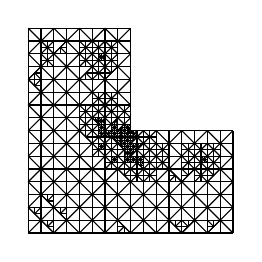
\begin{tikzpicture}[scale = 1.3]
\draw (0.250000,0.000000)  -- (0.250000,-0.125000);
\draw (0.000000,0.250000)  -- (-0.125000,0.250000);
\draw (0.000000,-0.500000)  -- (-0.125000,-0.375000);
\draw (-0.500000,0.000000)  -- (-0.375000,-0.125000);
\draw (-0.125000,0.125000)  -- (-0.062500,0.062500);
\draw (0.125000,-0.125000)  -- (0.062500,-0.062500);
\draw (-0.125000,0.000000)  -- (-0.062500,0.062500);
\draw (0.000000,-0.125000)  -- (0.062500,-0.062500);
\draw (-0.125000,0.125000)  -- (-0.125000,0.062500);
\draw (0.125000,-0.125000)  -- (0.062500,-0.125000);
\draw (-0.125000,0.000000)  -- (-0.125000,0.062500);
\draw (0.000000,-0.125000)  -- (0.062500,-0.125000);
\draw (0.062500,-0.062500)  -- (0.062500,-0.125000);
\draw (-0.062500,0.062500)  -- (-0.125000,0.062500);
\draw (0.000000,0.125000)  -- (-0.062500,0.062500);
\draw (0.125000,0.000000)  -- (0.062500,-0.062500);
\draw (0.125000,-0.125000)  -- (0.125000,-0.062500);
\draw (-0.125000,0.125000)  -- (-0.062500,0.125000);
\draw (0.000000,0.125000)  -- (0.000000,0.062500);
\draw (0.125000,0.000000)  -- (0.062500,0.000000);
\draw (0.125000,0.000000)  -- (0.125000,-0.062500);
\draw (0.000000,0.125000)  -- (-0.062500,0.125000);
\draw (-0.062500,0.062500)  -- (-0.062500,0.125000);
\draw (0.062500,-0.062500)  -- (0.062500,0.000000);
\draw (-0.062500,0.062500)  -- (0.000000,0.062500);
\draw (0.062500,-0.062500)  -- (0.125000,-0.062500);
\draw (0.500000,0.000000)  -- (0.625000,-0.125000);
\draw (0.000000,0.500000)  -- (-0.125000,0.625000);
\draw (-0.250000,0.500000)  -- (-0.125000,0.625000);
\draw (0.500000,0.000000)  -- (0.500000,-0.125000);
\draw (0.000000,0.500000)  -- (-0.125000,0.500000);
\draw (0.500000,-0.250000)  -- (0.500000,-0.125000);
\draw (-0.250000,0.500000)  -- (-0.125000,0.500000);
\draw (-0.125000,0.625000)  -- (-0.125000,0.500000);
\draw (0.625000,-0.125000)  -- (0.500000,-0.125000);
\draw (1.000000,-1.000000)  -- (0.875000,-0.875000);
\draw (-1.000000,1.000000)  -- (-0.875000,0.875000);
\draw (0.500000,-0.500000)  -- (0.625000,-0.375000);
\draw (-0.500000,0.500000)  -- (-0.375000,0.625000);
\draw (-0.500000,1.000000)  -- (-0.375000,0.875000);
\draw (1.000000,-0.500000)  -- (0.875000,-0.375000);
\draw (0.750000,-0.750000)  -- (0.875000,-0.875000);
\draw (-0.062500,-0.062500)  -- (-0.031250,-0.031250);
\draw (-0.062500,0.000000)  -- (-0.031250,-0.031250);
\draw (0.000000,-0.062500)  -- (-0.031250,-0.031250);
\draw (-0.250000,-0.500000)  -- (-0.125000,-0.375000);
\draw (-0.500000,-0.250000)  -- (-0.375000,-0.125000);
\draw (0.750000,-0.500000)  -- (0.875000,-0.375000);
\draw (0.750000,-1.000000)  -- (0.875000,-0.875000);
\draw (-1.000000,0.750000)  -- (-0.875000,0.875000);
\draw (1.000000,-0.750000)  -- (0.875000,-0.875000);
\draw (0.000000,-0.500000)  -- (-0.125000,-0.500000);
\draw (-0.500000,0.000000)  -- (-0.500000,-0.125000);
\draw (-0.250000,-0.250000)  -- (-0.375000,-0.250000);
\draw (-0.250000,-0.250000)  -- (-0.250000,-0.375000);
\draw (0.500000,-0.500000)  -- (0.500000,-0.375000);
\draw (-0.500000,0.500000)  -- (-0.375000,0.500000);
\draw (1.000000,-1.000000)  -- (1.000000,-0.875000);
\draw (-1.000000,1.000000)  -- (-1.000000,0.875000);
\draw (1.000000,-1.000000)  -- (0.875000,-1.000000);
\draw (-0.500000,1.000000)  -- (-0.500000,0.875000);
\draw (1.000000,-0.500000)  -- (0.875000,-0.500000);
\draw (0.750000,-0.750000)  -- (0.750000,-0.875000);
\draw (0.750000,-0.750000)  -- (0.875000,-0.750000);
\draw (-0.062500,-0.062500)  -- (-0.031250,-0.062500);
\draw (-0.062500,-0.062500)  -- (-0.062500,-0.031250);
\draw (-0.250000,-0.500000)  -- (-0.125000,-0.500000);
\draw (-0.500000,-0.250000)  -- (-0.500000,-0.125000);
\draw (-0.500000,-0.250000)  -- (-0.375000,-0.250000);
\draw (-0.250000,-0.500000)  -- (-0.250000,-0.375000);
\draw (0.500000,-0.250000)  -- (0.500000,-0.375000);
\draw (-0.250000,0.500000)  -- (-0.375000,0.500000);
\draw (1.000000,-0.750000)  -- (1.000000,-0.875000);
\draw (-1.000000,0.750000)  -- (-1.000000,0.875000);
\draw (0.750000,-1.000000)  -- (0.875000,-1.000000);
\draw (-0.500000,0.750000)  -- (-0.500000,0.875000);
\draw (0.750000,-0.500000)  -- (0.875000,-0.500000);
\draw (0.750000,-1.000000)  -- (0.750000,-0.875000);
\draw (-1.000000,0.750000)  -- (-0.875000,0.750000);
\draw (1.000000,-0.750000)  -- (0.875000,-0.750000);
\draw (0.000000,-0.062500)  -- (0.000000,-0.031250);
\draw (-0.062500,0.000000)  -- (-0.031250,0.000000);
\draw (0.000000,-0.062500)  -- (-0.031250,-0.062500);
\draw (-0.062500,0.000000)  -- (-0.062500,-0.031250);
\draw (-0.031250,-0.031250)  -- (-0.062500,-0.031250);
\draw (-0.031250,-0.031250)  -- (0.000000,-0.031250);
\draw (-0.125000,-0.375000)  -- (-0.125000,-0.500000);
\draw (-0.375000,-0.125000)  -- (-0.375000,-0.250000);
\draw (0.875000,-0.375000)  -- (0.875000,-0.500000);
\draw (0.875000,-0.875000)  -- (0.875000,-1.000000);
\draw (-0.875000,0.875000)  -- (-0.875000,0.750000);
\draw (0.875000,-0.875000)  -- (0.875000,-0.750000);
\draw (-0.031250,-0.031250)  -- (-0.031250,0.000000);
\draw (-0.031250,-0.031250)  -- (-0.031250,-0.062500);
\draw (-0.125000,-0.375000)  -- (-0.250000,-0.375000);
\draw (-0.375000,-0.125000)  -- (-0.500000,-0.125000);
\draw (0.875000,-0.875000)  -- (0.750000,-0.875000);
\draw (-0.375000,0.875000)  -- (-0.500000,0.875000);
\draw (-0.875000,0.875000)  -- (-1.000000,0.875000);
\draw (0.875000,-0.875000)  -- (1.000000,-0.875000);
\draw (-0.500000,-0.500000)  -- (-0.375000,-0.375000);
\draw (-1.000000,-1.000000)  -- (-0.875000,-0.875000);
\draw (0.500000,-1.000000)  -- (0.625000,-0.875000);
\draw (-1.000000,0.500000)  -- (-0.875000,0.625000);
\draw (-0.500000,1.000000)  -- (-0.625000,0.875000);
\draw (1.000000,-0.500000)  -- (0.875000,-0.625000);
\draw (-0.250000,-0.250000)  -- (-0.312500,-0.187500);
\draw (-1.000000,0.500000)  -- (-0.875000,0.375000);
\draw (0.500000,-1.000000)  -- (0.375000,-0.875000);
\draw (-0.250000,-0.250000)  -- (-0.375000,-0.375000);
\draw (-0.750000,-0.750000)  -- (-0.875000,-0.875000);
\draw (-0.125000,-0.125000)  -- (-0.187500,-0.062500);
\draw (-0.125000,-0.125000)  -- (-0.062500,-0.187500);
\draw (0.750000,-0.750000)  -- (0.625000,-0.875000);
\draw (-0.750000,0.750000)  -- (-0.625000,0.875000);
\draw (0.750000,-0.750000)  -- (0.875000,-0.625000);
\draw (-0.375000,-0.125000)  -- (-0.312500,-0.187500);
\draw (-0.750000,0.250000)  -- (-0.875000,0.375000);
\draw (-0.375000,-0.125000)  -- (-0.312500,-0.062500);
\draw (-0.125000,-0.375000)  -- (-0.062500,-0.312500);
\draw (0.250000,-0.750000)  -- (0.375000,-0.875000);
\draw (-0.375000,0.125000)  -- (-0.312500,0.062500);
\draw (0.125000,-0.375000)  -- (0.062500,-0.312500);
\draw (-0.750000,-1.000000)  -- (-0.875000,-0.875000);
\draw (-1.000000,-0.750000)  -- (-0.875000,-0.875000);
\draw (-0.750000,1.000000)  -- (-0.875000,0.875000);
\draw (-0.250000,-0.125000)  -- (-0.312500,-0.062500);
\draw (-0.375000,0.000000)  -- (-0.312500,-0.062500);
\draw (-0.125000,-0.250000)  -- (-0.062500,-0.312500);
\draw (-0.500000,0.750000)  -- (-0.625000,0.875000);
\draw (-1.000000,0.250000)  -- (-0.875000,0.375000);
\draw (0.000000,-0.375000)  -- (-0.062500,-0.312500);
\draw (-0.250000,-0.500000)  -- (-0.375000,-0.375000);
\draw (-0.500000,-0.250000)  -- (-0.375000,-0.375000);
\draw (0.500000,-0.750000)  -- (0.625000,-0.875000);
\draw (-0.250000,-0.125000)  -- (-0.187500,-0.062500);
\draw (-0.375000,0.000000)  -- (-0.312500,0.062500);
\draw (0.250000,-1.000000)  -- (0.375000,-0.875000);
\draw (-0.125000,-0.250000)  -- (-0.062500,-0.187500);
\draw (0.750000,-0.500000)  -- (0.875000,-0.625000);
\draw (0.000000,-0.375000)  -- (0.062500,-0.312500);
\draw (-0.750000,0.500000)  -- (-0.875000,0.625000);
\draw (-0.500000,-0.500000)  -- (-0.375000,-0.500000);
\draw (-0.500000,-0.500000)  -- (-0.500000,-0.375000);
\draw (-1.000000,-1.000000)  -- (-0.875000,-1.000000);
\draw (-1.000000,-1.000000)  -- (-1.000000,-0.875000);
\draw (-1.000000,1.000000)  -- (-0.875000,1.000000);
\draw (-0.500000,0.500000)  -- (-0.500000,0.625000);
\draw (0.500000,-0.500000)  -- (0.625000,-0.500000);
\draw (-0.250000,-0.250000)  -- (-0.250000,-0.187500);
\draw (-0.250000,0.000000)  -- (-0.187500,0.000000);
\draw (-0.125000,-0.125000)  -- (-0.187500,-0.125000);
\draw (-0.750000,0.750000)  -- (-0.750000,0.625000);
\draw (-0.750000,-0.750000)  -- (-0.875000,-0.750000);
\draw (-0.750000,0.750000)  -- (-0.750000,0.875000);
\draw (0.750000,-0.750000)  -- (0.750000,-0.625000);
\draw (-0.125000,-0.125000)  -- (-0.125000,-0.187500);
\draw (0.750000,-0.750000)  -- (0.625000,-0.750000);
\draw (-0.750000,-0.750000)  -- (-0.750000,-0.875000);
\draw (-0.750000,0.750000)  -- (-0.625000,0.750000);
\draw (-0.250000,0.000000)  -- (-0.250000,0.062500);
\draw (0.000000,-0.250000)  -- (0.062500,-0.250000);
\draw (0.500000,-1.000000)  -- (0.375000,-1.000000);
\draw (-1.000000,0.500000)  -- (-1.000000,0.375000);
\draw (-0.750000,0.250000)  -- (-0.875000,0.250000);
\draw (-0.375000,-0.125000)  -- (-0.375000,-0.062500);
\draw (-0.125000,-0.375000)  -- (-0.125000,-0.312500);
\draw (-0.375000,0.125000)  -- (-0.312500,0.125000);
\draw (0.125000,-0.375000)  -- (0.062500,-0.375000);
\draw (-0.375000,-0.125000)  -- (-0.312500,-0.125000);
\draw (-0.125000,-0.375000)  -- (-0.062500,-0.375000);
\draw (0.250000,-0.750000)  -- (0.250000,-0.875000);
\draw (-0.375000,0.125000)  -- (-0.375000,0.062500);
\draw (0.125000,-0.375000)  -- (0.125000,-0.312500);
\draw (-0.250000,-0.500000)  -- (-0.375000,-0.500000);
\draw (-0.500000,-0.250000)  -- (-0.500000,-0.375000);
\draw (-0.750000,-1.000000)  -- (-0.875000,-1.000000);
\draw (-1.000000,-0.750000)  -- (-1.000000,-0.875000);
\draw (-0.750000,1.000000)  -- (-0.875000,1.000000);
\draw (-0.500000,0.750000)  -- (-0.500000,0.625000);
\draw (0.750000,-0.500000)  -- (0.625000,-0.500000);
\draw (-0.250000,-0.125000)  -- (-0.250000,-0.187500);
\draw (0.500000,-0.750000)  -- (0.500000,-0.875000);
\draw (-0.750000,0.500000)  -- (-0.875000,0.500000);
\draw (-0.125000,-0.250000)  -- (-0.062500,-0.250000);
\draw (-0.250000,-0.125000)  -- (-0.250000,-0.062500);
\draw (-0.250000,-0.125000)  -- (-0.187500,-0.125000);
\draw (-0.750000,0.500000)  -- (-0.750000,0.625000);
\draw (-1.000000,-0.750000)  -- (-0.875000,-0.750000);
\draw (-0.750000,1.000000)  -- (-0.750000,0.875000);
\draw (0.750000,-0.500000)  -- (0.750000,-0.625000);
\draw (-0.125000,-0.250000)  -- (-0.125000,-0.187500);
\draw (0.500000,-0.750000)  -- (0.625000,-0.750000);
\draw (-0.750000,-1.000000)  -- (-0.750000,-0.875000);
\draw (-0.500000,0.750000)  -- (-0.625000,0.750000);
\draw (-0.250000,0.125000)  -- (-0.250000,0.062500);
\draw (0.125000,-0.250000)  -- (0.062500,-0.250000);
\draw (0.250000,-1.000000)  -- (0.375000,-1.000000);
\draw (-1.000000,0.250000)  -- (-1.000000,0.375000);
\draw (0.000000,-0.375000)  -- (0.000000,-0.312500);
\draw (-0.375000,0.000000)  -- (-0.312500,0.000000);
\draw (-1.000000,0.250000)  -- (-0.875000,0.250000);
\draw (-0.375000,0.000000)  -- (-0.375000,-0.062500);
\draw (-0.125000,-0.250000)  -- (-0.125000,-0.312500);
\draw (-0.250000,0.125000)  -- (-0.312500,0.125000);
\draw (0.000000,-0.375000)  -- (0.062500,-0.375000);
\draw (-0.250000,-0.125000)  -- (-0.312500,-0.125000);
\draw (0.000000,-0.375000)  -- (-0.062500,-0.375000);
\draw (0.250000,-1.000000)  -- (0.250000,-0.875000);
\draw (-0.375000,0.000000)  -- (-0.375000,0.062500);
\draw (0.125000,-0.250000)  -- (0.125000,-0.312500);
\draw (-0.875000,-0.875000)  -- (-0.750000,-0.875000);
\draw (-0.875000,-0.875000)  -- (-1.000000,-0.875000);
\draw (-0.375000,0.625000)  -- (-0.500000,0.625000);
\draw (-0.875000,0.875000)  -- (-0.875000,1.000000);
\draw (-0.312500,-0.062500)  -- (-0.250000,-0.062500);
\draw (-0.312500,-0.062500)  -- (-0.375000,-0.062500);
\draw (-0.062500,-0.312500)  -- (-0.125000,-0.312500);
\draw (-0.625000,0.875000)  -- (-0.500000,0.875000);
\draw (-0.875000,0.375000)  -- (-0.875000,0.250000);
\draw (-0.062500,-0.312500)  -- (0.000000,-0.312500);
\draw (-0.375000,-0.375000)  -- (-0.250000,-0.375000);
\draw (-0.375000,-0.375000)  -- (-0.500000,-0.375000);
\draw (0.625000,-0.875000)  -- (0.500000,-0.875000);
\draw (-0.187500,-0.062500)  -- (-0.187500,-0.125000);
\draw (-0.312500,0.062500)  -- (-0.312500,0.000000);
\draw (0.375000,-0.875000)  -- (0.375000,-1.000000);
\draw (-0.062500,-0.187500)  -- (-0.062500,-0.250000);
\draw (0.875000,-0.625000)  -- (0.750000,-0.625000);
\draw (0.062500,-0.312500)  -- (0.062500,-0.375000);
\draw (-0.875000,0.625000)  -- (-0.750000,0.625000);
\draw (-0.312500,-0.187500)  -- (-0.312500,-0.125000);
\draw (-0.875000,-0.875000)  -- (-0.875000,-1.000000);
\draw (-0.875000,-0.875000)  -- (-0.875000,-0.750000);
\draw (0.625000,-0.375000)  -- (0.625000,-0.500000);
\draw (-0.875000,0.875000)  -- (-0.750000,0.875000);
\draw (-0.312500,-0.062500)  -- (-0.312500,-0.125000);
\draw (-0.312500,-0.062500)  -- (-0.312500,0.000000);
\draw (-0.062500,-0.312500)  -- (-0.062500,-0.250000);
\draw (-0.625000,0.875000)  -- (-0.625000,0.750000);
\draw (-0.875000,0.375000)  -- (-1.000000,0.375000);
\draw (-0.062500,-0.312500)  -- (-0.062500,-0.375000);
\draw (-0.375000,-0.375000)  -- (-0.375000,-0.500000);
\draw (-0.375000,-0.375000)  -- (-0.375000,-0.250000);
\draw (0.625000,-0.875000)  -- (0.625000,-0.750000);
\draw (-0.187500,-0.062500)  -- (-0.250000,-0.062500);
\draw (-0.312500,0.062500)  -- (-0.375000,0.062500);
\draw (0.375000,-0.875000)  -- (0.250000,-0.875000);
\draw (-0.062500,-0.187500)  -- (-0.125000,-0.187500);
\draw (0.875000,-0.625000)  -- (0.875000,-0.500000);
\draw (0.062500,-0.312500)  -- (0.000000,-0.312500);
\draw (-0.875000,0.625000)  -- (-0.875000,0.500000);
\draw (-0.312500,-0.187500)  -- (-0.250000,-0.187500);
\draw (1.000000,0.000000)  -- (0.875000,-0.125000);
\draw (0.000000,1.000000)  -- (-0.125000,0.875000);
\draw (0.000000,0.750000)  -- (-0.125000,0.625000);
\draw (0.750000,0.000000)  -- (0.875000,-0.125000);
\draw (0.000000,0.750000)  -- (-0.125000,0.875000);
\draw (-1.000000,0.750000)  -- (-0.875000,0.625000);
\draw (0.750000,0.000000)  -- (0.625000,-0.125000);
\draw (1.000000,-0.250000)  -- (0.875000,-0.375000);
\draw (-0.250000,1.000000)  -- (-0.125000,0.875000);
\draw (1.000000,-0.250000)  -- (0.875000,-0.125000);
\draw (-0.250000,1.000000)  -- (-0.375000,0.875000);
\draw (1.000000,0.000000)  -- (0.875000,0.000000);
\draw (0.000000,1.000000)  -- (0.000000,0.875000);
\draw (-1.000000,0.500000)  -- (-1.000000,0.625000);
\draw (0.500000,0.000000)  -- (0.625000,0.000000);
\draw (0.000000,0.500000)  -- (0.000000,0.625000);
\draw (0.000000,1.000000)  -- (-0.125000,1.000000);
\draw (1.000000,0.000000)  -- (1.000000,-0.125000);
\draw (-0.500000,1.000000)  -- (-0.375000,1.000000);
\draw (1.000000,-0.500000)  -- (1.000000,-0.375000);
\draw (0.750000,0.000000)  -- (0.875000,0.000000);
\draw (0.000000,0.750000)  -- (0.000000,0.875000);
\draw (-1.000000,0.750000)  -- (-1.000000,0.625000);
\draw (0.750000,0.000000)  -- (0.625000,0.000000);
\draw (0.000000,0.750000)  -- (0.000000,0.625000);
\draw (0.000000,0.750000)  -- (-0.125000,0.750000);
\draw (0.750000,0.000000)  -- (0.750000,-0.125000);
\draw (-0.250000,1.000000)  -- (-0.125000,1.000000);
\draw (1.000000,-0.250000)  -- (1.000000,-0.125000);
\draw (-0.250000,1.000000)  -- (-0.375000,1.000000);
\draw (1.000000,-0.250000)  -- (1.000000,-0.375000);
\draw (1.000000,-0.250000)  -- (0.875000,-0.250000);
\draw (-0.250000,1.000000)  -- (-0.250000,0.875000);
\draw (-0.125000,0.625000)  -- (-0.125000,0.750000);
\draw (0.875000,-0.125000)  -- (0.750000,-0.125000);
\draw (-0.125000,0.875000)  -- (0.000000,0.875000);
\draw (-0.875000,0.625000)  -- (-1.000000,0.625000);
\draw (0.625000,-0.125000)  -- (0.625000,0.000000);
\draw (0.875000,-0.375000)  -- (0.875000,-0.250000);
\draw (-0.125000,0.875000)  -- (-0.250000,0.875000);
\draw (0.875000,-0.125000)  -- (1.000000,-0.125000);
\draw (-0.375000,0.875000)  -- (-0.375000,1.000000);
\draw (-0.125000,0.625000)  -- (0.000000,0.625000);
\draw (0.875000,-0.125000)  -- (0.875000,0.000000);
\draw (-0.125000,0.875000)  -- (-0.125000,0.750000);
\draw (-0.875000,0.625000)  -- (-0.875000,0.750000);
\draw (0.625000,-0.125000)  -- (0.750000,-0.125000);
\draw (0.875000,-0.375000)  -- (1.000000,-0.375000);
\draw (-0.125000,0.875000)  -- (-0.125000,1.000000);
\draw (0.875000,-0.125000)  -- (0.875000,-0.250000);
\draw (-0.375000,0.875000)  -- (-0.250000,0.875000);
\draw (0.500000,-0.500000)  -- (0.375000,-0.375000);
\draw (-0.250000,-0.250000)  -- (-0.187500,-0.187500);
\draw (0.000000,-0.250000)  -- (0.062500,-0.187500);
\draw (-0.250000,0.000000)  -- (-0.187500,0.062500);
\draw (-1.000000,0.000000)  -- (-0.875000,0.125000);
\draw (-0.250000,-0.250000)  -- (-0.187500,-0.312500);
\draw (-1.000000,-0.500000)  -- (-0.875000,-0.375000);
\draw (-0.500000,-1.000000)  -- (-0.375000,-0.875000);
\draw (-0.125000,-0.125000)  -- (-0.187500,-0.187500);
\draw (0.125000,-0.125000)  -- (0.062500,-0.187500);
\draw (-0.125000,0.125000)  -- (-0.187500,0.062500);
\draw (-0.750000,0.250000)  -- (-0.875000,0.125000);
\draw (-0.125000,-0.375000)  -- (-0.187500,-0.312500);
\draw (-0.750000,-0.250000)  -- (-0.875000,-0.375000);
\draw (-0.250000,-0.750000)  -- (-0.375000,-0.875000);
\draw (-0.125000,-0.250000)  -- (-0.187500,-0.187500);
\draw (0.500000,-0.250000)  -- (0.375000,-0.375000);
\draw (-0.250000,-0.125000)  -- (-0.187500,-0.187500);
\draw (-0.750000,1.000000)  -- (-0.625000,0.875000);
\draw (-1.000000,0.250000)  -- (-0.875000,0.125000);
\draw (-0.250000,-1.000000)  -- (-0.375000,-0.875000);
\draw (-0.750000,0.500000)  -- (-0.875000,0.375000);
\draw (-1.000000,-0.250000)  -- (-0.875000,-0.375000);
\draw (-0.250000,-0.250000)  -- (-0.187500,-0.250000);
\draw (-0.500000,1.000000)  -- (-0.625000,1.000000);
\draw (-1.000000,0.000000)  -- (-1.000000,0.125000);
\draw (-1.000000,-0.500000)  -- (-1.000000,-0.375000);
\draw (-0.500000,-1.000000)  -- (-0.375000,-1.000000);
\draw (-0.250000,-0.750000)  -- (-0.250000,-0.875000);
\draw (-0.750000,0.250000)  -- (-0.750000,0.375000);
\draw (-0.750000,-0.250000)  -- (-0.875000,-0.250000);
\draw (0.500000,-0.250000)  -- (0.375000,-0.250000);
\draw (-0.125000,-0.250000)  -- (-0.187500,-0.250000);
\draw (-0.750000,1.000000)  -- (-0.625000,1.000000);
\draw (-1.000000,0.250000)  -- (-1.000000,0.125000);
\draw (-1.000000,-0.250000)  -- (-1.000000,-0.375000);
\draw (-0.250000,-1.000000)  -- (-0.375000,-1.000000);
\draw (-0.250000,-1.000000)  -- (-0.250000,-0.875000);
\draw (-0.750000,0.500000)  -- (-0.750000,0.375000);
\draw (-1.000000,-0.250000)  -- (-0.875000,-0.250000);
\draw (-0.187500,-0.187500)  -- (-0.125000,-0.187500);
\draw (0.375000,-0.375000)  -- (0.375000,-0.250000);
\draw (-0.187500,-0.187500)  -- (-0.250000,-0.187500);
\draw (-0.625000,0.875000)  -- (-0.750000,0.875000);
\draw (-0.875000,0.125000)  -- (-1.000000,0.125000);
\draw (-0.375000,-0.875000)  -- (-0.250000,-0.875000);
\draw (-0.187500,-0.312500)  -- (-0.187500,-0.250000);
\draw (-0.875000,0.375000)  -- (-0.875000,0.500000);
\draw (-0.875000,-0.375000)  -- (-1.000000,-0.375000);
\draw (-0.187500,-0.187500)  -- (-0.187500,-0.250000);
\draw (0.375000,-0.375000)  -- (0.500000,-0.375000);
\draw (-0.187500,-0.187500)  -- (-0.187500,-0.125000);
\draw (-0.625000,0.875000)  -- (-0.625000,1.000000);
\draw (-0.875000,0.125000)  -- (-0.875000,0.250000);
\draw (-0.375000,-0.875000)  -- (-0.375000,-1.000000);
\draw (-0.187500,-0.312500)  -- (-0.125000,-0.312500);
\draw (-0.875000,0.375000)  -- (-0.750000,0.375000);
\draw (-0.875000,-0.375000)  -- (-0.875000,-0.250000);
\draw (-0.187500,0.062500)  -- (-0.187500,0.000000);
\draw (-0.500000,0.500000)  -- (-0.375000,0.375000);
\draw (0.000000,0.500000)  -- (-0.125000,0.375000);
\draw (0.500000,0.000000)  -- (0.375000,-0.125000);
\draw (-0.062500,0.062500)  -- (-0.031250,0.031250);
\draw (0.062500,-0.062500)  -- (0.031250,-0.031250);
\draw (-0.500000,0.250000)  -- (-0.375000,0.375000);
\draw (0.250000,-0.500000)  -- (0.375000,-0.375000);
\draw (-0.250000,0.500000)  -- (-0.125000,0.375000);
\draw (0.250000,0.000000)  -- (0.375000,-0.125000);
\draw (-0.250000,0.500000)  -- (-0.375000,0.375000);
\draw (0.000000,0.250000)  -- (-0.125000,0.375000);
\draw (0.500000,-0.250000)  -- (0.375000,-0.125000);
\draw (0.000000,-0.062500)  -- (0.031250,-0.031250);
\draw (-0.062500,0.000000)  -- (-0.031250,0.031250);
\draw (0.000000,0.062500)  -- (-0.031250,0.031250);
\draw (0.062500,0.000000)  -- (0.031250,-0.031250);
\draw (-0.500000,0.500000)  -- (-0.500000,0.375000);
\draw (0.500000,-0.500000)  -- (0.375000,-0.500000);
\draw (-0.500000,0.000000)  -- (-0.500000,0.125000);
\draw (0.000000,-0.500000)  -- (0.125000,-0.500000);
\draw (0.000000,0.500000)  -- (0.000000,0.375000);
\draw (0.500000,0.000000)  -- (0.375000,0.000000);
\draw (-0.062500,0.062500)  -- (-0.062500,0.031250);
\draw (0.062500,-0.062500)  -- (0.031250,-0.062500);
\draw (0.062500,-0.062500)  -- (0.062500,-0.031250);
\draw (-0.062500,0.062500)  -- (-0.031250,0.062500);
\draw (-0.500000,0.250000)  -- (-0.500000,0.375000);
\draw (0.250000,-0.500000)  -- (0.375000,-0.500000);
\draw (-0.500000,0.250000)  -- (-0.500000,0.125000);
\draw (0.250000,-0.500000)  -- (0.125000,-0.500000);
\draw (0.250000,-0.500000)  -- (0.250000,-0.375000);
\draw (-0.500000,0.250000)  -- (-0.375000,0.250000);
\draw (0.000000,0.250000)  -- (0.000000,0.375000);
\draw (0.250000,0.000000)  -- (0.375000,0.000000);
\draw (-0.250000,0.500000)  -- (-0.250000,0.375000);
\draw (-0.062500,0.000000)  -- (-0.062500,0.031250);
\draw (0.000000,-0.062500)  -- (0.031250,-0.062500);
\draw (0.000000,0.062500)  -- (0.000000,0.031250);
\draw (0.062500,0.000000)  -- (0.031250,0.000000);
\draw (0.062500,0.000000)  -- (0.062500,-0.031250);
\draw (0.000000,0.062500)  -- (-0.031250,0.062500);
\draw (-0.375000,0.375000)  -- (-0.375000,0.250000);
\draw (0.375000,-0.375000)  -- (0.375000,-0.500000);
\draw (-0.125000,0.375000)  -- (-0.250000,0.375000);
\draw (0.375000,-0.125000)  -- (0.250000,-0.125000);
\draw (-0.375000,0.375000)  -- (-0.375000,0.500000);
\draw (-0.125000,0.375000)  -- (0.000000,0.375000);
\draw (0.375000,-0.125000)  -- (0.500000,-0.125000);
\draw (0.031250,-0.031250)  -- (0.031250,-0.062500);
\draw (-0.031250,0.031250)  -- (-0.031250,0.000000);
\draw (-0.031250,0.031250)  -- (-0.031250,0.062500);
\draw (0.031250,-0.031250)  -- (0.031250,0.000000);
\draw (-0.375000,0.375000)  -- (-0.500000,0.375000);
\draw (0.375000,-0.375000)  -- (0.250000,-0.375000);
\draw (-0.125000,0.375000)  -- (-0.125000,0.500000);
\draw (0.375000,-0.125000)  -- (0.375000,0.000000);
\draw (-0.375000,0.375000)  -- (-0.250000,0.375000);
\draw (-0.125000,0.375000)  -- (-0.125000,0.250000);
\draw (0.375000,-0.125000)  -- (0.375000,-0.250000);
\draw (0.031250,-0.031250)  -- (0.000000,-0.031250);
\draw (-0.031250,0.031250)  -- (-0.062500,0.031250);
\draw (-0.031250,0.031250)  -- (0.000000,0.031250);
\draw (0.031250,-0.031250)  -- (0.062500,-0.031250);
\draw (-1.000000,-0.500000)  -- (-0.875000,-0.625000);
\draw (-0.500000,-1.000000)  -- (-0.625000,-0.875000);
\draw (0.000000,-1.000000)  -- (0.125000,-0.875000);
\draw (-1.000000,0.000000)  -- (-0.875000,-0.125000);
\draw (0.250000,-0.250000)  -- (0.187500,-0.312500);
\draw (-0.250000,0.250000)  -- (-0.312500,0.187500);
\draw (-0.750000,-0.750000)  -- (-0.875000,-0.625000);
\draw (-0.750000,-0.750000)  -- (-0.625000,-0.875000);
\draw (0.250000,-0.750000)  -- (0.125000,-0.875000);
\draw (-0.750000,-0.250000)  -- (-0.875000,-0.125000);
\draw (0.125000,-0.375000)  -- (0.187500,-0.312500);
\draw (-0.375000,0.125000)  -- (-0.312500,0.187500);
\draw (0.625000,-0.375000)  -- (0.687500,-0.312500);
\draw (-0.375000,0.625000)  -- (-0.312500,0.687500);
\draw (0.500000,-0.750000)  -- (0.375000,-0.875000);
\draw (-0.750000,-0.500000)  -- (-0.875000,-0.625000);
\draw (-1.000000,-0.250000)  -- (-0.875000,-0.125000);
\draw (0.750000,-1.000000)  -- (0.625000,-0.875000);
\draw (0.750000,-0.375000)  -- (0.687500,-0.312500);
\draw (0.625000,-0.250000)  -- (0.687500,-0.312500);
\draw (0.250000,-1.000000)  -- (0.125000,-0.875000);
\draw (-0.500000,-0.750000)  -- (-0.625000,-0.875000);
\draw (-0.250000,0.625000)  -- (-0.312500,0.687500);
\draw (-0.375000,0.750000)  -- (-0.312500,0.687500);
\draw (0.125000,-0.250000)  -- (0.187500,-0.312500);
\draw (-0.250000,0.125000)  -- (-0.312500,0.187500);
\draw (-0.750000,-0.500000)  -- (-0.875000,-0.375000);
\draw (0.500000,-1.000000)  -- (0.625000,-1.000000);
\draw (-1.000000,-0.500000)  -- (-0.875000,-0.500000);
\draw (-0.500000,-1.000000)  -- (-0.500000,-0.875000);
\draw (-0.750000,-0.750000)  -- (-0.625000,-0.750000);
\draw (-0.750000,-0.750000)  -- (-0.750000,-0.625000);
\draw (-0.250000,0.250000)  -- (-0.250000,0.187500);
\draw (0.250000,-0.250000)  -- (0.187500,-0.250000);
\draw (0.000000,-1.000000)  -- (0.125000,-1.000000);
\draw (-1.000000,0.000000)  -- (-1.000000,-0.125000);
\draw (0.250000,-0.750000)  -- (0.375000,-0.750000);
\draw (-0.750000,-0.250000)  -- (-0.750000,-0.375000);
\draw (0.750000,-0.250000)  -- (0.687500,-0.250000);
\draw (-0.250000,0.750000)  -- (-0.250000,0.687500);
\draw (-0.250000,0.750000)  -- (-0.312500,0.750000);
\draw (0.750000,-0.250000)  -- (0.750000,-0.312500);
\draw (-0.375000,0.625000)  -- (-0.312500,0.625000);
\draw (0.625000,-0.375000)  -- (0.625000,-0.312500);
\draw (0.625000,-0.375000)  -- (0.687500,-0.375000);
\draw (-0.375000,0.625000)  -- (-0.375000,0.687500);
\draw (0.750000,-1.000000)  -- (0.625000,-1.000000);
\draw (-0.750000,-0.500000)  -- (-0.875000,-0.500000);
\draw (-0.500000,-0.750000)  -- (-0.500000,-0.875000);
\draw (-0.500000,-0.750000)  -- (-0.625000,-0.750000);
\draw (-0.750000,-0.500000)  -- (-0.750000,-0.625000);
\draw (-0.250000,0.125000)  -- (-0.250000,0.187500);
\draw (0.125000,-0.250000)  -- (0.187500,-0.250000);
\draw (0.250000,-1.000000)  -- (0.125000,-1.000000);
\draw (-1.000000,-0.250000)  -- (-1.000000,-0.125000);
\draw (0.500000,-0.750000)  -- (0.375000,-0.750000);
\draw (-0.750000,-0.500000)  -- (-0.750000,-0.375000);
\draw (0.625000,-0.250000)  -- (0.687500,-0.250000);
\draw (-0.250000,0.625000)  -- (-0.250000,0.687500);
\draw (-0.375000,0.750000)  -- (-0.312500,0.750000);
\draw (0.750000,-0.375000)  -- (0.750000,-0.312500);
\draw (-0.250000,0.625000)  -- (-0.312500,0.625000);
\draw (0.625000,-0.250000)  -- (0.625000,-0.312500);
\draw (0.750000,-0.375000)  -- (0.687500,-0.375000);
\draw (-0.375000,0.750000)  -- (-0.375000,0.687500);
\draw (0.375000,-0.875000)  -- (0.375000,-0.750000);
\draw (-0.875000,-0.625000)  -- (-0.875000,-0.500000);
\draw (-0.875000,-0.125000)  -- (-0.875000,-0.250000);
\draw (0.625000,-0.875000)  -- (0.750000,-0.875000);
\draw (0.687500,-0.312500)  -- (0.750000,-0.312500);
\draw (0.687500,-0.312500)  -- (0.625000,-0.312500);
\draw (0.125000,-0.875000)  -- (0.250000,-0.875000);
\draw (-0.625000,-0.875000)  -- (-0.625000,-0.750000);
\draw (-0.312500,0.687500)  -- (-0.250000,0.687500);
\draw (-0.312500,0.687500)  -- (-0.375000,0.687500);
\draw (0.187500,-0.312500)  -- (0.125000,-0.312500);
\draw (-0.312500,0.187500)  -- (-0.250000,0.187500);
\draw (-0.875000,-0.375000)  -- (-0.750000,-0.375000);
\draw (0.375000,-0.875000)  -- (0.500000,-0.875000);
\draw (-0.875000,-0.625000)  -- (-0.750000,-0.625000);
\draw (-0.875000,-0.125000)  -- (-1.000000,-0.125000);
\draw (0.625000,-0.875000)  -- (0.625000,-1.000000);
\draw (0.687500,-0.312500)  -- (0.687500,-0.375000);
\draw (0.687500,-0.312500)  -- (0.687500,-0.250000);
\draw (0.125000,-0.875000)  -- (0.125000,-1.000000);
\draw (-0.625000,-0.875000)  -- (-0.500000,-0.875000);
\draw (-0.312500,0.687500)  -- (-0.312500,0.625000);
\draw (-0.312500,0.687500)  -- (-0.312500,0.750000);
\draw (0.187500,-0.312500)  -- (0.187500,-0.250000);
\draw (-0.312500,0.187500)  -- (-0.312500,0.125000);
\draw (-0.875000,-0.375000)  -- (-0.875000,-0.500000);
\draw (0.000000,0.000000)  -- (-0.015625,-0.015625);
\draw (-0.031250,-0.031250)  -- (-0.015625,-0.015625);
\draw (1.000000,-0.750000)  -- (0.875000,-0.625000);
\draw (-0.500000,-0.750000)  -- (-0.375000,-0.875000);
\draw (0.000000,-0.031250)  -- (-0.015625,-0.015625);
\draw (-0.031250,0.000000)  -- (-0.015625,-0.015625);
\draw (1.000000,-0.500000)  -- (1.000000,-0.625000);
\draw (-0.250000,-0.750000)  -- (-0.375000,-0.750000);
\draw (0.000000,0.000000)  -- (0.000000,-0.015625);
\draw (0.000000,0.000000)  -- (-0.015625,0.000000);
\draw (-0.031250,-0.031250)  -- (-0.015625,-0.031250);
\draw (-0.031250,-0.031250)  -- (-0.031250,-0.015625);
\draw (1.000000,-0.750000)  -- (1.000000,-0.625000);
\draw (-0.500000,-0.750000)  -- (-0.375000,-0.750000);
\draw (0.000000,-0.031250)  -- (0.000000,-0.015625);
\draw (-0.031250,0.000000)  -- (-0.015625,0.000000);
\draw (0.000000,-0.031250)  -- (-0.015625,-0.031250);
\draw (-0.031250,0.000000)  -- (-0.031250,-0.015625);
\draw (0.875000,-0.625000)  -- (1.000000,-0.625000);
\draw (-0.375000,-0.875000)  -- (-0.500000,-0.875000);
\draw (-0.015625,-0.015625)  -- (0.000000,-0.015625);
\draw (-0.015625,-0.015625)  -- (-0.031250,-0.015625);
\draw (0.875000,-0.625000)  -- (0.875000,-0.750000);
\draw (-0.375000,-0.875000)  -- (-0.375000,-0.750000);
\draw (-0.015625,-0.015625)  -- (-0.015625,-0.031250);
\draw (-0.015625,-0.015625)  -- (-0.015625,0.000000);
\draw (-0.125000,-0.125000)  -- (-0.093750,-0.093750);
\draw (0.000000,-0.125000)  -- (-0.031250,-0.093750);
\draw (-0.125000,0.000000)  -- (-0.093750,-0.031250);
\draw (0.000000,-1.000000)  -- (-0.125000,-0.875000);
\draw (0.000000,-0.500000)  -- (-0.062500,-0.437500);
\draw (-0.500000,0.000000)  -- (-0.437500,-0.062500);
\draw (0.000000,-0.500000)  -- (0.062500,-0.437500);
\draw (-0.500000,0.000000)  -- (-0.437500,0.062500);
\draw (0.750000,-0.250000)  -- (0.687500,-0.187500);
\draw (-0.250000,0.750000)  -- (-0.187500,0.687500);
\draw (0.500000,-0.250000)  -- (0.562500,-0.187500);
\draw (-0.250000,0.500000)  -- (-0.187500,0.562500);
\draw (-0.750000,0.750000)  -- (-0.812500,0.812500);
\draw (-0.250000,0.750000)  -- (-0.312500,0.812500);
\draw (0.750000,-0.250000)  -- (0.812500,-0.312500);
\draw (0.500000,-0.250000)  -- (0.562500,-0.312500);
\draw (-0.250000,0.500000)  -- (-0.312500,0.562500);
\draw (-0.250000,0.000000)  -- (-0.281250,-0.031250);
\draw (0.000000,-0.250000)  -- (-0.031250,-0.281250);
\draw (-0.250000,0.000000)  -- (-0.281250,0.031250);
\draw (0.000000,-0.250000)  -- (0.031250,-0.281250);
\draw (-0.125000,-0.125000)  -- (-0.156250,-0.093750);
\draw (-0.125000,-0.125000)  -- (-0.093750,-0.156250);
\draw (-0.125000,0.000000)  -- (-0.156250,-0.031250);
\draw (0.000000,-0.125000)  -- (-0.031250,-0.156250);
\draw (-0.750000,-1.000000)  -- (-0.812500,-0.937500);
\draw (-1.000000,-0.750000)  -- (-0.937500,-0.812500);
\draw (0.000000,-0.125000)  -- (0.031250,-0.156250);
\draw (-0.125000,0.000000)  -- (-0.156250,0.031250);
\draw (-0.062500,-0.062500)  -- (-0.093750,-0.093750);
\draw (-0.062500,-0.062500)  -- (-0.031250,-0.093750);
\draw (-0.062500,-0.062500)  -- (-0.093750,-0.031250);
\draw (-0.250000,-0.750000)  -- (-0.125000,-0.875000);
\draw (-0.125000,-0.375000)  -- (-0.062500,-0.437500);
\draw (-0.375000,-0.125000)  -- (-0.437500,-0.062500);
\draw (0.125000,-0.375000)  -- (0.062500,-0.437500);
\draw (-0.375000,0.125000)  -- (-0.437500,0.062500);
\draw (0.625000,-0.125000)  -- (0.687500,-0.187500);
\draw (-0.125000,0.625000)  -- (-0.187500,0.687500);
\draw (0.625000,-0.125000)  -- (0.562500,-0.187500);
\draw (-0.125000,0.625000)  -- (-0.187500,0.562500);
\draw (-0.875000,0.875000)  -- (-0.812500,0.812500);
\draw (-0.375000,0.875000)  -- (-0.312500,0.812500);
\draw (0.875000,-0.375000)  -- (0.812500,-0.312500);
\draw (0.625000,-0.375000)  -- (0.562500,-0.312500);
\draw (-0.375000,0.625000)  -- (-0.312500,0.562500);
\draw (-0.312500,-0.062500)  -- (-0.281250,-0.031250);
\draw (-0.062500,-0.312500)  -- (-0.031250,-0.281250);
\draw (-0.312500,0.062500)  -- (-0.281250,0.031250);
\draw (0.062500,-0.312500)  -- (0.031250,-0.281250);
\draw (-0.187500,-0.062500)  -- (-0.156250,-0.093750);
\draw (-0.062500,-0.187500)  -- (-0.093750,-0.156250);
\draw (-0.187500,-0.062500)  -- (-0.156250,-0.031250);
\draw (-0.062500,-0.187500)  -- (-0.031250,-0.156250);
\draw (-0.875000,-0.875000)  -- (-0.812500,-0.937500);
\draw (-0.875000,-0.875000)  -- (-0.937500,-0.812500);
\draw (0.062500,-0.187500)  -- (0.031250,-0.156250);
\draw (-0.187500,0.062500)  -- (-0.156250,0.031250);
\draw (-0.250000,-1.000000)  -- (-0.125000,-0.875000);
\draw (-0.750000,-1.000000)  -- (-0.625000,-0.875000);
\draw (-0.125000,-0.062500)  -- (-0.156250,-0.031250);
\draw (-0.375000,-0.250000)  -- (-0.312500,-0.187500);
\draw (-0.062500,-0.125000)  -- (-0.031250,-0.156250);
\draw (-0.312500,0.000000)  -- (-0.281250,-0.031250);
\draw (-0.187500,0.000000)  -- (-0.156250,-0.031250);
\draw (0.000000,-0.187500)  -- (-0.031250,-0.156250);
\draw (-0.250000,-0.375000)  -- (-0.187500,-0.312500);
\draw (0.625000,-0.250000)  -- (0.687500,-0.187500);
\draw (-0.062500,0.000000)  -- (-0.093750,-0.031250);
\draw (0.625000,-0.250000)  -- (0.562500,-0.312500);
\draw (0.000000,-0.312500)  -- (-0.031250,-0.281250);
\draw (0.000000,-0.062500)  -- (-0.031250,-0.093750);
\draw (-0.250000,0.625000)  -- (-0.312500,0.562500);
\draw (-0.250000,-0.062500)  -- (-0.281250,-0.031250);
\draw (-0.750000,0.000000)  -- (-0.875000,0.125000);
\draw (-0.250000,0.625000)  -- (-0.187500,0.687500);
\draw (-0.062500,-0.250000)  -- (-0.031250,-0.281250);
\draw (-0.312500,0.000000)  -- (-0.281250,0.031250);
\draw (0.750000,-0.375000)  -- (0.812500,-0.312500);
\draw (-1.000000,-0.750000)  -- (-0.875000,-0.625000);
\draw (-0.375000,0.750000)  -- (-0.312500,0.812500);
\draw (0.625000,-0.250000)  -- (0.562500,-0.187500);
\draw (0.000000,-0.312500)  -- (0.031250,-0.281250);
\draw (-0.375000,0.000000)  -- (-0.437500,0.062500);
\draw (-0.250000,0.625000)  -- (-0.187500,0.562500);
\draw (0.000000,-0.187500)  -- (0.031250,-0.156250);
\draw (-0.062500,-0.125000)  -- (-0.031250,-0.093750);
\draw (-0.125000,-0.062500)  -- (-0.093750,-0.031250);
\draw (-0.750000,0.875000)  -- (-0.812500,0.812500);
\draw (-0.125000,-0.062500)  -- (-0.156250,-0.093750);
\draw (-0.375000,0.000000)  -- (-0.437500,-0.062500);
\draw (-0.187500,0.000000)  -- (-0.156250,0.031250);
\draw (-0.750000,-0.875000)  -- (-0.812500,-0.937500);
\draw (-0.875000,-0.750000)  -- (-0.937500,-0.812500);
\draw (-0.875000,0.750000)  -- (-0.812500,0.812500);
\draw (0.000000,-0.375000)  -- (-0.062500,-0.437500);
\draw (-0.062500,-0.125000)  -- (-0.093750,-0.156250);
\draw (-0.125000,-0.062500)  -- (-0.093750,-0.093750);
\draw (-0.062500,-0.125000)  -- (-0.093750,-0.093750);
\draw (0.000000,-0.375000)  -- (0.062500,-0.437500);
\draw (0.000000,-0.750000)  -- (0.125000,-0.875000);
\draw (-0.500000,-1.000000)  -- (-0.625000,-1.000000);
\draw (-1.000000,-0.500000)  -- (-1.000000,-0.625000);
\draw (-0.125000,-0.125000)  -- (-0.093750,-0.125000);
\draw (-0.125000,-0.125000)  -- (-0.125000,-0.093750);
\draw (0.000000,-0.125000)  -- (0.000000,-0.093750);
\draw (-0.125000,0.000000)  -- (-0.093750,0.000000);
\draw (0.000000,-0.125000)  -- (-0.031250,-0.125000);
\draw (-0.125000,0.000000)  -- (-0.125000,-0.031250);
\draw (-0.062500,-0.062500)  -- (-0.093750,-0.062500);
\draw (-0.062500,-0.062500)  -- (-0.062500,-0.093750);
\draw (0.000000,-0.500000)  -- (0.000000,-0.437500);
\draw (-0.500000,0.000000)  -- (-0.437500,0.000000);
\draw (0.000000,-1.000000)  -- (0.000000,-0.875000);
\draw (-1.000000,0.000000)  -- (-0.875000,0.000000);
\draw (0.250000,-0.750000)  -- (0.125000,-0.750000);
\draw (-0.750000,0.250000)  -- (-0.750000,0.125000);
\draw (0.500000,-0.250000)  -- (0.562500,-0.250000);
\draw (-0.250000,0.500000)  -- (-0.250000,0.562500);
\draw (0.625000,-0.125000)  -- (0.625000,-0.187500);
\draw (-0.125000,0.625000)  -- (-0.187500,0.625000);
\draw (-0.250000,-0.250000)  -- (-0.312500,-0.250000);
\draw (-0.250000,-0.250000)  -- (-0.250000,-0.312500);
\draw (-0.750000,0.750000)  -- (-0.812500,0.750000);
\draw (-0.375000,-0.125000)  -- (-0.375000,-0.187500);
\draw (-0.375000,0.875000)  -- (-0.375000,0.812500);
\draw (-0.875000,0.875000)  -- (-0.875000,0.812500);
\draw (-0.125000,-0.375000)  -- (-0.187500,-0.375000);
\draw (0.875000,-0.375000)  -- (0.812500,-0.375000);
\draw (0.000000,-0.250000)  -- (-0.031250,-0.250000);
\draw (-0.250000,0.000000)  -- (-0.250000,-0.031250);
\draw (-0.750000,0.750000)  -- (-0.750000,0.812500);
\draw (0.000000,-0.250000)  -- (0.000000,-0.281250);
\draw (-0.250000,0.000000)  -- (-0.281250,0.000000);
\draw (0.000000,-0.125000)  -- (0.000000,-0.156250);
\draw (-0.125000,0.000000)  -- (-0.156250,0.000000);
\draw (-1.000000,-0.750000)  -- (-0.937500,-0.750000);
\draw (-0.750000,-1.000000)  -- (-0.750000,-0.937500);
\draw (-0.187500,-0.062500)  -- (-0.187500,-0.031250);
\draw (-0.062500,-0.187500)  -- (-0.062500,-0.156250);
\draw (-0.875000,-0.875000)  -- (-0.812500,-0.875000);
\draw (-0.312500,-0.062500)  -- (-0.281250,-0.062500);
\draw (-0.062500,-0.312500)  -- (-0.031250,-0.312500);
\draw (-0.312500,0.062500)  -- (-0.312500,0.031250);
\draw (-0.187500,-0.062500)  -- (-0.156250,-0.062500);
\draw (-0.062500,-0.187500)  -- (-0.031250,-0.187500);
\draw (-0.875000,-0.875000)  -- (-0.875000,-0.812500);
\draw (-0.875000,0.875000)  -- (-0.812500,0.875000);
\draw (-0.312500,-0.062500)  -- (-0.312500,-0.031250);
\draw (-0.062500,-0.312500)  -- (-0.062500,-0.281250);
\draw (0.062500,-0.312500)  -- (0.031250,-0.312500);
\draw (0.062500,-0.187500)  -- (0.031250,-0.187500);
\draw (-0.187500,0.062500)  -- (-0.187500,0.031250);
\draw (-0.750000,-1.000000)  -- (-0.625000,-1.000000);
\draw (-1.000000,-0.750000)  -- (-1.000000,-0.625000);
\draw (-0.062500,-0.125000)  -- (-0.093750,-0.125000);
\draw (-0.125000,-0.062500)  -- (-0.125000,-0.093750);
\draw (0.000000,-0.062500)  -- (0.000000,-0.093750);
\draw (-0.062500,0.000000)  -- (-0.093750,0.000000);
\draw (-0.062500,-0.125000)  -- (-0.031250,-0.125000);
\draw (-0.125000,-0.062500)  -- (-0.125000,-0.031250);
\draw (-0.125000,-0.062500)  -- (-0.093750,-0.062500);
\draw (-0.062500,-0.125000)  -- (-0.062500,-0.093750);
\draw (-0.250000,-1.000000)  -- (-0.125000,-1.000000);
\draw (0.000000,-0.375000)  -- (0.000000,-0.437500);
\draw (-0.375000,0.000000)  -- (-0.437500,0.000000);
\draw (0.000000,-0.750000)  -- (0.000000,-0.875000);
\draw (-0.750000,0.000000)  -- (-0.875000,0.000000);
\draw (0.000000,-0.750000)  -- (0.125000,-0.750000);
\draw (-0.750000,0.000000)  -- (-0.750000,0.125000);
\draw (0.625000,-0.250000)  -- (0.562500,-0.250000);
\draw (-0.250000,0.625000)  -- (-0.250000,0.562500);
\draw (0.625000,-0.250000)  -- (0.625000,-0.187500);
\draw (-0.250000,0.625000)  -- (-0.187500,0.625000);
\draw (-0.375000,-0.250000)  -- (-0.312500,-0.250000);
\draw (-0.250000,-0.375000)  -- (-0.250000,-0.312500);
\draw (-0.875000,0.750000)  -- (-0.812500,0.750000);
\draw (-0.375000,-0.250000)  -- (-0.375000,-0.187500);
\draw (-0.375000,0.750000)  -- (-0.375000,0.812500);
\draw (-0.875000,0.750000)  -- (-0.875000,0.812500);
\draw (-0.250000,-0.375000)  -- (-0.187500,-0.375000);
\draw (0.750000,-0.375000)  -- (0.812500,-0.375000);
\draw (-0.062500,-0.250000)  -- (-0.031250,-0.250000);
\draw (-0.250000,-0.062500)  -- (-0.250000,-0.031250);
\draw (-0.750000,0.875000)  -- (-0.750000,0.812500);
\draw (0.000000,-0.312500)  -- (0.000000,-0.281250);
\draw (-0.312500,0.000000)  -- (-0.281250,0.000000);
\draw (0.000000,-0.187500)  -- (0.000000,-0.156250);
\draw (-0.187500,0.000000)  -- (-0.156250,0.000000);
\draw (-0.875000,-0.750000)  -- (-0.937500,-0.750000);
\draw (-0.750000,-0.875000)  -- (-0.750000,-0.937500);
\draw (-0.187500,0.000000)  -- (-0.187500,-0.031250);
\draw (-0.062500,-0.125000)  -- (-0.062500,-0.156250);
\draw (-0.750000,-0.875000)  -- (-0.812500,-0.875000);
\draw (-0.250000,-0.062500)  -- (-0.281250,-0.062500);
\draw (0.000000,-0.312500)  -- (-0.031250,-0.312500);
\draw (-0.312500,0.000000)  -- (-0.312500,0.031250);
\draw (-0.125000,-0.062500)  -- (-0.156250,-0.062500);
\draw (0.000000,-0.187500)  -- (-0.031250,-0.187500);
\draw (-0.875000,-0.750000)  -- (-0.875000,-0.812500);
\draw (-0.750000,0.875000)  -- (-0.812500,0.875000);
\draw (-0.312500,0.000000)  -- (-0.312500,-0.031250);
\draw (-0.062500,-0.250000)  -- (-0.062500,-0.281250);
\draw (0.000000,-0.312500)  -- (0.031250,-0.312500);
\draw (0.000000,-0.187500)  -- (0.031250,-0.187500);
\draw (-0.187500,0.000000)  -- (-0.187500,0.031250);
\draw (-0.125000,-0.875000)  -- (-0.125000,-1.000000);
\draw (-0.625000,-0.875000)  -- (-0.625000,-1.000000);
\draw (-0.156250,-0.031250)  -- (-0.125000,-0.031250);
\draw (-0.312500,-0.187500)  -- (-0.312500,-0.250000);
\draw (-0.031250,-0.156250)  -- (-0.062500,-0.156250);
\draw (-0.281250,-0.031250)  -- (-0.312500,-0.031250);
\draw (-0.156250,-0.031250)  -- (-0.187500,-0.031250);
\draw (-0.031250,-0.156250)  -- (0.000000,-0.156250);
\draw (-0.187500,-0.312500)  -- (-0.187500,-0.375000);
\draw (0.687500,-0.187500)  -- (0.687500,-0.250000);
\draw (-0.093750,-0.031250)  -- (-0.093750,0.000000);
\draw (0.562500,-0.312500)  -- (0.562500,-0.250000);
\draw (-0.031250,-0.281250)  -- (0.000000,-0.281250);
\draw (-0.031250,-0.093750)  -- (-0.031250,-0.062500);
\draw (-0.312500,0.562500)  -- (-0.312500,0.625000);
\draw (-0.281250,-0.031250)  -- (-0.250000,-0.031250);
\draw (-0.875000,0.125000)  -- (-0.750000,0.125000);
\draw (-0.187500,0.687500)  -- (-0.187500,0.625000);
\draw (-0.031250,-0.281250)  -- (-0.062500,-0.281250);
\draw (-0.281250,0.031250)  -- (-0.281250,0.000000);
\draw (0.812500,-0.312500)  -- (0.812500,-0.375000);
\draw (-0.875000,-0.625000)  -- (-0.875000,-0.750000);
\draw (-0.312500,0.812500)  -- (-0.312500,0.750000);
\draw (0.562500,-0.187500)  -- (0.625000,-0.187500);
\draw (0.031250,-0.281250)  -- (0.031250,-0.312500);
\draw (-0.437500,0.062500)  -- (-0.375000,0.062500);
\draw (-0.187500,0.562500)  -- (-0.250000,0.562500);
\draw (0.031250,-0.156250)  -- (0.031250,-0.187500);
\draw (-0.031250,-0.093750)  -- (-0.031250,-0.125000);
\draw (-0.093750,-0.031250)  -- (-0.093750,-0.062500);
\draw (-0.812500,0.812500)  -- (-0.812500,0.875000);
\draw (-0.156250,-0.093750)  -- (-0.156250,-0.062500);
\draw (-0.437500,-0.062500)  -- (-0.437500,0.000000);
\draw (-0.156250,0.031250)  -- (-0.156250,0.000000);
\draw (-0.812500,-0.937500)  -- (-0.812500,-0.875000);
\draw (-0.937500,-0.812500)  -- (-0.937500,-0.750000);
\draw (-0.812500,0.812500)  -- (-0.812500,0.750000);
\draw (-0.062500,-0.437500)  -- (-0.062500,-0.375000);
\draw (-0.093750,-0.156250)  -- (-0.093750,-0.125000);
\draw (-0.093750,-0.093750)  -- (-0.125000,-0.093750);
\draw (-0.093750,-0.093750)  -- (-0.062500,-0.093750);
\draw (0.062500,-0.437500)  -- (0.000000,-0.437500);
\draw (0.125000,-0.875000)  -- (0.000000,-0.875000);
\draw (-0.125000,-0.875000)  -- (-0.250000,-0.875000);
\draw (-0.625000,-0.875000)  -- (-0.750000,-0.875000);
\draw (-0.156250,-0.031250)  -- (-0.156250,-0.062500);
\draw (-0.312500,-0.187500)  -- (-0.375000,-0.187500);
\draw (-0.031250,-0.156250)  -- (-0.031250,-0.125000);
\draw (-0.281250,-0.031250)  -- (-0.281250,0.000000);
\draw (-0.156250,-0.031250)  -- (-0.156250,0.000000);
\draw (-0.031250,-0.156250)  -- (-0.031250,-0.187500);
\draw (-0.187500,-0.312500)  -- (-0.250000,-0.312500);
\draw (0.687500,-0.187500)  -- (0.625000,-0.187500);
\draw (-0.093750,-0.031250)  -- (-0.062500,-0.031250);
\draw (0.562500,-0.312500)  -- (0.625000,-0.312500);
\draw (-0.031250,-0.281250)  -- (-0.031250,-0.312500);
\draw (-0.031250,-0.093750)  -- (0.000000,-0.093750);
\draw (-0.312500,0.562500)  -- (-0.250000,0.562500);
\draw (-0.281250,-0.031250)  -- (-0.281250,-0.062500);
\draw (-0.875000,0.125000)  -- (-0.875000,0.000000);
\draw (-0.187500,0.687500)  -- (-0.250000,0.687500);
\draw (-0.031250,-0.281250)  -- (-0.031250,-0.250000);
\draw (-0.281250,0.031250)  -- (-0.312500,0.031250);
\draw (0.812500,-0.312500)  -- (0.750000,-0.312500);
\draw (-0.875000,-0.625000)  -- (-1.000000,-0.625000);
\draw (-0.312500,0.812500)  -- (-0.375000,0.812500);
\draw (0.562500,-0.187500)  -- (0.562500,-0.250000);
\draw (0.031250,-0.281250)  -- (0.000000,-0.281250);
\draw (-0.437500,0.062500)  -- (-0.437500,0.000000);
\draw (-0.187500,0.562500)  -- (-0.187500,0.625000);
\draw (0.031250,-0.156250)  -- (0.000000,-0.156250);
\draw (-0.031250,-0.093750)  -- (-0.062500,-0.093750);
\draw (-0.093750,-0.031250)  -- (-0.125000,-0.031250);
\draw (-0.812500,0.812500)  -- (-0.750000,0.812500);
\draw (-0.156250,-0.093750)  -- (-0.125000,-0.093750);
\draw (-0.437500,-0.062500)  -- (-0.375000,-0.062500);
\draw (-0.156250,0.031250)  -- (-0.187500,0.031250);
\draw (-0.812500,-0.937500)  -- (-0.750000,-0.937500);
\draw (-0.937500,-0.812500)  -- (-0.875000,-0.812500);
\draw (-0.812500,0.812500)  -- (-0.875000,0.812500);
\draw (-0.062500,-0.437500)  -- (0.000000,-0.437500);
\draw (-0.093750,-0.156250)  -- (-0.062500,-0.156250);
\draw (-0.093750,-0.093750)  -- (-0.093750,-0.062500);
\draw (-0.093750,-0.093750)  -- (-0.093750,-0.125000);
\draw (0.062500,-0.437500)  -- (0.062500,-0.375000);
\draw (0.125000,-0.875000)  -- (0.125000,-0.750000);
\draw (0.500000,-0.500000)  -- (0.625000,-0.625000);
\draw (-0.500000,-0.500000)  -- (-0.625000,-0.625000);
\draw (-0.500000,0.500000)  -- (-0.625000,0.625000);
\draw (-0.250000,0.250000)  -- (-0.187500,0.187500);
\draw (0.250000,-0.250000)  -- (0.187500,-0.187500);
\draw (-0.500000,-0.500000)  -- (-0.375000,-0.625000);
\draw (0.500000,-0.500000)  -- (0.375000,-0.625000);
\draw (-0.500000,-0.500000)  -- (-0.625000,-0.375000);
\draw (-0.500000,0.500000)  -- (-0.625000,0.375000);
\draw (0.000000,-0.500000)  -- (-0.125000,-0.625000);
\draw (-0.500000,0.000000)  -- (-0.625000,0.125000);
\draw (0.000000,-0.500000)  -- (0.125000,-0.625000);
\draw (-0.500000,0.000000)  -- (-0.625000,-0.125000);
\draw (0.750000,-0.750000)  -- (0.625000,-0.625000);
\draw (-0.750000,-0.750000)  -- (-0.625000,-0.625000);
\draw (-0.750000,0.750000)  -- (-0.625000,0.625000);
\draw (-0.125000,0.125000)  -- (-0.187500,0.187500);
\draw (0.125000,-0.125000)  -- (0.187500,-0.187500);
\draw (-0.250000,-0.750000)  -- (-0.375000,-0.625000);
\draw (0.250000,-0.750000)  -- (0.375000,-0.625000);
\draw (-0.750000,-0.250000)  -- (-0.625000,-0.375000);
\draw (-0.750000,0.250000)  -- (-0.625000,0.375000);
\draw (-0.250000,-0.750000)  -- (-0.125000,-0.625000);
\draw (-0.750000,0.250000)  -- (-0.625000,0.125000);
\draw (0.250000,-0.750000)  -- (0.125000,-0.625000);
\draw (-0.750000,-0.250000)  -- (-0.625000,-0.125000);
\draw (0.500000,-0.750000)  -- (0.625000,-0.625000);
\draw (-0.750000,-0.500000)  -- (-0.625000,-0.625000);
\draw (-0.500000,0.750000)  -- (-0.625000,0.625000);
\draw (-0.750000,0.500000)  -- (-0.625000,0.625000);
\draw (-0.500000,-0.750000)  -- (-0.625000,-0.625000);
\draw (0.750000,-0.500000)  -- (0.625000,-0.625000);
\draw (0.125000,-0.250000)  -- (0.062500,-0.187500);
\draw (-0.250000,0.125000)  -- (-0.187500,0.187500);
\draw (0.125000,-0.250000)  -- (0.187500,-0.187500);
\draw (-0.250000,0.125000)  -- (-0.187500,0.062500);
\draw (-0.750000,0.500000)  -- (-0.625000,0.375000);
\draw (-0.500000,-0.750000)  -- (-0.375000,-0.625000);
\draw (0.500000,-0.750000)  -- (0.375000,-0.625000);
\draw (-0.750000,-0.500000)  -- (-0.625000,-0.375000);
\draw (-0.250000,-0.500000)  -- (-0.125000,-0.625000);
\draw (-0.500000,0.250000)  -- (-0.625000,0.125000);
\draw (0.000000,-0.750000)  -- (0.125000,-0.625000);
\draw (-0.750000,0.000000)  -- (-0.625000,-0.125000);
\draw (-0.750000,0.000000)  -- (-0.875000,-0.125000);
\draw (0.000000,-0.750000)  -- (-0.125000,-0.625000);
\draw (-0.750000,0.000000)  -- (-0.625000,0.125000);
\draw (0.250000,-0.500000)  -- (0.125000,-0.625000);
\draw (-0.500000,-0.250000)  -- (-0.625000,-0.125000);
\draw (0.500000,-0.500000)  -- (0.500000,-0.625000);
\draw (-0.500000,-0.500000)  -- (-0.625000,-0.500000);
\draw (-0.500000,-0.500000)  -- (-0.500000,-0.625000);
\draw (-0.500000,0.500000)  -- (-0.625000,0.500000);
\draw (0.125000,-0.125000)  -- (0.125000,-0.187500);
\draw (-0.125000,0.125000)  -- (-0.187500,0.125000);
\draw (0.000000,-0.500000)  -- (0.000000,-0.625000);
\draw (-0.500000,0.000000)  -- (-0.625000,0.000000);
\draw (-0.250000,-0.750000)  -- (-0.250000,-0.625000);
\draw (-0.750000,0.250000)  -- (-0.625000,0.250000);
\draw (-0.750000,-0.250000)  -- (-0.750000,-0.125000);
\draw (-0.250000,-0.750000)  -- (-0.125000,-0.750000);
\draw (0.250000,-0.750000)  -- (0.250000,-0.625000);
\draw (-0.750000,-0.250000)  -- (-0.625000,-0.250000);
\draw (0.500000,-0.750000)  -- (0.500000,-0.625000);
\draw (-0.750000,-0.500000)  -- (-0.625000,-0.500000);
\draw (-0.500000,-0.750000)  -- (-0.500000,-0.625000);
\draw (-0.750000,0.500000)  -- (-0.625000,0.500000);
\draw (0.125000,-0.250000)  -- (0.125000,-0.187500);
\draw (-0.250000,0.125000)  -- (-0.187500,0.125000);
\draw (0.000000,-0.750000)  -- (0.000000,-0.625000);
\draw (-0.750000,0.000000)  -- (-0.625000,0.000000);
\draw (-0.250000,-0.500000)  -- (-0.250000,-0.625000);
\draw (-0.500000,0.250000)  -- (-0.625000,0.250000);
\draw (-0.750000,0.000000)  -- (-0.750000,-0.125000);
\draw (0.000000,-0.750000)  -- (-0.125000,-0.750000);
\draw (0.250000,-0.500000)  -- (0.250000,-0.625000);
\draw (-0.500000,-0.250000)  -- (-0.625000,-0.250000);
\draw (0.625000,-0.625000)  -- (0.625000,-0.750000);
\draw (-0.625000,-0.625000)  -- (-0.750000,-0.625000);
\draw (-0.625000,0.625000)  -- (-0.625000,0.750000);
\draw (-0.625000,0.625000)  -- (-0.625000,0.500000);
\draw (-0.625000,-0.625000)  -- (-0.500000,-0.625000);
\draw (0.625000,-0.625000)  -- (0.625000,-0.500000);
\draw (0.062500,-0.187500)  -- (0.125000,-0.187500);
\draw (-0.187500,0.187500)  -- (-0.187500,0.125000);
\draw (0.187500,-0.187500)  -- (0.187500,-0.250000);
\draw (-0.187500,0.062500)  -- (-0.250000,0.062500);
\draw (-0.625000,0.375000)  -- (-0.750000,0.375000);
\draw (-0.375000,-0.625000)  -- (-0.375000,-0.750000);
\draw (0.375000,-0.625000)  -- (0.500000,-0.625000);
\draw (-0.625000,-0.375000)  -- (-0.625000,-0.500000);
\draw (-0.125000,-0.625000)  -- (-0.250000,-0.625000);
\draw (-0.625000,0.125000)  -- (-0.625000,0.250000);
\draw (0.125000,-0.625000)  -- (0.125000,-0.750000);
\draw (-0.625000,-0.125000)  -- (-0.750000,-0.125000);
\draw (-0.875000,-0.125000)  -- (-0.875000,0.000000);
\draw (-0.125000,-0.625000)  -- (0.000000,-0.625000);
\draw (-0.625000,0.125000)  -- (-0.625000,0.000000);
\draw (0.125000,-0.625000)  -- (0.125000,-0.500000);
\draw (-0.625000,-0.125000)  -- (-0.500000,-0.125000);
\draw (0.625000,-0.625000)  -- (0.500000,-0.625000);
\draw (-0.625000,-0.625000)  -- (-0.625000,-0.500000);
\draw (-0.625000,0.625000)  -- (-0.500000,0.625000);
\draw (-0.625000,0.625000)  -- (-0.750000,0.625000);
\draw (-0.625000,-0.625000)  -- (-0.625000,-0.750000);
\draw (0.625000,-0.625000)  -- (0.750000,-0.625000);
\draw (0.062500,-0.187500)  -- (0.062500,-0.250000);
\draw (-0.187500,0.187500)  -- (-0.250000,0.187500);
\draw (0.187500,-0.187500)  -- (0.125000,-0.187500);
\draw (-0.187500,0.062500)  -- (-0.187500,0.125000);
\draw (-0.625000,0.375000)  -- (-0.625000,0.500000);
\draw (-0.375000,-0.625000)  -- (-0.500000,-0.625000);
\draw (0.375000,-0.625000)  -- (0.375000,-0.750000);
\draw (-0.625000,-0.375000)  -- (-0.750000,-0.375000);
\draw (-0.125000,-0.625000)  -- (-0.125000,-0.500000);
\draw (-0.625000,0.125000)  -- (-0.500000,0.125000);
\draw (0.125000,-0.625000)  -- (0.000000,-0.625000);
\draw (-0.625000,-0.125000)  -- (-0.625000,0.000000);
\draw (-0.875000,-0.125000)  -- (-0.750000,-0.125000);
\draw (-0.125000,-0.625000)  -- (-0.125000,-0.750000);
\draw (-0.625000,0.125000)  -- (-0.750000,0.125000);
\draw (0.125000,-0.625000)  -- (0.250000,-0.625000);
\draw (-0.625000,-0.125000)  -- (-0.625000,-0.250000);
\draw (0.500000,-0.500000)  -- (0.562500,-0.437500);
\draw (-0.500000,0.500000)  -- (-0.437500,0.562500);
\draw (0.750000,-0.500000)  -- (0.812500,-0.437500);
\draw (-0.500000,0.750000)  -- (-0.437500,0.812500);
\draw (-0.250000,0.000000)  -- (-0.218750,-0.031250);
\draw (0.000000,-0.250000)  -- (-0.031250,-0.218750);
\draw (0.750000,-0.500000)  -- (0.687500,-0.437500);
\draw (-0.500000,0.750000)  -- (-0.437500,0.687500);
\draw (0.500000,-0.500000)  -- (0.437500,-0.437500);
\draw (0.125000,-0.125000)  -- (0.093750,-0.156250);
\draw (-0.125000,0.125000)  -- (-0.156250,0.093750);
\draw (0.000000,-1.000000)  -- (-0.062500,-0.937500);
\draw (0.625000,-0.375000)  -- (0.562500,-0.437500);
\draw (-0.375000,0.625000)  -- (-0.437500,0.562500);
\draw (0.875000,-0.375000)  -- (0.812500,-0.437500);
\draw (-0.375000,0.875000)  -- (-0.437500,0.812500);
\draw (-0.187500,-0.062500)  -- (-0.218750,-0.031250);
\draw (-0.062500,-0.187500)  -- (-0.031250,-0.218750);
\draw (0.625000,-0.375000)  -- (0.687500,-0.437500);
\draw (-0.375000,0.625000)  -- (-0.437500,0.687500);
\draw (0.375000,-0.375000)  -- (0.437500,-0.437500);
\draw (0.062500,-0.187500)  -- (0.093750,-0.156250);
\draw (-0.187500,0.062500)  -- (-0.156250,0.093750);
\draw (-0.125000,-0.875000)  -- (-0.062500,-0.937500);
\draw (-0.125000,0.062500)  -- (-0.156250,0.031250);
\draw (0.062500,-0.125000)  -- (0.031250,-0.156250);
\draw (-0.375000,0.500000)  -- (-0.312500,0.562500);
\draw (0.750000,-0.375000)  -- (0.687500,-0.437500);
\draw (-0.250000,-0.062500)  -- (-0.218750,-0.031250);
\draw (0.500000,-0.375000)  -- (0.562500,-0.312500);
\draw (-0.062500,-0.250000)  -- (-0.031250,-0.218750);
\draw (-0.375000,0.750000)  -- (-0.437500,0.687500);
\draw (-0.187500,0.000000)  -- (-0.218750,-0.031250);
\draw (-0.125000,0.062500)  -- (-0.156250,0.093750);
\draw (-0.250000,0.062500)  -- (-0.281250,0.031250);
\draw (0.750000,-0.375000)  -- (0.812500,-0.437500);
\draw (-0.375000,0.750000)  -- (-0.437500,0.812500);
\draw (-0.500000,0.875000)  -- (-0.437500,0.812500);
\draw (0.062500,-0.250000)  -- (0.031250,-0.281250);
\draw (0.000000,-0.187500)  -- (-0.031250,-0.218750);
\draw (0.250000,-0.375000)  -- (0.187500,-0.312500);
\draw (-0.125000,-1.000000)  -- (-0.062500,-0.937500);
\draw (0.062500,-0.125000)  -- (0.093750,-0.156250);
\draw (0.500000,-0.375000)  -- (0.562500,-0.437500);
\draw (0.375000,-0.500000)  -- (0.437500,-0.437500);
\draw (-0.375000,0.500000)  -- (-0.437500,0.562500);
\draw (-0.125000,0.125000)  -- (-0.125000,0.093750);
\draw (0.125000,-0.125000)  -- (0.093750,-0.125000);
\draw (-0.125000,0.000000)  -- (-0.125000,0.031250);
\draw (0.000000,-0.125000)  -- (0.031250,-0.125000);
\draw (0.500000,-0.500000)  -- (0.500000,-0.437500);
\draw (-0.500000,0.500000)  -- (-0.437500,0.500000);
\draw (0.500000,-0.250000)  -- (0.500000,-0.312500);
\draw (-0.250000,0.500000)  -- (-0.312500,0.500000);
\draw (-0.500000,0.750000)  -- (-0.500000,0.812500);
\draw (-0.500000,0.750000)  -- (-0.437500,0.750000);
\draw (0.750000,-0.500000)  -- (0.750000,-0.437500);
\draw (0.625000,-0.375000)  -- (0.562500,-0.375000);
\draw (-0.375000,0.625000)  -- (-0.375000,0.562500);
\draw (-0.375000,0.875000)  -- (-0.437500,0.875000);
\draw (0.000000,-0.250000)  -- (0.000000,-0.218750);
\draw (-0.250000,0.000000)  -- (-0.218750,0.000000);
\draw (-0.250000,0.000000)  -- (-0.250000,0.031250);
\draw (0.000000,-0.250000)  -- (0.031250,-0.250000);
\draw (-0.062500,-0.187500)  -- (-0.062500,-0.218750);
\draw (0.062500,-0.312500)  -- (0.062500,-0.281250);
\draw (-0.187500,-0.062500)  -- (-0.218750,-0.062500);
\draw (-0.312500,0.062500)  -- (-0.281250,0.062500);
\draw (-0.187500,0.062500)  -- (-0.156250,0.062500);
\draw (0.062500,-0.187500)  -- (0.062500,-0.156250);
\draw (0.500000,-0.500000)  -- (0.437500,-0.500000);
\draw (0.250000,-0.250000)  -- (0.250000,-0.312500);
\draw (0.125000,-0.375000)  -- (0.187500,-0.375000);
\draw (0.375000,-0.375000)  -- (0.375000,-0.437500);
\draw (0.000000,-1.000000)  -- (-0.062500,-1.000000);
\draw (-0.125000,-0.875000)  -- (-0.125000,-0.937500);
\draw (-0.125000,0.062500)  -- (-0.125000,0.093750);
\draw (0.062500,-0.125000)  -- (0.093750,-0.125000);
\draw (-0.125000,0.062500)  -- (-0.125000,0.031250);
\draw (0.062500,-0.125000)  -- (0.031250,-0.125000);
\draw (0.500000,-0.375000)  -- (0.500000,-0.437500);
\draw (-0.375000,0.500000)  -- (-0.437500,0.500000);
\draw (0.500000,-0.375000)  -- (0.500000,-0.312500);
\draw (-0.375000,0.500000)  -- (-0.312500,0.500000);
\draw (-0.500000,0.875000)  -- (-0.500000,0.812500);
\draw (-0.375000,0.750000)  -- (-0.437500,0.750000);
\draw (0.750000,-0.375000)  -- (0.750000,-0.437500);
\draw (0.500000,-0.375000)  -- (0.562500,-0.375000);
\draw (-0.375000,0.500000)  -- (-0.375000,0.562500);
\draw (-0.500000,0.875000)  -- (-0.437500,0.875000);
\draw (0.000000,-0.187500)  -- (0.000000,-0.218750);
\draw (-0.187500,0.000000)  -- (-0.218750,0.000000);
\draw (-0.250000,0.062500)  -- (-0.250000,0.031250);
\draw (0.062500,-0.250000)  -- (0.031250,-0.250000);
\draw (-0.062500,-0.250000)  -- (-0.062500,-0.218750);
\draw (0.062500,-0.250000)  -- (0.062500,-0.281250);
\draw (-0.250000,-0.062500)  -- (-0.218750,-0.062500);
\draw (-0.250000,0.062500)  -- (-0.281250,0.062500);
\draw (-0.125000,0.062500)  -- (-0.156250,0.062500);
\draw (0.062500,-0.125000)  -- (0.062500,-0.156250);
\draw (0.375000,-0.500000)  -- (0.437500,-0.500000);
\draw (0.250000,-0.375000)  -- (0.250000,-0.312500);
\draw (0.250000,-0.375000)  -- (0.187500,-0.375000);
\draw (0.375000,-0.500000)  -- (0.375000,-0.437500);
\draw (-0.125000,-1.000000)  -- (-0.062500,-1.000000);
\draw (-0.125000,-1.000000)  -- (-0.125000,-0.937500);
\draw (-0.156250,0.031250)  -- (-0.156250,0.062500);
\draw (0.031250,-0.156250)  -- (0.031250,-0.125000);
\draw (-0.312500,0.562500)  -- (-0.312500,0.500000);
\draw (0.687500,-0.437500)  -- (0.687500,-0.375000);
\draw (-0.218750,-0.031250)  -- (-0.218750,-0.062500);
\draw (0.562500,-0.312500)  -- (0.562500,-0.375000);
\draw (-0.031250,-0.218750)  -- (-0.031250,-0.250000);
\draw (-0.437500,0.687500)  -- (-0.437500,0.750000);
\draw (-0.218750,-0.031250)  -- (-0.218750,0.000000);
\draw (-0.156250,0.093750)  -- (-0.125000,0.093750);
\draw (-0.281250,0.031250)  -- (-0.281250,0.062500);
\draw (0.812500,-0.437500)  -- (0.750000,-0.437500);
\draw (-0.437500,0.812500)  -- (-0.375000,0.812500);
\draw (-0.437500,0.812500)  -- (-0.500000,0.812500);
\draw (0.031250,-0.281250)  -- (0.031250,-0.250000);
\draw (-0.031250,-0.218750)  -- (-0.031250,-0.187500);
\draw (0.187500,-0.312500)  -- (0.250000,-0.312500);
\draw (-0.062500,-0.937500)  -- (-0.062500,-1.000000);
\draw (0.093750,-0.156250)  -- (0.062500,-0.156250);
\draw (0.562500,-0.437500)  -- (0.500000,-0.437500);
\draw (0.437500,-0.437500)  -- (0.437500,-0.500000);
\draw (-0.437500,0.562500)  -- (-0.375000,0.562500);
\draw (-0.156250,0.031250)  -- (-0.125000,0.031250);
\draw (0.031250,-0.156250)  -- (0.062500,-0.156250);
\draw (-0.312500,0.562500)  -- (-0.375000,0.562500);
\draw (0.687500,-0.437500)  -- (0.750000,-0.437500);
\draw (-0.218750,-0.031250)  -- (-0.250000,-0.031250);
\draw (0.562500,-0.312500)  -- (0.500000,-0.312500);
\draw (-0.031250,-0.218750)  -- (-0.062500,-0.218750);
\draw (-0.437500,0.687500)  -- (-0.375000,0.687500);
\draw (-0.218750,-0.031250)  -- (-0.187500,-0.031250);
\draw (-0.156250,0.093750)  -- (-0.156250,0.062500);
\draw (-0.281250,0.031250)  -- (-0.250000,0.031250);
\draw (0.812500,-0.437500)  -- (0.812500,-0.375000);
\draw (-0.437500,0.812500)  -- (-0.437500,0.750000);
\draw (-0.437500,0.812500)  -- (-0.437500,0.875000);
\draw (0.031250,-0.281250)  -- (0.062500,-0.281250);
\draw (-0.031250,-0.218750)  -- (0.000000,-0.218750);
\draw (0.187500,-0.312500)  -- (0.187500,-0.375000);
\draw (-0.062500,-0.937500)  -- (-0.125000,-0.937500);
\draw (0.093750,-0.156250)  -- (0.093750,-0.125000);
\draw (0.562500,-0.437500)  -- (0.562500,-0.375000);
\draw (0.437500,-0.437500)  -- (0.375000,-0.437500);
\draw (-0.437500,0.562500)  -- (-0.437500,0.500000);
\draw (0.000000,0.250000)  -- (-0.062500,0.187500);
\draw (0.250000,0.000000)  -- (0.187500,-0.062500);
\draw (-0.125000,0.000000)  -- (-0.093750,0.031250);
\draw (0.000000,-0.125000)  -- (0.031250,-0.093750);
\draw (0.750000,-0.250000)  -- (0.812500,-0.187500);
\draw (-0.250000,0.750000)  -- (-0.187500,0.812500);
\draw (0.250000,-0.250000)  -- (0.312500,-0.312500);
\draw (-0.250000,0.250000)  -- (-0.312500,0.312500);
\draw (-0.250000,0.250000)  -- (-0.187500,0.312500);
\draw (0.250000,-0.250000)  -- (0.312500,-0.187500);
\draw (-0.125000,0.125000)  -- (-0.062500,0.187500);
\draw (0.125000,-0.125000)  -- (0.187500,-0.062500);
\draw (-0.062500,0.062500)  -- (-0.093750,0.031250);
\draw (0.062500,-0.062500)  -- (0.031250,-0.093750);
\draw (0.875000,-0.125000)  -- (0.812500,-0.187500);
\draw (-0.125000,0.875000)  -- (-0.187500,0.812500);
\draw (0.375000,-0.375000)  -- (0.312500,-0.312500);
\draw (-0.375000,0.375000)  -- (-0.312500,0.312500);
\draw (-0.125000,0.375000)  -- (-0.187500,0.312500);
\draw (0.375000,-0.125000)  -- (0.312500,-0.187500);
\draw (-0.125000,0.250000)  -- (-0.062500,0.187500);
\draw (0.125000,0.000000)  -- (0.187500,-0.062500);
\draw (0.250000,-0.125000)  -- (0.187500,-0.187500);
\draw (-0.125000,0.250000)  -- (-0.187500,0.187500);
\draw (0.000000,0.125000)  -- (-0.062500,0.187500);
\draw (0.250000,-0.125000)  -- (0.187500,-0.062500);
\draw (0.000000,-0.750000)  -- (-0.125000,-0.875000);
\draw (0.250000,-0.500000)  -- (0.375000,-0.625000);
\draw (-0.500000,-0.250000)  -- (-0.625000,-0.375000);
\draw (-0.250000,-0.500000)  -- (-0.375000,-0.625000);
\draw (-0.500000,0.250000)  -- (-0.625000,0.375000);
\draw (-0.062500,0.000000)  -- (-0.093750,0.031250);
\draw (0.000000,-0.062500)  -- (0.031250,-0.093750);
\draw (-0.125000,0.750000)  -- (-0.187500,0.812500);
\draw (0.750000,-0.125000)  -- (0.687500,-0.187500);
\draw (0.875000,-0.250000)  -- (0.812500,-0.187500);
\draw (-0.250000,0.875000)  -- (-0.312500,0.812500);
\draw (-0.125000,0.750000)  -- (-0.187500,0.687500);
\draw (0.750000,-0.125000)  -- (0.812500,-0.187500);
\draw (0.875000,-0.250000)  -- (0.812500,-0.312500);
\draw (-0.250000,0.875000)  -- (-0.187500,0.812500);
\draw (0.375000,-0.250000)  -- (0.312500,-0.312500);
\draw (0.250000,-0.375000)  -- (0.312500,-0.312500);
\draw (-0.375000,0.250000)  -- (-0.312500,0.187500);
\draw (-0.250000,0.375000)  -- (-0.312500,0.312500);
\draw (-0.125000,0.250000)  -- (-0.187500,0.312500);
\draw (0.375000,-0.250000)  -- (0.312500,-0.187500);
\draw (-0.375000,0.250000)  -- (-0.312500,0.312500);
\draw (-0.250000,0.375000)  -- (-0.187500,0.312500);
\draw (0.250000,-0.125000)  -- (0.312500,-0.187500);
\draw (0.250000,-0.250000)  -- (0.250000,-0.187500);
\draw (-0.250000,0.250000)  -- (-0.187500,0.250000);
\draw (0.000000,0.250000)  -- (0.000000,0.187500);
\draw (0.250000,0.000000)  -- (0.187500,0.000000);
\draw (0.250000,0.000000)  -- (0.250000,-0.062500);
\draw (0.000000,0.250000)  -- (-0.062500,0.250000);
\draw (-0.125000,0.125000)  -- (-0.125000,0.187500);
\draw (0.125000,-0.125000)  -- (0.187500,-0.125000);
\draw (-0.250000,0.750000)  -- (-0.187500,0.750000);
\draw (0.750000,-0.250000)  -- (0.750000,-0.187500);
\draw (0.750000,-0.250000)  -- (0.812500,-0.250000);
\draw (-0.250000,0.750000)  -- (-0.250000,0.812500);
\draw (-0.125000,0.625000)  -- (-0.125000,0.687500);
\draw (0.875000,-0.125000)  -- (0.812500,-0.125000);
\draw (0.875000,-0.375000)  -- (0.875000,-0.312500);
\draw (-0.125000,0.875000)  -- (-0.187500,0.875000);
\draw (-0.125000,0.875000)  -- (-0.125000,0.812500);
\draw (0.625000,-0.125000)  -- (0.687500,-0.125000);
\draw (0.875000,-0.125000)  -- (0.875000,-0.187500);
\draw (-0.375000,0.875000)  -- (-0.312500,0.875000);
\draw (0.250000,-0.250000)  -- (0.312500,-0.250000);
\draw (0.375000,-0.375000)  -- (0.375000,-0.312500);
\draw (-0.250000,0.250000)  -- (-0.312500,0.250000);
\draw (-0.250000,0.250000)  -- (-0.250000,0.312500);
\draw (-0.375000,0.375000)  -- (-0.375000,0.312500);
\draw (-0.125000,0.375000)  -- (-0.187500,0.375000);
\draw (0.375000,-0.125000)  -- (0.312500,-0.125000);
\draw (0.375000,-0.375000)  -- (0.312500,-0.375000);
\draw (-0.375000,0.125000)  -- (-0.375000,0.187500);
\draw (-0.375000,0.375000)  -- (-0.312500,0.375000);
\draw (-0.125000,0.375000)  -- (-0.125000,0.312500);
\draw (0.375000,-0.125000)  -- (0.375000,-0.187500);
\draw (0.250000,-0.125000)  -- (0.250000,-0.187500);
\draw (-0.125000,0.250000)  -- (-0.187500,0.250000);
\draw (0.000000,0.125000)  -- (0.000000,0.187500);
\draw (0.125000,0.000000)  -- (0.187500,0.000000);
\draw (0.250000,-0.125000)  -- (0.250000,-0.062500);
\draw (-0.125000,0.250000)  -- (-0.062500,0.250000);
\draw (-0.125000,0.250000)  -- (-0.125000,0.187500);
\draw (0.250000,-0.125000)  -- (0.187500,-0.125000);
\draw (-0.125000,0.750000)  -- (-0.187500,0.750000);
\draw (0.750000,-0.125000)  -- (0.750000,-0.187500);
\draw (0.875000,-0.250000)  -- (0.812500,-0.250000);
\draw (-0.250000,0.875000)  -- (-0.250000,0.812500);
\draw (-0.125000,0.750000)  -- (-0.125000,0.687500);
\draw (0.750000,-0.125000)  -- (0.812500,-0.125000);
\draw (0.875000,-0.250000)  -- (0.875000,-0.312500);
\draw (-0.250000,0.875000)  -- (-0.187500,0.875000);
\draw (-0.125000,0.750000)  -- (-0.125000,0.812500);
\draw (0.750000,-0.125000)  -- (0.687500,-0.125000);
\draw (0.875000,-0.250000)  -- (0.875000,-0.187500);
\draw (-0.250000,0.875000)  -- (-0.312500,0.875000);
\draw (0.375000,-0.250000)  -- (0.312500,-0.250000);
\draw (0.375000,-0.250000)  -- (0.375000,-0.312500);
\draw (-0.375000,0.250000)  -- (-0.312500,0.250000);
\draw (-0.250000,0.375000)  -- (-0.250000,0.312500);
\draw (-0.375000,0.250000)  -- (-0.375000,0.312500);
\draw (-0.250000,0.375000)  -- (-0.187500,0.375000);
\draw (0.250000,-0.125000)  -- (0.312500,-0.125000);
\draw (0.250000,-0.375000)  -- (0.312500,-0.375000);
\draw (-0.375000,0.250000)  -- (-0.375000,0.187500);
\draw (-0.250000,0.375000)  -- (-0.312500,0.375000);
\draw (-0.125000,0.250000)  -- (-0.125000,0.312500);
\draw (0.375000,-0.250000)  -- (0.375000,-0.187500);
\draw (-0.062500,0.187500)  -- (-0.125000,0.187500);
\draw (0.187500,-0.062500)  -- (0.125000,-0.062500);
\draw (0.187500,-0.187500)  -- (0.187500,-0.125000);
\draw (-0.187500,0.187500)  -- (-0.187500,0.250000);
\draw (-0.062500,0.187500)  -- (0.000000,0.187500);
\draw (0.187500,-0.062500)  -- (0.250000,-0.062500);
\draw (-0.125000,-0.875000)  -- (-0.125000,-0.750000);
\draw (0.375000,-0.625000)  -- (0.250000,-0.625000);
\draw (-0.625000,-0.375000)  -- (-0.625000,-0.250000);
\draw (-0.375000,-0.625000)  -- (-0.375000,-0.500000);
\draw (-0.625000,0.375000)  -- (-0.500000,0.375000);
\draw (-0.093750,0.031250)  -- (-0.062500,0.031250);
\draw (0.031250,-0.093750)  -- (0.000000,-0.093750);
\draw (-0.187500,0.812500)  -- (-0.125000,0.812500);
\draw (0.687500,-0.187500)  -- (0.687500,-0.125000);
\draw (0.812500,-0.187500)  -- (0.875000,-0.187500);
\draw (-0.312500,0.812500)  -- (-0.312500,0.875000);
\draw (-0.187500,0.687500)  -- (-0.187500,0.750000);
\draw (0.812500,-0.187500)  -- (0.750000,-0.187500);
\draw (0.812500,-0.312500)  -- (0.812500,-0.250000);
\draw (-0.187500,0.812500)  -- (-0.250000,0.812500);
\draw (0.312500,-0.312500)  -- (0.312500,-0.250000);
\draw (0.312500,-0.312500)  -- (0.312500,-0.375000);
\draw (-0.312500,0.187500)  -- (-0.375000,0.187500);
\draw (-0.312500,0.312500)  -- (-0.312500,0.375000);
\draw (-0.187500,0.312500)  -- (-0.125000,0.312500);
\draw (0.312500,-0.187500)  -- (0.375000,-0.187500);
\draw (-0.312500,0.312500)  -- (-0.312500,0.250000);
\draw (-0.187500,0.312500)  -- (-0.250000,0.312500);
\draw (0.312500,-0.187500)  -- (0.250000,-0.187500);
\draw (-0.062500,0.187500)  -- (-0.062500,0.250000);
\draw (0.187500,-0.062500)  -- (0.187500,0.000000);
\draw (0.187500,-0.187500)  -- (0.250000,-0.187500);
\draw (-0.187500,0.187500)  -- (-0.125000,0.187500);
\draw (-0.062500,0.187500)  -- (-0.062500,0.125000);
\draw (0.187500,-0.062500)  -- (0.187500,-0.125000);
\draw (-0.125000,-0.875000)  -- (0.000000,-0.875000);
\draw (0.375000,-0.625000)  -- (0.375000,-0.500000);
\draw (-0.625000,-0.375000)  -- (-0.500000,-0.375000);
\draw (-0.375000,-0.625000)  -- (-0.250000,-0.625000);
\draw (-0.625000,0.375000)  -- (-0.625000,0.250000);
\draw (-0.093750,0.031250)  -- (-0.093750,0.000000);
\draw (0.031250,-0.093750)  -- (0.031250,-0.062500);
\draw (-0.187500,0.812500)  -- (-0.187500,0.750000);
\draw (0.687500,-0.187500)  -- (0.750000,-0.187500);
\draw (0.812500,-0.187500)  -- (0.812500,-0.250000);
\draw (-0.312500,0.812500)  -- (-0.250000,0.812500);
\draw (-0.187500,0.687500)  -- (-0.125000,0.687500);
\draw (0.812500,-0.187500)  -- (0.812500,-0.125000);
\draw (0.812500,-0.312500)  -- (0.875000,-0.312500);
\draw (-0.187500,0.812500)  -- (-0.187500,0.875000);
\draw (0.312500,-0.312500)  -- (0.375000,-0.312500);
\draw (0.312500,-0.312500)  -- (0.250000,-0.312500);
\draw (-0.312500,0.187500)  -- (-0.312500,0.250000);
\draw (-0.312500,0.312500)  -- (-0.250000,0.312500);
\draw (-0.187500,0.312500)  -- (-0.187500,0.250000);
\draw (0.312500,-0.187500)  -- (0.312500,-0.250000);
\draw (-0.312500,0.312500)  -- (-0.375000,0.312500);
\draw (-0.187500,0.312500)  -- (-0.187500,0.375000);
\draw (0.312500,-0.187500)  -- (0.312500,-0.125000);
\draw (0.750000,-1.000000)  -- (0.812500,-0.937500);
\draw (0.500000,-1.000000)  -- (0.562500,-0.937500);
\draw (-1.000000,0.500000)  -- (-0.937500,0.562500);
\draw (-1.000000,0.500000)  -- (-0.937500,0.437500);
\draw (0.500000,-1.000000)  -- (0.437500,-0.937500);
\draw (-0.750000,0.750000)  -- (-0.812500,0.687500);
\draw (-0.750000,0.750000)  -- (-0.687500,0.812500);
\draw (-0.375000,0.125000)  -- (-0.343750,0.093750);
\draw (0.125000,-0.375000)  -- (0.093750,-0.343750);
\draw (-0.250000,0.125000)  -- (-0.281250,0.093750);
\draw (0.125000,-0.250000)  -- (0.093750,-0.281250);
\draw (-0.250000,-0.125000)  -- (-0.281250,-0.156250);
\draw (0.000000,-0.250000)  -- (0.031250,-0.218750);
\draw (-0.125000,-0.250000)  -- (-0.156250,-0.281250);
\draw (0.750000,-0.250000)  -- (0.718750,-0.281250);
\draw (-0.250000,0.750000)  -- (-0.281250,0.718750);
\draw (-0.750000,-0.750000)  -- (-0.812500,-0.687500);
\draw (-0.750000,-0.750000)  -- (-0.687500,-0.812500);
\draw (0.875000,-0.875000)  -- (0.812500,-0.937500);
\draw (0.625000,-0.875000)  -- (0.562500,-0.937500);
\draw (-0.875000,0.625000)  -- (-0.937500,0.562500);
\draw (-0.875000,0.375000)  -- (-0.937500,0.437500);
\draw (0.375000,-0.875000)  -- (0.437500,-0.937500);
\draw (-0.875000,0.625000)  -- (-0.812500,0.687500);
\draw (-0.625000,0.875000)  -- (-0.687500,0.812500);
\draw (-0.312500,0.062500)  -- (-0.343750,0.093750);
\draw (0.062500,-0.312500)  -- (0.093750,-0.343750);
\draw (-0.312500,0.062500)  -- (-0.281250,0.093750);
\draw (0.062500,-0.312500)  -- (0.093750,-0.281250);
\draw (-0.312500,-0.187500)  -- (-0.281250,-0.156250);
\draw (0.062500,-0.187500)  -- (0.031250,-0.218750);
\draw (-0.187500,-0.312500)  -- (-0.156250,-0.281250);
\draw (0.687500,-0.312500)  -- (0.718750,-0.281250);
\draw (-0.312500,0.687500)  -- (-0.281250,0.718750);
\draw (-0.875000,-0.625000)  -- (-0.812500,-0.687500);
\draw (-0.625000,-0.875000)  -- (-0.687500,-0.812500);
\draw (-0.250000,0.062500)  -- (-0.281250,0.093750);
\draw (0.062500,-0.250000)  -- (0.093750,-0.281250);
\draw (-0.875000,0.500000)  -- (-0.937500,0.562500);
\draw (0.500000,-0.875000)  -- (0.437500,-0.937500);
\draw (-0.875000,0.500000)  -- (-0.937500,0.437500);
\draw (-0.312500,0.125000)  -- (-0.281250,0.093750);
\draw (0.500000,-0.875000)  -- (0.562500,-0.937500);
\draw (-0.500000,0.625000)  -- (-0.437500,0.687500);
\draw (-0.750000,0.625000)  -- (-0.812500,0.687500);
\draw (-0.250000,-0.187500)  -- (-0.281250,-0.156250);
\draw (-0.187500,-0.250000)  -- (-0.156250,-0.281250);
\draw (-0.312500,-0.125000)  -- (-0.281250,-0.156250);
\draw (0.125000,-0.312500)  -- (0.093750,-0.281250);
\draw (-0.125000,-0.312500)  -- (-0.156250,-0.281250);
\draw (0.625000,-0.500000)  -- (0.687500,-0.437500);
\draw (0.687500,-0.250000)  -- (0.718750,-0.281250);
\draw (-0.625000,0.750000)  -- (-0.687500,0.812500);
\draw (-0.250000,0.687500)  -- (-0.281250,0.718750);
\draw (-0.312500,0.750000)  -- (-0.281250,0.718750);
\draw (0.750000,-0.312500)  -- (0.718750,-0.281250);
\draw (-0.312500,0.125000)  -- (-0.343750,0.093750);
\draw (0.000000,-0.187500)  -- (0.031250,-0.218750);
\draw (-0.750000,-0.625000)  -- (-0.812500,-0.687500);
\draw (-0.875000,0.750000)  -- (-0.812500,0.687500);
\draw (0.125000,-0.312500)  -- (0.093750,-0.343750);
\draw (-0.625000,-0.750000)  -- (-0.687500,-0.812500);
\draw (0.750000,-0.875000)  -- (0.812500,-0.937500);
\draw (0.500000,-0.125000)  -- (0.562500,-0.187500);
\draw (0.500000,-0.250000)  -- (0.500000,-0.187500);
\draw (0.625000,-0.125000)  -- (0.562500,-0.125000);
\draw (0.750000,-1.000000)  -- (0.750000,-0.937500);
\draw (0.875000,-0.875000)  -- (0.812500,-0.875000);
\draw (0.500000,-1.000000)  -- (0.500000,-0.937500);
\draw (-1.000000,0.500000)  -- (-0.937500,0.500000);
\draw (-0.750000,0.750000)  -- (-0.750000,0.687500);
\draw (-0.750000,0.750000)  -- (-0.687500,0.750000);
\draw (-0.375000,0.125000)  -- (-0.343750,0.125000);
\draw (0.125000,-0.375000)  -- (0.125000,-0.343750);
\draw (-0.500000,0.750000)  -- (-0.500000,0.687500);
\draw (0.750000,-0.500000)  -- (0.687500,-0.500000);
\draw (-0.250000,-0.125000)  -- (-0.250000,-0.156250);
\draw (-0.250000,0.125000)  -- (-0.250000,0.093750);
\draw (0.125000,-0.250000)  -- (0.093750,-0.250000);
\draw (-0.125000,-0.250000)  -- (-0.125000,-0.281250);
\draw (-0.250000,0.125000)  -- (-0.281250,0.125000);
\draw (-0.250000,-0.125000)  -- (-0.281250,-0.125000);
\draw (0.125000,-0.250000)  -- (0.125000,-0.281250);
\draw (-0.375000,0.625000)  -- (-0.437500,0.625000);
\draw (0.625000,-0.875000)  -- (0.562500,-0.875000);
\draw (-0.875000,0.625000)  -- (-0.812500,0.625000);
\draw (-0.312500,0.062500)  -- (-0.312500,0.093750);
\draw (-0.312500,-0.187500)  -- (-0.312500,-0.156250);
\draw (0.625000,-0.375000)  -- (0.625000,-0.437500);
\draw (-0.625000,0.875000)  -- (-0.625000,0.812500);
\draw (-0.875000,0.625000)  -- (-0.875000,0.562500);
\draw (0.062500,-0.312500)  -- (0.093750,-0.312500);
\draw (-0.312500,-0.187500)  -- (-0.281250,-0.187500);
\draw (-0.875000,0.625000)  -- (-0.875000,0.687500);
\draw (-0.125000,-0.250000)  -- (-0.156250,-0.250000);
\draw (-0.187500,-0.312500)  -- (-0.187500,-0.281250);
\draw (-0.875000,0.375000)  -- (-0.875000,0.437500);
\draw (-0.187500,-0.312500)  -- (-0.156250,-0.312500);
\draw (-0.750000,-0.750000)  -- (-0.687500,-0.750000);
\draw (-0.750000,-0.750000)  -- (-0.750000,-0.687500);
\draw (0.750000,-0.250000)  -- (0.718750,-0.250000);
\draw (-0.250000,0.750000)  -- (-0.250000,0.718750);
\draw (-0.250000,0.750000)  -- (-0.281250,0.750000);
\draw (0.750000,-0.250000)  -- (0.750000,-0.281250);
\draw (0.687500,-0.312500)  -- (0.718750,-0.312500);
\draw (-0.625000,-0.875000)  -- (-0.625000,-0.812500);
\draw (-0.312500,0.687500)  -- (-0.281250,0.687500);
\draw (0.375000,-0.875000)  -- (0.437500,-0.875000);
\draw (-0.875000,-0.625000)  -- (-0.812500,-0.625000);
\draw (0.687500,-0.312500)  -- (0.687500,-0.281250);
\draw (-0.312500,0.687500)  -- (-0.312500,0.718750);
\draw (0.500000,-0.125000)  -- (0.500000,-0.187500);
\draw (0.500000,-0.125000)  -- (0.562500,-0.125000);
\draw (0.750000,-0.875000)  -- (0.750000,-0.937500);
\draw (0.750000,-0.875000)  -- (0.812500,-0.875000);
\draw (0.500000,-0.875000)  -- (0.500000,-0.937500);
\draw (-0.875000,0.500000)  -- (-0.937500,0.500000);
\draw (-0.750000,0.625000)  -- (-0.750000,0.687500);
\draw (-0.625000,0.750000)  -- (-0.687500,0.750000);
\draw (-0.312500,0.125000)  -- (-0.343750,0.125000);
\draw (0.125000,-0.312500)  -- (0.125000,-0.343750);
\draw (-0.500000,0.625000)  -- (-0.500000,0.687500);
\draw (0.625000,-0.500000)  -- (0.687500,-0.500000);
\draw (-0.250000,-0.187500)  -- (-0.250000,-0.156250);
\draw (-0.250000,0.062500)  -- (-0.250000,0.093750);
\draw (0.062500,-0.250000)  -- (0.093750,-0.250000);
\draw (-0.125000,-0.312500)  -- (-0.125000,-0.281250);
\draw (-0.312500,0.125000)  -- (-0.281250,0.125000);
\draw (-0.312500,-0.125000)  -- (-0.281250,-0.125000);
\draw (0.125000,-0.312500)  -- (0.125000,-0.281250);
\draw (-0.500000,0.625000)  -- (-0.437500,0.625000);
\draw (0.500000,-0.875000)  -- (0.562500,-0.875000);
\draw (-0.750000,0.625000)  -- (-0.812500,0.625000);
\draw (-0.312500,0.125000)  -- (-0.312500,0.093750);
\draw (-0.312500,-0.125000)  -- (-0.312500,-0.156250);
\draw (0.625000,-0.500000)  -- (0.625000,-0.437500);
\draw (-0.625000,0.750000)  -- (-0.625000,0.812500);
\draw (-0.875000,0.500000)  -- (-0.875000,0.562500);
\draw (0.125000,-0.312500)  -- (0.093750,-0.312500);
\draw (-0.250000,-0.187500)  -- (-0.281250,-0.187500);
\draw (-0.875000,0.750000)  -- (-0.875000,0.687500);
\draw (-0.187500,-0.250000)  -- (-0.156250,-0.250000);
\draw (-0.187500,-0.250000)  -- (-0.187500,-0.281250);
\draw (-0.875000,0.500000)  -- (-0.875000,0.437500);
\draw (-0.125000,-0.312500)  -- (-0.156250,-0.312500);
\draw (-0.625000,-0.750000)  -- (-0.687500,-0.750000);
\draw (-0.750000,-0.625000)  -- (-0.750000,-0.687500);
\draw (0.687500,-0.250000)  -- (0.718750,-0.250000);
\draw (-0.250000,0.687500)  -- (-0.250000,0.718750);
\draw (-0.312500,0.750000)  -- (-0.281250,0.750000);
\draw (0.750000,-0.312500)  -- (0.750000,-0.281250);
\draw (0.750000,-0.312500)  -- (0.718750,-0.312500);
\draw (-0.625000,-0.750000)  -- (-0.625000,-0.812500);
\draw (-0.250000,0.687500)  -- (-0.281250,0.687500);
\draw (0.500000,-0.875000)  -- (0.437500,-0.875000);
\draw (-0.750000,-0.625000)  -- (-0.812500,-0.625000);
\draw (0.687500,-0.250000)  -- (0.687500,-0.281250);
\draw (-0.312500,0.750000)  -- (-0.312500,0.718750);
\draw (-0.281250,0.093750)  -- (-0.250000,0.093750);
\draw (0.093750,-0.281250)  -- (0.062500,-0.281250);
\draw (-0.937500,0.562500)  -- (-0.875000,0.562500);
\draw (0.437500,-0.937500)  -- (0.437500,-0.875000);
\draw (-0.937500,0.437500)  -- (-0.937500,0.500000);
\draw (-0.281250,0.093750)  -- (-0.312500,0.093750);
\draw (0.562500,-0.937500)  -- (0.500000,-0.937500);
\draw (-0.437500,0.687500)  -- (-0.437500,0.625000);
\draw (-0.812500,0.687500)  -- (-0.750000,0.687500);
\draw (-0.281250,-0.156250)  -- (-0.250000,-0.156250);
\draw (-0.156250,-0.281250)  -- (-0.187500,-0.281250);
\draw (-0.281250,-0.156250)  -- (-0.312500,-0.156250);
\draw (0.093750,-0.281250)  -- (0.125000,-0.281250);
\draw (-0.156250,-0.281250)  -- (-0.125000,-0.281250);
\draw (0.687500,-0.437500)  -- (0.687500,-0.500000);
\draw (0.718750,-0.281250)  -- (0.687500,-0.281250);
\draw (-0.687500,0.812500)  -- (-0.625000,0.812500);
\draw (-0.281250,0.718750)  -- (-0.250000,0.718750);
\draw (-0.281250,0.718750)  -- (-0.312500,0.718750);
\draw (0.718750,-0.281250)  -- (0.750000,-0.281250);
\draw (-0.343750,0.093750)  -- (-0.343750,0.125000);
\draw (0.031250,-0.218750)  -- (0.000000,-0.218750);
\draw (-0.812500,-0.687500)  -- (-0.812500,-0.625000);
\draw (-0.812500,0.687500)  -- (-0.875000,0.687500);
\draw (0.093750,-0.343750)  -- (0.093750,-0.312500);
\draw (-0.687500,-0.812500)  -- (-0.687500,-0.750000);
\draw (0.812500,-0.937500)  -- (0.750000,-0.937500);
\draw (0.562500,-0.187500)  -- (0.500000,-0.187500);
\draw (-0.281250,0.093750)  -- (-0.281250,0.062500);
\draw (0.093750,-0.281250)  -- (0.093750,-0.250000);
\draw (-0.937500,0.562500)  -- (-0.937500,0.500000);
\draw (0.437500,-0.937500)  -- (0.500000,-0.937500);
\draw (-0.937500,0.437500)  -- (-0.875000,0.437500);
\draw (-0.281250,0.093750)  -- (-0.281250,0.125000);
\draw (0.562500,-0.937500)  -- (0.562500,-0.875000);
\draw (-0.437500,0.687500)  -- (-0.500000,0.687500);
\draw (-0.812500,0.687500)  -- (-0.812500,0.625000);
\draw (-0.281250,-0.156250)  -- (-0.281250,-0.187500);
\draw (-0.156250,-0.281250)  -- (-0.156250,-0.250000);
\draw (-0.281250,-0.156250)  -- (-0.281250,-0.125000);
\draw (0.093750,-0.281250)  -- (0.093750,-0.312500);
\draw (-0.156250,-0.281250)  -- (-0.156250,-0.312500);
\draw (0.687500,-0.437500)  -- (0.625000,-0.437500);
\draw (0.718750,-0.281250)  -- (0.718750,-0.250000);
\draw (-0.687500,0.812500)  -- (-0.687500,0.750000);
\draw (-0.281250,0.718750)  -- (-0.281250,0.687500);
\draw (-0.281250,0.718750)  -- (-0.281250,0.750000);
\draw (0.718750,-0.281250)  -- (0.718750,-0.312500);
\draw (-0.343750,0.093750)  -- (-0.312500,0.093750);
\draw (0.031250,-0.218750)  -- (0.031250,-0.187500);
\draw (-0.812500,-0.687500)  -- (-0.750000,-0.687500);
\draw (-0.812500,0.687500)  -- (-0.812500,0.750000);
\draw (0.093750,-0.343750)  -- (0.125000,-0.343750);
\draw (-0.687500,-0.812500)  -- (-0.625000,-0.812500);
\draw (0.812500,-0.937500)  -- (0.812500,-0.875000);
\draw (0.562500,-0.187500)  -- (0.562500,-0.125000);
\draw (0.000000,0.000000)  -- (-0.015625,0.015625);
\draw (0.000000,0.000000)  -- (0.015625,-0.015625);
\draw (0.250000,-0.500000)  -- (0.187500,-0.437500);
\draw (-0.500000,0.250000)  -- (-0.437500,0.187500);
\draw (-0.031250,0.031250)  -- (-0.015625,0.015625);
\draw (0.031250,-0.031250)  -- (0.015625,-0.015625);
\draw (0.125000,-0.375000)  -- (0.187500,-0.437500);
\draw (-0.375000,0.125000)  -- (-0.437500,0.187500);
\draw (0.250000,-0.375000)  -- (0.187500,-0.437500);
\draw (-0.500000,0.125000)  -- (-0.437500,0.187500);
\draw (0.125000,-0.500000)  -- (0.062500,-0.437500);
\draw (0.000000,-0.031250)  -- (0.015625,-0.015625);
\draw (0.000000,0.031250)  -- (-0.015625,0.015625);
\draw (-0.500000,0.125000)  -- (-0.437500,0.062500);
\draw (-0.031250,0.000000)  -- (-0.015625,0.015625);
\draw (0.031250,0.000000)  -- (0.015625,-0.015625);
\draw (0.125000,-0.500000)  -- (0.187500,-0.437500);
\draw (-0.375000,0.250000)  -- (-0.437500,0.187500);
\draw (-0.500000,0.000000)  -- (-0.500000,0.062500);
\draw (0.000000,-0.500000)  -- (0.062500,-0.500000);
\draw (0.000000,0.000000)  -- (0.000000,0.015625);
\draw (0.000000,0.000000)  -- (0.015625,0.000000);
\draw (-0.500000,0.250000)  -- (-0.500000,0.187500);
\draw (0.250000,-0.500000)  -- (0.187500,-0.500000);
\draw (0.250000,-0.500000)  -- (0.250000,-0.437500);
\draw (-0.500000,0.250000)  -- (-0.437500,0.250000);
\draw (-0.375000,0.125000)  -- (-0.437500,0.125000);
\draw (-0.031250,0.031250)  -- (-0.031250,0.015625);
\draw (0.031250,-0.031250)  -- (0.031250,-0.015625);
\draw (0.125000,-0.375000)  -- (0.125000,-0.437500);
\draw (0.031250,-0.031250)  -- (0.015625,-0.031250);
\draw (-0.031250,0.031250)  -- (-0.015625,0.031250);
\draw (-0.500000,0.125000)  -- (-0.500000,0.062500);
\draw (0.125000,-0.500000)  -- (0.062500,-0.500000);
\draw (0.000000,0.031250)  -- (0.000000,0.015625);
\draw (0.031250,0.000000)  -- (0.015625,0.000000);
\draw (-0.500000,0.125000)  -- (-0.500000,0.187500);
\draw (0.125000,-0.500000)  -- (0.187500,-0.500000);
\draw (0.250000,-0.375000)  -- (0.250000,-0.437500);
\draw (-0.375000,0.250000)  -- (-0.437500,0.250000);
\draw (-0.500000,0.125000)  -- (-0.437500,0.125000);
\draw (-0.031250,0.000000)  -- (-0.031250,0.015625);
\draw (0.031250,0.000000)  -- (0.031250,-0.015625);
\draw (0.125000,-0.500000)  -- (0.125000,-0.437500);
\draw (0.000000,-0.031250)  -- (0.015625,-0.031250);
\draw (0.000000,0.031250)  -- (-0.015625,0.031250);
\draw (0.187500,-0.437500)  -- (0.187500,-0.375000);
\draw (-0.437500,0.187500)  -- (-0.437500,0.125000);
\draw (0.062500,-0.437500)  -- (0.125000,-0.437500);
\draw (0.015625,-0.015625)  -- (0.015625,-0.031250);
\draw (-0.015625,0.015625)  -- (-0.015625,0.031250);
\draw (-0.437500,0.062500)  -- (-0.500000,0.062500);
\draw (-0.015625,0.015625)  -- (-0.015625,0.000000);
\draw (0.015625,-0.015625)  -- (0.015625,0.000000);
\draw (0.187500,-0.437500)  -- (0.187500,-0.500000);
\draw (-0.437500,0.187500)  -- (-0.437500,0.250000);
\draw (0.187500,-0.437500)  -- (0.250000,-0.437500);
\draw (-0.437500,0.187500)  -- (-0.500000,0.187500);
\draw (0.062500,-0.437500)  -- (0.062500,-0.500000);
\draw (0.015625,-0.015625)  -- (0.000000,-0.015625);
\draw (-0.015625,0.015625)  -- (0.000000,0.015625);
\draw (-0.437500,0.062500)  -- (-0.437500,0.125000);
\draw (-0.015625,0.015625)  -- (-0.031250,0.015625);
\draw (0.015625,-0.015625)  -- (0.031250,-0.015625);
\draw (0.187500,-0.437500)  -- (0.125000,-0.437500);
\draw (-0.437500,0.187500)  -- (-0.375000,0.187500);
\end{tikzpicture}
\end{minipage}
%\begin{subfigure}[b]{0.32\textwidth}
%\end{subfigure}
%\begin{subfigure}[b]{0.32\textwidth}
%\include{experiments/RefLShapeThalf.tex}
%\end{subfigure}
%\begin{subfigure}[b]{0.32\textwidth}
%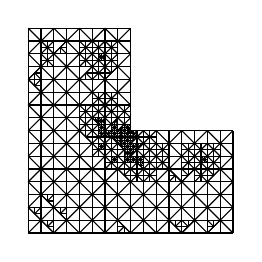
\begin{tikzpicture}[scale = 1.3]
\draw (0.250000,0.000000)  -- (0.250000,-0.125000);
\draw (0.000000,0.250000)  -- (-0.125000,0.250000);
\draw (0.000000,-0.500000)  -- (-0.125000,-0.375000);
\draw (-0.500000,0.000000)  -- (-0.375000,-0.125000);
\draw (-0.125000,0.125000)  -- (-0.062500,0.062500);
\draw (0.125000,-0.125000)  -- (0.062500,-0.062500);
\draw (-0.125000,0.000000)  -- (-0.062500,0.062500);
\draw (0.000000,-0.125000)  -- (0.062500,-0.062500);
\draw (-0.125000,0.125000)  -- (-0.125000,0.062500);
\draw (0.125000,-0.125000)  -- (0.062500,-0.125000);
\draw (-0.125000,0.000000)  -- (-0.125000,0.062500);
\draw (0.000000,-0.125000)  -- (0.062500,-0.125000);
\draw (0.062500,-0.062500)  -- (0.062500,-0.125000);
\draw (-0.062500,0.062500)  -- (-0.125000,0.062500);
\draw (0.000000,0.125000)  -- (-0.062500,0.062500);
\draw (0.125000,0.000000)  -- (0.062500,-0.062500);
\draw (0.125000,-0.125000)  -- (0.125000,-0.062500);
\draw (-0.125000,0.125000)  -- (-0.062500,0.125000);
\draw (0.000000,0.125000)  -- (0.000000,0.062500);
\draw (0.125000,0.000000)  -- (0.062500,0.000000);
\draw (0.125000,0.000000)  -- (0.125000,-0.062500);
\draw (0.000000,0.125000)  -- (-0.062500,0.125000);
\draw (-0.062500,0.062500)  -- (-0.062500,0.125000);
\draw (0.062500,-0.062500)  -- (0.062500,0.000000);
\draw (-0.062500,0.062500)  -- (0.000000,0.062500);
\draw (0.062500,-0.062500)  -- (0.125000,-0.062500);
\draw (0.500000,0.000000)  -- (0.625000,-0.125000);
\draw (0.000000,0.500000)  -- (-0.125000,0.625000);
\draw (-0.250000,0.500000)  -- (-0.125000,0.625000);
\draw (0.500000,0.000000)  -- (0.500000,-0.125000);
\draw (0.000000,0.500000)  -- (-0.125000,0.500000);
\draw (0.500000,-0.250000)  -- (0.500000,-0.125000);
\draw (-0.250000,0.500000)  -- (-0.125000,0.500000);
\draw (-0.125000,0.625000)  -- (-0.125000,0.500000);
\draw (0.625000,-0.125000)  -- (0.500000,-0.125000);
\draw (1.000000,-1.000000)  -- (0.875000,-0.875000);
\draw (-1.000000,1.000000)  -- (-0.875000,0.875000);
\draw (0.500000,-0.500000)  -- (0.625000,-0.375000);
\draw (-0.500000,0.500000)  -- (-0.375000,0.625000);
\draw (-0.500000,1.000000)  -- (-0.375000,0.875000);
\draw (1.000000,-0.500000)  -- (0.875000,-0.375000);
\draw (0.750000,-0.750000)  -- (0.875000,-0.875000);
\draw (-0.062500,-0.062500)  -- (-0.031250,-0.031250);
\draw (-0.062500,0.000000)  -- (-0.031250,-0.031250);
\draw (0.000000,-0.062500)  -- (-0.031250,-0.031250);
\draw (-0.250000,-0.500000)  -- (-0.125000,-0.375000);
\draw (-0.500000,-0.250000)  -- (-0.375000,-0.125000);
\draw (0.750000,-0.500000)  -- (0.875000,-0.375000);
\draw (0.750000,-1.000000)  -- (0.875000,-0.875000);
\draw (-1.000000,0.750000)  -- (-0.875000,0.875000);
\draw (1.000000,-0.750000)  -- (0.875000,-0.875000);
\draw (0.000000,-0.500000)  -- (-0.125000,-0.500000);
\draw (-0.500000,0.000000)  -- (-0.500000,-0.125000);
\draw (-0.250000,-0.250000)  -- (-0.375000,-0.250000);
\draw (-0.250000,-0.250000)  -- (-0.250000,-0.375000);
\draw (0.500000,-0.500000)  -- (0.500000,-0.375000);
\draw (-0.500000,0.500000)  -- (-0.375000,0.500000);
\draw (1.000000,-1.000000)  -- (1.000000,-0.875000);
\draw (-1.000000,1.000000)  -- (-1.000000,0.875000);
\draw (1.000000,-1.000000)  -- (0.875000,-1.000000);
\draw (-0.500000,1.000000)  -- (-0.500000,0.875000);
\draw (1.000000,-0.500000)  -- (0.875000,-0.500000);
\draw (0.750000,-0.750000)  -- (0.750000,-0.875000);
\draw (0.750000,-0.750000)  -- (0.875000,-0.750000);
\draw (-0.062500,-0.062500)  -- (-0.031250,-0.062500);
\draw (-0.062500,-0.062500)  -- (-0.062500,-0.031250);
\draw (-0.250000,-0.500000)  -- (-0.125000,-0.500000);
\draw (-0.500000,-0.250000)  -- (-0.500000,-0.125000);
\draw (-0.500000,-0.250000)  -- (-0.375000,-0.250000);
\draw (-0.250000,-0.500000)  -- (-0.250000,-0.375000);
\draw (0.500000,-0.250000)  -- (0.500000,-0.375000);
\draw (-0.250000,0.500000)  -- (-0.375000,0.500000);
\draw (1.000000,-0.750000)  -- (1.000000,-0.875000);
\draw (-1.000000,0.750000)  -- (-1.000000,0.875000);
\draw (0.750000,-1.000000)  -- (0.875000,-1.000000);
\draw (-0.500000,0.750000)  -- (-0.500000,0.875000);
\draw (0.750000,-0.500000)  -- (0.875000,-0.500000);
\draw (0.750000,-1.000000)  -- (0.750000,-0.875000);
\draw (-1.000000,0.750000)  -- (-0.875000,0.750000);
\draw (1.000000,-0.750000)  -- (0.875000,-0.750000);
\draw (0.000000,-0.062500)  -- (0.000000,-0.031250);
\draw (-0.062500,0.000000)  -- (-0.031250,0.000000);
\draw (0.000000,-0.062500)  -- (-0.031250,-0.062500);
\draw (-0.062500,0.000000)  -- (-0.062500,-0.031250);
\draw (-0.031250,-0.031250)  -- (-0.062500,-0.031250);
\draw (-0.031250,-0.031250)  -- (0.000000,-0.031250);
\draw (-0.125000,-0.375000)  -- (-0.125000,-0.500000);
\draw (-0.375000,-0.125000)  -- (-0.375000,-0.250000);
\draw (0.875000,-0.375000)  -- (0.875000,-0.500000);
\draw (0.875000,-0.875000)  -- (0.875000,-1.000000);
\draw (-0.875000,0.875000)  -- (-0.875000,0.750000);
\draw (0.875000,-0.875000)  -- (0.875000,-0.750000);
\draw (-0.031250,-0.031250)  -- (-0.031250,0.000000);
\draw (-0.031250,-0.031250)  -- (-0.031250,-0.062500);
\draw (-0.125000,-0.375000)  -- (-0.250000,-0.375000);
\draw (-0.375000,-0.125000)  -- (-0.500000,-0.125000);
\draw (0.875000,-0.875000)  -- (0.750000,-0.875000);
\draw (-0.375000,0.875000)  -- (-0.500000,0.875000);
\draw (-0.875000,0.875000)  -- (-1.000000,0.875000);
\draw (0.875000,-0.875000)  -- (1.000000,-0.875000);
\draw (-0.500000,-0.500000)  -- (-0.375000,-0.375000);
\draw (-1.000000,-1.000000)  -- (-0.875000,-0.875000);
\draw (0.500000,-1.000000)  -- (0.625000,-0.875000);
\draw (-1.000000,0.500000)  -- (-0.875000,0.625000);
\draw (-0.500000,1.000000)  -- (-0.625000,0.875000);
\draw (1.000000,-0.500000)  -- (0.875000,-0.625000);
\draw (-0.250000,-0.250000)  -- (-0.312500,-0.187500);
\draw (-1.000000,0.500000)  -- (-0.875000,0.375000);
\draw (0.500000,-1.000000)  -- (0.375000,-0.875000);
\draw (-0.250000,-0.250000)  -- (-0.375000,-0.375000);
\draw (-0.750000,-0.750000)  -- (-0.875000,-0.875000);
\draw (-0.125000,-0.125000)  -- (-0.187500,-0.062500);
\draw (-0.125000,-0.125000)  -- (-0.062500,-0.187500);
\draw (0.750000,-0.750000)  -- (0.625000,-0.875000);
\draw (-0.750000,0.750000)  -- (-0.625000,0.875000);
\draw (0.750000,-0.750000)  -- (0.875000,-0.625000);
\draw (-0.375000,-0.125000)  -- (-0.312500,-0.187500);
\draw (-0.750000,0.250000)  -- (-0.875000,0.375000);
\draw (-0.375000,-0.125000)  -- (-0.312500,-0.062500);
\draw (-0.125000,-0.375000)  -- (-0.062500,-0.312500);
\draw (0.250000,-0.750000)  -- (0.375000,-0.875000);
\draw (-0.375000,0.125000)  -- (-0.312500,0.062500);
\draw (0.125000,-0.375000)  -- (0.062500,-0.312500);
\draw (-0.750000,-1.000000)  -- (-0.875000,-0.875000);
\draw (-1.000000,-0.750000)  -- (-0.875000,-0.875000);
\draw (-0.750000,1.000000)  -- (-0.875000,0.875000);
\draw (-0.250000,-0.125000)  -- (-0.312500,-0.062500);
\draw (-0.375000,0.000000)  -- (-0.312500,-0.062500);
\draw (-0.125000,-0.250000)  -- (-0.062500,-0.312500);
\draw (-0.500000,0.750000)  -- (-0.625000,0.875000);
\draw (-1.000000,0.250000)  -- (-0.875000,0.375000);
\draw (0.000000,-0.375000)  -- (-0.062500,-0.312500);
\draw (-0.250000,-0.500000)  -- (-0.375000,-0.375000);
\draw (-0.500000,-0.250000)  -- (-0.375000,-0.375000);
\draw (0.500000,-0.750000)  -- (0.625000,-0.875000);
\draw (-0.250000,-0.125000)  -- (-0.187500,-0.062500);
\draw (-0.375000,0.000000)  -- (-0.312500,0.062500);
\draw (0.250000,-1.000000)  -- (0.375000,-0.875000);
\draw (-0.125000,-0.250000)  -- (-0.062500,-0.187500);
\draw (0.750000,-0.500000)  -- (0.875000,-0.625000);
\draw (0.000000,-0.375000)  -- (0.062500,-0.312500);
\draw (-0.750000,0.500000)  -- (-0.875000,0.625000);
\draw (-0.500000,-0.500000)  -- (-0.375000,-0.500000);
\draw (-0.500000,-0.500000)  -- (-0.500000,-0.375000);
\draw (-1.000000,-1.000000)  -- (-0.875000,-1.000000);
\draw (-1.000000,-1.000000)  -- (-1.000000,-0.875000);
\draw (-1.000000,1.000000)  -- (-0.875000,1.000000);
\draw (-0.500000,0.500000)  -- (-0.500000,0.625000);
\draw (0.500000,-0.500000)  -- (0.625000,-0.500000);
\draw (-0.250000,-0.250000)  -- (-0.250000,-0.187500);
\draw (-0.250000,0.000000)  -- (-0.187500,0.000000);
\draw (-0.125000,-0.125000)  -- (-0.187500,-0.125000);
\draw (-0.750000,0.750000)  -- (-0.750000,0.625000);
\draw (-0.750000,-0.750000)  -- (-0.875000,-0.750000);
\draw (-0.750000,0.750000)  -- (-0.750000,0.875000);
\draw (0.750000,-0.750000)  -- (0.750000,-0.625000);
\draw (-0.125000,-0.125000)  -- (-0.125000,-0.187500);
\draw (0.750000,-0.750000)  -- (0.625000,-0.750000);
\draw (-0.750000,-0.750000)  -- (-0.750000,-0.875000);
\draw (-0.750000,0.750000)  -- (-0.625000,0.750000);
\draw (-0.250000,0.000000)  -- (-0.250000,0.062500);
\draw (0.000000,-0.250000)  -- (0.062500,-0.250000);
\draw (0.500000,-1.000000)  -- (0.375000,-1.000000);
\draw (-1.000000,0.500000)  -- (-1.000000,0.375000);
\draw (-0.750000,0.250000)  -- (-0.875000,0.250000);
\draw (-0.375000,-0.125000)  -- (-0.375000,-0.062500);
\draw (-0.125000,-0.375000)  -- (-0.125000,-0.312500);
\draw (-0.375000,0.125000)  -- (-0.312500,0.125000);
\draw (0.125000,-0.375000)  -- (0.062500,-0.375000);
\draw (-0.375000,-0.125000)  -- (-0.312500,-0.125000);
\draw (-0.125000,-0.375000)  -- (-0.062500,-0.375000);
\draw (0.250000,-0.750000)  -- (0.250000,-0.875000);
\draw (-0.375000,0.125000)  -- (-0.375000,0.062500);
\draw (0.125000,-0.375000)  -- (0.125000,-0.312500);
\draw (-0.250000,-0.500000)  -- (-0.375000,-0.500000);
\draw (-0.500000,-0.250000)  -- (-0.500000,-0.375000);
\draw (-0.750000,-1.000000)  -- (-0.875000,-1.000000);
\draw (-1.000000,-0.750000)  -- (-1.000000,-0.875000);
\draw (-0.750000,1.000000)  -- (-0.875000,1.000000);
\draw (-0.500000,0.750000)  -- (-0.500000,0.625000);
\draw (0.750000,-0.500000)  -- (0.625000,-0.500000);
\draw (-0.250000,-0.125000)  -- (-0.250000,-0.187500);
\draw (0.500000,-0.750000)  -- (0.500000,-0.875000);
\draw (-0.750000,0.500000)  -- (-0.875000,0.500000);
\draw (-0.125000,-0.250000)  -- (-0.062500,-0.250000);
\draw (-0.250000,-0.125000)  -- (-0.250000,-0.062500);
\draw (-0.250000,-0.125000)  -- (-0.187500,-0.125000);
\draw (-0.750000,0.500000)  -- (-0.750000,0.625000);
\draw (-1.000000,-0.750000)  -- (-0.875000,-0.750000);
\draw (-0.750000,1.000000)  -- (-0.750000,0.875000);
\draw (0.750000,-0.500000)  -- (0.750000,-0.625000);
\draw (-0.125000,-0.250000)  -- (-0.125000,-0.187500);
\draw (0.500000,-0.750000)  -- (0.625000,-0.750000);
\draw (-0.750000,-1.000000)  -- (-0.750000,-0.875000);
\draw (-0.500000,0.750000)  -- (-0.625000,0.750000);
\draw (-0.250000,0.125000)  -- (-0.250000,0.062500);
\draw (0.125000,-0.250000)  -- (0.062500,-0.250000);
\draw (0.250000,-1.000000)  -- (0.375000,-1.000000);
\draw (-1.000000,0.250000)  -- (-1.000000,0.375000);
\draw (0.000000,-0.375000)  -- (0.000000,-0.312500);
\draw (-0.375000,0.000000)  -- (-0.312500,0.000000);
\draw (-1.000000,0.250000)  -- (-0.875000,0.250000);
\draw (-0.375000,0.000000)  -- (-0.375000,-0.062500);
\draw (-0.125000,-0.250000)  -- (-0.125000,-0.312500);
\draw (-0.250000,0.125000)  -- (-0.312500,0.125000);
\draw (0.000000,-0.375000)  -- (0.062500,-0.375000);
\draw (-0.250000,-0.125000)  -- (-0.312500,-0.125000);
\draw (0.000000,-0.375000)  -- (-0.062500,-0.375000);
\draw (0.250000,-1.000000)  -- (0.250000,-0.875000);
\draw (-0.375000,0.000000)  -- (-0.375000,0.062500);
\draw (0.125000,-0.250000)  -- (0.125000,-0.312500);
\draw (-0.875000,-0.875000)  -- (-0.750000,-0.875000);
\draw (-0.875000,-0.875000)  -- (-1.000000,-0.875000);
\draw (-0.375000,0.625000)  -- (-0.500000,0.625000);
\draw (-0.875000,0.875000)  -- (-0.875000,1.000000);
\draw (-0.312500,-0.062500)  -- (-0.250000,-0.062500);
\draw (-0.312500,-0.062500)  -- (-0.375000,-0.062500);
\draw (-0.062500,-0.312500)  -- (-0.125000,-0.312500);
\draw (-0.625000,0.875000)  -- (-0.500000,0.875000);
\draw (-0.875000,0.375000)  -- (-0.875000,0.250000);
\draw (-0.062500,-0.312500)  -- (0.000000,-0.312500);
\draw (-0.375000,-0.375000)  -- (-0.250000,-0.375000);
\draw (-0.375000,-0.375000)  -- (-0.500000,-0.375000);
\draw (0.625000,-0.875000)  -- (0.500000,-0.875000);
\draw (-0.187500,-0.062500)  -- (-0.187500,-0.125000);
\draw (-0.312500,0.062500)  -- (-0.312500,0.000000);
\draw (0.375000,-0.875000)  -- (0.375000,-1.000000);
\draw (-0.062500,-0.187500)  -- (-0.062500,-0.250000);
\draw (0.875000,-0.625000)  -- (0.750000,-0.625000);
\draw (0.062500,-0.312500)  -- (0.062500,-0.375000);
\draw (-0.875000,0.625000)  -- (-0.750000,0.625000);
\draw (-0.312500,-0.187500)  -- (-0.312500,-0.125000);
\draw (-0.875000,-0.875000)  -- (-0.875000,-1.000000);
\draw (-0.875000,-0.875000)  -- (-0.875000,-0.750000);
\draw (0.625000,-0.375000)  -- (0.625000,-0.500000);
\draw (-0.875000,0.875000)  -- (-0.750000,0.875000);
\draw (-0.312500,-0.062500)  -- (-0.312500,-0.125000);
\draw (-0.312500,-0.062500)  -- (-0.312500,0.000000);
\draw (-0.062500,-0.312500)  -- (-0.062500,-0.250000);
\draw (-0.625000,0.875000)  -- (-0.625000,0.750000);
\draw (-0.875000,0.375000)  -- (-1.000000,0.375000);
\draw (-0.062500,-0.312500)  -- (-0.062500,-0.375000);
\draw (-0.375000,-0.375000)  -- (-0.375000,-0.500000);
\draw (-0.375000,-0.375000)  -- (-0.375000,-0.250000);
\draw (0.625000,-0.875000)  -- (0.625000,-0.750000);
\draw (-0.187500,-0.062500)  -- (-0.250000,-0.062500);
\draw (-0.312500,0.062500)  -- (-0.375000,0.062500);
\draw (0.375000,-0.875000)  -- (0.250000,-0.875000);
\draw (-0.062500,-0.187500)  -- (-0.125000,-0.187500);
\draw (0.875000,-0.625000)  -- (0.875000,-0.500000);
\draw (0.062500,-0.312500)  -- (0.000000,-0.312500);
\draw (-0.875000,0.625000)  -- (-0.875000,0.500000);
\draw (-0.312500,-0.187500)  -- (-0.250000,-0.187500);
\draw (1.000000,0.000000)  -- (0.875000,-0.125000);
\draw (0.000000,1.000000)  -- (-0.125000,0.875000);
\draw (0.000000,0.750000)  -- (-0.125000,0.625000);
\draw (0.750000,0.000000)  -- (0.875000,-0.125000);
\draw (0.000000,0.750000)  -- (-0.125000,0.875000);
\draw (-1.000000,0.750000)  -- (-0.875000,0.625000);
\draw (0.750000,0.000000)  -- (0.625000,-0.125000);
\draw (1.000000,-0.250000)  -- (0.875000,-0.375000);
\draw (-0.250000,1.000000)  -- (-0.125000,0.875000);
\draw (1.000000,-0.250000)  -- (0.875000,-0.125000);
\draw (-0.250000,1.000000)  -- (-0.375000,0.875000);
\draw (1.000000,0.000000)  -- (0.875000,0.000000);
\draw (0.000000,1.000000)  -- (0.000000,0.875000);
\draw (-1.000000,0.500000)  -- (-1.000000,0.625000);
\draw (0.500000,0.000000)  -- (0.625000,0.000000);
\draw (0.000000,0.500000)  -- (0.000000,0.625000);
\draw (0.000000,1.000000)  -- (-0.125000,1.000000);
\draw (1.000000,0.000000)  -- (1.000000,-0.125000);
\draw (-0.500000,1.000000)  -- (-0.375000,1.000000);
\draw (1.000000,-0.500000)  -- (1.000000,-0.375000);
\draw (0.750000,0.000000)  -- (0.875000,0.000000);
\draw (0.000000,0.750000)  -- (0.000000,0.875000);
\draw (-1.000000,0.750000)  -- (-1.000000,0.625000);
\draw (0.750000,0.000000)  -- (0.625000,0.000000);
\draw (0.000000,0.750000)  -- (0.000000,0.625000);
\draw (0.000000,0.750000)  -- (-0.125000,0.750000);
\draw (0.750000,0.000000)  -- (0.750000,-0.125000);
\draw (-0.250000,1.000000)  -- (-0.125000,1.000000);
\draw (1.000000,-0.250000)  -- (1.000000,-0.125000);
\draw (-0.250000,1.000000)  -- (-0.375000,1.000000);
\draw (1.000000,-0.250000)  -- (1.000000,-0.375000);
\draw (1.000000,-0.250000)  -- (0.875000,-0.250000);
\draw (-0.250000,1.000000)  -- (-0.250000,0.875000);
\draw (-0.125000,0.625000)  -- (-0.125000,0.750000);
\draw (0.875000,-0.125000)  -- (0.750000,-0.125000);
\draw (-0.125000,0.875000)  -- (0.000000,0.875000);
\draw (-0.875000,0.625000)  -- (-1.000000,0.625000);
\draw (0.625000,-0.125000)  -- (0.625000,0.000000);
\draw (0.875000,-0.375000)  -- (0.875000,-0.250000);
\draw (-0.125000,0.875000)  -- (-0.250000,0.875000);
\draw (0.875000,-0.125000)  -- (1.000000,-0.125000);
\draw (-0.375000,0.875000)  -- (-0.375000,1.000000);
\draw (-0.125000,0.625000)  -- (0.000000,0.625000);
\draw (0.875000,-0.125000)  -- (0.875000,0.000000);
\draw (-0.125000,0.875000)  -- (-0.125000,0.750000);
\draw (-0.875000,0.625000)  -- (-0.875000,0.750000);
\draw (0.625000,-0.125000)  -- (0.750000,-0.125000);
\draw (0.875000,-0.375000)  -- (1.000000,-0.375000);
\draw (-0.125000,0.875000)  -- (-0.125000,1.000000);
\draw (0.875000,-0.125000)  -- (0.875000,-0.250000);
\draw (-0.375000,0.875000)  -- (-0.250000,0.875000);
\draw (0.500000,-0.500000)  -- (0.375000,-0.375000);
\draw (-0.250000,-0.250000)  -- (-0.187500,-0.187500);
\draw (0.000000,-0.250000)  -- (0.062500,-0.187500);
\draw (-0.250000,0.000000)  -- (-0.187500,0.062500);
\draw (-1.000000,0.000000)  -- (-0.875000,0.125000);
\draw (-0.250000,-0.250000)  -- (-0.187500,-0.312500);
\draw (-1.000000,-0.500000)  -- (-0.875000,-0.375000);
\draw (-0.500000,-1.000000)  -- (-0.375000,-0.875000);
\draw (-0.125000,-0.125000)  -- (-0.187500,-0.187500);
\draw (0.125000,-0.125000)  -- (0.062500,-0.187500);
\draw (-0.125000,0.125000)  -- (-0.187500,0.062500);
\draw (-0.750000,0.250000)  -- (-0.875000,0.125000);
\draw (-0.125000,-0.375000)  -- (-0.187500,-0.312500);
\draw (-0.750000,-0.250000)  -- (-0.875000,-0.375000);
\draw (-0.250000,-0.750000)  -- (-0.375000,-0.875000);
\draw (-0.125000,-0.250000)  -- (-0.187500,-0.187500);
\draw (0.500000,-0.250000)  -- (0.375000,-0.375000);
\draw (-0.250000,-0.125000)  -- (-0.187500,-0.187500);
\draw (-0.750000,1.000000)  -- (-0.625000,0.875000);
\draw (-1.000000,0.250000)  -- (-0.875000,0.125000);
\draw (-0.250000,-1.000000)  -- (-0.375000,-0.875000);
\draw (-0.750000,0.500000)  -- (-0.875000,0.375000);
\draw (-1.000000,-0.250000)  -- (-0.875000,-0.375000);
\draw (-0.250000,-0.250000)  -- (-0.187500,-0.250000);
\draw (-0.500000,1.000000)  -- (-0.625000,1.000000);
\draw (-1.000000,0.000000)  -- (-1.000000,0.125000);
\draw (-1.000000,-0.500000)  -- (-1.000000,-0.375000);
\draw (-0.500000,-1.000000)  -- (-0.375000,-1.000000);
\draw (-0.250000,-0.750000)  -- (-0.250000,-0.875000);
\draw (-0.750000,0.250000)  -- (-0.750000,0.375000);
\draw (-0.750000,-0.250000)  -- (-0.875000,-0.250000);
\draw (0.500000,-0.250000)  -- (0.375000,-0.250000);
\draw (-0.125000,-0.250000)  -- (-0.187500,-0.250000);
\draw (-0.750000,1.000000)  -- (-0.625000,1.000000);
\draw (-1.000000,0.250000)  -- (-1.000000,0.125000);
\draw (-1.000000,-0.250000)  -- (-1.000000,-0.375000);
\draw (-0.250000,-1.000000)  -- (-0.375000,-1.000000);
\draw (-0.250000,-1.000000)  -- (-0.250000,-0.875000);
\draw (-0.750000,0.500000)  -- (-0.750000,0.375000);
\draw (-1.000000,-0.250000)  -- (-0.875000,-0.250000);
\draw (-0.187500,-0.187500)  -- (-0.125000,-0.187500);
\draw (0.375000,-0.375000)  -- (0.375000,-0.250000);
\draw (-0.187500,-0.187500)  -- (-0.250000,-0.187500);
\draw (-0.625000,0.875000)  -- (-0.750000,0.875000);
\draw (-0.875000,0.125000)  -- (-1.000000,0.125000);
\draw (-0.375000,-0.875000)  -- (-0.250000,-0.875000);
\draw (-0.187500,-0.312500)  -- (-0.187500,-0.250000);
\draw (-0.875000,0.375000)  -- (-0.875000,0.500000);
\draw (-0.875000,-0.375000)  -- (-1.000000,-0.375000);
\draw (-0.187500,-0.187500)  -- (-0.187500,-0.250000);
\draw (0.375000,-0.375000)  -- (0.500000,-0.375000);
\draw (-0.187500,-0.187500)  -- (-0.187500,-0.125000);
\draw (-0.625000,0.875000)  -- (-0.625000,1.000000);
\draw (-0.875000,0.125000)  -- (-0.875000,0.250000);
\draw (-0.375000,-0.875000)  -- (-0.375000,-1.000000);
\draw (-0.187500,-0.312500)  -- (-0.125000,-0.312500);
\draw (-0.875000,0.375000)  -- (-0.750000,0.375000);
\draw (-0.875000,-0.375000)  -- (-0.875000,-0.250000);
\draw (-0.187500,0.062500)  -- (-0.187500,0.000000);
\draw (-0.500000,0.500000)  -- (-0.375000,0.375000);
\draw (0.000000,0.500000)  -- (-0.125000,0.375000);
\draw (0.500000,0.000000)  -- (0.375000,-0.125000);
\draw (-0.062500,0.062500)  -- (-0.031250,0.031250);
\draw (0.062500,-0.062500)  -- (0.031250,-0.031250);
\draw (-0.500000,0.250000)  -- (-0.375000,0.375000);
\draw (0.250000,-0.500000)  -- (0.375000,-0.375000);
\draw (-0.250000,0.500000)  -- (-0.125000,0.375000);
\draw (0.250000,0.000000)  -- (0.375000,-0.125000);
\draw (-0.250000,0.500000)  -- (-0.375000,0.375000);
\draw (0.000000,0.250000)  -- (-0.125000,0.375000);
\draw (0.500000,-0.250000)  -- (0.375000,-0.125000);
\draw (0.000000,-0.062500)  -- (0.031250,-0.031250);
\draw (-0.062500,0.000000)  -- (-0.031250,0.031250);
\draw (0.000000,0.062500)  -- (-0.031250,0.031250);
\draw (0.062500,0.000000)  -- (0.031250,-0.031250);
\draw (-0.500000,0.500000)  -- (-0.500000,0.375000);
\draw (0.500000,-0.500000)  -- (0.375000,-0.500000);
\draw (-0.500000,0.000000)  -- (-0.500000,0.125000);
\draw (0.000000,-0.500000)  -- (0.125000,-0.500000);
\draw (0.000000,0.500000)  -- (0.000000,0.375000);
\draw (0.500000,0.000000)  -- (0.375000,0.000000);
\draw (-0.062500,0.062500)  -- (-0.062500,0.031250);
\draw (0.062500,-0.062500)  -- (0.031250,-0.062500);
\draw (0.062500,-0.062500)  -- (0.062500,-0.031250);
\draw (-0.062500,0.062500)  -- (-0.031250,0.062500);
\draw (-0.500000,0.250000)  -- (-0.500000,0.375000);
\draw (0.250000,-0.500000)  -- (0.375000,-0.500000);
\draw (-0.500000,0.250000)  -- (-0.500000,0.125000);
\draw (0.250000,-0.500000)  -- (0.125000,-0.500000);
\draw (0.250000,-0.500000)  -- (0.250000,-0.375000);
\draw (-0.500000,0.250000)  -- (-0.375000,0.250000);
\draw (0.000000,0.250000)  -- (0.000000,0.375000);
\draw (0.250000,0.000000)  -- (0.375000,0.000000);
\draw (-0.250000,0.500000)  -- (-0.250000,0.375000);
\draw (-0.062500,0.000000)  -- (-0.062500,0.031250);
\draw (0.000000,-0.062500)  -- (0.031250,-0.062500);
\draw (0.000000,0.062500)  -- (0.000000,0.031250);
\draw (0.062500,0.000000)  -- (0.031250,0.000000);
\draw (0.062500,0.000000)  -- (0.062500,-0.031250);
\draw (0.000000,0.062500)  -- (-0.031250,0.062500);
\draw (-0.375000,0.375000)  -- (-0.375000,0.250000);
\draw (0.375000,-0.375000)  -- (0.375000,-0.500000);
\draw (-0.125000,0.375000)  -- (-0.250000,0.375000);
\draw (0.375000,-0.125000)  -- (0.250000,-0.125000);
\draw (-0.375000,0.375000)  -- (-0.375000,0.500000);
\draw (-0.125000,0.375000)  -- (0.000000,0.375000);
\draw (0.375000,-0.125000)  -- (0.500000,-0.125000);
\draw (0.031250,-0.031250)  -- (0.031250,-0.062500);
\draw (-0.031250,0.031250)  -- (-0.031250,0.000000);
\draw (-0.031250,0.031250)  -- (-0.031250,0.062500);
\draw (0.031250,-0.031250)  -- (0.031250,0.000000);
\draw (-0.375000,0.375000)  -- (-0.500000,0.375000);
\draw (0.375000,-0.375000)  -- (0.250000,-0.375000);
\draw (-0.125000,0.375000)  -- (-0.125000,0.500000);
\draw (0.375000,-0.125000)  -- (0.375000,0.000000);
\draw (-0.375000,0.375000)  -- (-0.250000,0.375000);
\draw (-0.125000,0.375000)  -- (-0.125000,0.250000);
\draw (0.375000,-0.125000)  -- (0.375000,-0.250000);
\draw (0.031250,-0.031250)  -- (0.000000,-0.031250);
\draw (-0.031250,0.031250)  -- (-0.062500,0.031250);
\draw (-0.031250,0.031250)  -- (0.000000,0.031250);
\draw (0.031250,-0.031250)  -- (0.062500,-0.031250);
\draw (-1.000000,-0.500000)  -- (-0.875000,-0.625000);
\draw (-0.500000,-1.000000)  -- (-0.625000,-0.875000);
\draw (0.000000,-1.000000)  -- (0.125000,-0.875000);
\draw (-1.000000,0.000000)  -- (-0.875000,-0.125000);
\draw (0.250000,-0.250000)  -- (0.187500,-0.312500);
\draw (-0.250000,0.250000)  -- (-0.312500,0.187500);
\draw (-0.750000,-0.750000)  -- (-0.875000,-0.625000);
\draw (-0.750000,-0.750000)  -- (-0.625000,-0.875000);
\draw (0.250000,-0.750000)  -- (0.125000,-0.875000);
\draw (-0.750000,-0.250000)  -- (-0.875000,-0.125000);
\draw (0.125000,-0.375000)  -- (0.187500,-0.312500);
\draw (-0.375000,0.125000)  -- (-0.312500,0.187500);
\draw (0.625000,-0.375000)  -- (0.687500,-0.312500);
\draw (-0.375000,0.625000)  -- (-0.312500,0.687500);
\draw (0.500000,-0.750000)  -- (0.375000,-0.875000);
\draw (-0.750000,-0.500000)  -- (-0.875000,-0.625000);
\draw (-1.000000,-0.250000)  -- (-0.875000,-0.125000);
\draw (0.750000,-1.000000)  -- (0.625000,-0.875000);
\draw (0.750000,-0.375000)  -- (0.687500,-0.312500);
\draw (0.625000,-0.250000)  -- (0.687500,-0.312500);
\draw (0.250000,-1.000000)  -- (0.125000,-0.875000);
\draw (-0.500000,-0.750000)  -- (-0.625000,-0.875000);
\draw (-0.250000,0.625000)  -- (-0.312500,0.687500);
\draw (-0.375000,0.750000)  -- (-0.312500,0.687500);
\draw (0.125000,-0.250000)  -- (0.187500,-0.312500);
\draw (-0.250000,0.125000)  -- (-0.312500,0.187500);
\draw (-0.750000,-0.500000)  -- (-0.875000,-0.375000);
\draw (0.500000,-1.000000)  -- (0.625000,-1.000000);
\draw (-1.000000,-0.500000)  -- (-0.875000,-0.500000);
\draw (-0.500000,-1.000000)  -- (-0.500000,-0.875000);
\draw (-0.750000,-0.750000)  -- (-0.625000,-0.750000);
\draw (-0.750000,-0.750000)  -- (-0.750000,-0.625000);
\draw (-0.250000,0.250000)  -- (-0.250000,0.187500);
\draw (0.250000,-0.250000)  -- (0.187500,-0.250000);
\draw (0.000000,-1.000000)  -- (0.125000,-1.000000);
\draw (-1.000000,0.000000)  -- (-1.000000,-0.125000);
\draw (0.250000,-0.750000)  -- (0.375000,-0.750000);
\draw (-0.750000,-0.250000)  -- (-0.750000,-0.375000);
\draw (0.750000,-0.250000)  -- (0.687500,-0.250000);
\draw (-0.250000,0.750000)  -- (-0.250000,0.687500);
\draw (-0.250000,0.750000)  -- (-0.312500,0.750000);
\draw (0.750000,-0.250000)  -- (0.750000,-0.312500);
\draw (-0.375000,0.625000)  -- (-0.312500,0.625000);
\draw (0.625000,-0.375000)  -- (0.625000,-0.312500);
\draw (0.625000,-0.375000)  -- (0.687500,-0.375000);
\draw (-0.375000,0.625000)  -- (-0.375000,0.687500);
\draw (0.750000,-1.000000)  -- (0.625000,-1.000000);
\draw (-0.750000,-0.500000)  -- (-0.875000,-0.500000);
\draw (-0.500000,-0.750000)  -- (-0.500000,-0.875000);
\draw (-0.500000,-0.750000)  -- (-0.625000,-0.750000);
\draw (-0.750000,-0.500000)  -- (-0.750000,-0.625000);
\draw (-0.250000,0.125000)  -- (-0.250000,0.187500);
\draw (0.125000,-0.250000)  -- (0.187500,-0.250000);
\draw (0.250000,-1.000000)  -- (0.125000,-1.000000);
\draw (-1.000000,-0.250000)  -- (-1.000000,-0.125000);
\draw (0.500000,-0.750000)  -- (0.375000,-0.750000);
\draw (-0.750000,-0.500000)  -- (-0.750000,-0.375000);
\draw (0.625000,-0.250000)  -- (0.687500,-0.250000);
\draw (-0.250000,0.625000)  -- (-0.250000,0.687500);
\draw (-0.375000,0.750000)  -- (-0.312500,0.750000);
\draw (0.750000,-0.375000)  -- (0.750000,-0.312500);
\draw (-0.250000,0.625000)  -- (-0.312500,0.625000);
\draw (0.625000,-0.250000)  -- (0.625000,-0.312500);
\draw (0.750000,-0.375000)  -- (0.687500,-0.375000);
\draw (-0.375000,0.750000)  -- (-0.375000,0.687500);
\draw (0.375000,-0.875000)  -- (0.375000,-0.750000);
\draw (-0.875000,-0.625000)  -- (-0.875000,-0.500000);
\draw (-0.875000,-0.125000)  -- (-0.875000,-0.250000);
\draw (0.625000,-0.875000)  -- (0.750000,-0.875000);
\draw (0.687500,-0.312500)  -- (0.750000,-0.312500);
\draw (0.687500,-0.312500)  -- (0.625000,-0.312500);
\draw (0.125000,-0.875000)  -- (0.250000,-0.875000);
\draw (-0.625000,-0.875000)  -- (-0.625000,-0.750000);
\draw (-0.312500,0.687500)  -- (-0.250000,0.687500);
\draw (-0.312500,0.687500)  -- (-0.375000,0.687500);
\draw (0.187500,-0.312500)  -- (0.125000,-0.312500);
\draw (-0.312500,0.187500)  -- (-0.250000,0.187500);
\draw (-0.875000,-0.375000)  -- (-0.750000,-0.375000);
\draw (0.375000,-0.875000)  -- (0.500000,-0.875000);
\draw (-0.875000,-0.625000)  -- (-0.750000,-0.625000);
\draw (-0.875000,-0.125000)  -- (-1.000000,-0.125000);
\draw (0.625000,-0.875000)  -- (0.625000,-1.000000);
\draw (0.687500,-0.312500)  -- (0.687500,-0.375000);
\draw (0.687500,-0.312500)  -- (0.687500,-0.250000);
\draw (0.125000,-0.875000)  -- (0.125000,-1.000000);
\draw (-0.625000,-0.875000)  -- (-0.500000,-0.875000);
\draw (-0.312500,0.687500)  -- (-0.312500,0.625000);
\draw (-0.312500,0.687500)  -- (-0.312500,0.750000);
\draw (0.187500,-0.312500)  -- (0.187500,-0.250000);
\draw (-0.312500,0.187500)  -- (-0.312500,0.125000);
\draw (-0.875000,-0.375000)  -- (-0.875000,-0.500000);
\draw (0.000000,0.000000)  -- (-0.015625,-0.015625);
\draw (-0.031250,-0.031250)  -- (-0.015625,-0.015625);
\draw (1.000000,-0.750000)  -- (0.875000,-0.625000);
\draw (-0.500000,-0.750000)  -- (-0.375000,-0.875000);
\draw (0.000000,-0.031250)  -- (-0.015625,-0.015625);
\draw (-0.031250,0.000000)  -- (-0.015625,-0.015625);
\draw (1.000000,-0.500000)  -- (1.000000,-0.625000);
\draw (-0.250000,-0.750000)  -- (-0.375000,-0.750000);
\draw (0.000000,0.000000)  -- (0.000000,-0.015625);
\draw (0.000000,0.000000)  -- (-0.015625,0.000000);
\draw (-0.031250,-0.031250)  -- (-0.015625,-0.031250);
\draw (-0.031250,-0.031250)  -- (-0.031250,-0.015625);
\draw (1.000000,-0.750000)  -- (1.000000,-0.625000);
\draw (-0.500000,-0.750000)  -- (-0.375000,-0.750000);
\draw (0.000000,-0.031250)  -- (0.000000,-0.015625);
\draw (-0.031250,0.000000)  -- (-0.015625,0.000000);
\draw (0.000000,-0.031250)  -- (-0.015625,-0.031250);
\draw (-0.031250,0.000000)  -- (-0.031250,-0.015625);
\draw (0.875000,-0.625000)  -- (1.000000,-0.625000);
\draw (-0.375000,-0.875000)  -- (-0.500000,-0.875000);
\draw (-0.015625,-0.015625)  -- (0.000000,-0.015625);
\draw (-0.015625,-0.015625)  -- (-0.031250,-0.015625);
\draw (0.875000,-0.625000)  -- (0.875000,-0.750000);
\draw (-0.375000,-0.875000)  -- (-0.375000,-0.750000);
\draw (-0.015625,-0.015625)  -- (-0.015625,-0.031250);
\draw (-0.015625,-0.015625)  -- (-0.015625,0.000000);
\draw (-0.125000,-0.125000)  -- (-0.093750,-0.093750);
\draw (0.000000,-0.125000)  -- (-0.031250,-0.093750);
\draw (-0.125000,0.000000)  -- (-0.093750,-0.031250);
\draw (0.000000,-1.000000)  -- (-0.125000,-0.875000);
\draw (0.000000,-0.500000)  -- (-0.062500,-0.437500);
\draw (-0.500000,0.000000)  -- (-0.437500,-0.062500);
\draw (0.000000,-0.500000)  -- (0.062500,-0.437500);
\draw (-0.500000,0.000000)  -- (-0.437500,0.062500);
\draw (0.750000,-0.250000)  -- (0.687500,-0.187500);
\draw (-0.250000,0.750000)  -- (-0.187500,0.687500);
\draw (0.500000,-0.250000)  -- (0.562500,-0.187500);
\draw (-0.250000,0.500000)  -- (-0.187500,0.562500);
\draw (-0.750000,0.750000)  -- (-0.812500,0.812500);
\draw (-0.250000,0.750000)  -- (-0.312500,0.812500);
\draw (0.750000,-0.250000)  -- (0.812500,-0.312500);
\draw (0.500000,-0.250000)  -- (0.562500,-0.312500);
\draw (-0.250000,0.500000)  -- (-0.312500,0.562500);
\draw (-0.250000,0.000000)  -- (-0.281250,-0.031250);
\draw (0.000000,-0.250000)  -- (-0.031250,-0.281250);
\draw (-0.250000,0.000000)  -- (-0.281250,0.031250);
\draw (0.000000,-0.250000)  -- (0.031250,-0.281250);
\draw (-0.125000,-0.125000)  -- (-0.156250,-0.093750);
\draw (-0.125000,-0.125000)  -- (-0.093750,-0.156250);
\draw (-0.125000,0.000000)  -- (-0.156250,-0.031250);
\draw (0.000000,-0.125000)  -- (-0.031250,-0.156250);
\draw (-0.750000,-1.000000)  -- (-0.812500,-0.937500);
\draw (-1.000000,-0.750000)  -- (-0.937500,-0.812500);
\draw (0.000000,-0.125000)  -- (0.031250,-0.156250);
\draw (-0.125000,0.000000)  -- (-0.156250,0.031250);
\draw (-0.062500,-0.062500)  -- (-0.093750,-0.093750);
\draw (-0.062500,-0.062500)  -- (-0.031250,-0.093750);
\draw (-0.062500,-0.062500)  -- (-0.093750,-0.031250);
\draw (-0.250000,-0.750000)  -- (-0.125000,-0.875000);
\draw (-0.125000,-0.375000)  -- (-0.062500,-0.437500);
\draw (-0.375000,-0.125000)  -- (-0.437500,-0.062500);
\draw (0.125000,-0.375000)  -- (0.062500,-0.437500);
\draw (-0.375000,0.125000)  -- (-0.437500,0.062500);
\draw (0.625000,-0.125000)  -- (0.687500,-0.187500);
\draw (-0.125000,0.625000)  -- (-0.187500,0.687500);
\draw (0.625000,-0.125000)  -- (0.562500,-0.187500);
\draw (-0.125000,0.625000)  -- (-0.187500,0.562500);
\draw (-0.875000,0.875000)  -- (-0.812500,0.812500);
\draw (-0.375000,0.875000)  -- (-0.312500,0.812500);
\draw (0.875000,-0.375000)  -- (0.812500,-0.312500);
\draw (0.625000,-0.375000)  -- (0.562500,-0.312500);
\draw (-0.375000,0.625000)  -- (-0.312500,0.562500);
\draw (-0.312500,-0.062500)  -- (-0.281250,-0.031250);
\draw (-0.062500,-0.312500)  -- (-0.031250,-0.281250);
\draw (-0.312500,0.062500)  -- (-0.281250,0.031250);
\draw (0.062500,-0.312500)  -- (0.031250,-0.281250);
\draw (-0.187500,-0.062500)  -- (-0.156250,-0.093750);
\draw (-0.062500,-0.187500)  -- (-0.093750,-0.156250);
\draw (-0.187500,-0.062500)  -- (-0.156250,-0.031250);
\draw (-0.062500,-0.187500)  -- (-0.031250,-0.156250);
\draw (-0.875000,-0.875000)  -- (-0.812500,-0.937500);
\draw (-0.875000,-0.875000)  -- (-0.937500,-0.812500);
\draw (0.062500,-0.187500)  -- (0.031250,-0.156250);
\draw (-0.187500,0.062500)  -- (-0.156250,0.031250);
\draw (-0.250000,-1.000000)  -- (-0.125000,-0.875000);
\draw (-0.750000,-1.000000)  -- (-0.625000,-0.875000);
\draw (-0.125000,-0.062500)  -- (-0.156250,-0.031250);
\draw (-0.375000,-0.250000)  -- (-0.312500,-0.187500);
\draw (-0.062500,-0.125000)  -- (-0.031250,-0.156250);
\draw (-0.312500,0.000000)  -- (-0.281250,-0.031250);
\draw (-0.187500,0.000000)  -- (-0.156250,-0.031250);
\draw (0.000000,-0.187500)  -- (-0.031250,-0.156250);
\draw (-0.250000,-0.375000)  -- (-0.187500,-0.312500);
\draw (0.625000,-0.250000)  -- (0.687500,-0.187500);
\draw (-0.062500,0.000000)  -- (-0.093750,-0.031250);
\draw (0.625000,-0.250000)  -- (0.562500,-0.312500);
\draw (0.000000,-0.312500)  -- (-0.031250,-0.281250);
\draw (0.000000,-0.062500)  -- (-0.031250,-0.093750);
\draw (-0.250000,0.625000)  -- (-0.312500,0.562500);
\draw (-0.250000,-0.062500)  -- (-0.281250,-0.031250);
\draw (-0.750000,0.000000)  -- (-0.875000,0.125000);
\draw (-0.250000,0.625000)  -- (-0.187500,0.687500);
\draw (-0.062500,-0.250000)  -- (-0.031250,-0.281250);
\draw (-0.312500,0.000000)  -- (-0.281250,0.031250);
\draw (0.750000,-0.375000)  -- (0.812500,-0.312500);
\draw (-1.000000,-0.750000)  -- (-0.875000,-0.625000);
\draw (-0.375000,0.750000)  -- (-0.312500,0.812500);
\draw (0.625000,-0.250000)  -- (0.562500,-0.187500);
\draw (0.000000,-0.312500)  -- (0.031250,-0.281250);
\draw (-0.375000,0.000000)  -- (-0.437500,0.062500);
\draw (-0.250000,0.625000)  -- (-0.187500,0.562500);
\draw (0.000000,-0.187500)  -- (0.031250,-0.156250);
\draw (-0.062500,-0.125000)  -- (-0.031250,-0.093750);
\draw (-0.125000,-0.062500)  -- (-0.093750,-0.031250);
\draw (-0.750000,0.875000)  -- (-0.812500,0.812500);
\draw (-0.125000,-0.062500)  -- (-0.156250,-0.093750);
\draw (-0.375000,0.000000)  -- (-0.437500,-0.062500);
\draw (-0.187500,0.000000)  -- (-0.156250,0.031250);
\draw (-0.750000,-0.875000)  -- (-0.812500,-0.937500);
\draw (-0.875000,-0.750000)  -- (-0.937500,-0.812500);
\draw (-0.875000,0.750000)  -- (-0.812500,0.812500);
\draw (0.000000,-0.375000)  -- (-0.062500,-0.437500);
\draw (-0.062500,-0.125000)  -- (-0.093750,-0.156250);
\draw (-0.125000,-0.062500)  -- (-0.093750,-0.093750);
\draw (-0.062500,-0.125000)  -- (-0.093750,-0.093750);
\draw (0.000000,-0.375000)  -- (0.062500,-0.437500);
\draw (0.000000,-0.750000)  -- (0.125000,-0.875000);
\draw (-0.500000,-1.000000)  -- (-0.625000,-1.000000);
\draw (-1.000000,-0.500000)  -- (-1.000000,-0.625000);
\draw (-0.125000,-0.125000)  -- (-0.093750,-0.125000);
\draw (-0.125000,-0.125000)  -- (-0.125000,-0.093750);
\draw (0.000000,-0.125000)  -- (0.000000,-0.093750);
\draw (-0.125000,0.000000)  -- (-0.093750,0.000000);
\draw (0.000000,-0.125000)  -- (-0.031250,-0.125000);
\draw (-0.125000,0.000000)  -- (-0.125000,-0.031250);
\draw (-0.062500,-0.062500)  -- (-0.093750,-0.062500);
\draw (-0.062500,-0.062500)  -- (-0.062500,-0.093750);
\draw (0.000000,-0.500000)  -- (0.000000,-0.437500);
\draw (-0.500000,0.000000)  -- (-0.437500,0.000000);
\draw (0.000000,-1.000000)  -- (0.000000,-0.875000);
\draw (-1.000000,0.000000)  -- (-0.875000,0.000000);
\draw (0.250000,-0.750000)  -- (0.125000,-0.750000);
\draw (-0.750000,0.250000)  -- (-0.750000,0.125000);
\draw (0.500000,-0.250000)  -- (0.562500,-0.250000);
\draw (-0.250000,0.500000)  -- (-0.250000,0.562500);
\draw (0.625000,-0.125000)  -- (0.625000,-0.187500);
\draw (-0.125000,0.625000)  -- (-0.187500,0.625000);
\draw (-0.250000,-0.250000)  -- (-0.312500,-0.250000);
\draw (-0.250000,-0.250000)  -- (-0.250000,-0.312500);
\draw (-0.750000,0.750000)  -- (-0.812500,0.750000);
\draw (-0.375000,-0.125000)  -- (-0.375000,-0.187500);
\draw (-0.375000,0.875000)  -- (-0.375000,0.812500);
\draw (-0.875000,0.875000)  -- (-0.875000,0.812500);
\draw (-0.125000,-0.375000)  -- (-0.187500,-0.375000);
\draw (0.875000,-0.375000)  -- (0.812500,-0.375000);
\draw (0.000000,-0.250000)  -- (-0.031250,-0.250000);
\draw (-0.250000,0.000000)  -- (-0.250000,-0.031250);
\draw (-0.750000,0.750000)  -- (-0.750000,0.812500);
\draw (0.000000,-0.250000)  -- (0.000000,-0.281250);
\draw (-0.250000,0.000000)  -- (-0.281250,0.000000);
\draw (0.000000,-0.125000)  -- (0.000000,-0.156250);
\draw (-0.125000,0.000000)  -- (-0.156250,0.000000);
\draw (-1.000000,-0.750000)  -- (-0.937500,-0.750000);
\draw (-0.750000,-1.000000)  -- (-0.750000,-0.937500);
\draw (-0.187500,-0.062500)  -- (-0.187500,-0.031250);
\draw (-0.062500,-0.187500)  -- (-0.062500,-0.156250);
\draw (-0.875000,-0.875000)  -- (-0.812500,-0.875000);
\draw (-0.312500,-0.062500)  -- (-0.281250,-0.062500);
\draw (-0.062500,-0.312500)  -- (-0.031250,-0.312500);
\draw (-0.312500,0.062500)  -- (-0.312500,0.031250);
\draw (-0.187500,-0.062500)  -- (-0.156250,-0.062500);
\draw (-0.062500,-0.187500)  -- (-0.031250,-0.187500);
\draw (-0.875000,-0.875000)  -- (-0.875000,-0.812500);
\draw (-0.875000,0.875000)  -- (-0.812500,0.875000);
\draw (-0.312500,-0.062500)  -- (-0.312500,-0.031250);
\draw (-0.062500,-0.312500)  -- (-0.062500,-0.281250);
\draw (0.062500,-0.312500)  -- (0.031250,-0.312500);
\draw (0.062500,-0.187500)  -- (0.031250,-0.187500);
\draw (-0.187500,0.062500)  -- (-0.187500,0.031250);
\draw (-0.750000,-1.000000)  -- (-0.625000,-1.000000);
\draw (-1.000000,-0.750000)  -- (-1.000000,-0.625000);
\draw (-0.062500,-0.125000)  -- (-0.093750,-0.125000);
\draw (-0.125000,-0.062500)  -- (-0.125000,-0.093750);
\draw (0.000000,-0.062500)  -- (0.000000,-0.093750);
\draw (-0.062500,0.000000)  -- (-0.093750,0.000000);
\draw (-0.062500,-0.125000)  -- (-0.031250,-0.125000);
\draw (-0.125000,-0.062500)  -- (-0.125000,-0.031250);
\draw (-0.125000,-0.062500)  -- (-0.093750,-0.062500);
\draw (-0.062500,-0.125000)  -- (-0.062500,-0.093750);
\draw (-0.250000,-1.000000)  -- (-0.125000,-1.000000);
\draw (0.000000,-0.375000)  -- (0.000000,-0.437500);
\draw (-0.375000,0.000000)  -- (-0.437500,0.000000);
\draw (0.000000,-0.750000)  -- (0.000000,-0.875000);
\draw (-0.750000,0.000000)  -- (-0.875000,0.000000);
\draw (0.000000,-0.750000)  -- (0.125000,-0.750000);
\draw (-0.750000,0.000000)  -- (-0.750000,0.125000);
\draw (0.625000,-0.250000)  -- (0.562500,-0.250000);
\draw (-0.250000,0.625000)  -- (-0.250000,0.562500);
\draw (0.625000,-0.250000)  -- (0.625000,-0.187500);
\draw (-0.250000,0.625000)  -- (-0.187500,0.625000);
\draw (-0.375000,-0.250000)  -- (-0.312500,-0.250000);
\draw (-0.250000,-0.375000)  -- (-0.250000,-0.312500);
\draw (-0.875000,0.750000)  -- (-0.812500,0.750000);
\draw (-0.375000,-0.250000)  -- (-0.375000,-0.187500);
\draw (-0.375000,0.750000)  -- (-0.375000,0.812500);
\draw (-0.875000,0.750000)  -- (-0.875000,0.812500);
\draw (-0.250000,-0.375000)  -- (-0.187500,-0.375000);
\draw (0.750000,-0.375000)  -- (0.812500,-0.375000);
\draw (-0.062500,-0.250000)  -- (-0.031250,-0.250000);
\draw (-0.250000,-0.062500)  -- (-0.250000,-0.031250);
\draw (-0.750000,0.875000)  -- (-0.750000,0.812500);
\draw (0.000000,-0.312500)  -- (0.000000,-0.281250);
\draw (-0.312500,0.000000)  -- (-0.281250,0.000000);
\draw (0.000000,-0.187500)  -- (0.000000,-0.156250);
\draw (-0.187500,0.000000)  -- (-0.156250,0.000000);
\draw (-0.875000,-0.750000)  -- (-0.937500,-0.750000);
\draw (-0.750000,-0.875000)  -- (-0.750000,-0.937500);
\draw (-0.187500,0.000000)  -- (-0.187500,-0.031250);
\draw (-0.062500,-0.125000)  -- (-0.062500,-0.156250);
\draw (-0.750000,-0.875000)  -- (-0.812500,-0.875000);
\draw (-0.250000,-0.062500)  -- (-0.281250,-0.062500);
\draw (0.000000,-0.312500)  -- (-0.031250,-0.312500);
\draw (-0.312500,0.000000)  -- (-0.312500,0.031250);
\draw (-0.125000,-0.062500)  -- (-0.156250,-0.062500);
\draw (0.000000,-0.187500)  -- (-0.031250,-0.187500);
\draw (-0.875000,-0.750000)  -- (-0.875000,-0.812500);
\draw (-0.750000,0.875000)  -- (-0.812500,0.875000);
\draw (-0.312500,0.000000)  -- (-0.312500,-0.031250);
\draw (-0.062500,-0.250000)  -- (-0.062500,-0.281250);
\draw (0.000000,-0.312500)  -- (0.031250,-0.312500);
\draw (0.000000,-0.187500)  -- (0.031250,-0.187500);
\draw (-0.187500,0.000000)  -- (-0.187500,0.031250);
\draw (-0.125000,-0.875000)  -- (-0.125000,-1.000000);
\draw (-0.625000,-0.875000)  -- (-0.625000,-1.000000);
\draw (-0.156250,-0.031250)  -- (-0.125000,-0.031250);
\draw (-0.312500,-0.187500)  -- (-0.312500,-0.250000);
\draw (-0.031250,-0.156250)  -- (-0.062500,-0.156250);
\draw (-0.281250,-0.031250)  -- (-0.312500,-0.031250);
\draw (-0.156250,-0.031250)  -- (-0.187500,-0.031250);
\draw (-0.031250,-0.156250)  -- (0.000000,-0.156250);
\draw (-0.187500,-0.312500)  -- (-0.187500,-0.375000);
\draw (0.687500,-0.187500)  -- (0.687500,-0.250000);
\draw (-0.093750,-0.031250)  -- (-0.093750,0.000000);
\draw (0.562500,-0.312500)  -- (0.562500,-0.250000);
\draw (-0.031250,-0.281250)  -- (0.000000,-0.281250);
\draw (-0.031250,-0.093750)  -- (-0.031250,-0.062500);
\draw (-0.312500,0.562500)  -- (-0.312500,0.625000);
\draw (-0.281250,-0.031250)  -- (-0.250000,-0.031250);
\draw (-0.875000,0.125000)  -- (-0.750000,0.125000);
\draw (-0.187500,0.687500)  -- (-0.187500,0.625000);
\draw (-0.031250,-0.281250)  -- (-0.062500,-0.281250);
\draw (-0.281250,0.031250)  -- (-0.281250,0.000000);
\draw (0.812500,-0.312500)  -- (0.812500,-0.375000);
\draw (-0.875000,-0.625000)  -- (-0.875000,-0.750000);
\draw (-0.312500,0.812500)  -- (-0.312500,0.750000);
\draw (0.562500,-0.187500)  -- (0.625000,-0.187500);
\draw (0.031250,-0.281250)  -- (0.031250,-0.312500);
\draw (-0.437500,0.062500)  -- (-0.375000,0.062500);
\draw (-0.187500,0.562500)  -- (-0.250000,0.562500);
\draw (0.031250,-0.156250)  -- (0.031250,-0.187500);
\draw (-0.031250,-0.093750)  -- (-0.031250,-0.125000);
\draw (-0.093750,-0.031250)  -- (-0.093750,-0.062500);
\draw (-0.812500,0.812500)  -- (-0.812500,0.875000);
\draw (-0.156250,-0.093750)  -- (-0.156250,-0.062500);
\draw (-0.437500,-0.062500)  -- (-0.437500,0.000000);
\draw (-0.156250,0.031250)  -- (-0.156250,0.000000);
\draw (-0.812500,-0.937500)  -- (-0.812500,-0.875000);
\draw (-0.937500,-0.812500)  -- (-0.937500,-0.750000);
\draw (-0.812500,0.812500)  -- (-0.812500,0.750000);
\draw (-0.062500,-0.437500)  -- (-0.062500,-0.375000);
\draw (-0.093750,-0.156250)  -- (-0.093750,-0.125000);
\draw (-0.093750,-0.093750)  -- (-0.125000,-0.093750);
\draw (-0.093750,-0.093750)  -- (-0.062500,-0.093750);
\draw (0.062500,-0.437500)  -- (0.000000,-0.437500);
\draw (0.125000,-0.875000)  -- (0.000000,-0.875000);
\draw (-0.125000,-0.875000)  -- (-0.250000,-0.875000);
\draw (-0.625000,-0.875000)  -- (-0.750000,-0.875000);
\draw (-0.156250,-0.031250)  -- (-0.156250,-0.062500);
\draw (-0.312500,-0.187500)  -- (-0.375000,-0.187500);
\draw (-0.031250,-0.156250)  -- (-0.031250,-0.125000);
\draw (-0.281250,-0.031250)  -- (-0.281250,0.000000);
\draw (-0.156250,-0.031250)  -- (-0.156250,0.000000);
\draw (-0.031250,-0.156250)  -- (-0.031250,-0.187500);
\draw (-0.187500,-0.312500)  -- (-0.250000,-0.312500);
\draw (0.687500,-0.187500)  -- (0.625000,-0.187500);
\draw (-0.093750,-0.031250)  -- (-0.062500,-0.031250);
\draw (0.562500,-0.312500)  -- (0.625000,-0.312500);
\draw (-0.031250,-0.281250)  -- (-0.031250,-0.312500);
\draw (-0.031250,-0.093750)  -- (0.000000,-0.093750);
\draw (-0.312500,0.562500)  -- (-0.250000,0.562500);
\draw (-0.281250,-0.031250)  -- (-0.281250,-0.062500);
\draw (-0.875000,0.125000)  -- (-0.875000,0.000000);
\draw (-0.187500,0.687500)  -- (-0.250000,0.687500);
\draw (-0.031250,-0.281250)  -- (-0.031250,-0.250000);
\draw (-0.281250,0.031250)  -- (-0.312500,0.031250);
\draw (0.812500,-0.312500)  -- (0.750000,-0.312500);
\draw (-0.875000,-0.625000)  -- (-1.000000,-0.625000);
\draw (-0.312500,0.812500)  -- (-0.375000,0.812500);
\draw (0.562500,-0.187500)  -- (0.562500,-0.250000);
\draw (0.031250,-0.281250)  -- (0.000000,-0.281250);
\draw (-0.437500,0.062500)  -- (-0.437500,0.000000);
\draw (-0.187500,0.562500)  -- (-0.187500,0.625000);
\draw (0.031250,-0.156250)  -- (0.000000,-0.156250);
\draw (-0.031250,-0.093750)  -- (-0.062500,-0.093750);
\draw (-0.093750,-0.031250)  -- (-0.125000,-0.031250);
\draw (-0.812500,0.812500)  -- (-0.750000,0.812500);
\draw (-0.156250,-0.093750)  -- (-0.125000,-0.093750);
\draw (-0.437500,-0.062500)  -- (-0.375000,-0.062500);
\draw (-0.156250,0.031250)  -- (-0.187500,0.031250);
\draw (-0.812500,-0.937500)  -- (-0.750000,-0.937500);
\draw (-0.937500,-0.812500)  -- (-0.875000,-0.812500);
\draw (-0.812500,0.812500)  -- (-0.875000,0.812500);
\draw (-0.062500,-0.437500)  -- (0.000000,-0.437500);
\draw (-0.093750,-0.156250)  -- (-0.062500,-0.156250);
\draw (-0.093750,-0.093750)  -- (-0.093750,-0.062500);
\draw (-0.093750,-0.093750)  -- (-0.093750,-0.125000);
\draw (0.062500,-0.437500)  -- (0.062500,-0.375000);
\draw (0.125000,-0.875000)  -- (0.125000,-0.750000);
\draw (0.500000,-0.500000)  -- (0.625000,-0.625000);
\draw (-0.500000,-0.500000)  -- (-0.625000,-0.625000);
\draw (-0.500000,0.500000)  -- (-0.625000,0.625000);
\draw (-0.250000,0.250000)  -- (-0.187500,0.187500);
\draw (0.250000,-0.250000)  -- (0.187500,-0.187500);
\draw (-0.500000,-0.500000)  -- (-0.375000,-0.625000);
\draw (0.500000,-0.500000)  -- (0.375000,-0.625000);
\draw (-0.500000,-0.500000)  -- (-0.625000,-0.375000);
\draw (-0.500000,0.500000)  -- (-0.625000,0.375000);
\draw (0.000000,-0.500000)  -- (-0.125000,-0.625000);
\draw (-0.500000,0.000000)  -- (-0.625000,0.125000);
\draw (0.000000,-0.500000)  -- (0.125000,-0.625000);
\draw (-0.500000,0.000000)  -- (-0.625000,-0.125000);
\draw (0.750000,-0.750000)  -- (0.625000,-0.625000);
\draw (-0.750000,-0.750000)  -- (-0.625000,-0.625000);
\draw (-0.750000,0.750000)  -- (-0.625000,0.625000);
\draw (-0.125000,0.125000)  -- (-0.187500,0.187500);
\draw (0.125000,-0.125000)  -- (0.187500,-0.187500);
\draw (-0.250000,-0.750000)  -- (-0.375000,-0.625000);
\draw (0.250000,-0.750000)  -- (0.375000,-0.625000);
\draw (-0.750000,-0.250000)  -- (-0.625000,-0.375000);
\draw (-0.750000,0.250000)  -- (-0.625000,0.375000);
\draw (-0.250000,-0.750000)  -- (-0.125000,-0.625000);
\draw (-0.750000,0.250000)  -- (-0.625000,0.125000);
\draw (0.250000,-0.750000)  -- (0.125000,-0.625000);
\draw (-0.750000,-0.250000)  -- (-0.625000,-0.125000);
\draw (0.500000,-0.750000)  -- (0.625000,-0.625000);
\draw (-0.750000,-0.500000)  -- (-0.625000,-0.625000);
\draw (-0.500000,0.750000)  -- (-0.625000,0.625000);
\draw (-0.750000,0.500000)  -- (-0.625000,0.625000);
\draw (-0.500000,-0.750000)  -- (-0.625000,-0.625000);
\draw (0.750000,-0.500000)  -- (0.625000,-0.625000);
\draw (0.125000,-0.250000)  -- (0.062500,-0.187500);
\draw (-0.250000,0.125000)  -- (-0.187500,0.187500);
\draw (0.125000,-0.250000)  -- (0.187500,-0.187500);
\draw (-0.250000,0.125000)  -- (-0.187500,0.062500);
\draw (-0.750000,0.500000)  -- (-0.625000,0.375000);
\draw (-0.500000,-0.750000)  -- (-0.375000,-0.625000);
\draw (0.500000,-0.750000)  -- (0.375000,-0.625000);
\draw (-0.750000,-0.500000)  -- (-0.625000,-0.375000);
\draw (-0.250000,-0.500000)  -- (-0.125000,-0.625000);
\draw (-0.500000,0.250000)  -- (-0.625000,0.125000);
\draw (0.000000,-0.750000)  -- (0.125000,-0.625000);
\draw (-0.750000,0.000000)  -- (-0.625000,-0.125000);
\draw (-0.750000,0.000000)  -- (-0.875000,-0.125000);
\draw (0.000000,-0.750000)  -- (-0.125000,-0.625000);
\draw (-0.750000,0.000000)  -- (-0.625000,0.125000);
\draw (0.250000,-0.500000)  -- (0.125000,-0.625000);
\draw (-0.500000,-0.250000)  -- (-0.625000,-0.125000);
\draw (0.500000,-0.500000)  -- (0.500000,-0.625000);
\draw (-0.500000,-0.500000)  -- (-0.625000,-0.500000);
\draw (-0.500000,-0.500000)  -- (-0.500000,-0.625000);
\draw (-0.500000,0.500000)  -- (-0.625000,0.500000);
\draw (0.125000,-0.125000)  -- (0.125000,-0.187500);
\draw (-0.125000,0.125000)  -- (-0.187500,0.125000);
\draw (0.000000,-0.500000)  -- (0.000000,-0.625000);
\draw (-0.500000,0.000000)  -- (-0.625000,0.000000);
\draw (-0.250000,-0.750000)  -- (-0.250000,-0.625000);
\draw (-0.750000,0.250000)  -- (-0.625000,0.250000);
\draw (-0.750000,-0.250000)  -- (-0.750000,-0.125000);
\draw (-0.250000,-0.750000)  -- (-0.125000,-0.750000);
\draw (0.250000,-0.750000)  -- (0.250000,-0.625000);
\draw (-0.750000,-0.250000)  -- (-0.625000,-0.250000);
\draw (0.500000,-0.750000)  -- (0.500000,-0.625000);
\draw (-0.750000,-0.500000)  -- (-0.625000,-0.500000);
\draw (-0.500000,-0.750000)  -- (-0.500000,-0.625000);
\draw (-0.750000,0.500000)  -- (-0.625000,0.500000);
\draw (0.125000,-0.250000)  -- (0.125000,-0.187500);
\draw (-0.250000,0.125000)  -- (-0.187500,0.125000);
\draw (0.000000,-0.750000)  -- (0.000000,-0.625000);
\draw (-0.750000,0.000000)  -- (-0.625000,0.000000);
\draw (-0.250000,-0.500000)  -- (-0.250000,-0.625000);
\draw (-0.500000,0.250000)  -- (-0.625000,0.250000);
\draw (-0.750000,0.000000)  -- (-0.750000,-0.125000);
\draw (0.000000,-0.750000)  -- (-0.125000,-0.750000);
\draw (0.250000,-0.500000)  -- (0.250000,-0.625000);
\draw (-0.500000,-0.250000)  -- (-0.625000,-0.250000);
\draw (0.625000,-0.625000)  -- (0.625000,-0.750000);
\draw (-0.625000,-0.625000)  -- (-0.750000,-0.625000);
\draw (-0.625000,0.625000)  -- (-0.625000,0.750000);
\draw (-0.625000,0.625000)  -- (-0.625000,0.500000);
\draw (-0.625000,-0.625000)  -- (-0.500000,-0.625000);
\draw (0.625000,-0.625000)  -- (0.625000,-0.500000);
\draw (0.062500,-0.187500)  -- (0.125000,-0.187500);
\draw (-0.187500,0.187500)  -- (-0.187500,0.125000);
\draw (0.187500,-0.187500)  -- (0.187500,-0.250000);
\draw (-0.187500,0.062500)  -- (-0.250000,0.062500);
\draw (-0.625000,0.375000)  -- (-0.750000,0.375000);
\draw (-0.375000,-0.625000)  -- (-0.375000,-0.750000);
\draw (0.375000,-0.625000)  -- (0.500000,-0.625000);
\draw (-0.625000,-0.375000)  -- (-0.625000,-0.500000);
\draw (-0.125000,-0.625000)  -- (-0.250000,-0.625000);
\draw (-0.625000,0.125000)  -- (-0.625000,0.250000);
\draw (0.125000,-0.625000)  -- (0.125000,-0.750000);
\draw (-0.625000,-0.125000)  -- (-0.750000,-0.125000);
\draw (-0.875000,-0.125000)  -- (-0.875000,0.000000);
\draw (-0.125000,-0.625000)  -- (0.000000,-0.625000);
\draw (-0.625000,0.125000)  -- (-0.625000,0.000000);
\draw (0.125000,-0.625000)  -- (0.125000,-0.500000);
\draw (-0.625000,-0.125000)  -- (-0.500000,-0.125000);
\draw (0.625000,-0.625000)  -- (0.500000,-0.625000);
\draw (-0.625000,-0.625000)  -- (-0.625000,-0.500000);
\draw (-0.625000,0.625000)  -- (-0.500000,0.625000);
\draw (-0.625000,0.625000)  -- (-0.750000,0.625000);
\draw (-0.625000,-0.625000)  -- (-0.625000,-0.750000);
\draw (0.625000,-0.625000)  -- (0.750000,-0.625000);
\draw (0.062500,-0.187500)  -- (0.062500,-0.250000);
\draw (-0.187500,0.187500)  -- (-0.250000,0.187500);
\draw (0.187500,-0.187500)  -- (0.125000,-0.187500);
\draw (-0.187500,0.062500)  -- (-0.187500,0.125000);
\draw (-0.625000,0.375000)  -- (-0.625000,0.500000);
\draw (-0.375000,-0.625000)  -- (-0.500000,-0.625000);
\draw (0.375000,-0.625000)  -- (0.375000,-0.750000);
\draw (-0.625000,-0.375000)  -- (-0.750000,-0.375000);
\draw (-0.125000,-0.625000)  -- (-0.125000,-0.500000);
\draw (-0.625000,0.125000)  -- (-0.500000,0.125000);
\draw (0.125000,-0.625000)  -- (0.000000,-0.625000);
\draw (-0.625000,-0.125000)  -- (-0.625000,0.000000);
\draw (-0.875000,-0.125000)  -- (-0.750000,-0.125000);
\draw (-0.125000,-0.625000)  -- (-0.125000,-0.750000);
\draw (-0.625000,0.125000)  -- (-0.750000,0.125000);
\draw (0.125000,-0.625000)  -- (0.250000,-0.625000);
\draw (-0.625000,-0.125000)  -- (-0.625000,-0.250000);
\draw (0.500000,-0.500000)  -- (0.562500,-0.437500);
\draw (-0.500000,0.500000)  -- (-0.437500,0.562500);
\draw (0.750000,-0.500000)  -- (0.812500,-0.437500);
\draw (-0.500000,0.750000)  -- (-0.437500,0.812500);
\draw (-0.250000,0.000000)  -- (-0.218750,-0.031250);
\draw (0.000000,-0.250000)  -- (-0.031250,-0.218750);
\draw (0.750000,-0.500000)  -- (0.687500,-0.437500);
\draw (-0.500000,0.750000)  -- (-0.437500,0.687500);
\draw (0.500000,-0.500000)  -- (0.437500,-0.437500);
\draw (0.125000,-0.125000)  -- (0.093750,-0.156250);
\draw (-0.125000,0.125000)  -- (-0.156250,0.093750);
\draw (0.000000,-1.000000)  -- (-0.062500,-0.937500);
\draw (0.625000,-0.375000)  -- (0.562500,-0.437500);
\draw (-0.375000,0.625000)  -- (-0.437500,0.562500);
\draw (0.875000,-0.375000)  -- (0.812500,-0.437500);
\draw (-0.375000,0.875000)  -- (-0.437500,0.812500);
\draw (-0.187500,-0.062500)  -- (-0.218750,-0.031250);
\draw (-0.062500,-0.187500)  -- (-0.031250,-0.218750);
\draw (0.625000,-0.375000)  -- (0.687500,-0.437500);
\draw (-0.375000,0.625000)  -- (-0.437500,0.687500);
\draw (0.375000,-0.375000)  -- (0.437500,-0.437500);
\draw (0.062500,-0.187500)  -- (0.093750,-0.156250);
\draw (-0.187500,0.062500)  -- (-0.156250,0.093750);
\draw (-0.125000,-0.875000)  -- (-0.062500,-0.937500);
\draw (-0.125000,0.062500)  -- (-0.156250,0.031250);
\draw (0.062500,-0.125000)  -- (0.031250,-0.156250);
\draw (-0.375000,0.500000)  -- (-0.312500,0.562500);
\draw (0.750000,-0.375000)  -- (0.687500,-0.437500);
\draw (-0.250000,-0.062500)  -- (-0.218750,-0.031250);
\draw (0.500000,-0.375000)  -- (0.562500,-0.312500);
\draw (-0.062500,-0.250000)  -- (-0.031250,-0.218750);
\draw (-0.375000,0.750000)  -- (-0.437500,0.687500);
\draw (-0.187500,0.000000)  -- (-0.218750,-0.031250);
\draw (-0.125000,0.062500)  -- (-0.156250,0.093750);
\draw (-0.250000,0.062500)  -- (-0.281250,0.031250);
\draw (0.750000,-0.375000)  -- (0.812500,-0.437500);
\draw (-0.375000,0.750000)  -- (-0.437500,0.812500);
\draw (-0.500000,0.875000)  -- (-0.437500,0.812500);
\draw (0.062500,-0.250000)  -- (0.031250,-0.281250);
\draw (0.000000,-0.187500)  -- (-0.031250,-0.218750);
\draw (0.250000,-0.375000)  -- (0.187500,-0.312500);
\draw (-0.125000,-1.000000)  -- (-0.062500,-0.937500);
\draw (0.062500,-0.125000)  -- (0.093750,-0.156250);
\draw (0.500000,-0.375000)  -- (0.562500,-0.437500);
\draw (0.375000,-0.500000)  -- (0.437500,-0.437500);
\draw (-0.375000,0.500000)  -- (-0.437500,0.562500);
\draw (-0.125000,0.125000)  -- (-0.125000,0.093750);
\draw (0.125000,-0.125000)  -- (0.093750,-0.125000);
\draw (-0.125000,0.000000)  -- (-0.125000,0.031250);
\draw (0.000000,-0.125000)  -- (0.031250,-0.125000);
\draw (0.500000,-0.500000)  -- (0.500000,-0.437500);
\draw (-0.500000,0.500000)  -- (-0.437500,0.500000);
\draw (0.500000,-0.250000)  -- (0.500000,-0.312500);
\draw (-0.250000,0.500000)  -- (-0.312500,0.500000);
\draw (-0.500000,0.750000)  -- (-0.500000,0.812500);
\draw (-0.500000,0.750000)  -- (-0.437500,0.750000);
\draw (0.750000,-0.500000)  -- (0.750000,-0.437500);
\draw (0.625000,-0.375000)  -- (0.562500,-0.375000);
\draw (-0.375000,0.625000)  -- (-0.375000,0.562500);
\draw (-0.375000,0.875000)  -- (-0.437500,0.875000);
\draw (0.000000,-0.250000)  -- (0.000000,-0.218750);
\draw (-0.250000,0.000000)  -- (-0.218750,0.000000);
\draw (-0.250000,0.000000)  -- (-0.250000,0.031250);
\draw (0.000000,-0.250000)  -- (0.031250,-0.250000);
\draw (-0.062500,-0.187500)  -- (-0.062500,-0.218750);
\draw (0.062500,-0.312500)  -- (0.062500,-0.281250);
\draw (-0.187500,-0.062500)  -- (-0.218750,-0.062500);
\draw (-0.312500,0.062500)  -- (-0.281250,0.062500);
\draw (-0.187500,0.062500)  -- (-0.156250,0.062500);
\draw (0.062500,-0.187500)  -- (0.062500,-0.156250);
\draw (0.500000,-0.500000)  -- (0.437500,-0.500000);
\draw (0.250000,-0.250000)  -- (0.250000,-0.312500);
\draw (0.125000,-0.375000)  -- (0.187500,-0.375000);
\draw (0.375000,-0.375000)  -- (0.375000,-0.437500);
\draw (0.000000,-1.000000)  -- (-0.062500,-1.000000);
\draw (-0.125000,-0.875000)  -- (-0.125000,-0.937500);
\draw (-0.125000,0.062500)  -- (-0.125000,0.093750);
\draw (0.062500,-0.125000)  -- (0.093750,-0.125000);
\draw (-0.125000,0.062500)  -- (-0.125000,0.031250);
\draw (0.062500,-0.125000)  -- (0.031250,-0.125000);
\draw (0.500000,-0.375000)  -- (0.500000,-0.437500);
\draw (-0.375000,0.500000)  -- (-0.437500,0.500000);
\draw (0.500000,-0.375000)  -- (0.500000,-0.312500);
\draw (-0.375000,0.500000)  -- (-0.312500,0.500000);
\draw (-0.500000,0.875000)  -- (-0.500000,0.812500);
\draw (-0.375000,0.750000)  -- (-0.437500,0.750000);
\draw (0.750000,-0.375000)  -- (0.750000,-0.437500);
\draw (0.500000,-0.375000)  -- (0.562500,-0.375000);
\draw (-0.375000,0.500000)  -- (-0.375000,0.562500);
\draw (-0.500000,0.875000)  -- (-0.437500,0.875000);
\draw (0.000000,-0.187500)  -- (0.000000,-0.218750);
\draw (-0.187500,0.000000)  -- (-0.218750,0.000000);
\draw (-0.250000,0.062500)  -- (-0.250000,0.031250);
\draw (0.062500,-0.250000)  -- (0.031250,-0.250000);
\draw (-0.062500,-0.250000)  -- (-0.062500,-0.218750);
\draw (0.062500,-0.250000)  -- (0.062500,-0.281250);
\draw (-0.250000,-0.062500)  -- (-0.218750,-0.062500);
\draw (-0.250000,0.062500)  -- (-0.281250,0.062500);
\draw (-0.125000,0.062500)  -- (-0.156250,0.062500);
\draw (0.062500,-0.125000)  -- (0.062500,-0.156250);
\draw (0.375000,-0.500000)  -- (0.437500,-0.500000);
\draw (0.250000,-0.375000)  -- (0.250000,-0.312500);
\draw (0.250000,-0.375000)  -- (0.187500,-0.375000);
\draw (0.375000,-0.500000)  -- (0.375000,-0.437500);
\draw (-0.125000,-1.000000)  -- (-0.062500,-1.000000);
\draw (-0.125000,-1.000000)  -- (-0.125000,-0.937500);
\draw (-0.156250,0.031250)  -- (-0.156250,0.062500);
\draw (0.031250,-0.156250)  -- (0.031250,-0.125000);
\draw (-0.312500,0.562500)  -- (-0.312500,0.500000);
\draw (0.687500,-0.437500)  -- (0.687500,-0.375000);
\draw (-0.218750,-0.031250)  -- (-0.218750,-0.062500);
\draw (0.562500,-0.312500)  -- (0.562500,-0.375000);
\draw (-0.031250,-0.218750)  -- (-0.031250,-0.250000);
\draw (-0.437500,0.687500)  -- (-0.437500,0.750000);
\draw (-0.218750,-0.031250)  -- (-0.218750,0.000000);
\draw (-0.156250,0.093750)  -- (-0.125000,0.093750);
\draw (-0.281250,0.031250)  -- (-0.281250,0.062500);
\draw (0.812500,-0.437500)  -- (0.750000,-0.437500);
\draw (-0.437500,0.812500)  -- (-0.375000,0.812500);
\draw (-0.437500,0.812500)  -- (-0.500000,0.812500);
\draw (0.031250,-0.281250)  -- (0.031250,-0.250000);
\draw (-0.031250,-0.218750)  -- (-0.031250,-0.187500);
\draw (0.187500,-0.312500)  -- (0.250000,-0.312500);
\draw (-0.062500,-0.937500)  -- (-0.062500,-1.000000);
\draw (0.093750,-0.156250)  -- (0.062500,-0.156250);
\draw (0.562500,-0.437500)  -- (0.500000,-0.437500);
\draw (0.437500,-0.437500)  -- (0.437500,-0.500000);
\draw (-0.437500,0.562500)  -- (-0.375000,0.562500);
\draw (-0.156250,0.031250)  -- (-0.125000,0.031250);
\draw (0.031250,-0.156250)  -- (0.062500,-0.156250);
\draw (-0.312500,0.562500)  -- (-0.375000,0.562500);
\draw (0.687500,-0.437500)  -- (0.750000,-0.437500);
\draw (-0.218750,-0.031250)  -- (-0.250000,-0.031250);
\draw (0.562500,-0.312500)  -- (0.500000,-0.312500);
\draw (-0.031250,-0.218750)  -- (-0.062500,-0.218750);
\draw (-0.437500,0.687500)  -- (-0.375000,0.687500);
\draw (-0.218750,-0.031250)  -- (-0.187500,-0.031250);
\draw (-0.156250,0.093750)  -- (-0.156250,0.062500);
\draw (-0.281250,0.031250)  -- (-0.250000,0.031250);
\draw (0.812500,-0.437500)  -- (0.812500,-0.375000);
\draw (-0.437500,0.812500)  -- (-0.437500,0.750000);
\draw (-0.437500,0.812500)  -- (-0.437500,0.875000);
\draw (0.031250,-0.281250)  -- (0.062500,-0.281250);
\draw (-0.031250,-0.218750)  -- (0.000000,-0.218750);
\draw (0.187500,-0.312500)  -- (0.187500,-0.375000);
\draw (-0.062500,-0.937500)  -- (-0.125000,-0.937500);
\draw (0.093750,-0.156250)  -- (0.093750,-0.125000);
\draw (0.562500,-0.437500)  -- (0.562500,-0.375000);
\draw (0.437500,-0.437500)  -- (0.375000,-0.437500);
\draw (-0.437500,0.562500)  -- (-0.437500,0.500000);
\draw (0.000000,0.250000)  -- (-0.062500,0.187500);
\draw (0.250000,0.000000)  -- (0.187500,-0.062500);
\draw (-0.125000,0.000000)  -- (-0.093750,0.031250);
\draw (0.000000,-0.125000)  -- (0.031250,-0.093750);
\draw (0.750000,-0.250000)  -- (0.812500,-0.187500);
\draw (-0.250000,0.750000)  -- (-0.187500,0.812500);
\draw (0.250000,-0.250000)  -- (0.312500,-0.312500);
\draw (-0.250000,0.250000)  -- (-0.312500,0.312500);
\draw (-0.250000,0.250000)  -- (-0.187500,0.312500);
\draw (0.250000,-0.250000)  -- (0.312500,-0.187500);
\draw (-0.125000,0.125000)  -- (-0.062500,0.187500);
\draw (0.125000,-0.125000)  -- (0.187500,-0.062500);
\draw (-0.062500,0.062500)  -- (-0.093750,0.031250);
\draw (0.062500,-0.062500)  -- (0.031250,-0.093750);
\draw (0.875000,-0.125000)  -- (0.812500,-0.187500);
\draw (-0.125000,0.875000)  -- (-0.187500,0.812500);
\draw (0.375000,-0.375000)  -- (0.312500,-0.312500);
\draw (-0.375000,0.375000)  -- (-0.312500,0.312500);
\draw (-0.125000,0.375000)  -- (-0.187500,0.312500);
\draw (0.375000,-0.125000)  -- (0.312500,-0.187500);
\draw (-0.125000,0.250000)  -- (-0.062500,0.187500);
\draw (0.125000,0.000000)  -- (0.187500,-0.062500);
\draw (0.250000,-0.125000)  -- (0.187500,-0.187500);
\draw (-0.125000,0.250000)  -- (-0.187500,0.187500);
\draw (0.000000,0.125000)  -- (-0.062500,0.187500);
\draw (0.250000,-0.125000)  -- (0.187500,-0.062500);
\draw (0.000000,-0.750000)  -- (-0.125000,-0.875000);
\draw (0.250000,-0.500000)  -- (0.375000,-0.625000);
\draw (-0.500000,-0.250000)  -- (-0.625000,-0.375000);
\draw (-0.250000,-0.500000)  -- (-0.375000,-0.625000);
\draw (-0.500000,0.250000)  -- (-0.625000,0.375000);
\draw (-0.062500,0.000000)  -- (-0.093750,0.031250);
\draw (0.000000,-0.062500)  -- (0.031250,-0.093750);
\draw (-0.125000,0.750000)  -- (-0.187500,0.812500);
\draw (0.750000,-0.125000)  -- (0.687500,-0.187500);
\draw (0.875000,-0.250000)  -- (0.812500,-0.187500);
\draw (-0.250000,0.875000)  -- (-0.312500,0.812500);
\draw (-0.125000,0.750000)  -- (-0.187500,0.687500);
\draw (0.750000,-0.125000)  -- (0.812500,-0.187500);
\draw (0.875000,-0.250000)  -- (0.812500,-0.312500);
\draw (-0.250000,0.875000)  -- (-0.187500,0.812500);
\draw (0.375000,-0.250000)  -- (0.312500,-0.312500);
\draw (0.250000,-0.375000)  -- (0.312500,-0.312500);
\draw (-0.375000,0.250000)  -- (-0.312500,0.187500);
\draw (-0.250000,0.375000)  -- (-0.312500,0.312500);
\draw (-0.125000,0.250000)  -- (-0.187500,0.312500);
\draw (0.375000,-0.250000)  -- (0.312500,-0.187500);
\draw (-0.375000,0.250000)  -- (-0.312500,0.312500);
\draw (-0.250000,0.375000)  -- (-0.187500,0.312500);
\draw (0.250000,-0.125000)  -- (0.312500,-0.187500);
\draw (0.250000,-0.250000)  -- (0.250000,-0.187500);
\draw (-0.250000,0.250000)  -- (-0.187500,0.250000);
\draw (0.000000,0.250000)  -- (0.000000,0.187500);
\draw (0.250000,0.000000)  -- (0.187500,0.000000);
\draw (0.250000,0.000000)  -- (0.250000,-0.062500);
\draw (0.000000,0.250000)  -- (-0.062500,0.250000);
\draw (-0.125000,0.125000)  -- (-0.125000,0.187500);
\draw (0.125000,-0.125000)  -- (0.187500,-0.125000);
\draw (-0.250000,0.750000)  -- (-0.187500,0.750000);
\draw (0.750000,-0.250000)  -- (0.750000,-0.187500);
\draw (0.750000,-0.250000)  -- (0.812500,-0.250000);
\draw (-0.250000,0.750000)  -- (-0.250000,0.812500);
\draw (-0.125000,0.625000)  -- (-0.125000,0.687500);
\draw (0.875000,-0.125000)  -- (0.812500,-0.125000);
\draw (0.875000,-0.375000)  -- (0.875000,-0.312500);
\draw (-0.125000,0.875000)  -- (-0.187500,0.875000);
\draw (-0.125000,0.875000)  -- (-0.125000,0.812500);
\draw (0.625000,-0.125000)  -- (0.687500,-0.125000);
\draw (0.875000,-0.125000)  -- (0.875000,-0.187500);
\draw (-0.375000,0.875000)  -- (-0.312500,0.875000);
\draw (0.250000,-0.250000)  -- (0.312500,-0.250000);
\draw (0.375000,-0.375000)  -- (0.375000,-0.312500);
\draw (-0.250000,0.250000)  -- (-0.312500,0.250000);
\draw (-0.250000,0.250000)  -- (-0.250000,0.312500);
\draw (-0.375000,0.375000)  -- (-0.375000,0.312500);
\draw (-0.125000,0.375000)  -- (-0.187500,0.375000);
\draw (0.375000,-0.125000)  -- (0.312500,-0.125000);
\draw (0.375000,-0.375000)  -- (0.312500,-0.375000);
\draw (-0.375000,0.125000)  -- (-0.375000,0.187500);
\draw (-0.375000,0.375000)  -- (-0.312500,0.375000);
\draw (-0.125000,0.375000)  -- (-0.125000,0.312500);
\draw (0.375000,-0.125000)  -- (0.375000,-0.187500);
\draw (0.250000,-0.125000)  -- (0.250000,-0.187500);
\draw (-0.125000,0.250000)  -- (-0.187500,0.250000);
\draw (0.000000,0.125000)  -- (0.000000,0.187500);
\draw (0.125000,0.000000)  -- (0.187500,0.000000);
\draw (0.250000,-0.125000)  -- (0.250000,-0.062500);
\draw (-0.125000,0.250000)  -- (-0.062500,0.250000);
\draw (-0.125000,0.250000)  -- (-0.125000,0.187500);
\draw (0.250000,-0.125000)  -- (0.187500,-0.125000);
\draw (-0.125000,0.750000)  -- (-0.187500,0.750000);
\draw (0.750000,-0.125000)  -- (0.750000,-0.187500);
\draw (0.875000,-0.250000)  -- (0.812500,-0.250000);
\draw (-0.250000,0.875000)  -- (-0.250000,0.812500);
\draw (-0.125000,0.750000)  -- (-0.125000,0.687500);
\draw (0.750000,-0.125000)  -- (0.812500,-0.125000);
\draw (0.875000,-0.250000)  -- (0.875000,-0.312500);
\draw (-0.250000,0.875000)  -- (-0.187500,0.875000);
\draw (-0.125000,0.750000)  -- (-0.125000,0.812500);
\draw (0.750000,-0.125000)  -- (0.687500,-0.125000);
\draw (0.875000,-0.250000)  -- (0.875000,-0.187500);
\draw (-0.250000,0.875000)  -- (-0.312500,0.875000);
\draw (0.375000,-0.250000)  -- (0.312500,-0.250000);
\draw (0.375000,-0.250000)  -- (0.375000,-0.312500);
\draw (-0.375000,0.250000)  -- (-0.312500,0.250000);
\draw (-0.250000,0.375000)  -- (-0.250000,0.312500);
\draw (-0.375000,0.250000)  -- (-0.375000,0.312500);
\draw (-0.250000,0.375000)  -- (-0.187500,0.375000);
\draw (0.250000,-0.125000)  -- (0.312500,-0.125000);
\draw (0.250000,-0.375000)  -- (0.312500,-0.375000);
\draw (-0.375000,0.250000)  -- (-0.375000,0.187500);
\draw (-0.250000,0.375000)  -- (-0.312500,0.375000);
\draw (-0.125000,0.250000)  -- (-0.125000,0.312500);
\draw (0.375000,-0.250000)  -- (0.375000,-0.187500);
\draw (-0.062500,0.187500)  -- (-0.125000,0.187500);
\draw (0.187500,-0.062500)  -- (0.125000,-0.062500);
\draw (0.187500,-0.187500)  -- (0.187500,-0.125000);
\draw (-0.187500,0.187500)  -- (-0.187500,0.250000);
\draw (-0.062500,0.187500)  -- (0.000000,0.187500);
\draw (0.187500,-0.062500)  -- (0.250000,-0.062500);
\draw (-0.125000,-0.875000)  -- (-0.125000,-0.750000);
\draw (0.375000,-0.625000)  -- (0.250000,-0.625000);
\draw (-0.625000,-0.375000)  -- (-0.625000,-0.250000);
\draw (-0.375000,-0.625000)  -- (-0.375000,-0.500000);
\draw (-0.625000,0.375000)  -- (-0.500000,0.375000);
\draw (-0.093750,0.031250)  -- (-0.062500,0.031250);
\draw (0.031250,-0.093750)  -- (0.000000,-0.093750);
\draw (-0.187500,0.812500)  -- (-0.125000,0.812500);
\draw (0.687500,-0.187500)  -- (0.687500,-0.125000);
\draw (0.812500,-0.187500)  -- (0.875000,-0.187500);
\draw (-0.312500,0.812500)  -- (-0.312500,0.875000);
\draw (-0.187500,0.687500)  -- (-0.187500,0.750000);
\draw (0.812500,-0.187500)  -- (0.750000,-0.187500);
\draw (0.812500,-0.312500)  -- (0.812500,-0.250000);
\draw (-0.187500,0.812500)  -- (-0.250000,0.812500);
\draw (0.312500,-0.312500)  -- (0.312500,-0.250000);
\draw (0.312500,-0.312500)  -- (0.312500,-0.375000);
\draw (-0.312500,0.187500)  -- (-0.375000,0.187500);
\draw (-0.312500,0.312500)  -- (-0.312500,0.375000);
\draw (-0.187500,0.312500)  -- (-0.125000,0.312500);
\draw (0.312500,-0.187500)  -- (0.375000,-0.187500);
\draw (-0.312500,0.312500)  -- (-0.312500,0.250000);
\draw (-0.187500,0.312500)  -- (-0.250000,0.312500);
\draw (0.312500,-0.187500)  -- (0.250000,-0.187500);
\draw (-0.062500,0.187500)  -- (-0.062500,0.250000);
\draw (0.187500,-0.062500)  -- (0.187500,0.000000);
\draw (0.187500,-0.187500)  -- (0.250000,-0.187500);
\draw (-0.187500,0.187500)  -- (-0.125000,0.187500);
\draw (-0.062500,0.187500)  -- (-0.062500,0.125000);
\draw (0.187500,-0.062500)  -- (0.187500,-0.125000);
\draw (-0.125000,-0.875000)  -- (0.000000,-0.875000);
\draw (0.375000,-0.625000)  -- (0.375000,-0.500000);
\draw (-0.625000,-0.375000)  -- (-0.500000,-0.375000);
\draw (-0.375000,-0.625000)  -- (-0.250000,-0.625000);
\draw (-0.625000,0.375000)  -- (-0.625000,0.250000);
\draw (-0.093750,0.031250)  -- (-0.093750,0.000000);
\draw (0.031250,-0.093750)  -- (0.031250,-0.062500);
\draw (-0.187500,0.812500)  -- (-0.187500,0.750000);
\draw (0.687500,-0.187500)  -- (0.750000,-0.187500);
\draw (0.812500,-0.187500)  -- (0.812500,-0.250000);
\draw (-0.312500,0.812500)  -- (-0.250000,0.812500);
\draw (-0.187500,0.687500)  -- (-0.125000,0.687500);
\draw (0.812500,-0.187500)  -- (0.812500,-0.125000);
\draw (0.812500,-0.312500)  -- (0.875000,-0.312500);
\draw (-0.187500,0.812500)  -- (-0.187500,0.875000);
\draw (0.312500,-0.312500)  -- (0.375000,-0.312500);
\draw (0.312500,-0.312500)  -- (0.250000,-0.312500);
\draw (-0.312500,0.187500)  -- (-0.312500,0.250000);
\draw (-0.312500,0.312500)  -- (-0.250000,0.312500);
\draw (-0.187500,0.312500)  -- (-0.187500,0.250000);
\draw (0.312500,-0.187500)  -- (0.312500,-0.250000);
\draw (-0.312500,0.312500)  -- (-0.375000,0.312500);
\draw (-0.187500,0.312500)  -- (-0.187500,0.375000);
\draw (0.312500,-0.187500)  -- (0.312500,-0.125000);
\draw (0.750000,-1.000000)  -- (0.812500,-0.937500);
\draw (0.500000,-1.000000)  -- (0.562500,-0.937500);
\draw (-1.000000,0.500000)  -- (-0.937500,0.562500);
\draw (-1.000000,0.500000)  -- (-0.937500,0.437500);
\draw (0.500000,-1.000000)  -- (0.437500,-0.937500);
\draw (-0.750000,0.750000)  -- (-0.812500,0.687500);
\draw (-0.750000,0.750000)  -- (-0.687500,0.812500);
\draw (-0.375000,0.125000)  -- (-0.343750,0.093750);
\draw (0.125000,-0.375000)  -- (0.093750,-0.343750);
\draw (-0.250000,0.125000)  -- (-0.281250,0.093750);
\draw (0.125000,-0.250000)  -- (0.093750,-0.281250);
\draw (-0.250000,-0.125000)  -- (-0.281250,-0.156250);
\draw (0.000000,-0.250000)  -- (0.031250,-0.218750);
\draw (-0.125000,-0.250000)  -- (-0.156250,-0.281250);
\draw (0.750000,-0.250000)  -- (0.718750,-0.281250);
\draw (-0.250000,0.750000)  -- (-0.281250,0.718750);
\draw (-0.750000,-0.750000)  -- (-0.812500,-0.687500);
\draw (-0.750000,-0.750000)  -- (-0.687500,-0.812500);
\draw (0.875000,-0.875000)  -- (0.812500,-0.937500);
\draw (0.625000,-0.875000)  -- (0.562500,-0.937500);
\draw (-0.875000,0.625000)  -- (-0.937500,0.562500);
\draw (-0.875000,0.375000)  -- (-0.937500,0.437500);
\draw (0.375000,-0.875000)  -- (0.437500,-0.937500);
\draw (-0.875000,0.625000)  -- (-0.812500,0.687500);
\draw (-0.625000,0.875000)  -- (-0.687500,0.812500);
\draw (-0.312500,0.062500)  -- (-0.343750,0.093750);
\draw (0.062500,-0.312500)  -- (0.093750,-0.343750);
\draw (-0.312500,0.062500)  -- (-0.281250,0.093750);
\draw (0.062500,-0.312500)  -- (0.093750,-0.281250);
\draw (-0.312500,-0.187500)  -- (-0.281250,-0.156250);
\draw (0.062500,-0.187500)  -- (0.031250,-0.218750);
\draw (-0.187500,-0.312500)  -- (-0.156250,-0.281250);
\draw (0.687500,-0.312500)  -- (0.718750,-0.281250);
\draw (-0.312500,0.687500)  -- (-0.281250,0.718750);
\draw (-0.875000,-0.625000)  -- (-0.812500,-0.687500);
\draw (-0.625000,-0.875000)  -- (-0.687500,-0.812500);
\draw (-0.250000,0.062500)  -- (-0.281250,0.093750);
\draw (0.062500,-0.250000)  -- (0.093750,-0.281250);
\draw (-0.875000,0.500000)  -- (-0.937500,0.562500);
\draw (0.500000,-0.875000)  -- (0.437500,-0.937500);
\draw (-0.875000,0.500000)  -- (-0.937500,0.437500);
\draw (-0.312500,0.125000)  -- (-0.281250,0.093750);
\draw (0.500000,-0.875000)  -- (0.562500,-0.937500);
\draw (-0.500000,0.625000)  -- (-0.437500,0.687500);
\draw (-0.750000,0.625000)  -- (-0.812500,0.687500);
\draw (-0.250000,-0.187500)  -- (-0.281250,-0.156250);
\draw (-0.187500,-0.250000)  -- (-0.156250,-0.281250);
\draw (-0.312500,-0.125000)  -- (-0.281250,-0.156250);
\draw (0.125000,-0.312500)  -- (0.093750,-0.281250);
\draw (-0.125000,-0.312500)  -- (-0.156250,-0.281250);
\draw (0.625000,-0.500000)  -- (0.687500,-0.437500);
\draw (0.687500,-0.250000)  -- (0.718750,-0.281250);
\draw (-0.625000,0.750000)  -- (-0.687500,0.812500);
\draw (-0.250000,0.687500)  -- (-0.281250,0.718750);
\draw (-0.312500,0.750000)  -- (-0.281250,0.718750);
\draw (0.750000,-0.312500)  -- (0.718750,-0.281250);
\draw (-0.312500,0.125000)  -- (-0.343750,0.093750);
\draw (0.000000,-0.187500)  -- (0.031250,-0.218750);
\draw (-0.750000,-0.625000)  -- (-0.812500,-0.687500);
\draw (-0.875000,0.750000)  -- (-0.812500,0.687500);
\draw (0.125000,-0.312500)  -- (0.093750,-0.343750);
\draw (-0.625000,-0.750000)  -- (-0.687500,-0.812500);
\draw (0.750000,-0.875000)  -- (0.812500,-0.937500);
\draw (0.500000,-0.125000)  -- (0.562500,-0.187500);
\draw (0.500000,-0.250000)  -- (0.500000,-0.187500);
\draw (0.625000,-0.125000)  -- (0.562500,-0.125000);
\draw (0.750000,-1.000000)  -- (0.750000,-0.937500);
\draw (0.875000,-0.875000)  -- (0.812500,-0.875000);
\draw (0.500000,-1.000000)  -- (0.500000,-0.937500);
\draw (-1.000000,0.500000)  -- (-0.937500,0.500000);
\draw (-0.750000,0.750000)  -- (-0.750000,0.687500);
\draw (-0.750000,0.750000)  -- (-0.687500,0.750000);
\draw (-0.375000,0.125000)  -- (-0.343750,0.125000);
\draw (0.125000,-0.375000)  -- (0.125000,-0.343750);
\draw (-0.500000,0.750000)  -- (-0.500000,0.687500);
\draw (0.750000,-0.500000)  -- (0.687500,-0.500000);
\draw (-0.250000,-0.125000)  -- (-0.250000,-0.156250);
\draw (-0.250000,0.125000)  -- (-0.250000,0.093750);
\draw (0.125000,-0.250000)  -- (0.093750,-0.250000);
\draw (-0.125000,-0.250000)  -- (-0.125000,-0.281250);
\draw (-0.250000,0.125000)  -- (-0.281250,0.125000);
\draw (-0.250000,-0.125000)  -- (-0.281250,-0.125000);
\draw (0.125000,-0.250000)  -- (0.125000,-0.281250);
\draw (-0.375000,0.625000)  -- (-0.437500,0.625000);
\draw (0.625000,-0.875000)  -- (0.562500,-0.875000);
\draw (-0.875000,0.625000)  -- (-0.812500,0.625000);
\draw (-0.312500,0.062500)  -- (-0.312500,0.093750);
\draw (-0.312500,-0.187500)  -- (-0.312500,-0.156250);
\draw (0.625000,-0.375000)  -- (0.625000,-0.437500);
\draw (-0.625000,0.875000)  -- (-0.625000,0.812500);
\draw (-0.875000,0.625000)  -- (-0.875000,0.562500);
\draw (0.062500,-0.312500)  -- (0.093750,-0.312500);
\draw (-0.312500,-0.187500)  -- (-0.281250,-0.187500);
\draw (-0.875000,0.625000)  -- (-0.875000,0.687500);
\draw (-0.125000,-0.250000)  -- (-0.156250,-0.250000);
\draw (-0.187500,-0.312500)  -- (-0.187500,-0.281250);
\draw (-0.875000,0.375000)  -- (-0.875000,0.437500);
\draw (-0.187500,-0.312500)  -- (-0.156250,-0.312500);
\draw (-0.750000,-0.750000)  -- (-0.687500,-0.750000);
\draw (-0.750000,-0.750000)  -- (-0.750000,-0.687500);
\draw (0.750000,-0.250000)  -- (0.718750,-0.250000);
\draw (-0.250000,0.750000)  -- (-0.250000,0.718750);
\draw (-0.250000,0.750000)  -- (-0.281250,0.750000);
\draw (0.750000,-0.250000)  -- (0.750000,-0.281250);
\draw (0.687500,-0.312500)  -- (0.718750,-0.312500);
\draw (-0.625000,-0.875000)  -- (-0.625000,-0.812500);
\draw (-0.312500,0.687500)  -- (-0.281250,0.687500);
\draw (0.375000,-0.875000)  -- (0.437500,-0.875000);
\draw (-0.875000,-0.625000)  -- (-0.812500,-0.625000);
\draw (0.687500,-0.312500)  -- (0.687500,-0.281250);
\draw (-0.312500,0.687500)  -- (-0.312500,0.718750);
\draw (0.500000,-0.125000)  -- (0.500000,-0.187500);
\draw (0.500000,-0.125000)  -- (0.562500,-0.125000);
\draw (0.750000,-0.875000)  -- (0.750000,-0.937500);
\draw (0.750000,-0.875000)  -- (0.812500,-0.875000);
\draw (0.500000,-0.875000)  -- (0.500000,-0.937500);
\draw (-0.875000,0.500000)  -- (-0.937500,0.500000);
\draw (-0.750000,0.625000)  -- (-0.750000,0.687500);
\draw (-0.625000,0.750000)  -- (-0.687500,0.750000);
\draw (-0.312500,0.125000)  -- (-0.343750,0.125000);
\draw (0.125000,-0.312500)  -- (0.125000,-0.343750);
\draw (-0.500000,0.625000)  -- (-0.500000,0.687500);
\draw (0.625000,-0.500000)  -- (0.687500,-0.500000);
\draw (-0.250000,-0.187500)  -- (-0.250000,-0.156250);
\draw (-0.250000,0.062500)  -- (-0.250000,0.093750);
\draw (0.062500,-0.250000)  -- (0.093750,-0.250000);
\draw (-0.125000,-0.312500)  -- (-0.125000,-0.281250);
\draw (-0.312500,0.125000)  -- (-0.281250,0.125000);
\draw (-0.312500,-0.125000)  -- (-0.281250,-0.125000);
\draw (0.125000,-0.312500)  -- (0.125000,-0.281250);
\draw (-0.500000,0.625000)  -- (-0.437500,0.625000);
\draw (0.500000,-0.875000)  -- (0.562500,-0.875000);
\draw (-0.750000,0.625000)  -- (-0.812500,0.625000);
\draw (-0.312500,0.125000)  -- (-0.312500,0.093750);
\draw (-0.312500,-0.125000)  -- (-0.312500,-0.156250);
\draw (0.625000,-0.500000)  -- (0.625000,-0.437500);
\draw (-0.625000,0.750000)  -- (-0.625000,0.812500);
\draw (-0.875000,0.500000)  -- (-0.875000,0.562500);
\draw (0.125000,-0.312500)  -- (0.093750,-0.312500);
\draw (-0.250000,-0.187500)  -- (-0.281250,-0.187500);
\draw (-0.875000,0.750000)  -- (-0.875000,0.687500);
\draw (-0.187500,-0.250000)  -- (-0.156250,-0.250000);
\draw (-0.187500,-0.250000)  -- (-0.187500,-0.281250);
\draw (-0.875000,0.500000)  -- (-0.875000,0.437500);
\draw (-0.125000,-0.312500)  -- (-0.156250,-0.312500);
\draw (-0.625000,-0.750000)  -- (-0.687500,-0.750000);
\draw (-0.750000,-0.625000)  -- (-0.750000,-0.687500);
\draw (0.687500,-0.250000)  -- (0.718750,-0.250000);
\draw (-0.250000,0.687500)  -- (-0.250000,0.718750);
\draw (-0.312500,0.750000)  -- (-0.281250,0.750000);
\draw (0.750000,-0.312500)  -- (0.750000,-0.281250);
\draw (0.750000,-0.312500)  -- (0.718750,-0.312500);
\draw (-0.625000,-0.750000)  -- (-0.625000,-0.812500);
\draw (-0.250000,0.687500)  -- (-0.281250,0.687500);
\draw (0.500000,-0.875000)  -- (0.437500,-0.875000);
\draw (-0.750000,-0.625000)  -- (-0.812500,-0.625000);
\draw (0.687500,-0.250000)  -- (0.687500,-0.281250);
\draw (-0.312500,0.750000)  -- (-0.312500,0.718750);
\draw (-0.281250,0.093750)  -- (-0.250000,0.093750);
\draw (0.093750,-0.281250)  -- (0.062500,-0.281250);
\draw (-0.937500,0.562500)  -- (-0.875000,0.562500);
\draw (0.437500,-0.937500)  -- (0.437500,-0.875000);
\draw (-0.937500,0.437500)  -- (-0.937500,0.500000);
\draw (-0.281250,0.093750)  -- (-0.312500,0.093750);
\draw (0.562500,-0.937500)  -- (0.500000,-0.937500);
\draw (-0.437500,0.687500)  -- (-0.437500,0.625000);
\draw (-0.812500,0.687500)  -- (-0.750000,0.687500);
\draw (-0.281250,-0.156250)  -- (-0.250000,-0.156250);
\draw (-0.156250,-0.281250)  -- (-0.187500,-0.281250);
\draw (-0.281250,-0.156250)  -- (-0.312500,-0.156250);
\draw (0.093750,-0.281250)  -- (0.125000,-0.281250);
\draw (-0.156250,-0.281250)  -- (-0.125000,-0.281250);
\draw (0.687500,-0.437500)  -- (0.687500,-0.500000);
\draw (0.718750,-0.281250)  -- (0.687500,-0.281250);
\draw (-0.687500,0.812500)  -- (-0.625000,0.812500);
\draw (-0.281250,0.718750)  -- (-0.250000,0.718750);
\draw (-0.281250,0.718750)  -- (-0.312500,0.718750);
\draw (0.718750,-0.281250)  -- (0.750000,-0.281250);
\draw (-0.343750,0.093750)  -- (-0.343750,0.125000);
\draw (0.031250,-0.218750)  -- (0.000000,-0.218750);
\draw (-0.812500,-0.687500)  -- (-0.812500,-0.625000);
\draw (-0.812500,0.687500)  -- (-0.875000,0.687500);
\draw (0.093750,-0.343750)  -- (0.093750,-0.312500);
\draw (-0.687500,-0.812500)  -- (-0.687500,-0.750000);
\draw (0.812500,-0.937500)  -- (0.750000,-0.937500);
\draw (0.562500,-0.187500)  -- (0.500000,-0.187500);
\draw (-0.281250,0.093750)  -- (-0.281250,0.062500);
\draw (0.093750,-0.281250)  -- (0.093750,-0.250000);
\draw (-0.937500,0.562500)  -- (-0.937500,0.500000);
\draw (0.437500,-0.937500)  -- (0.500000,-0.937500);
\draw (-0.937500,0.437500)  -- (-0.875000,0.437500);
\draw (-0.281250,0.093750)  -- (-0.281250,0.125000);
\draw (0.562500,-0.937500)  -- (0.562500,-0.875000);
\draw (-0.437500,0.687500)  -- (-0.500000,0.687500);
\draw (-0.812500,0.687500)  -- (-0.812500,0.625000);
\draw (-0.281250,-0.156250)  -- (-0.281250,-0.187500);
\draw (-0.156250,-0.281250)  -- (-0.156250,-0.250000);
\draw (-0.281250,-0.156250)  -- (-0.281250,-0.125000);
\draw (0.093750,-0.281250)  -- (0.093750,-0.312500);
\draw (-0.156250,-0.281250)  -- (-0.156250,-0.312500);
\draw (0.687500,-0.437500)  -- (0.625000,-0.437500);
\draw (0.718750,-0.281250)  -- (0.718750,-0.250000);
\draw (-0.687500,0.812500)  -- (-0.687500,0.750000);
\draw (-0.281250,0.718750)  -- (-0.281250,0.687500);
\draw (-0.281250,0.718750)  -- (-0.281250,0.750000);
\draw (0.718750,-0.281250)  -- (0.718750,-0.312500);
\draw (-0.343750,0.093750)  -- (-0.312500,0.093750);
\draw (0.031250,-0.218750)  -- (0.031250,-0.187500);
\draw (-0.812500,-0.687500)  -- (-0.750000,-0.687500);
\draw (-0.812500,0.687500)  -- (-0.812500,0.750000);
\draw (0.093750,-0.343750)  -- (0.125000,-0.343750);
\draw (-0.687500,-0.812500)  -- (-0.625000,-0.812500);
\draw (0.812500,-0.937500)  -- (0.812500,-0.875000);
\draw (0.562500,-0.187500)  -- (0.562500,-0.125000);
\draw (0.000000,0.000000)  -- (-0.015625,0.015625);
\draw (0.000000,0.000000)  -- (0.015625,-0.015625);
\draw (0.250000,-0.500000)  -- (0.187500,-0.437500);
\draw (-0.500000,0.250000)  -- (-0.437500,0.187500);
\draw (-0.031250,0.031250)  -- (-0.015625,0.015625);
\draw (0.031250,-0.031250)  -- (0.015625,-0.015625);
\draw (0.125000,-0.375000)  -- (0.187500,-0.437500);
\draw (-0.375000,0.125000)  -- (-0.437500,0.187500);
\draw (0.250000,-0.375000)  -- (0.187500,-0.437500);
\draw (-0.500000,0.125000)  -- (-0.437500,0.187500);
\draw (0.125000,-0.500000)  -- (0.062500,-0.437500);
\draw (0.000000,-0.031250)  -- (0.015625,-0.015625);
\draw (0.000000,0.031250)  -- (-0.015625,0.015625);
\draw (-0.500000,0.125000)  -- (-0.437500,0.062500);
\draw (-0.031250,0.000000)  -- (-0.015625,0.015625);
\draw (0.031250,0.000000)  -- (0.015625,-0.015625);
\draw (0.125000,-0.500000)  -- (0.187500,-0.437500);
\draw (-0.375000,0.250000)  -- (-0.437500,0.187500);
\draw (-0.500000,0.000000)  -- (-0.500000,0.062500);
\draw (0.000000,-0.500000)  -- (0.062500,-0.500000);
\draw (0.000000,0.000000)  -- (0.000000,0.015625);
\draw (0.000000,0.000000)  -- (0.015625,0.000000);
\draw (-0.500000,0.250000)  -- (-0.500000,0.187500);
\draw (0.250000,-0.500000)  -- (0.187500,-0.500000);
\draw (0.250000,-0.500000)  -- (0.250000,-0.437500);
\draw (-0.500000,0.250000)  -- (-0.437500,0.250000);
\draw (-0.375000,0.125000)  -- (-0.437500,0.125000);
\draw (-0.031250,0.031250)  -- (-0.031250,0.015625);
\draw (0.031250,-0.031250)  -- (0.031250,-0.015625);
\draw (0.125000,-0.375000)  -- (0.125000,-0.437500);
\draw (0.031250,-0.031250)  -- (0.015625,-0.031250);
\draw (-0.031250,0.031250)  -- (-0.015625,0.031250);
\draw (-0.500000,0.125000)  -- (-0.500000,0.062500);
\draw (0.125000,-0.500000)  -- (0.062500,-0.500000);
\draw (0.000000,0.031250)  -- (0.000000,0.015625);
\draw (0.031250,0.000000)  -- (0.015625,0.000000);
\draw (-0.500000,0.125000)  -- (-0.500000,0.187500);
\draw (0.125000,-0.500000)  -- (0.187500,-0.500000);
\draw (0.250000,-0.375000)  -- (0.250000,-0.437500);
\draw (-0.375000,0.250000)  -- (-0.437500,0.250000);
\draw (-0.500000,0.125000)  -- (-0.437500,0.125000);
\draw (-0.031250,0.000000)  -- (-0.031250,0.015625);
\draw (0.031250,0.000000)  -- (0.031250,-0.015625);
\draw (0.125000,-0.500000)  -- (0.125000,-0.437500);
\draw (0.000000,-0.031250)  -- (0.015625,-0.031250);
\draw (0.000000,0.031250)  -- (-0.015625,0.031250);
\draw (0.187500,-0.437500)  -- (0.187500,-0.375000);
\draw (-0.437500,0.187500)  -- (-0.437500,0.125000);
\draw (0.062500,-0.437500)  -- (0.125000,-0.437500);
\draw (0.015625,-0.015625)  -- (0.015625,-0.031250);
\draw (-0.015625,0.015625)  -- (-0.015625,0.031250);
\draw (-0.437500,0.062500)  -- (-0.500000,0.062500);
\draw (-0.015625,0.015625)  -- (-0.015625,0.000000);
\draw (0.015625,-0.015625)  -- (0.015625,0.000000);
\draw (0.187500,-0.437500)  -- (0.187500,-0.500000);
\draw (-0.437500,0.187500)  -- (-0.437500,0.250000);
\draw (0.187500,-0.437500)  -- (0.250000,-0.437500);
\draw (-0.437500,0.187500)  -- (-0.500000,0.187500);
\draw (0.062500,-0.437500)  -- (0.062500,-0.500000);
\draw (0.015625,-0.015625)  -- (0.000000,-0.015625);
\draw (-0.015625,0.015625)  -- (0.000000,0.015625);
\draw (-0.437500,0.062500)  -- (-0.437500,0.125000);
\draw (-0.015625,0.015625)  -- (-0.031250,0.015625);
\draw (0.015625,-0.015625)  -- (0.031250,-0.015625);
\draw (0.187500,-0.437500)  -- (0.125000,-0.437500);
\draw (-0.437500,0.187500)  -- (-0.375000,0.187500);
\end{tikzpicture}
%\end{subfigure}
}}
\vspace*{-.8cm}
\caption{Meshes at $t = 0$ (left), $t=0.5$ (center), and $t=1$ (right) at level $\ell = 17$ ($\textup{ndof} = 752\, 258$) of the adaptive mesh refinement routine with $p_x = 3$.}\label{fig:ExpLshapeMesh}
\end{figure}

\begin{figure}
\begin{tikzpicture}
\begin{axis}[
clip=false,
width=.7\textwidth,
height=.45\textwidth,
ymode = log,
xmode = log,
cycle multi list={\nextlist MyColors},
scale = {1},
%xlabel={$\mathtt{ndof}$},
clip = true,
legend cell align=left,
legend style={legend columns=1,legend pos= north east,font=\fontsize{7}{5}\selectfont}
]
	\addplot table [x=ndof,y=res] {experiments/new/ST_Lshape_unif_px1.txt};
	\addplot table [x=ndof,y=res] {experiments/new/ST_Lshape_unif_px3.txt};
	\addplot table [x=ndof,y=res] {experiments/new/ST_Lshape_adapt_px1.txt};
	\addplot table [x=ndof,y=res] {experiments/new/ST_Lshape_adapt_px3.txt};
	\addplot[dashdotted, sharp plot,update limits=false] coordinates {(2e1,2e-1) (2e6,2e-2)};
	\addplot[dashed, sharp plot,update limits=false] coordinates {(1e3,2.5e-2) (1e6,2.5e-3)};
	\legend{{$p_x=1$},{$p_x=3$}};
\end{axis}
\end{tikzpicture}
\caption{Convergence history plot of the residual $\eta(\tria)$ in the experiment of Section~\ref{subsec:ExpLShape} (L-shaped domain) plotted against $\textup{ndof} \coloneqq \dim U_h$ with uniform (solid line) and adaptive (dotted line) mesh refinements. The dash-dotted line indicates the slop $\textup{ndof}^{-1/5}$ and the dashed line indicates the slope $\textup{ndof}^{-1/3}$.}\label{fig:ExpLShape}
\end{figure}
\subsection{Rough initial data}\label{subsec:ExpRoughInit}
This experiment examines the approximation of the heat equation with homogeneous right-hand side $f = 0$ and non-matching initial data $u_0 = 1$, defined over the domain $\Omega = (0,1)^2$ and time interval $\cJ = (0,1)$. The solution $u$ exhibits a pronounced singularity at the boundary $\partial \Omega$ at initial time $t=0$. 
Existing adaptive time-space methods face considerable challenges with this benchmark problem. Specifically, the adaptive schemes proposed in \cite{FuehrerKarkulik21} yield convergence rates of $\textup{ndof}^{-0.07}$ and $\textup{ndof}^{-0.08}$ for uniform and adaptive mesh refinements, respectively. Similarly, the scheme in \cite{GantnerStevenson23} achieve rates of $\textup{ndof}^{-0.09}$ and $\textup{ndof}^{-0.14}$ for uniform and adaptive refinements, respectively. 
In contrast, the convergence history shown in Figure~\ref{fig:ExpInitOne} demonstrates a remarkable improvement using our novel approach.
This illustrates the advantages when using parabolic scaling and furthermore indicates that the norms used in the papers mentioned before are too strong for these kind of highly singular solutions. We obtain convergence rates of $\textup{ndof}^{-1/8}$ and $\textup{ndof}^{-1/4}$ for $p_x = 1$ with uniform and adaptive refinements, respectively, and rates of $\textup{ndof}^{-1/8}$ and $\textup{ndof}^{-2/5}$ for $p_x = 3$. Notably, the rate achieved by the adaptive scheme for $p_x=1$ appears to be optimal. 


\tdplotsetmaincoords{120}{40} % Set the view angles (azimuth and elevation)
\begin{figure}
\begin{subfigure}[b]{0.5\textwidth}
\begin{tikzpicture}
\begin{axis}[
clip=false,
width= 1\textwidth,
height=.9\textwidth,
ymode = log,
xmode = log,
cycle multi list={\nextlist MyColors},
scale = {1},
%xlabel={$\mathtt{ndof}$},
clip = true,
legend cell align=left,
legend style={legend columns=1,legend pos= north east,font=\fontsize{7}{5}\selectfont}
]
	\addplot table [x=ndof,y=res] {experiments/new/ST_InitOne_unif_px1.txt};
	\addplot table [x=ndof,y=res] {experiments/new/ST_InitOne_unif_px3.txt};
	\addplot table [x=ndof,y=res] {experiments/new/ST_InitOne_adapt_px1.txt};
	\addplot table [x=ndof,y=res] {experiments/new/ST_InitOne_adapt_px3.txt};
	\addplot[dashdotted, sharp plot,update limits=false] coordinates {(1e1,1e0) (1e9,1e-1)};
	\addplot[dashed, sharp plot,update limits=false] coordinates {(1e3,5e-1) (1e8,5e-3)};
	\addplot[dotted, sharp plot,update limits=false] coordinates {(3.5e1,7e-1) (3.5e9,7e-3)};
		\legend{{$p_x=1$},{$p_x=3$}};
\end{axis}
\end{tikzpicture}
\end{subfigure}
\begin{subfigure}[b]{0.05\textwidth}
\ 
\end{subfigure}
\begin{subfigure}[b]{0.4\textwidth}
\begin{tikzpicture}[tdplot_main_coords,scale = 2.2]
\filldraw[fill=blue!30, draw=black] (0.000000,0.500000,0.500000) -- (0.000000,0.750000,0.250000) -- (0.000000,0.500000,0.250000) -- cycle;
\filldraw[fill=blue!30, draw=black] (0.000000,0.500000,0.500000) -- (0.000000,0.250000,0.750000) -- (0.000000,0.500000,0.750000) -- cycle;
\filldraw[fill=blue!30, draw=black] (0.000000,0.500000,0.500000) -- (0.000000,0.250000,0.250000) -- (0.000000,0.250000,0.500000) -- cycle;
\filldraw[fill=blue!30, draw=black] (0.000000,0.500000,0.500000) -- (0.000000,0.750000,0.750000) -- (0.000000,0.750000,0.500000) -- cycle;
\filldraw[fill=blue!30, draw=black] (0.000000,0.500000,0.500000) -- (0.000000,0.250000,0.750000) -- (0.000000,0.250000,0.500000) -- cycle;
\filldraw[fill=blue!30, draw=black] (0.000000,0.250000,0.250000) -- (0.000000,0.125000,0.125000) -- (0.000000,0.125000,0.250000) -- cycle;
\filldraw[fill=blue!30, draw=black] (0.000000,0.500000,0.500000) -- (0.000000,0.250000,0.250000) -- (0.000000,0.500000,0.250000) -- cycle;
\filldraw[fill=blue!30, draw=black] (0.000000,0.500000,0.500000) -- (0.000000,0.750000,0.750000) -- (0.000000,0.500000,0.750000) -- cycle;
\filldraw[fill=blue!30, draw=black] (0.000000,0.500000,0.500000) -- (0.000000,0.750000,0.250000) -- (0.000000,0.750000,0.500000) -- cycle;
\filldraw[fill=blue!30, draw=black] (0.000000,0.750000,0.250000) -- (0.000000,0.875000,0.125000) -- (0.000000,0.750000,0.125000) -- cycle;
\filldraw[fill=blue!30, draw=black] (0.000000,0.250000,0.750000) -- (0.000000,0.125000,0.875000) -- (0.000000,0.250000,0.875000) -- cycle;
\filldraw[fill=blue!30, draw=black] (0.000000,0.750000,0.750000) -- (0.000000,0.875000,0.875000) -- (0.000000,0.875000,0.750000) -- cycle;
\filldraw[fill=blue!30, draw=black] (0.000000,0.750000,0.250000) -- (0.000000,0.875000,0.375000) -- (0.000000,0.875000,0.250000) -- cycle;
\filldraw[fill=blue!30, draw=black] (0.000000,0.250000,0.750000) -- (0.000000,0.125000,0.875000) -- (0.000000,0.125000,0.750000) -- cycle;
\filldraw[fill=blue!30, draw=black] (0.000000,0.250000,0.250000) -- (0.000000,0.125000,0.125000) -- (0.000000,0.250000,0.125000) -- cycle;
\filldraw[fill=blue!30, draw=black] (0.000000,0.750000,0.750000) -- (0.000000,0.875000,0.875000) -- (0.000000,0.750000,0.875000) -- cycle;
\filldraw[fill=blue!30, draw=black] (0.000000,0.750000,0.250000) -- (0.000000,0.875000,0.125000) -- (0.000000,0.875000,0.250000) -- cycle;
\filldraw[fill=blue!30, draw=black] (0.000000,0.250000,0.750000) -- (0.000000,0.125000,0.750000) -- (0.000000,0.125000,0.625000) -- cycle;
\filldraw[fill=blue!30, draw=black] (0.000000,0.250000,0.250000) -- (0.000000,0.250000,0.125000) -- (0.000000,0.375000,0.125000) -- cycle;
\filldraw[fill=blue!30, draw=black] (0.000000,0.750000,0.750000) -- (0.000000,0.750000,0.875000) -- (0.000000,0.625000,0.875000) -- cycle;
\filldraw[fill=blue!30, draw=black] (0.000000,0.875000,0.375000) -- (0.000000,0.937500,0.437500) -- (0.000000,0.937500,0.375000) -- cycle;
\filldraw[fill=blue!30, draw=black] (0.000000,0.750000,0.250000) -- (0.000000,0.750000,0.125000) -- (0.000000,0.625000,0.125000) -- cycle;
\filldraw[fill=blue!30, draw=black] (0.000000,0.250000,0.750000) -- (0.000000,0.250000,0.875000) -- (0.000000,0.375000,0.875000) -- cycle;
\filldraw[fill=blue!30, draw=black] (0.000000,0.250000,0.250000) -- (0.000000,0.125000,0.250000) -- (0.000000,0.125000,0.375000) -- cycle;
\filldraw[fill=blue!30, draw=black] (0.000000,0.750000,0.750000) -- (0.000000,0.875000,0.750000) -- (0.000000,0.875000,0.625000) -- cycle;
\filldraw[fill=blue!30, draw=black] (0.000000,0.750000,0.500000) -- (0.000000,0.875000,0.625000) -- (0.000000,0.875000,0.500000) -- cycle;
\filldraw[fill=blue!30, draw=black] (0.000000,0.750000,0.500000) -- (0.000000,0.875000,0.375000) -- (0.000000,0.750000,0.375000) -- cycle;
\filldraw[fill=blue!30, draw=black] (0.000000,0.750000,0.750000) -- (0.000000,0.875000,0.625000) -- (0.000000,0.750000,0.625000) -- cycle;
\filldraw[fill=blue!30, draw=black] (0.000000,0.750000,0.250000) -- (0.000000,0.875000,0.375000) -- (0.000000,0.750000,0.375000) -- cycle;
\filldraw[fill=blue!30, draw=black] (0.000000,0.750000,0.500000) -- (0.000000,0.875000,0.625000) -- (0.000000,0.750000,0.625000) -- cycle;
\filldraw[fill=blue!30, draw=black] (0.000000,0.750000,0.500000) -- (0.000000,0.875000,0.375000) -- (0.000000,0.875000,0.500000) -- cycle;
\filldraw[fill=blue!30, draw=black] (0.000000,0.125000,0.125000) -- (0.000000,0.062500,0.062500) -- (0.000000,0.062500,0.125000) -- cycle;
\filldraw[fill=blue!30, draw=black] (0.000000,0.875000,0.125000) -- (0.000000,0.937500,0.062500) -- (0.000000,0.875000,0.062500) -- cycle;
\filldraw[fill=blue!30, draw=black] (0.000000,0.125000,0.875000) -- (0.000000,0.062500,0.937500) -- (0.000000,0.125000,0.937500) -- cycle;
\filldraw[fill=blue!30, draw=black] (0.000000,0.875000,0.875000) -- (0.000000,0.937500,0.937500) -- (0.000000,0.937500,0.875000) -- cycle;
\filldraw[fill=blue!30, draw=black] (0.000000,0.125000,0.875000) -- (0.000000,0.062500,0.812500) -- (0.000000,0.062500,0.875000) -- cycle;
\filldraw[fill=blue!30, draw=black] (0.000000,0.125000,0.125000) -- (0.000000,0.187500,0.062500) -- (0.000000,0.125000,0.062500) -- cycle;
\filldraw[fill=blue!30, draw=black] (0.000000,0.125000,0.625000) -- (0.000000,0.062500,0.562500) -- (0.000000,0.062500,0.625000) -- cycle;
\filldraw[fill=blue!30, draw=black] (0.000000,0.375000,0.125000) -- (0.000000,0.437500,0.062500) -- (0.000000,0.375000,0.062500) -- cycle;
\filldraw[fill=blue!30, draw=black] (0.000000,0.625000,0.875000) -- (0.000000,0.562500,0.937500) -- (0.000000,0.625000,0.937500) -- cycle;
\filldraw[fill=blue!30, draw=black] (0.000000,0.125000,0.125000) -- (0.000000,0.062500,0.187500) -- (0.000000,0.062500,0.125000) -- cycle;
\filldraw[fill=blue!30, draw=black] (0.000000,0.125000,0.875000) -- (0.000000,0.187500,0.937500) -- (0.000000,0.125000,0.937500) -- cycle;
\filldraw[fill=blue!30, draw=black] (0.000000,0.125000,0.875000) -- (0.000000,0.062500,0.937500) -- (0.000000,0.062500,0.875000) -- cycle;
\filldraw[fill=blue!30, draw=black] (0.000000,0.125000,0.125000) -- (0.000000,0.062500,0.062500) -- (0.000000,0.125000,0.062500) -- cycle;
\filldraw[fill=blue!30, draw=black] (0.000000,0.875000,0.875000) -- (0.000000,0.937500,0.937500) -- (0.000000,0.875000,0.937500) -- cycle;
\filldraw[fill=blue!30, draw=black] (0.000000,0.875000,0.125000) -- (0.000000,0.937500,0.062500) -- (0.000000,0.937500,0.125000) -- cycle;
\filldraw[fill=blue!30, draw=black] (0.000000,0.625000,0.125000) -- (0.000000,0.562500,0.062500) -- (0.000000,0.625000,0.062500) -- cycle;
\filldraw[fill=blue!30, draw=black] (0.000000,0.375000,0.875000) -- (0.000000,0.437500,0.937500) -- (0.000000,0.375000,0.937500) -- cycle;
\filldraw[fill=blue!30, draw=black] (0.000000,0.125000,0.375000) -- (0.000000,0.062500,0.437500) -- (0.000000,0.062500,0.375000) -- cycle;
\filldraw[fill=blue!30, draw=black] (0.000000,0.250000,0.500000) -- (0.000000,0.125000,0.625000) -- (0.000000,0.250000,0.625000) -- cycle;
\filldraw[fill=blue!30, draw=black] (0.000000,0.500000,0.250000) -- (0.000000,0.625000,0.125000) -- (0.000000,0.500000,0.125000) -- cycle;
\filldraw[fill=blue!30, draw=black] (0.000000,0.500000,0.750000) -- (0.000000,0.375000,0.875000) -- (0.000000,0.500000,0.875000) -- cycle;
\filldraw[fill=blue!30, draw=black] (0.000000,0.250000,0.500000) -- (0.000000,0.125000,0.375000) -- (0.000000,0.125000,0.500000) -- cycle;
\filldraw[fill=blue!30, draw=black] (0.000000,0.500000,0.250000) -- (0.000000,0.375000,0.125000) -- (0.000000,0.375000,0.250000) -- cycle;
\filldraw[fill=blue!30, draw=black] (0.000000,0.500000,0.750000) -- (0.000000,0.625000,0.875000) -- (0.000000,0.625000,0.750000) -- cycle;
\filldraw[fill=blue!30, draw=black] (0.000000,0.750000,0.250000) -- (0.000000,0.625000,0.125000) -- (0.000000,0.625000,0.250000) -- cycle;
\filldraw[fill=blue!30, draw=black] (0.000000,0.250000,0.750000) -- (0.000000,0.375000,0.875000) -- (0.000000,0.375000,0.750000) -- cycle;
\filldraw[fill=blue!30, draw=black] (0.000000,0.250000,0.250000) -- (0.000000,0.125000,0.375000) -- (0.000000,0.250000,0.375000) -- cycle;
\filldraw[fill=blue!30, draw=black] (0.000000,0.250000,0.750000) -- (0.000000,0.125000,0.625000) -- (0.000000,0.250000,0.625000) -- cycle;
\filldraw[fill=blue!30, draw=black] (0.000000,0.250000,0.250000) -- (0.000000,0.375000,0.125000) -- (0.000000,0.375000,0.250000) -- cycle;
\filldraw[fill=blue!30, draw=black] (0.000000,0.750000,0.750000) -- (0.000000,0.625000,0.875000) -- (0.000000,0.625000,0.750000) -- cycle;
\filldraw[fill=blue!30, draw=black] (0.000000,0.250000,0.500000) -- (0.000000,0.125000,0.625000) -- (0.000000,0.125000,0.500000) -- cycle;
\filldraw[fill=blue!30, draw=black] (0.000000,0.500000,0.250000) -- (0.000000,0.625000,0.125000) -- (0.000000,0.625000,0.250000) -- cycle;
\filldraw[fill=blue!30, draw=black] (0.000000,0.500000,0.750000) -- (0.000000,0.375000,0.875000) -- (0.000000,0.375000,0.750000) -- cycle;
\filldraw[fill=blue!30, draw=black] (0.000000,0.250000,0.500000) -- (0.000000,0.125000,0.375000) -- (0.000000,0.250000,0.375000) -- cycle;
\filldraw[fill=blue!30, draw=black] (0.000000,0.500000,0.250000) -- (0.000000,0.375000,0.125000) -- (0.000000,0.500000,0.125000) -- cycle;
\filldraw[fill=blue!30, draw=black] (0.000000,0.500000,0.750000) -- (0.000000,0.625000,0.875000) -- (0.000000,0.500000,0.875000) -- cycle;
\filldraw[fill=blue!30, draw=black] (0.000000,1.000000,0.437500) -- (0.000000,0.968750,0.468750) -- (0.000000,1.000000,0.468750) -- cycle;
\filldraw[fill=blue!30, draw=black] (0.000000,0.000000,0.187500) -- (0.000000,0.031250,0.218750) -- (0.000000,0.031250,0.187500) -- cycle;
\filldraw[fill=blue!30, draw=black] (0.000000,0.187500,1.000000) -- (0.000000,0.218750,0.968750) -- (0.000000,0.187500,0.968750) -- cycle;
\filldraw[fill=blue!30, draw=black] (0.000000,0.875000,0.875000) -- (0.000000,0.875000,0.937500) -- (0.000000,0.812500,0.937500) -- cycle;
\filldraw[fill=blue!30, draw=black] (0.000000,0.875000,0.125000) -- (0.000000,0.937500,0.125000) -- (0.000000,0.937500,0.187500) -- cycle;
\filldraw[fill=blue!30, draw=black] (0.000000,0.937500,0.437500) -- (0.000000,0.968750,0.468750) -- (0.000000,0.968750,0.437500) -- cycle;
\filldraw[fill=blue!30, draw=black] (0.000000,0.625000,0.125000) -- (0.000000,0.625000,0.062500) -- (0.000000,0.687500,0.062500) -- cycle;
\filldraw[fill=blue!30, draw=black] (0.000000,0.375000,0.875000) -- (0.000000,0.375000,0.937500) -- (0.000000,0.312500,0.937500) -- cycle;
\filldraw[fill=blue!30, draw=black] (0.000000,0.125000,0.375000) -- (0.000000,0.062500,0.375000) -- (0.000000,0.062500,0.312500) -- cycle;
\filldraw[fill=blue!30, draw=black] (0.000000,0.875000,0.625000) -- (0.000000,0.937500,0.687500) -- (0.000000,0.937500,0.625000) -- cycle;
\filldraw[fill=blue!30, draw=black] (0.000000,0.062500,0.812500) -- (0.000000,0.031250,0.781250) -- (0.000000,0.031250,0.812500) -- cycle;
\filldraw[fill=blue!30, draw=black] (0.000000,0.187500,0.062500) -- (0.000000,0.218750,0.031250) -- (0.000000,0.187500,0.031250) -- cycle;
\filldraw[fill=blue!30, draw=black] (0.000000,0.875000,0.125000) -- (0.000000,0.875000,0.062500) -- (0.000000,0.812500,0.062500) -- cycle;
\filldraw[fill=blue!30, draw=black] (0.000000,0.875000,0.875000) -- (0.000000,0.937500,0.875000) -- (0.000000,0.937500,0.812500) -- cycle;
\filldraw[fill=blue!30, draw=black] (0.000000,0.875000,0.375000) -- (0.000000,0.937500,0.375000) -- (0.000000,0.937500,0.312500) -- cycle;
\filldraw[fill=blue!30, draw=black] (0.000000,0.125000,0.625000) -- (0.000000,0.062500,0.625000) -- (0.000000,0.062500,0.687500) -- cycle;
\filldraw[fill=blue!30, draw=black] (0.000000,0.375000,0.125000) -- (0.000000,0.375000,0.062500) -- (0.000000,0.312500,0.062500) -- cycle;
\filldraw[fill=blue!30, draw=black] (0.000000,0.625000,0.875000) -- (0.000000,0.625000,0.937500) -- (0.000000,0.687500,0.937500) -- cycle;
\filldraw[fill=blue!30, draw=black] (0.000000,0.875000,0.625000) -- (0.000000,0.937500,0.562500) -- (0.000000,0.937500,0.625000) -- cycle;
\filldraw[fill=blue!30, draw=black] (0.000000,0.062500,0.187500) -- (0.000000,0.031250,0.218750) -- (0.000000,0.031250,0.187500) -- cycle;
\filldraw[fill=blue!30, draw=black] (0.000000,0.187500,0.937500) -- (0.000000,0.218750,0.968750) -- (0.000000,0.187500,0.968750) -- cycle;
\filldraw[fill=blue!30, draw=black] (0.000000,1.000000,0.437500) -- (0.000000,0.968750,0.468750) -- (0.000000,0.968750,0.437500) -- cycle;
\filldraw[fill=blue!30, draw=black] (0.000000,0.000000,0.812500) -- (0.000000,0.031250,0.781250) -- (0.000000,0.031250,0.812500) -- cycle;
\filldraw[fill=blue!30, draw=black] (0.000000,0.187500,0.000000) -- (0.000000,0.218750,0.031250) -- (0.000000,0.187500,0.031250) -- cycle;
\filldraw[fill=blue!30, draw=black] (0.000000,0.125000,0.250000) -- (0.000000,0.062500,0.187500) -- (0.000000,0.062500,0.250000) -- cycle;
\filldraw[fill=blue!30, draw=black] (0.000000,0.125000,0.750000) -- (0.000000,0.062500,0.812500) -- (0.000000,0.125000,0.812500) -- cycle;
\filldraw[fill=blue!30, draw=black] (0.000000,0.250000,0.125000) -- (0.000000,0.187500,0.062500) -- (0.000000,0.187500,0.125000) -- cycle;
\filldraw[fill=blue!30, draw=black] (0.000000,0.250000,0.875000) -- (0.000000,0.187500,0.937500) -- (0.000000,0.250000,0.937500) -- cycle;
\filldraw[fill=blue!30, draw=black] (0.000000,0.250000,0.875000) -- (0.000000,0.312500,0.937500) -- (0.000000,0.312500,0.875000) -- cycle;
\filldraw[fill=blue!30, draw=black] (0.000000,0.125000,0.250000) -- (0.000000,0.062500,0.312500) -- (0.000000,0.125000,0.312500) -- cycle;
\filldraw[fill=blue!30, draw=black] (0.000000,0.125000,0.750000) -- (0.000000,0.062500,0.687500) -- (0.000000,0.062500,0.750000) -- cycle;
\filldraw[fill=blue!30, draw=black] (0.000000,0.250000,0.125000) -- (0.000000,0.312500,0.062500) -- (0.000000,0.250000,0.062500) -- cycle;
\filldraw[fill=blue!30, draw=black] (0.000000,0.937500,0.437500) -- (0.000000,0.875000,0.500000) -- (0.000000,0.875000,0.437500) -- cycle;
\filldraw[fill=blue!30, draw=black] (0.000000,0.875000,0.500000) -- (0.000000,0.937500,0.562500) -- (0.000000,0.937500,0.500000) -- cycle;
\filldraw[fill=blue!30, draw=black] (0.000000,0.125000,0.125000) -- (0.000000,0.062500,0.187500) -- (0.000000,0.125000,0.187500) -- cycle;
\filldraw[fill=blue!30, draw=black] (0.000000,0.125000,0.875000) -- (0.000000,0.187500,0.937500) -- (0.000000,0.187500,0.875000) -- cycle;
\filldraw[fill=blue!30, draw=black] (0.000000,0.125000,0.625000) -- (0.000000,0.062500,0.687500) -- (0.000000,0.125000,0.687500) -- cycle;
\filldraw[fill=blue!30, draw=black] (0.000000,0.375000,0.125000) -- (0.000000,0.312500,0.062500) -- (0.000000,0.312500,0.125000) -- cycle;
\filldraw[fill=blue!30, draw=black] (0.000000,0.875000,0.625000) -- (0.000000,0.937500,0.562500) -- (0.000000,0.875000,0.562500) -- cycle;
\filldraw[fill=blue!30, draw=black] (0.000000,0.125000,0.875000) -- (0.000000,0.062500,0.812500) -- (0.000000,0.125000,0.812500) -- cycle;
\filldraw[fill=blue!30, draw=black] (0.000000,0.125000,0.125000) -- (0.000000,0.187500,0.062500) -- (0.000000,0.187500,0.125000) -- cycle;
\filldraw[fill=blue!30, draw=black] (0.000000,0.375000,0.875000) -- (0.000000,0.312500,0.937500) -- (0.000000,0.312500,0.875000) -- cycle;
\filldraw[fill=blue!30, draw=black] (0.000000,0.125000,0.375000) -- (0.000000,0.062500,0.312500) -- (0.000000,0.125000,0.312500) -- cycle;
\filldraw[fill=blue!30, draw=black] (0.000000,0.875000,0.375000) -- (0.000000,0.937500,0.437500) -- (0.000000,0.875000,0.437500) -- cycle;
\filldraw[fill=blue!30, draw=black] (0.000000,0.125000,0.250000) -- (0.000000,0.062500,0.187500) -- (0.000000,0.125000,0.187500) -- cycle;
\filldraw[fill=blue!30, draw=black] (0.000000,0.125000,0.750000) -- (0.000000,0.062500,0.812500) -- (0.000000,0.062500,0.750000) -- cycle;
\filldraw[fill=blue!30, draw=black] (0.000000,0.250000,0.125000) -- (0.000000,0.187500,0.062500) -- (0.000000,0.250000,0.062500) -- cycle;
\filldraw[fill=blue!30, draw=black] (0.000000,0.250000,0.875000) -- (0.000000,0.187500,0.937500) -- (0.000000,0.187500,0.875000) -- cycle;
\filldraw[fill=blue!30, draw=black] (0.000000,0.250000,0.875000) -- (0.000000,0.312500,0.937500) -- (0.000000,0.250000,0.937500) -- cycle;
\filldraw[fill=blue!30, draw=black] (0.000000,0.125000,0.250000) -- (0.000000,0.062500,0.312500) -- (0.000000,0.062500,0.250000) -- cycle;
\filldraw[fill=blue!30, draw=black] (0.000000,0.125000,0.750000) -- (0.000000,0.062500,0.687500) -- (0.000000,0.125000,0.687500) -- cycle;
\filldraw[fill=blue!30, draw=black] (0.000000,0.250000,0.125000) -- (0.000000,0.312500,0.062500) -- (0.000000,0.312500,0.125000) -- cycle;
\filldraw[fill=blue!30, draw=black] (0.000000,0.937500,0.437500) -- (0.000000,0.875000,0.500000) -- (0.000000,0.937500,0.500000) -- cycle;
\filldraw[fill=blue!30, draw=black] (0.000000,0.875000,0.500000) -- (0.000000,0.937500,0.562500) -- (0.000000,0.875000,0.562500) -- cycle;
\filldraw[fill=blue!30, draw=black] (0.000000,0.937500,0.000000) -- (0.000000,0.906250,0.031250) -- (0.000000,0.937500,0.031250) -- cycle;
\filldraw[fill=blue!30, draw=black] (0.000000,1.000000,0.937500) -- (0.000000,0.968750,0.906250) -- (0.000000,0.968750,0.937500) -- cycle;
\filldraw[fill=blue!30, draw=black] (0.000000,0.562500,1.000000) -- (0.000000,0.593750,0.968750) -- (0.000000,0.562500,0.968750) -- cycle;
\filldraw[fill=blue!30, draw=black] (0.000000,0.000000,0.937500) -- (0.000000,0.031250,0.968750) -- (0.000000,0.031250,0.937500) -- cycle;
\filldraw[fill=blue!30, draw=black] (0.000000,0.062500,0.000000) -- (0.000000,0.031250,0.031250) -- (0.000000,0.062500,0.031250) -- cycle;
\filldraw[fill=blue!30, draw=black] (0.000000,0.937500,1.000000) -- (0.000000,0.968750,0.968750) -- (0.000000,0.937500,0.968750) -- cycle;
\filldraw[fill=blue!30, draw=black] (0.000000,1.000000,0.062500) -- (0.000000,0.968750,0.031250) -- (0.000000,0.968750,0.062500) -- cycle;
\filldraw[fill=blue!30, draw=black] (0.000000,0.562500,0.000000) -- (0.000000,0.531250,0.031250) -- (0.000000,0.562500,0.031250) -- cycle;
\filldraw[fill=blue!30, draw=black] (0.000000,0.437500,1.000000) -- (0.000000,0.468750,0.968750) -- (0.000000,0.437500,0.968750) -- cycle;
\filldraw[fill=blue!30, draw=black] (0.000000,0.000000,0.437500) -- (0.000000,0.031250,0.468750) -- (0.000000,0.031250,0.437500) -- cycle;
\filldraw[fill=blue!30, draw=black] (0.000000,0.562500,1.000000) -- (0.000000,0.531250,0.968750) -- (0.000000,0.531250,1.000000) -- cycle;
\filldraw[fill=blue!30, draw=black] (0.000000,0.937500,1.000000) -- (0.000000,0.906250,0.968750) -- (0.000000,0.906250,1.000000) -- cycle;
\filldraw[fill=blue!30, draw=black] (0.000000,1.000000,0.062500) -- (0.000000,0.968750,0.093750) -- (0.000000,1.000000,0.093750) -- cycle;
\filldraw[fill=blue!30, draw=black] (0.000000,0.562500,0.000000) -- (0.000000,0.593750,0.031250) -- (0.000000,0.593750,0.000000) -- cycle;
\filldraw[fill=blue!30, draw=black] (0.000000,0.812500,1.000000) -- (0.000000,0.843750,0.968750) -- (0.000000,0.812500,0.968750) -- cycle;
\filldraw[fill=blue!30, draw=black] (0.000000,1.000000,0.187500) -- (0.000000,0.968750,0.156250) -- (0.000000,0.968750,0.187500) -- cycle;
\filldraw[fill=blue!30, draw=black] (0.000000,0.687500,0.000000) -- (0.000000,0.656250,0.031250) -- (0.000000,0.687500,0.031250) -- cycle;
\filldraw[fill=blue!30, draw=black] (0.000000,1.000000,0.687500) -- (0.000000,0.968750,0.656250) -- (0.000000,0.968750,0.687500) -- cycle;
\filldraw[fill=blue!30, draw=black] (0.000000,0.812500,0.000000) -- (0.000000,0.781250,0.031250) -- (0.000000,0.812500,0.031250) -- cycle;
\filldraw[fill=blue!30, draw=black] (0.000000,1.000000,0.812500) -- (0.000000,0.968750,0.781250) -- (0.000000,0.968750,0.812500) -- cycle;
\filldraw[fill=blue!30, draw=black] (0.000000,1.000000,0.312500) -- (0.000000,0.968750,0.281250) -- (0.000000,0.968750,0.312500) -- cycle;
\filldraw[fill=blue!30, draw=black] (0.000000,0.687500,1.000000) -- (0.000000,0.718750,0.968750) -- (0.000000,0.687500,0.968750) -- cycle;
\filldraw[fill=blue!30, draw=black] (0.000000,0.812500,1.000000) -- (0.000000,0.781250,0.968750) -- (0.000000,0.781250,1.000000) -- cycle;
\filldraw[fill=blue!30, draw=black] (0.000000,1.000000,0.187500) -- (0.000000,0.968750,0.218750) -- (0.000000,1.000000,0.218750) -- cycle;
\filldraw[fill=blue!30, draw=black] (0.000000,0.687500,0.000000) -- (0.000000,0.718750,0.031250) -- (0.000000,0.718750,0.000000) -- cycle;
\filldraw[fill=blue!30, draw=black] (0.000000,1.000000,0.687500) -- (0.000000,0.968750,0.718750) -- (0.000000,1.000000,0.718750) -- cycle;
\filldraw[fill=blue!30, draw=black] (0.000000,0.812500,0.000000) -- (0.000000,0.843750,0.031250) -- (0.000000,0.843750,0.000000) -- cycle;
\filldraw[fill=blue!30, draw=black] (0.000000,1.000000,0.812500) -- (0.000000,0.968750,0.843750) -- (0.000000,1.000000,0.843750) -- cycle;
\filldraw[fill=blue!30, draw=black] (0.000000,1.000000,0.312500) -- (0.000000,0.968750,0.343750) -- (0.000000,1.000000,0.343750) -- cycle;
\filldraw[fill=blue!30, draw=black] (0.000000,0.687500,1.000000) -- (0.000000,0.656250,0.968750) -- (0.000000,0.656250,1.000000) -- cycle;
\filldraw[fill=blue!30, draw=black] (0.000000,0.062500,0.062500) -- (0.000000,0.031250,0.031250) -- (0.000000,0.031250,0.062500) -- cycle;
\filldraw[fill=blue!30, draw=black] (0.000000,0.937500,0.062500) -- (0.000000,0.968750,0.031250) -- (0.000000,0.937500,0.031250) -- cycle;
\filldraw[fill=blue!30, draw=black] (0.000000,0.062500,0.937500) -- (0.000000,0.031250,0.968750) -- (0.000000,0.062500,0.968750) -- cycle;
\filldraw[fill=blue!30, draw=black] (0.000000,0.937500,0.937500) -- (0.000000,0.968750,0.968750) -- (0.000000,0.968750,0.937500) -- cycle;
\filldraw[fill=blue!30, draw=black] (0.000000,0.062500,0.562500) -- (0.000000,0.031250,0.531250) -- (0.000000,0.031250,0.562500) -- cycle;
\filldraw[fill=blue!30, draw=black] (0.000000,0.437500,0.062500) -- (0.000000,0.468750,0.031250) -- (0.000000,0.437500,0.031250) -- cycle;
\filldraw[fill=blue!30, draw=black] (0.000000,0.562500,0.937500) -- (0.000000,0.531250,0.968750) -- (0.000000,0.562500,0.968750) -- cycle;
\filldraw[fill=blue!30, draw=black] (0.000000,0.937500,0.937500) -- (0.000000,0.906250,0.968750) -- (0.000000,0.937500,0.968750) -- cycle;
\filldraw[fill=blue!30, draw=black] (0.000000,0.937500,0.062500) -- (0.000000,0.968750,0.093750) -- (0.000000,0.968750,0.062500) -- cycle;
\filldraw[fill=blue!30, draw=black] (0.000000,0.562500,0.062500) -- (0.000000,0.593750,0.031250) -- (0.000000,0.562500,0.031250) -- cycle;
\filldraw[fill=blue!30, draw=black] (0.000000,0.625000,0.000000) -- (0.000000,0.656250,0.031250) -- (0.000000,0.656250,0.000000) -- cycle;
\filldraw[fill=blue!30, draw=black] (0.000000,0.812500,0.937500) -- (0.000000,0.781250,0.968750) -- (0.000000,0.812500,0.968750) -- cycle;
\filldraw[fill=blue!30, draw=black] (0.000000,0.937500,0.187500) -- (0.000000,0.968750,0.218750) -- (0.000000,0.968750,0.187500) -- cycle;
\filldraw[fill=blue!30, draw=black] (0.000000,0.687500,0.062500) -- (0.000000,0.718750,0.031250) -- (0.000000,0.687500,0.031250) -- cycle;
\filldraw[fill=blue!30, draw=black] (0.000000,0.937500,0.687500) -- (0.000000,0.968750,0.718750) -- (0.000000,0.968750,0.687500) -- cycle;
\filldraw[fill=blue!30, draw=black] (0.000000,0.812500,0.062500) -- (0.000000,0.843750,0.031250) -- (0.000000,0.812500,0.031250) -- cycle;
\filldraw[fill=blue!30, draw=black] (0.000000,0.937500,0.812500) -- (0.000000,0.968750,0.843750) -- (0.000000,0.968750,0.812500) -- cycle;
\filldraw[fill=blue!30, draw=black] (0.000000,0.937500,0.312500) -- (0.000000,0.968750,0.343750) -- (0.000000,0.968750,0.312500) -- cycle;
\filldraw[fill=blue!30, draw=black] (0.000000,0.687500,0.937500) -- (0.000000,0.656250,0.968750) -- (0.000000,0.687500,0.968750) -- cycle;
\filldraw[fill=blue!30, draw=black] (0.000000,0.937500,0.062500) -- (0.000000,0.906250,0.031250) -- (0.000000,0.937500,0.031250) -- cycle;
\filldraw[fill=blue!30, draw=black] (0.000000,0.937500,0.937500) -- (0.000000,0.968750,0.906250) -- (0.000000,0.968750,0.937500) -- cycle;
\filldraw[fill=blue!30, draw=black] (0.000000,0.562500,0.937500) -- (0.000000,0.593750,0.968750) -- (0.000000,0.562500,0.968750) -- cycle;
\filldraw[fill=blue!30, draw=black] (0.000000,0.062500,0.937500) -- (0.000000,0.031250,0.968750) -- (0.000000,0.031250,0.937500) -- cycle;
\filldraw[fill=blue!30, draw=black] (0.000000,0.062500,0.062500) -- (0.000000,0.031250,0.031250) -- (0.000000,0.062500,0.031250) -- cycle;
\filldraw[fill=blue!30, draw=black] (0.000000,0.937500,0.937500) -- (0.000000,0.968750,0.968750) -- (0.000000,0.937500,0.968750) -- cycle;
\filldraw[fill=blue!30, draw=black] (0.000000,0.937500,0.062500) -- (0.000000,0.968750,0.031250) -- (0.000000,0.968750,0.062500) -- cycle;
\filldraw[fill=blue!30, draw=black] (0.000000,0.562500,0.062500) -- (0.000000,0.531250,0.031250) -- (0.000000,0.562500,0.031250) -- cycle;
\filldraw[fill=blue!30, draw=black] (0.000000,0.437500,0.937500) -- (0.000000,0.468750,0.968750) -- (0.000000,0.437500,0.968750) -- cycle;
\filldraw[fill=blue!30, draw=black] (0.000000,0.062500,0.437500) -- (0.000000,0.031250,0.468750) -- (0.000000,0.031250,0.437500) -- cycle;
\filldraw[fill=blue!30, draw=black] (0.000000,0.812500,0.937500) -- (0.000000,0.843750,0.968750) -- (0.000000,0.812500,0.968750) -- cycle;
\filldraw[fill=blue!30, draw=black] (0.000000,0.937500,0.187500) -- (0.000000,0.968750,0.156250) -- (0.000000,0.968750,0.187500) -- cycle;
\filldraw[fill=blue!30, draw=black] (0.000000,0.687500,0.062500) -- (0.000000,0.656250,0.031250) -- (0.000000,0.687500,0.031250) -- cycle;
\filldraw[fill=blue!30, draw=black] (0.000000,0.937500,0.687500) -- (0.000000,0.968750,0.656250) -- (0.000000,0.968750,0.687500) -- cycle;
\filldraw[fill=blue!30, draw=black] (0.000000,0.812500,0.062500) -- (0.000000,0.781250,0.031250) -- (0.000000,0.812500,0.031250) -- cycle;
\filldraw[fill=blue!30, draw=black] (0.000000,0.937500,0.812500) -- (0.000000,0.968750,0.781250) -- (0.000000,0.968750,0.812500) -- cycle;
\filldraw[fill=blue!30, draw=black] (0.000000,0.937500,0.312500) -- (0.000000,0.968750,0.281250) -- (0.000000,0.968750,0.312500) -- cycle;
\filldraw[fill=blue!30, draw=black] (0.000000,0.687500,0.937500) -- (0.000000,0.718750,0.968750) -- (0.000000,0.687500,0.968750) -- cycle;
\filldraw[fill=blue!30, draw=black] (0.000000,1.000000,0.750000) -- (0.000000,0.968750,0.718750) -- (0.000000,1.000000,0.718750) -- cycle;
\filldraw[fill=blue!30, draw=black] (0.000000,0.625000,1.000000) -- (0.000000,0.656250,0.968750) -- (0.000000,0.656250,1.000000) -- cycle;
\filldraw[fill=blue!30, draw=black] (0.000000,0.937500,0.000000) -- (0.000000,0.906250,0.031250) -- (0.000000,0.906250,0.000000) -- cycle;
\filldraw[fill=blue!30, draw=black] (0.000000,1.000000,0.937500) -- (0.000000,0.968750,0.906250) -- (0.000000,1.000000,0.906250) -- cycle;
\filldraw[fill=blue!30, draw=black] (0.000000,0.562500,1.000000) -- (0.000000,0.593750,0.968750) -- (0.000000,0.593750,1.000000) -- cycle;
\filldraw[fill=blue!30, draw=black] (0.000000,0.562500,0.000000) -- (0.000000,0.531250,0.031250) -- (0.000000,0.531250,0.000000) -- cycle;
\filldraw[fill=blue!30, draw=black] (0.000000,0.000000,0.062500) -- (0.000000,0.031250,0.031250) -- (0.000000,0.031250,0.062500) -- cycle;
\filldraw[fill=blue!30, draw=black] (0.000000,0.937500,0.000000) -- (0.000000,0.968750,0.031250) -- (0.000000,0.937500,0.031250) -- cycle;
\filldraw[fill=blue!30, draw=black] (0.000000,0.062500,1.000000) -- (0.000000,0.031250,0.968750) -- (0.000000,0.062500,0.968750) -- cycle;
\filldraw[fill=blue!30, draw=black] (0.000000,1.000000,0.937500) -- (0.000000,0.968750,0.968750) -- (0.000000,0.968750,0.937500) -- cycle;
\filldraw[fill=blue!30, draw=black] (0.000000,0.000000,0.562500) -- (0.000000,0.031250,0.531250) -- (0.000000,0.031250,0.562500) -- cycle;
\filldraw[fill=blue!30, draw=black] (0.000000,0.437500,0.000000) -- (0.000000,0.468750,0.031250) -- (0.000000,0.437500,0.031250) -- cycle;
\filldraw[fill=blue!30, draw=black] (0.000000,0.562500,1.000000) -- (0.000000,0.531250,0.968750) -- (0.000000,0.562500,0.968750) -- cycle;
\filldraw[fill=blue!30, draw=black] (0.000000,0.937500,1.000000) -- (0.000000,0.906250,0.968750) -- (0.000000,0.937500,0.968750) -- cycle;
\filldraw[fill=blue!30, draw=black] (0.000000,1.000000,0.062500) -- (0.000000,0.968750,0.093750) -- (0.000000,0.968750,0.062500) -- cycle;
\filldraw[fill=blue!30, draw=black] (0.000000,0.562500,0.000000) -- (0.000000,0.593750,0.031250) -- (0.000000,0.562500,0.031250) -- cycle;
\filldraw[fill=blue!30, draw=black] (0.000000,0.812500,1.000000) -- (0.000000,0.843750,0.968750) -- (0.000000,0.843750,1.000000) -- cycle;
\filldraw[fill=blue!30, draw=black] (0.000000,1.000000,0.187500) -- (0.000000,0.968750,0.156250) -- (0.000000,1.000000,0.156250) -- cycle;
\filldraw[fill=blue!30, draw=black] (0.000000,0.687500,0.000000) -- (0.000000,0.656250,0.031250) -- (0.000000,0.656250,0.000000) -- cycle;
\filldraw[fill=blue!30, draw=black] (0.000000,1.000000,0.687500) -- (0.000000,0.968750,0.656250) -- (0.000000,1.000000,0.656250) -- cycle;
\filldraw[fill=blue!30, draw=black] (0.000000,0.812500,0.000000) -- (0.000000,0.781250,0.031250) -- (0.000000,0.781250,0.000000) -- cycle;
\filldraw[fill=blue!30, draw=black] (0.000000,1.000000,0.812500) -- (0.000000,0.968750,0.781250) -- (0.000000,1.000000,0.781250) -- cycle;
\filldraw[fill=blue!30, draw=black] (0.000000,1.000000,0.312500) -- (0.000000,0.968750,0.281250) -- (0.000000,1.000000,0.281250) -- cycle;
\filldraw[fill=blue!30, draw=black] (0.000000,0.687500,1.000000) -- (0.000000,0.718750,0.968750) -- (0.000000,0.718750,1.000000) -- cycle;
\filldraw[fill=blue!30, draw=black] (0.000000,0.812500,1.000000) -- (0.000000,0.781250,0.968750) -- (0.000000,0.812500,0.968750) -- cycle;
\filldraw[fill=blue!30, draw=black] (0.000000,1.000000,0.187500) -- (0.000000,0.968750,0.218750) -- (0.000000,0.968750,0.187500) -- cycle;
\filldraw[fill=blue!30, draw=black] (0.000000,0.687500,0.000000) -- (0.000000,0.718750,0.031250) -- (0.000000,0.687500,0.031250) -- cycle;
\filldraw[fill=blue!30, draw=black] (0.000000,1.000000,0.687500) -- (0.000000,0.968750,0.718750) -- (0.000000,0.968750,0.687500) -- cycle;
\filldraw[fill=blue!30, draw=black] (0.000000,0.812500,0.000000) -- (0.000000,0.843750,0.031250) -- (0.000000,0.812500,0.031250) -- cycle;
\filldraw[fill=blue!30, draw=black] (0.000000,1.000000,0.812500) -- (0.000000,0.968750,0.843750) -- (0.000000,0.968750,0.812500) -- cycle;
\filldraw[fill=blue!30, draw=black] (0.000000,1.000000,0.312500) -- (0.000000,0.968750,0.343750) -- (0.000000,0.968750,0.312500) -- cycle;
\filldraw[fill=blue!30, draw=black] (0.000000,0.687500,1.000000) -- (0.000000,0.656250,0.968750) -- (0.000000,0.687500,0.968750) -- cycle;
\filldraw[fill=blue!30, draw=black] (0.000000,0.750000,0.875000) -- (0.000000,0.812500,0.937500) -- (0.000000,0.812500,0.875000) -- cycle;
\filldraw[fill=blue!30, draw=black] (0.000000,0.875000,0.250000) -- (0.000000,0.937500,0.187500) -- (0.000000,0.875000,0.187500) -- cycle;
\filldraw[fill=blue!30, draw=black] (0.000000,0.750000,0.125000) -- (0.000000,0.812500,0.062500) -- (0.000000,0.750000,0.062500) -- cycle;
\filldraw[fill=blue!30, draw=black] (0.000000,0.875000,0.750000) -- (0.000000,0.937500,0.812500) -- (0.000000,0.937500,0.750000) -- cycle;
\filldraw[fill=blue!30, draw=black] (0.000000,0.875000,0.250000) -- (0.000000,0.937500,0.312500) -- (0.000000,0.937500,0.250000) -- cycle;
\filldraw[fill=blue!30, draw=black] (0.000000,0.750000,0.125000) -- (0.000000,0.687500,0.062500) -- (0.000000,0.687500,0.125000) -- cycle;
\filldraw[fill=blue!30, draw=black] (0.000000,0.875000,0.750000) -- (0.000000,0.937500,0.687500) -- (0.000000,0.875000,0.687500) -- cycle;
\filldraw[fill=blue!30, draw=black] (0.000000,0.750000,0.875000) -- (0.000000,0.687500,0.937500) -- (0.000000,0.750000,0.937500) -- cycle;
\filldraw[fill=blue!30, draw=black] (0.000000,0.062500,0.562500) -- (0.000000,0.125000,0.500000) -- (0.000000,0.125000,0.562500) -- cycle;
\filldraw[fill=blue!30, draw=black] (0.000000,0.437500,0.062500) -- (0.000000,0.500000,0.125000) -- (0.000000,0.437500,0.125000) -- cycle;
\filldraw[fill=blue!30, draw=black] (0.000000,0.562500,0.937500) -- (0.000000,0.500000,0.875000) -- (0.000000,0.562500,0.875000) -- cycle;
\filldraw[fill=blue!30, draw=black] (0.000000,0.562500,0.062500) -- (0.000000,0.500000,0.125000) -- (0.000000,0.500000,0.062500) -- cycle;
\filldraw[fill=blue!30, draw=black] (0.000000,0.437500,0.937500) -- (0.000000,0.500000,0.875000) -- (0.000000,0.500000,0.937500) -- cycle;
\filldraw[fill=blue!30, draw=black] (0.000000,0.062500,0.437500) -- (0.000000,0.125000,0.500000) -- (0.000000,0.062500,0.500000) -- cycle;
\filldraw[fill=blue!30, draw=black] (0.000000,0.875000,0.125000) -- (0.000000,0.812500,0.062500) -- (0.000000,0.812500,0.125000) -- cycle;
\filldraw[fill=blue!30, draw=black] (0.000000,0.875000,0.875000) -- (0.000000,0.937500,0.812500) -- (0.000000,0.875000,0.812500) -- cycle;
\filldraw[fill=blue!30, draw=black] (0.000000,0.875000,0.375000) -- (0.000000,0.937500,0.312500) -- (0.000000,0.875000,0.312500) -- cycle;
\filldraw[fill=blue!30, draw=black] (0.000000,0.625000,0.875000) -- (0.000000,0.687500,0.937500) -- (0.000000,0.687500,0.875000) -- cycle;
\filldraw[fill=blue!30, draw=black] (0.000000,0.625000,0.125000) -- (0.000000,0.562500,0.062500) -- (0.000000,0.562500,0.125000) -- cycle;
\filldraw[fill=blue!30, draw=black] (0.000000,0.375000,0.875000) -- (0.000000,0.437500,0.937500) -- (0.000000,0.437500,0.875000) -- cycle;
\filldraw[fill=blue!30, draw=black] (0.000000,0.125000,0.375000) -- (0.000000,0.062500,0.437500) -- (0.000000,0.125000,0.437500) -- cycle;
\filldraw[fill=blue!30, draw=black] (0.000000,0.875000,0.875000) -- (0.000000,0.812500,0.937500) -- (0.000000,0.812500,0.875000) -- cycle;
\filldraw[fill=blue!30, draw=black] (0.000000,0.875000,0.125000) -- (0.000000,0.937500,0.187500) -- (0.000000,0.875000,0.187500) -- cycle;
\filldraw[fill=blue!30, draw=black] (0.000000,0.625000,0.125000) -- (0.000000,0.687500,0.062500) -- (0.000000,0.687500,0.125000) -- cycle;
\filldraw[fill=blue!30, draw=black] (0.000000,0.875000,0.625000) -- (0.000000,0.937500,0.687500) -- (0.000000,0.875000,0.687500) -- cycle;
\filldraw[fill=blue!30, draw=black] (0.000000,0.125000,0.625000) -- (0.000000,0.062500,0.562500) -- (0.000000,0.125000,0.562500) -- cycle;
\filldraw[fill=blue!30, draw=black] (0.000000,0.375000,0.125000) -- (0.000000,0.437500,0.062500) -- (0.000000,0.437500,0.125000) -- cycle;
\filldraw[fill=blue!30, draw=black] (0.000000,0.625000,0.875000) -- (0.000000,0.562500,0.937500) -- (0.000000,0.562500,0.875000) -- cycle;
\filldraw[fill=blue!30, draw=black] (0.000000,0.750000,0.875000) -- (0.000000,0.812500,0.937500) -- (0.000000,0.750000,0.937500) -- cycle;
\filldraw[fill=blue!30, draw=black] (0.000000,0.875000,0.250000) -- (0.000000,0.937500,0.187500) -- (0.000000,0.937500,0.250000) -- cycle;
\filldraw[fill=blue!30, draw=black] (0.000000,0.750000,0.125000) -- (0.000000,0.812500,0.062500) -- (0.000000,0.812500,0.125000) -- cycle;
\filldraw[fill=blue!30, draw=black] (0.000000,0.875000,0.750000) -- (0.000000,0.937500,0.812500) -- (0.000000,0.875000,0.812500) -- cycle;
\filldraw[fill=blue!30, draw=black] (0.000000,0.875000,0.250000) -- (0.000000,0.937500,0.312500) -- (0.000000,0.875000,0.312500) -- cycle;
\filldraw[fill=blue!30, draw=black] (0.000000,0.750000,0.125000) -- (0.000000,0.687500,0.062500) -- (0.000000,0.750000,0.062500) -- cycle;
\filldraw[fill=blue!30, draw=black] (0.000000,0.875000,0.750000) -- (0.000000,0.937500,0.687500) -- (0.000000,0.937500,0.750000) -- cycle;
\filldraw[fill=blue!30, draw=black] (0.000000,0.750000,0.875000) -- (0.000000,0.687500,0.937500) -- (0.000000,0.687500,0.875000) -- cycle;
\filldraw[fill=blue!30, draw=black] (0.000000,0.062500,0.562500) -- (0.000000,0.125000,0.500000) -- (0.000000,0.062500,0.500000) -- cycle;
\filldraw[fill=blue!30, draw=black] (0.000000,0.437500,0.062500) -- (0.000000,0.500000,0.125000) -- (0.000000,0.500000,0.062500) -- cycle;
\filldraw[fill=blue!30, draw=black] (0.000000,0.562500,0.937500) -- (0.000000,0.500000,0.875000) -- (0.000000,0.500000,0.937500) -- cycle;
\filldraw[fill=blue!30, draw=black] (0.000000,0.562500,0.062500) -- (0.000000,0.500000,0.125000) -- (0.000000,0.562500,0.125000) -- cycle;
\filldraw[fill=blue!30, draw=black] (0.000000,0.437500,0.937500) -- (0.000000,0.500000,0.875000) -- (0.000000,0.437500,0.875000) -- cycle;
\filldraw[fill=blue!30, draw=black] (0.000000,0.062500,0.437500) -- (0.000000,0.125000,0.500000) -- (0.000000,0.125000,0.437500) -- cycle;
\filldraw[fill=blue!30, draw=black] (0.000000,1.000000,0.437500) -- (0.000000,0.968750,0.437500) -- (0.000000,0.968750,0.406250) -- cycle;
\filldraw[fill=blue!30, draw=black] (0.000000,0.000000,0.062500) -- (0.000000,0.031250,0.062500) -- (0.000000,0.031250,0.093750) -- cycle;
\filldraw[fill=blue!30, draw=black] (0.000000,0.062500,1.000000) -- (0.000000,0.062500,0.968750) -- (0.000000,0.093750,0.968750) -- cycle;
\filldraw[fill=blue!30, draw=black] (0.000000,0.000000,0.812500) -- (0.000000,0.031250,0.812500) -- (0.000000,0.031250,0.843750) -- cycle;
\filldraw[fill=blue!30, draw=black] (0.000000,0.187500,0.000000) -- (0.000000,0.187500,0.031250) -- (0.000000,0.156250,0.031250) -- cycle;
\filldraw[fill=blue!30, draw=black] (0.000000,0.000000,0.562500) -- (0.000000,0.031250,0.562500) -- (0.000000,0.031250,0.593750) -- cycle;
\filldraw[fill=blue!30, draw=black] (0.000000,0.437500,0.000000) -- (0.000000,0.437500,0.031250) -- (0.000000,0.406250,0.031250) -- cycle;
\filldraw[fill=blue!30, draw=black] (0.000000,0.312500,1.000000) -- (0.000000,0.343750,0.968750) -- (0.000000,0.312500,0.968750) -- cycle;
\filldraw[fill=blue!30, draw=black] (0.000000,0.000000,0.312500) -- (0.000000,0.031250,0.343750) -- (0.000000,0.031250,0.312500) -- cycle;
\filldraw[fill=blue!30, draw=black] (0.000000,0.000000,0.687500) -- (0.000000,0.031250,0.718750) -- (0.000000,0.031250,0.687500) -- cycle;
\filldraw[fill=blue!30, draw=black] (0.000000,0.312500,0.000000) -- (0.000000,0.281250,0.031250) -- (0.000000,0.312500,0.031250) -- cycle;
\filldraw[fill=blue!30, draw=black] (0.000000,1.000000,0.562500) -- (0.000000,0.968750,0.531250) -- (0.000000,0.968750,0.562500) -- cycle;
\filldraw[fill=blue!30, draw=black] (0.000000,0.000000,0.218750) -- (0.000000,0.015625,0.234375) -- (0.000000,0.015625,0.218750) -- cycle;
\filldraw[fill=blue!30, draw=black] (0.000000,0.218750,1.000000) -- (0.000000,0.234375,0.984375) -- (0.000000,0.218750,0.984375) -- cycle;
\filldraw[fill=blue!30, draw=black] (0.000000,1.000000,0.468750) -- (0.000000,0.984375,0.484375) -- (0.000000,1.000000,0.484375) -- cycle;
\filldraw[fill=blue!30, draw=black] (0.000000,0.000000,0.781250) -- (0.000000,0.015625,0.765625) -- (0.000000,0.000000,0.765625) -- cycle;
\filldraw[fill=blue!30, draw=black] (0.000000,0.218750,0.000000) -- (0.000000,0.234375,0.015625) -- (0.000000,0.234375,0.000000) -- cycle;
\filldraw[fill=blue!30, draw=black] (0.000000,1.000000,0.562500) -- (0.000000,0.968750,0.593750) -- (0.000000,1.000000,0.593750) -- cycle;
\filldraw[fill=blue!30, draw=black] (0.000000,0.906250,0.000000) -- (0.000000,0.890625,0.015625) -- (0.000000,0.906250,0.015625) -- cycle;
\filldraw[fill=blue!30, draw=black] (0.000000,1.000000,0.906250) -- (0.000000,0.984375,0.890625) -- (0.000000,0.984375,0.906250) -- cycle;
\filldraw[fill=blue!30, draw=black] (0.000000,0.593750,1.000000) -- (0.000000,0.609375,0.984375) -- (0.000000,0.593750,0.984375) -- cycle;
\filldraw[fill=blue!30, draw=black] (0.000000,0.531250,0.000000) -- (0.000000,0.515625,0.015625) -- (0.000000,0.531250,0.015625) -- cycle;
\filldraw[fill=blue!30, draw=black] (0.000000,1.000000,0.656250) -- (0.000000,0.984375,0.640625) -- (0.000000,0.984375,0.656250) -- cycle;
\filldraw[fill=blue!30, draw=black] (0.000000,0.781250,0.000000) -- (0.000000,0.765625,0.015625) -- (0.000000,0.781250,0.015625) -- cycle;
\filldraw[fill=blue!30, draw=black] (0.000000,1.000000,0.781250) -- (0.000000,0.984375,0.765625) -- (0.000000,0.984375,0.781250) -- cycle;
\filldraw[fill=blue!30, draw=black] (0.000000,1.000000,0.281250) -- (0.000000,0.984375,0.265625) -- (0.000000,0.984375,0.281250) -- cycle;
\filldraw[fill=blue!30, draw=black] (0.000000,0.718750,1.000000) -- (0.000000,0.734375,0.984375) -- (0.000000,0.718750,0.984375) -- cycle;
\filldraw[fill=blue!30, draw=black] (0.000000,0.531250,1.000000) -- (0.000000,0.515625,0.984375) -- (0.000000,0.515625,1.000000) -- cycle;
\filldraw[fill=blue!30, draw=black] (0.000000,0.906250,1.000000) -- (0.000000,0.890625,0.984375) -- (0.000000,0.890625,1.000000) -- cycle;
\filldraw[fill=blue!30, draw=black] (0.000000,1.000000,0.093750) -- (0.000000,0.984375,0.109375) -- (0.000000,1.000000,0.109375) -- cycle;
\filldraw[fill=blue!30, draw=black] (0.000000,0.593750,0.000000) -- (0.000000,0.609375,0.015625) -- (0.000000,0.609375,0.000000) -- cycle;
\filldraw[fill=blue!30, draw=black] (0.000000,0.781250,1.000000) -- (0.000000,0.765625,0.984375) -- (0.000000,0.765625,1.000000) -- cycle;
\filldraw[fill=blue!30, draw=black] (0.000000,1.000000,0.218750) -- (0.000000,0.984375,0.234375) -- (0.000000,1.000000,0.234375) -- cycle;
\filldraw[fill=blue!30, draw=black] (0.000000,0.718750,0.000000) -- (0.000000,0.734375,0.015625) -- (0.000000,0.734375,0.000000) -- cycle;
\filldraw[fill=blue!30, draw=black] (0.000000,1.000000,0.343750) -- (0.000000,0.984375,0.359375) -- (0.000000,1.000000,0.359375) -- cycle;
\filldraw[fill=blue!30, draw=black] (0.000000,0.062500,0.187500) -- (0.000000,0.031250,0.187500) -- (0.000000,0.031250,0.156250) -- cycle;
\filldraw[fill=blue!30, draw=black] (0.000000,0.187500,0.937500) -- (0.000000,0.187500,0.968750) -- (0.000000,0.156250,0.968750) -- cycle;
\filldraw[fill=blue!30, draw=black] (0.000000,0.062500,0.937500) -- (0.000000,0.031250,0.937500) -- (0.000000,0.031250,0.906250) -- cycle;
\filldraw[fill=blue!30, draw=black] (0.000000,0.062500,0.062500) -- (0.000000,0.062500,0.031250) -- (0.000000,0.093750,0.031250) -- cycle;
\filldraw[fill=blue!30, draw=black] (0.000000,0.437500,0.937500) -- (0.000000,0.437500,0.968750) -- (0.000000,0.406250,0.968750) -- cycle;
\filldraw[fill=blue!30, draw=black] (0.000000,0.062500,0.437500) -- (0.000000,0.031250,0.437500) -- (0.000000,0.031250,0.406250) -- cycle;
\filldraw[fill=blue!30, draw=black] (0.000000,1.000000,0.500000) -- (0.000000,0.968750,0.531250) -- (0.000000,1.000000,0.531250) -- cycle;
\filldraw[fill=blue!30, draw=black] (0.000000,0.000000,0.250000) -- (0.000000,0.015625,0.234375) -- (0.000000,0.000000,0.234375) -- cycle;
\filldraw[fill=blue!30, draw=black] (0.000000,0.250000,1.000000) -- (0.000000,0.234375,0.984375) -- (0.000000,0.234375,1.000000) -- cycle;
\filldraw[fill=blue!30, draw=black] (0.000000,0.968750,0.468750) -- (0.000000,0.984375,0.484375) -- (0.000000,0.984375,0.468750) -- cycle;
\filldraw[fill=blue!30, draw=black] (0.000000,0.312500,0.937500) -- (0.000000,0.281250,0.968750) -- (0.000000,0.312500,0.968750) -- cycle;
\filldraw[fill=blue!30, draw=black] (0.000000,0.062500,0.312500) -- (0.000000,0.031250,0.281250) -- (0.000000,0.031250,0.312500) -- cycle;
\filldraw[fill=blue!30, draw=black] (0.000000,0.031250,0.781250) -- (0.000000,0.015625,0.765625) -- (0.000000,0.015625,0.781250) -- cycle;
\filldraw[fill=blue!30, draw=black] (0.000000,0.218750,0.031250) -- (0.000000,0.234375,0.015625) -- (0.000000,0.218750,0.015625) -- cycle;
\filldraw[fill=blue!30, draw=black] (0.000000,0.062500,0.687500) -- (0.000000,0.031250,0.656250) -- (0.000000,0.031250,0.687500) -- cycle;
\filldraw[fill=blue!30, draw=black] (0.000000,0.312500,0.062500) -- (0.000000,0.343750,0.031250) -- (0.000000,0.312500,0.031250) -- cycle;
\filldraw[fill=blue!30, draw=black] (0.000000,0.937500,0.562500) -- (0.000000,0.968750,0.593750) -- (0.000000,0.968750,0.562500) -- cycle;
\filldraw[fill=blue!30, draw=black] (0.000000,0.875000,0.000000) -- (0.000000,0.890625,0.015625) -- (0.000000,0.890625,0.000000) -- cycle;
\filldraw[fill=blue!30, draw=black] (0.000000,1.000000,0.875000) -- (0.000000,0.984375,0.890625) -- (0.000000,1.000000,0.890625) -- cycle;
\filldraw[fill=blue!30, draw=black] (0.000000,0.625000,1.000000) -- (0.000000,0.609375,0.984375) -- (0.000000,0.609375,1.000000) -- cycle;
\filldraw[fill=blue!30, draw=black] (0.000000,0.500000,0.000000) -- (0.000000,0.515625,0.015625) -- (0.000000,0.515625,0.000000) -- cycle;
\filldraw[fill=blue!30, draw=black] (0.000000,1.000000,0.625000) -- (0.000000,0.984375,0.640625) -- (0.000000,1.000000,0.640625) -- cycle;
\filldraw[fill=blue!30, draw=black] (0.000000,0.750000,0.000000) -- (0.000000,0.765625,0.015625) -- (0.000000,0.765625,0.000000) -- cycle;
\filldraw[fill=blue!30, draw=black] (0.000000,1.000000,0.750000) -- (0.000000,0.984375,0.765625) -- (0.000000,1.000000,0.765625) -- cycle;
\filldraw[fill=blue!30, draw=black] (0.000000,1.000000,0.250000) -- (0.000000,0.984375,0.265625) -- (0.000000,1.000000,0.265625) -- cycle;
\filldraw[fill=blue!30, draw=black] (0.000000,0.750000,1.000000) -- (0.000000,0.734375,0.984375) -- (0.000000,0.734375,1.000000) -- cycle;
\filldraw[fill=blue!30, draw=black] (0.000000,0.531250,0.968750) -- (0.000000,0.515625,0.984375) -- (0.000000,0.531250,0.984375) -- cycle;
\filldraw[fill=blue!30, draw=black] (0.000000,0.906250,0.968750) -- (0.000000,0.890625,0.984375) -- (0.000000,0.906250,0.984375) -- cycle;
\filldraw[fill=blue!30, draw=black] (0.000000,0.968750,0.093750) -- (0.000000,0.984375,0.109375) -- (0.000000,0.984375,0.093750) -- cycle;
\filldraw[fill=blue!30, draw=black] (0.000000,0.593750,0.031250) -- (0.000000,0.609375,0.015625) -- (0.000000,0.593750,0.015625) -- cycle;
\filldraw[fill=blue!30, draw=black] (0.000000,0.781250,0.968750) -- (0.000000,0.765625,0.984375) -- (0.000000,0.781250,0.984375) -- cycle;
\filldraw[fill=blue!30, draw=black] (0.000000,0.968750,0.218750) -- (0.000000,0.984375,0.234375) -- (0.000000,0.984375,0.218750) -- cycle;
\filldraw[fill=blue!30, draw=black] (0.000000,0.718750,0.031250) -- (0.000000,0.734375,0.015625) -- (0.000000,0.718750,0.015625) -- cycle;
\filldraw[fill=blue!30, draw=black] (0.000000,0.968750,0.343750) -- (0.000000,0.984375,0.359375) -- (0.000000,0.984375,0.343750) -- cycle;
\filldraw[fill=blue!30, draw=black] (0.000000,0.937500,0.437500) -- (0.000000,0.968750,0.437500) -- (0.000000,0.968750,0.406250) -- cycle;
\filldraw[fill=blue!30, draw=black] (0.000000,0.062500,0.062500) -- (0.000000,0.031250,0.062500) -- (0.000000,0.031250,0.093750) -- cycle;
\filldraw[fill=blue!30, draw=black] (0.000000,0.062500,0.937500) -- (0.000000,0.062500,0.968750) -- (0.000000,0.093750,0.968750) -- cycle;
\filldraw[fill=blue!30, draw=black] (0.000000,0.062500,0.812500) -- (0.000000,0.031250,0.812500) -- (0.000000,0.031250,0.843750) -- cycle;
\filldraw[fill=blue!30, draw=black] (0.000000,0.187500,0.062500) -- (0.000000,0.187500,0.031250) -- (0.000000,0.156250,0.031250) -- cycle;
\filldraw[fill=blue!30, draw=black] (0.000000,0.062500,0.562500) -- (0.000000,0.031250,0.562500) -- (0.000000,0.031250,0.593750) -- cycle;
\filldraw[fill=blue!30, draw=black] (0.000000,0.437500,0.062500) -- (0.000000,0.437500,0.031250) -- (0.000000,0.406250,0.031250) -- cycle;
\filldraw[fill=blue!30, draw=black] (0.000000,0.312500,0.937500) -- (0.000000,0.343750,0.968750) -- (0.000000,0.312500,0.968750) -- cycle;
\filldraw[fill=blue!30, draw=black] (0.000000,0.062500,0.312500) -- (0.000000,0.031250,0.343750) -- (0.000000,0.031250,0.312500) -- cycle;
\filldraw[fill=blue!30, draw=black] (0.000000,0.062500,0.687500) -- (0.000000,0.031250,0.718750) -- (0.000000,0.031250,0.687500) -- cycle;
\filldraw[fill=blue!30, draw=black] (0.000000,0.312500,0.062500) -- (0.000000,0.281250,0.031250) -- (0.000000,0.312500,0.031250) -- cycle;
\filldraw[fill=blue!30, draw=black] (0.000000,0.937500,0.562500) -- (0.000000,0.968750,0.531250) -- (0.000000,0.968750,0.562500) -- cycle;
\filldraw[fill=blue!30, draw=black] (0.000000,0.031250,0.218750) -- (0.000000,0.015625,0.234375) -- (0.000000,0.015625,0.218750) -- cycle;
\filldraw[fill=blue!30, draw=black] (0.000000,0.218750,0.968750) -- (0.000000,0.234375,0.984375) -- (0.000000,0.218750,0.984375) -- cycle;
\filldraw[fill=blue!30, draw=black] (0.000000,1.000000,0.500000) -- (0.000000,0.984375,0.484375) -- (0.000000,1.000000,0.484375) -- cycle;
\filldraw[fill=blue!30, draw=black] (0.000000,0.000000,0.750000) -- (0.000000,0.015625,0.765625) -- (0.000000,0.000000,0.765625) -- cycle;
\filldraw[fill=blue!30, draw=black] (0.000000,0.250000,0.000000) -- (0.000000,0.234375,0.015625) -- (0.000000,0.234375,0.000000) -- cycle;
\filldraw[fill=blue!30, draw=black] (0.000000,1.000000,0.625000) -- (0.000000,0.968750,0.593750) -- (0.000000,1.000000,0.593750) -- cycle;
\filldraw[fill=blue!30, draw=black] (0.000000,0.906250,0.031250) -- (0.000000,0.890625,0.015625) -- (0.000000,0.906250,0.015625) -- cycle;
\filldraw[fill=blue!30, draw=black] (0.000000,0.968750,0.906250) -- (0.000000,0.984375,0.890625) -- (0.000000,0.984375,0.906250) -- cycle;
\filldraw[fill=blue!30, draw=black] (0.000000,0.593750,0.968750) -- (0.000000,0.609375,0.984375) -- (0.000000,0.593750,0.984375) -- cycle;
\filldraw[fill=blue!30, draw=black] (0.000000,0.531250,0.031250) -- (0.000000,0.515625,0.015625) -- (0.000000,0.531250,0.015625) -- cycle;
\filldraw[fill=blue!30, draw=black] (0.000000,0.968750,0.656250) -- (0.000000,0.984375,0.640625) -- (0.000000,0.984375,0.656250) -- cycle;
\filldraw[fill=blue!30, draw=black] (0.000000,0.781250,0.031250) -- (0.000000,0.765625,0.015625) -- (0.000000,0.781250,0.015625) -- cycle;
\filldraw[fill=blue!30, draw=black] (0.000000,0.968750,0.781250) -- (0.000000,0.984375,0.765625) -- (0.000000,0.984375,0.781250) -- cycle;
\filldraw[fill=blue!30, draw=black] (0.000000,0.968750,0.281250) -- (0.000000,0.984375,0.265625) -- (0.000000,0.984375,0.281250) -- cycle;
\filldraw[fill=blue!30, draw=black] (0.000000,0.718750,0.968750) -- (0.000000,0.734375,0.984375) -- (0.000000,0.718750,0.984375) -- cycle;
\filldraw[fill=blue!30, draw=black] (0.000000,0.500000,1.000000) -- (0.000000,0.515625,0.984375) -- (0.000000,0.515625,1.000000) -- cycle;
\filldraw[fill=blue!30, draw=black] (0.000000,0.875000,1.000000) -- (0.000000,0.890625,0.984375) -- (0.000000,0.890625,1.000000) -- cycle;
\filldraw[fill=blue!30, draw=black] (0.000000,1.000000,0.125000) -- (0.000000,0.984375,0.109375) -- (0.000000,1.000000,0.109375) -- cycle;
\filldraw[fill=blue!30, draw=black] (0.000000,0.625000,0.000000) -- (0.000000,0.609375,0.015625) -- (0.000000,0.609375,0.000000) -- cycle;
\filldraw[fill=blue!30, draw=black] (0.000000,0.750000,1.000000) -- (0.000000,0.765625,0.984375) -- (0.000000,0.765625,1.000000) -- cycle;
\filldraw[fill=blue!30, draw=black] (0.000000,1.000000,0.250000) -- (0.000000,0.984375,0.234375) -- (0.000000,1.000000,0.234375) -- cycle;
\filldraw[fill=blue!30, draw=black] (0.000000,0.750000,0.000000) -- (0.000000,0.734375,0.015625) -- (0.000000,0.734375,0.000000) -- cycle;
\filldraw[fill=blue!30, draw=black] (0.000000,1.000000,0.375000) -- (0.000000,0.984375,0.359375) -- (0.000000,1.000000,0.359375) -- cycle;
\filldraw[fill=blue!30, draw=black] (0.000000,0.000000,0.187500) -- (0.000000,0.031250,0.187500) -- (0.000000,0.031250,0.156250) -- cycle;
\filldraw[fill=blue!30, draw=black] (0.000000,0.187500,1.000000) -- (0.000000,0.187500,0.968750) -- (0.000000,0.156250,0.968750) -- cycle;
\filldraw[fill=blue!30, draw=black] (0.000000,0.000000,0.937500) -- (0.000000,0.031250,0.937500) -- (0.000000,0.031250,0.906250) -- cycle;
\filldraw[fill=blue!30, draw=black] (0.000000,0.062500,0.000000) -- (0.000000,0.062500,0.031250) -- (0.000000,0.093750,0.031250) -- cycle;
\filldraw[fill=blue!30, draw=black] (0.000000,0.437500,1.000000) -- (0.000000,0.437500,0.968750) -- (0.000000,0.406250,0.968750) -- cycle;
\filldraw[fill=blue!30, draw=black] (0.000000,0.000000,0.437500) -- (0.000000,0.031250,0.437500) -- (0.000000,0.031250,0.406250) -- cycle;
\filldraw[fill=blue!30, draw=black] (0.000000,1.000000,0.562500) -- (0.000000,0.968750,0.531250) -- (0.000000,1.000000,0.531250) -- cycle;
\filldraw[fill=blue!30, draw=black] (0.000000,0.000000,0.218750) -- (0.000000,0.015625,0.234375) -- (0.000000,0.000000,0.234375) -- cycle;
\filldraw[fill=blue!30, draw=black] (0.000000,0.218750,1.000000) -- (0.000000,0.234375,0.984375) -- (0.000000,0.234375,1.000000) -- cycle;
\filldraw[fill=blue!30, draw=black] (0.000000,1.000000,0.468750) -- (0.000000,0.984375,0.484375) -- (0.000000,0.984375,0.468750) -- cycle;
\filldraw[fill=blue!30, draw=black] (0.000000,0.312500,1.000000) -- (0.000000,0.281250,0.968750) -- (0.000000,0.312500,0.968750) -- cycle;
\filldraw[fill=blue!30, draw=black] (0.000000,0.000000,0.312500) -- (0.000000,0.031250,0.281250) -- (0.000000,0.031250,0.312500) -- cycle;
\filldraw[fill=blue!30, draw=black] (0.000000,0.000000,0.781250) -- (0.000000,0.015625,0.765625) -- (0.000000,0.015625,0.781250) -- cycle;
\filldraw[fill=blue!30, draw=black] (0.000000,0.218750,0.000000) -- (0.000000,0.234375,0.015625) -- (0.000000,0.218750,0.015625) -- cycle;
\filldraw[fill=blue!30, draw=black] (0.000000,0.000000,0.687500) -- (0.000000,0.031250,0.656250) -- (0.000000,0.031250,0.687500) -- cycle;
\filldraw[fill=blue!30, draw=black] (0.000000,0.312500,0.000000) -- (0.000000,0.343750,0.031250) -- (0.000000,0.312500,0.031250) -- cycle;
\filldraw[fill=blue!30, draw=black] (0.000000,1.000000,0.562500) -- (0.000000,0.968750,0.593750) -- (0.000000,0.968750,0.562500) -- cycle;
\filldraw[fill=blue!30, draw=black] (0.000000,0.906250,0.000000) -- (0.000000,0.890625,0.015625) -- (0.000000,0.890625,0.000000) -- cycle;
\filldraw[fill=blue!30, draw=black] (0.000000,1.000000,0.906250) -- (0.000000,0.984375,0.890625) -- (0.000000,1.000000,0.890625) -- cycle;
\filldraw[fill=blue!30, draw=black] (0.000000,0.593750,1.000000) -- (0.000000,0.609375,0.984375) -- (0.000000,0.609375,1.000000) -- cycle;
\filldraw[fill=blue!30, draw=black] (0.000000,0.531250,0.000000) -- (0.000000,0.515625,0.015625) -- (0.000000,0.515625,0.000000) -- cycle;
\filldraw[fill=blue!30, draw=black] (0.000000,1.000000,0.656250) -- (0.000000,0.984375,0.640625) -- (0.000000,1.000000,0.640625) -- cycle;
\filldraw[fill=blue!30, draw=black] (0.000000,0.781250,0.000000) -- (0.000000,0.765625,0.015625) -- (0.000000,0.765625,0.000000) -- cycle;
\filldraw[fill=blue!30, draw=black] (0.000000,1.000000,0.781250) -- (0.000000,0.984375,0.765625) -- (0.000000,1.000000,0.765625) -- cycle;
\filldraw[fill=blue!30, draw=black] (0.000000,1.000000,0.281250) -- (0.000000,0.984375,0.265625) -- (0.000000,1.000000,0.265625) -- cycle;
\filldraw[fill=blue!30, draw=black] (0.000000,0.718750,1.000000) -- (0.000000,0.734375,0.984375) -- (0.000000,0.734375,1.000000) -- cycle;
\filldraw[fill=blue!30, draw=black] (0.000000,0.531250,1.000000) -- (0.000000,0.515625,0.984375) -- (0.000000,0.531250,0.984375) -- cycle;
\filldraw[fill=blue!30, draw=black] (0.000000,0.906250,1.000000) -- (0.000000,0.890625,0.984375) -- (0.000000,0.906250,0.984375) -- cycle;
\filldraw[fill=blue!30, draw=black] (0.000000,1.000000,0.093750) -- (0.000000,0.984375,0.109375) -- (0.000000,0.984375,0.093750) -- cycle;
\filldraw[fill=blue!30, draw=black] (0.000000,0.593750,0.000000) -- (0.000000,0.609375,0.015625) -- (0.000000,0.593750,0.015625) -- cycle;
\filldraw[fill=blue!30, draw=black] (0.000000,0.781250,1.000000) -- (0.000000,0.765625,0.984375) -- (0.000000,0.781250,0.984375) -- cycle;
\filldraw[fill=blue!30, draw=black] (0.000000,1.000000,0.218750) -- (0.000000,0.984375,0.234375) -- (0.000000,0.984375,0.218750) -- cycle;
\filldraw[fill=blue!30, draw=black] (0.000000,0.718750,0.000000) -- (0.000000,0.734375,0.015625) -- (0.000000,0.718750,0.015625) -- cycle;
\filldraw[fill=blue!30, draw=black] (0.000000,1.000000,0.343750) -- (0.000000,0.984375,0.359375) -- (0.000000,0.984375,0.343750) -- cycle;
\filldraw[fill=blue!30, draw=black] (0.000000,0.937500,0.375000) -- (0.000000,0.968750,0.406250) -- (0.000000,0.968750,0.375000) -- cycle;
\filldraw[fill=blue!30, draw=black] (0.000000,0.875000,0.937500) -- (0.000000,0.906250,0.968750) -- (0.000000,0.906250,0.937500) -- cycle;
\filldraw[fill=blue!30, draw=black] (0.000000,0.937500,0.125000) -- (0.000000,0.968750,0.093750) -- (0.000000,0.937500,0.093750) -- cycle;
\filldraw[fill=blue!30, draw=black] (0.000000,0.625000,0.062500) -- (0.000000,0.593750,0.031250) -- (0.000000,0.593750,0.062500) -- cycle;
\filldraw[fill=blue!30, draw=black] (0.000000,0.875000,0.062500) -- (0.000000,0.906250,0.031250) -- (0.000000,0.875000,0.031250) -- cycle;
\filldraw[fill=blue!30, draw=black] (0.000000,0.937500,0.875000) -- (0.000000,0.968750,0.906250) -- (0.000000,0.968750,0.875000) -- cycle;
\filldraw[fill=blue!30, draw=black] (0.000000,0.625000,0.937500) -- (0.000000,0.593750,0.968750) -- (0.000000,0.625000,0.968750) -- cycle;
\filldraw[fill=blue!30, draw=black] (0.000000,0.875000,0.062500) -- (0.000000,0.843750,0.031250) -- (0.000000,0.843750,0.062500) -- cycle;
\filldraw[fill=blue!30, draw=black] (0.000000,0.937500,0.875000) -- (0.000000,0.968750,0.843750) -- (0.000000,0.937500,0.843750) -- cycle;
\filldraw[fill=blue!30, draw=black] (0.000000,0.937500,0.375000) -- (0.000000,0.968750,0.343750) -- (0.000000,0.937500,0.343750) -- cycle;
\filldraw[fill=blue!30, draw=black] (0.000000,0.625000,0.937500) -- (0.000000,0.656250,0.968750) -- (0.000000,0.656250,0.937500) -- cycle;
\filldraw[fill=blue!30, draw=black] (0.000000,0.937500,0.625000) -- (0.000000,0.968750,0.593750) -- (0.000000,0.937500,0.593750) -- cycle;
\filldraw[fill=blue!30, draw=black] (0.000000,0.875000,0.937500) -- (0.000000,0.843750,0.968750) -- (0.000000,0.875000,0.968750) -- cycle;
\filldraw[fill=blue!30, draw=black] (0.000000,0.937500,0.125000) -- (0.000000,0.968750,0.156250) -- (0.000000,0.968750,0.125000) -- cycle;
\filldraw[fill=blue!30, draw=black] (0.000000,0.625000,0.062500) -- (0.000000,0.656250,0.031250) -- (0.000000,0.625000,0.031250) -- cycle;
\filldraw[fill=blue!30, draw=black] (0.000000,0.937500,0.625000) -- (0.000000,0.968750,0.656250) -- (0.000000,0.968750,0.625000) -- cycle;
\filldraw[fill=blue!30, draw=black] (0.000000,0.031250,0.781250) -- (0.000000,0.062500,0.750000) -- (0.000000,0.062500,0.781250) -- cycle;
\filldraw[fill=blue!30, draw=black] (0.000000,0.218750,0.031250) -- (0.000000,0.250000,0.062500) -- (0.000000,0.218750,0.062500) -- cycle;
\filldraw[fill=blue!30, draw=black] (0.000000,0.250000,0.937500) -- (0.000000,0.281250,0.968750) -- (0.000000,0.281250,0.937500) -- cycle;
\filldraw[fill=blue!30, draw=black] (0.000000,0.062500,0.250000) -- (0.000000,0.031250,0.281250) -- (0.000000,0.062500,0.281250) -- cycle;
\filldraw[fill=blue!30, draw=black] (0.000000,0.968750,0.468750) -- (0.000000,0.937500,0.500000) -- (0.000000,0.937500,0.468750) -- cycle;
\filldraw[fill=blue!30, draw=black] (0.000000,0.031250,0.218750) -- (0.000000,0.062500,0.250000) -- (0.000000,0.031250,0.250000) -- cycle;
\filldraw[fill=blue!30, draw=black] (0.000000,0.218750,0.968750) -- (0.000000,0.250000,0.937500) -- (0.000000,0.250000,0.968750) -- cycle;
\filldraw[fill=blue!30, draw=black] (0.000000,0.062500,0.750000) -- (0.000000,0.031250,0.718750) -- (0.000000,0.031250,0.750000) -- cycle;
\filldraw[fill=blue!30, draw=black] (0.000000,0.250000,0.062500) -- (0.000000,0.281250,0.031250) -- (0.000000,0.250000,0.031250) -- cycle;
\filldraw[fill=blue!30, draw=black] (0.000000,0.937500,0.500000) -- (0.000000,0.968750,0.531250) -- (0.000000,0.968750,0.500000) -- cycle;
\filldraw[fill=blue!30, draw=black] (0.000000,0.781250,0.968750) -- (0.000000,0.750000,0.937500) -- (0.000000,0.781250,0.937500) -- cycle;
\filldraw[fill=blue!30, draw=black] (0.000000,0.968750,0.218750) -- (0.000000,0.937500,0.250000) -- (0.000000,0.937500,0.218750) -- cycle;
\filldraw[fill=blue!30, draw=black] (0.000000,0.718750,0.031250) -- (0.000000,0.750000,0.062500) -- (0.000000,0.718750,0.062500) -- cycle;
\filldraw[fill=blue!30, draw=black] (0.000000,0.968750,0.718750) -- (0.000000,0.937500,0.750000) -- (0.000000,0.937500,0.718750) -- cycle;
\filldraw[fill=blue!30, draw=black] (0.000000,0.468750,0.031250) -- (0.000000,0.500000,0.062500) -- (0.000000,0.468750,0.062500) -- cycle;
\filldraw[fill=blue!30, draw=black] (0.000000,0.531250,0.968750) -- (0.000000,0.500000,0.937500) -- (0.000000,0.531250,0.937500) -- cycle;
\filldraw[fill=blue!30, draw=black] (0.000000,0.781250,0.031250) -- (0.000000,0.750000,0.062500) -- (0.000000,0.750000,0.031250) -- cycle;
\filldraw[fill=blue!30, draw=black] (0.000000,0.968750,0.781250) -- (0.000000,0.937500,0.750000) -- (0.000000,0.968750,0.750000) -- cycle;
\filldraw[fill=blue!30, draw=black] (0.000000,0.968750,0.281250) -- (0.000000,0.937500,0.250000) -- (0.000000,0.968750,0.250000) -- cycle;
\filldraw[fill=blue!30, draw=black] (0.000000,0.718750,0.968750) -- (0.000000,0.750000,0.937500) -- (0.000000,0.750000,0.968750) -- cycle;
\filldraw[fill=blue!30, draw=black] (0.000000,0.531250,0.031250) -- (0.000000,0.500000,0.062500) -- (0.000000,0.500000,0.031250) -- cycle;
\filldraw[fill=blue!30, draw=black] (0.000000,0.468750,0.968750) -- (0.000000,0.500000,0.937500) -- (0.000000,0.500000,0.968750) -- cycle;
\filldraw[fill=blue!30, draw=black] (0.000000,0.937500,0.437500) -- (0.000000,0.968750,0.406250) -- (0.000000,0.937500,0.406250) -- cycle;
\filldraw[fill=blue!30, draw=black] (0.000000,0.875000,1.000000) -- (0.000000,0.906250,0.968750) -- (0.000000,0.875000,0.968750) -- cycle;
\filldraw[fill=blue!30, draw=black] (0.000000,1.000000,0.125000) -- (0.000000,0.968750,0.093750) -- (0.000000,0.968750,0.125000) -- cycle;
\filldraw[fill=blue!30, draw=black] (0.000000,0.625000,0.000000) -- (0.000000,0.593750,0.031250) -- (0.000000,0.625000,0.031250) -- cycle;
\filldraw[fill=blue!30, draw=black] (0.000000,0.937500,0.062500) -- (0.000000,0.906250,0.031250) -- (0.000000,0.906250,0.062500) -- cycle;
\filldraw[fill=blue!30, draw=black] (0.000000,0.937500,0.937500) -- (0.000000,0.968750,0.906250) -- (0.000000,0.937500,0.906250) -- cycle;
\filldraw[fill=blue!30, draw=black] (0.000000,0.562500,0.937500) -- (0.000000,0.593750,0.968750) -- (0.000000,0.593750,0.937500) -- cycle;
\filldraw[fill=blue!30, draw=black] (0.000000,0.875000,0.000000) -- (0.000000,0.843750,0.031250) -- (0.000000,0.875000,0.031250) -- cycle;
\filldraw[fill=blue!30, draw=black] (0.000000,1.000000,0.875000) -- (0.000000,0.968750,0.843750) -- (0.000000,0.968750,0.875000) -- cycle;
\filldraw[fill=blue!30, draw=black] (0.000000,1.000000,0.375000) -- (0.000000,0.968750,0.343750) -- (0.000000,0.968750,0.375000) -- cycle;
\filldraw[fill=blue!30, draw=black] (0.000000,0.625000,1.000000) -- (0.000000,0.656250,0.968750) -- (0.000000,0.625000,0.968750) -- cycle;
\filldraw[fill=blue!30, draw=black] (0.000000,1.000000,0.625000) -- (0.000000,0.968750,0.593750) -- (0.000000,0.968750,0.625000) -- cycle;
\filldraw[fill=blue!30, draw=black] (0.000000,0.812500,0.937500) -- (0.000000,0.843750,0.968750) -- (0.000000,0.843750,0.937500) -- cycle;
\filldraw[fill=blue!30, draw=black] (0.000000,0.937500,0.187500) -- (0.000000,0.968750,0.156250) -- (0.000000,0.937500,0.156250) -- cycle;
\filldraw[fill=blue!30, draw=black] (0.000000,0.687500,0.062500) -- (0.000000,0.656250,0.031250) -- (0.000000,0.656250,0.062500) -- cycle;
\filldraw[fill=blue!30, draw=black] (0.000000,0.937500,0.687500) -- (0.000000,0.968750,0.656250) -- (0.000000,0.937500,0.656250) -- cycle;
\filldraw[fill=blue!30, draw=black] (0.000000,0.000000,0.750000) -- (0.000000,0.031250,0.781250) -- (0.000000,0.031250,0.750000) -- cycle;
\filldraw[fill=blue!30, draw=black] (0.000000,0.250000,0.000000) -- (0.000000,0.218750,0.031250) -- (0.000000,0.250000,0.031250) -- cycle;
\filldraw[fill=blue!30, draw=black] (0.000000,0.250000,1.000000) -- (0.000000,0.281250,0.968750) -- (0.000000,0.250000,0.968750) -- cycle;
\filldraw[fill=blue!30, draw=black] (0.000000,0.000000,0.250000) -- (0.000000,0.031250,0.281250) -- (0.000000,0.031250,0.250000) -- cycle;
\filldraw[fill=blue!30, draw=black] (0.000000,1.000000,0.500000) -- (0.000000,0.968750,0.468750) -- (0.000000,0.968750,0.500000) -- cycle;
\filldraw[fill=blue!30, draw=black] (0.000000,0.062500,0.187500) -- (0.000000,0.031250,0.218750) -- (0.000000,0.062500,0.218750) -- cycle;
\filldraw[fill=blue!30, draw=black] (0.000000,0.187500,0.937500) -- (0.000000,0.218750,0.968750) -- (0.000000,0.218750,0.937500) -- cycle;
\filldraw[fill=blue!30, draw=black] (0.000000,0.062500,0.687500) -- (0.000000,0.031250,0.718750) -- (0.000000,0.062500,0.718750) -- cycle;
\filldraw[fill=blue!30, draw=black] (0.000000,0.312500,0.062500) -- (0.000000,0.281250,0.031250) -- (0.000000,0.281250,0.062500) -- cycle;
\filldraw[fill=blue!30, draw=black] (0.000000,0.937500,0.562500) -- (0.000000,0.968750,0.531250) -- (0.000000,0.937500,0.531250) -- cycle;
\filldraw[fill=blue!30, draw=black] (0.000000,0.750000,1.000000) -- (0.000000,0.781250,0.968750) -- (0.000000,0.750000,0.968750) -- cycle;
\filldraw[fill=blue!30, draw=black] (0.000000,1.000000,0.250000) -- (0.000000,0.968750,0.218750) -- (0.000000,0.968750,0.250000) -- cycle;
\filldraw[fill=blue!30, draw=black] (0.000000,0.750000,0.000000) -- (0.000000,0.718750,0.031250) -- (0.000000,0.750000,0.031250) -- cycle;
\filldraw[fill=blue!30, draw=black] (0.000000,1.000000,0.750000) -- (0.000000,0.968750,0.718750) -- (0.000000,0.968750,0.750000) -- cycle;
\filldraw[fill=blue!30, draw=black] (0.000000,0.500000,0.000000) -- (0.000000,0.468750,0.031250) -- (0.000000,0.500000,0.031250) -- cycle;
\filldraw[fill=blue!30, draw=black] (0.000000,0.500000,1.000000) -- (0.000000,0.531250,0.968750) -- (0.000000,0.500000,0.968750) -- cycle;
\filldraw[fill=blue!30, draw=black] (0.000000,0.812500,0.062500) -- (0.000000,0.781250,0.031250) -- (0.000000,0.781250,0.062500) -- cycle;
\filldraw[fill=blue!30, draw=black] (0.000000,0.937500,0.812500) -- (0.000000,0.968750,0.781250) -- (0.000000,0.937500,0.781250) -- cycle;
\filldraw[fill=blue!30, draw=black] (0.000000,0.937500,0.312500) -- (0.000000,0.968750,0.281250) -- (0.000000,0.937500,0.281250) -- cycle;
\filldraw[fill=blue!30, draw=black] (0.000000,0.687500,0.937500) -- (0.000000,0.718750,0.968750) -- (0.000000,0.718750,0.937500) -- cycle;
\filldraw[fill=blue!30, draw=black] (0.000000,0.562500,0.062500) -- (0.000000,0.531250,0.031250) -- (0.000000,0.531250,0.062500) -- cycle;
\filldraw[fill=blue!30, draw=black] (0.000000,0.437500,0.937500) -- (0.000000,0.468750,0.968750) -- (0.000000,0.468750,0.937500) -- cycle;
\filldraw[fill=blue!30, draw=black] (0.000000,1.000000,0.375000) -- (0.000000,0.968750,0.406250) -- (0.000000,0.968750,0.375000) -- cycle;
\filldraw[fill=blue!30, draw=black] (0.000000,0.937500,0.937500) -- (0.000000,0.906250,0.968750) -- (0.000000,0.906250,0.937500) -- cycle;
\filldraw[fill=blue!30, draw=black] (0.000000,0.937500,0.062500) -- (0.000000,0.968750,0.093750) -- (0.000000,0.937500,0.093750) -- cycle;
\filldraw[fill=blue!30, draw=black] (0.000000,0.562500,0.062500) -- (0.000000,0.593750,0.031250) -- (0.000000,0.593750,0.062500) -- cycle;
\filldraw[fill=blue!30, draw=black] (0.000000,0.875000,0.000000) -- (0.000000,0.906250,0.031250) -- (0.000000,0.875000,0.031250) -- cycle;
\filldraw[fill=blue!30, draw=black] (0.000000,1.000000,0.875000) -- (0.000000,0.968750,0.906250) -- (0.000000,0.968750,0.875000) -- cycle;
\filldraw[fill=blue!30, draw=black] (0.000000,0.625000,1.000000) -- (0.000000,0.593750,0.968750) -- (0.000000,0.625000,0.968750) -- cycle;
\filldraw[fill=blue!30, draw=black] (0.000000,0.812500,0.062500) -- (0.000000,0.843750,0.031250) -- (0.000000,0.843750,0.062500) -- cycle;
\filldraw[fill=blue!30, draw=black] (0.000000,0.937500,0.812500) -- (0.000000,0.968750,0.843750) -- (0.000000,0.937500,0.843750) -- cycle;
\filldraw[fill=blue!30, draw=black] (0.000000,0.937500,0.312500) -- (0.000000,0.968750,0.343750) -- (0.000000,0.937500,0.343750) -- cycle;
\filldraw[fill=blue!30, draw=black] (0.000000,0.687500,0.937500) -- (0.000000,0.656250,0.968750) -- (0.000000,0.656250,0.937500) -- cycle;
\filldraw[fill=blue!30, draw=black] (0.000000,0.937500,0.562500) -- (0.000000,0.968750,0.593750) -- (0.000000,0.937500,0.593750) -- cycle;
\filldraw[fill=blue!30, draw=black] (0.000000,0.875000,1.000000) -- (0.000000,0.843750,0.968750) -- (0.000000,0.875000,0.968750) -- cycle;
\filldraw[fill=blue!30, draw=black] (0.000000,1.000000,0.125000) -- (0.000000,0.968750,0.156250) -- (0.000000,0.968750,0.125000) -- cycle;
\filldraw[fill=blue!30, draw=black] (0.000000,0.625000,0.000000) -- (0.000000,0.656250,0.031250) -- (0.000000,0.625000,0.031250) -- cycle;
\filldraw[fill=blue!30, draw=black] (0.000000,1.000000,0.625000) -- (0.000000,0.968750,0.656250) -- (0.000000,0.968750,0.625000) -- cycle;
\filldraw[fill=blue!30, draw=black] (0.000000,0.062500,0.812500) -- (0.000000,0.031250,0.781250) -- (0.000000,0.062500,0.781250) -- cycle;
\filldraw[fill=blue!30, draw=black] (0.000000,0.187500,0.062500) -- (0.000000,0.218750,0.031250) -- (0.000000,0.218750,0.062500) -- cycle;
\filldraw[fill=blue!30, draw=black] (0.000000,0.312500,0.937500) -- (0.000000,0.281250,0.968750) -- (0.000000,0.281250,0.937500) -- cycle;
\filldraw[fill=blue!30, draw=black] (0.000000,0.062500,0.312500) -- (0.000000,0.031250,0.281250) -- (0.000000,0.062500,0.281250) -- cycle;
\filldraw[fill=blue!30, draw=black] (0.000000,0.937500,0.437500) -- (0.000000,0.968750,0.468750) -- (0.000000,0.937500,0.468750) -- cycle;
\filldraw[fill=blue!30, draw=black] (0.000000,0.000000,0.250000) -- (0.000000,0.031250,0.218750) -- (0.000000,0.031250,0.250000) -- cycle;
\filldraw[fill=blue!30, draw=black] (0.000000,0.250000,1.000000) -- (0.000000,0.218750,0.968750) -- (0.000000,0.250000,0.968750) -- cycle;
\filldraw[fill=blue!30, draw=black] (0.000000,0.000000,0.750000) -- (0.000000,0.031250,0.718750) -- (0.000000,0.031250,0.750000) -- cycle;
\filldraw[fill=blue!30, draw=black] (0.000000,0.250000,0.000000) -- (0.000000,0.281250,0.031250) -- (0.000000,0.250000,0.031250) -- cycle;
\filldraw[fill=blue!30, draw=black] (0.000000,1.000000,0.500000) -- (0.000000,0.968750,0.531250) -- (0.000000,0.968750,0.500000) -- cycle;
\filldraw[fill=blue!30, draw=black] (0.000000,0.812500,0.937500) -- (0.000000,0.781250,0.968750) -- (0.000000,0.781250,0.937500) -- cycle;
\filldraw[fill=blue!30, draw=black] (0.000000,0.937500,0.187500) -- (0.000000,0.968750,0.218750) -- (0.000000,0.937500,0.218750) -- cycle;
\filldraw[fill=blue!30, draw=black] (0.000000,0.687500,0.062500) -- (0.000000,0.718750,0.031250) -- (0.000000,0.718750,0.062500) -- cycle;
\filldraw[fill=blue!30, draw=black] (0.000000,0.937500,0.687500) -- (0.000000,0.968750,0.718750) -- (0.000000,0.937500,0.718750) -- cycle;
\filldraw[fill=blue!30, draw=black] (0.000000,0.437500,0.062500) -- (0.000000,0.468750,0.031250) -- (0.000000,0.468750,0.062500) -- cycle;
\filldraw[fill=blue!30, draw=black] (0.000000,0.562500,0.937500) -- (0.000000,0.531250,0.968750) -- (0.000000,0.531250,0.937500) -- cycle;
\filldraw[fill=blue!30, draw=black] (0.000000,0.750000,0.000000) -- (0.000000,0.781250,0.031250) -- (0.000000,0.750000,0.031250) -- cycle;
\filldraw[fill=blue!30, draw=black] (0.000000,1.000000,0.750000) -- (0.000000,0.968750,0.781250) -- (0.000000,0.968750,0.750000) -- cycle;
\filldraw[fill=blue!30, draw=black] (0.000000,1.000000,0.250000) -- (0.000000,0.968750,0.281250) -- (0.000000,0.968750,0.250000) -- cycle;
\filldraw[fill=blue!30, draw=black] (0.000000,0.750000,1.000000) -- (0.000000,0.718750,0.968750) -- (0.000000,0.750000,0.968750) -- cycle;
\filldraw[fill=blue!30, draw=black] (0.000000,0.500000,0.000000) -- (0.000000,0.531250,0.031250) -- (0.000000,0.500000,0.031250) -- cycle;
\filldraw[fill=blue!30, draw=black] (0.000000,0.500000,1.000000) -- (0.000000,0.468750,0.968750) -- (0.000000,0.500000,0.968750) -- cycle;
\filldraw[fill=blue!30, draw=black] (0.000000,0.937500,0.375000) -- (0.000000,0.968750,0.406250) -- (0.000000,0.937500,0.406250) -- cycle;
\filldraw[fill=blue!30, draw=black] (0.000000,0.875000,0.937500) -- (0.000000,0.906250,0.968750) -- (0.000000,0.875000,0.968750) -- cycle;
\filldraw[fill=blue!30, draw=black] (0.000000,0.937500,0.125000) -- (0.000000,0.968750,0.093750) -- (0.000000,0.968750,0.125000) -- cycle;
\filldraw[fill=blue!30, draw=black] (0.000000,0.625000,0.062500) -- (0.000000,0.593750,0.031250) -- (0.000000,0.625000,0.031250) -- cycle;
\filldraw[fill=blue!30, draw=black] (0.000000,0.875000,0.062500) -- (0.000000,0.906250,0.031250) -- (0.000000,0.906250,0.062500) -- cycle;
\filldraw[fill=blue!30, draw=black] (0.000000,0.937500,0.875000) -- (0.000000,0.968750,0.906250) -- (0.000000,0.937500,0.906250) -- cycle;
\filldraw[fill=blue!30, draw=black] (0.000000,0.625000,0.937500) -- (0.000000,0.593750,0.968750) -- (0.000000,0.593750,0.937500) -- cycle;
\filldraw[fill=blue!30, draw=black] (0.000000,0.875000,0.062500) -- (0.000000,0.843750,0.031250) -- (0.000000,0.875000,0.031250) -- cycle;
\filldraw[fill=blue!30, draw=black] (0.000000,0.937500,0.875000) -- (0.000000,0.968750,0.843750) -- (0.000000,0.968750,0.875000) -- cycle;
\filldraw[fill=blue!30, draw=black] (0.000000,0.937500,0.375000) -- (0.000000,0.968750,0.343750) -- (0.000000,0.968750,0.375000) -- cycle;
\filldraw[fill=blue!30, draw=black] (0.000000,0.625000,0.937500) -- (0.000000,0.656250,0.968750) -- (0.000000,0.625000,0.968750) -- cycle;
\filldraw[fill=blue!30, draw=black] (0.000000,0.937500,0.625000) -- (0.000000,0.968750,0.593750) -- (0.000000,0.968750,0.625000) -- cycle;
\filldraw[fill=blue!30, draw=black] (0.000000,0.875000,0.937500) -- (0.000000,0.843750,0.968750) -- (0.000000,0.843750,0.937500) -- cycle;
\filldraw[fill=blue!30, draw=black] (0.000000,0.937500,0.125000) -- (0.000000,0.968750,0.156250) -- (0.000000,0.937500,0.156250) -- cycle;
\filldraw[fill=blue!30, draw=black] (0.000000,0.625000,0.062500) -- (0.000000,0.656250,0.031250) -- (0.000000,0.656250,0.062500) -- cycle;
\filldraw[fill=blue!30, draw=black] (0.000000,0.937500,0.625000) -- (0.000000,0.968750,0.656250) -- (0.000000,0.937500,0.656250) -- cycle;
\filldraw[fill=blue!30, draw=black] (0.000000,0.031250,0.781250) -- (0.000000,0.062500,0.750000) -- (0.000000,0.031250,0.750000) -- cycle;
\filldraw[fill=blue!30, draw=black] (0.000000,0.218750,0.031250) -- (0.000000,0.250000,0.062500) -- (0.000000,0.250000,0.031250) -- cycle;
\filldraw[fill=blue!30, draw=black] (0.000000,0.250000,0.937500) -- (0.000000,0.281250,0.968750) -- (0.000000,0.250000,0.968750) -- cycle;
\filldraw[fill=blue!30, draw=black] (0.000000,0.062500,0.250000) -- (0.000000,0.031250,0.281250) -- (0.000000,0.031250,0.250000) -- cycle;
\filldraw[fill=blue!30, draw=black] (0.000000,0.968750,0.468750) -- (0.000000,0.937500,0.500000) -- (0.000000,0.968750,0.500000) -- cycle;
\filldraw[fill=blue!30, draw=black] (0.000000,0.031250,0.218750) -- (0.000000,0.062500,0.250000) -- (0.000000,0.062500,0.218750) -- cycle;
\filldraw[fill=blue!30, draw=black] (0.000000,0.218750,0.968750) -- (0.000000,0.250000,0.937500) -- (0.000000,0.218750,0.937500) -- cycle;
\filldraw[fill=blue!30, draw=black] (0.000000,0.062500,0.750000) -- (0.000000,0.031250,0.718750) -- (0.000000,0.062500,0.718750) -- cycle;
\filldraw[fill=blue!30, draw=black] (0.000000,0.250000,0.062500) -- (0.000000,0.281250,0.031250) -- (0.000000,0.281250,0.062500) -- cycle;
\filldraw[fill=blue!30, draw=black] (0.000000,0.937500,0.500000) -- (0.000000,0.968750,0.531250) -- (0.000000,0.937500,0.531250) -- cycle;
\filldraw[fill=blue!30, draw=black] (0.000000,0.781250,0.968750) -- (0.000000,0.750000,0.937500) -- (0.000000,0.750000,0.968750) -- cycle;
\filldraw[fill=blue!30, draw=black] (0.000000,0.968750,0.218750) -- (0.000000,0.937500,0.250000) -- (0.000000,0.968750,0.250000) -- cycle;
\filldraw[fill=blue!30, draw=black] (0.000000,0.718750,0.031250) -- (0.000000,0.750000,0.062500) -- (0.000000,0.750000,0.031250) -- cycle;
\filldraw[fill=blue!30, draw=black] (0.000000,0.968750,0.718750) -- (0.000000,0.937500,0.750000) -- (0.000000,0.968750,0.750000) -- cycle;
\filldraw[fill=blue!30, draw=black] (0.000000,0.468750,0.031250) -- (0.000000,0.500000,0.062500) -- (0.000000,0.500000,0.031250) -- cycle;
\filldraw[fill=blue!30, draw=black] (0.000000,0.531250,0.968750) -- (0.000000,0.500000,0.937500) -- (0.000000,0.500000,0.968750) -- cycle;
\filldraw[fill=blue!30, draw=black] (0.000000,0.781250,0.031250) -- (0.000000,0.750000,0.062500) -- (0.000000,0.781250,0.062500) -- cycle;
\filldraw[fill=blue!30, draw=black] (0.000000,0.968750,0.781250) -- (0.000000,0.937500,0.750000) -- (0.000000,0.937500,0.781250) -- cycle;
\filldraw[fill=blue!30, draw=black] (0.000000,0.968750,0.281250) -- (0.000000,0.937500,0.250000) -- (0.000000,0.937500,0.281250) -- cycle;
\filldraw[fill=blue!30, draw=black] (0.000000,0.718750,0.968750) -- (0.000000,0.750000,0.937500) -- (0.000000,0.718750,0.937500) -- cycle;
\filldraw[fill=blue!30, draw=black] (0.000000,0.531250,0.031250) -- (0.000000,0.500000,0.062500) -- (0.000000,0.531250,0.062500) -- cycle;
\filldraw[fill=blue!30, draw=black] (0.000000,0.468750,0.968750) -- (0.000000,0.500000,0.937500) -- (0.000000,0.468750,0.937500) -- cycle;
\filldraw[fill=blue!30, draw=black] (0.000000,0.000000,0.781250) -- (0.000000,0.015625,0.781250) -- (0.000000,0.015625,0.796875) -- cycle;
\filldraw[fill=blue!30, draw=black] (0.000000,0.218750,0.000000) -- (0.000000,0.218750,0.015625) -- (0.000000,0.203125,0.015625) -- cycle;
\filldraw[fill=blue!30, draw=black] (0.000000,0.000000,0.218750) -- (0.000000,0.015625,0.203125) -- (0.000000,0.000000,0.203125) -- cycle;
\filldraw[fill=blue!30, draw=black] (0.000000,0.218750,1.000000) -- (0.000000,0.203125,0.984375) -- (0.000000,0.203125,1.000000) -- cycle;
\filldraw[fill=blue!30, draw=black] (0.000000,0.000000,0.031250) -- (0.000000,0.015625,0.046875) -- (0.000000,0.015625,0.031250) -- cycle;
\filldraw[fill=blue!30, draw=black] (0.000000,0.968750,0.000000) -- (0.000000,0.953125,0.015625) -- (0.000000,0.968750,0.015625) -- cycle;
\filldraw[fill=blue!30, draw=black] (0.000000,0.031250,1.000000) -- (0.000000,0.046875,0.984375) -- (0.000000,0.031250,0.984375) -- cycle;
\filldraw[fill=blue!30, draw=black] (0.000000,1.000000,0.968750) -- (0.000000,0.984375,0.953125) -- (0.000000,0.984375,0.968750) -- cycle;
\filldraw[fill=blue!30, draw=black] (0.000000,0.000000,0.531250) -- (0.000000,0.015625,0.546875) -- (0.000000,0.015625,0.531250) -- cycle;
\filldraw[fill=blue!30, draw=black] (0.000000,0.468750,0.000000) -- (0.000000,0.453125,0.015625) -- (0.000000,0.468750,0.015625) -- cycle;
\filldraw[fill=blue!30, draw=black] (0.000000,0.000000,0.968750) -- (0.000000,0.015625,0.984375) -- (0.000000,0.015625,0.968750) -- cycle;
\filldraw[fill=blue!30, draw=black] (0.000000,0.031250,0.000000) -- (0.000000,0.015625,0.015625) -- (0.000000,0.031250,0.015625) -- cycle;
\filldraw[fill=blue!30, draw=black] (0.000000,0.968750,1.000000) -- (0.000000,0.984375,0.984375) -- (0.000000,0.968750,0.984375) -- cycle;
\filldraw[fill=blue!30, draw=black] (0.000000,1.000000,0.031250) -- (0.000000,0.984375,0.015625) -- (0.000000,0.984375,0.031250) -- cycle;
\filldraw[fill=blue!30, draw=black] (0.000000,0.468750,1.000000) -- (0.000000,0.484375,0.984375) -- (0.000000,0.468750,0.984375) -- cycle;
\filldraw[fill=blue!30, draw=black] (0.000000,0.000000,0.468750) -- (0.000000,0.015625,0.484375) -- (0.000000,0.015625,0.468750) -- cycle;
\filldraw[fill=blue!30, draw=black] (0.000000,0.843750,1.000000) -- (0.000000,0.859375,0.984375) -- (0.000000,0.843750,0.984375) -- cycle;
\filldraw[fill=blue!30, draw=black] (0.000000,1.000000,0.156250) -- (0.000000,0.984375,0.140625) -- (0.000000,0.984375,0.156250) -- cycle;
\filldraw[fill=blue!30, draw=black] (0.000000,0.000000,0.031250) -- (0.000000,0.015625,0.015625) -- (0.000000,0.000000,0.015625) -- cycle;
\filldraw[fill=blue!30, draw=black] (0.000000,0.968750,0.000000) -- (0.000000,0.984375,0.015625) -- (0.000000,0.984375,0.000000) -- cycle;
\filldraw[fill=blue!30, draw=black] (0.000000,0.031250,1.000000) -- (0.000000,0.015625,0.984375) -- (0.000000,0.015625,1.000000) -- cycle;
\filldraw[fill=blue!30, draw=black] (0.000000,1.000000,0.968750) -- (0.000000,0.984375,0.984375) -- (0.000000,1.000000,0.984375) -- cycle;
\filldraw[fill=blue!30, draw=black] (0.000000,0.000000,0.531250) -- (0.000000,0.015625,0.515625) -- (0.000000,0.000000,0.515625) -- cycle;
\filldraw[fill=blue!30, draw=black] (0.000000,0.468750,0.000000) -- (0.000000,0.484375,0.015625) -- (0.000000,0.484375,0.000000) -- cycle;
\filldraw[fill=blue!30, draw=black] (0.000000,0.843750,0.000000) -- (0.000000,0.859375,0.015625) -- (0.000000,0.859375,0.000000) -- cycle;
\filldraw[fill=blue!30, draw=black] (0.000000,1.000000,0.843750) -- (0.000000,0.984375,0.859375) -- (0.000000,1.000000,0.859375) -- cycle;
\filldraw[fill=blue!30, draw=black] (0.000000,0.000000,0.968750) -- (0.000000,0.015625,0.953125) -- (0.000000,0.000000,0.953125) -- cycle;
\filldraw[fill=blue!30, draw=black] (0.000000,0.031250,0.000000) -- (0.000000,0.046875,0.015625) -- (0.000000,0.046875,0.000000) -- cycle;
\filldraw[fill=blue!30, draw=black] (0.000000,0.968750,1.000000) -- (0.000000,0.953125,0.984375) -- (0.000000,0.953125,1.000000) -- cycle;
\filldraw[fill=blue!30, draw=black] (0.000000,1.000000,0.031250) -- (0.000000,0.984375,0.046875) -- (0.000000,1.000000,0.046875) -- cycle;
\filldraw[fill=blue!30, draw=black] (0.000000,0.468750,1.000000) -- (0.000000,0.453125,0.984375) -- (0.000000,0.453125,1.000000) -- cycle;
\filldraw[fill=blue!30, draw=black] (0.000000,0.000000,0.468750) -- (0.000000,0.015625,0.453125) -- (0.000000,0.000000,0.453125) -- cycle;
\filldraw[fill=blue!30, draw=black] (0.000000,0.000000,0.156250) -- (0.000000,0.015625,0.171875) -- (0.000000,0.015625,0.156250) -- cycle;
\filldraw[fill=blue!30, draw=black] (0.000000,0.156250,1.000000) -- (0.000000,0.171875,0.984375) -- (0.000000,0.156250,0.984375) -- cycle;
\filldraw[fill=blue!30, draw=black] (0.000000,0.000000,0.906250) -- (0.000000,0.015625,0.921875) -- (0.000000,0.015625,0.906250) -- cycle;
\filldraw[fill=blue!30, draw=black] (0.000000,0.093750,0.000000) -- (0.000000,0.078125,0.015625) -- (0.000000,0.093750,0.015625) -- cycle;
\filldraw[fill=blue!30, draw=black] (0.000000,0.406250,1.000000) -- (0.000000,0.421875,0.984375) -- (0.000000,0.406250,0.984375) -- cycle;
\filldraw[fill=blue!30, draw=black] (0.000000,0.000000,0.406250) -- (0.000000,0.015625,0.421875) -- (0.000000,0.015625,0.406250) -- cycle;
\filldraw[fill=blue!30, draw=black] (0.000000,0.281250,1.000000) -- (0.000000,0.296875,0.984375) -- (0.000000,0.281250,0.984375) -- cycle;
\filldraw[fill=blue!30, draw=black] (0.000000,0.000000,0.281250) -- (0.000000,0.015625,0.296875) -- (0.000000,0.015625,0.281250) -- cycle;
\filldraw[fill=blue!30, draw=black] (0.000000,0.000000,0.656250) -- (0.000000,0.015625,0.671875) -- (0.000000,0.015625,0.656250) -- cycle;
\filldraw[fill=blue!30, draw=black] (0.000000,0.343750,0.000000) -- (0.000000,0.328125,0.015625) -- (0.000000,0.343750,0.015625) -- cycle;
\filldraw[fill=blue!30, draw=black] (0.000000,1.000000,0.406250) -- (0.000000,0.984375,0.390625) -- (0.000000,0.984375,0.406250) -- cycle;
\filldraw[fill=blue!30, draw=black] (0.000000,0.000000,0.093750) -- (0.000000,0.015625,0.109375) -- (0.000000,0.015625,0.093750) -- cycle;
\filldraw[fill=blue!30, draw=black] (0.000000,0.093750,1.000000) -- (0.000000,0.109375,0.984375) -- (0.000000,0.093750,0.984375) -- cycle;
\filldraw[fill=blue!30, draw=black] (0.000000,0.000000,0.843750) -- (0.000000,0.015625,0.859375) -- (0.000000,0.015625,0.843750) -- cycle;
\filldraw[fill=blue!30, draw=black] (0.000000,0.156250,0.000000) -- (0.000000,0.140625,0.015625) -- (0.000000,0.156250,0.015625) -- cycle;
\filldraw[fill=blue!30, draw=black] (0.000000,0.000000,0.593750) -- (0.000000,0.015625,0.609375) -- (0.000000,0.015625,0.593750) -- cycle;
\filldraw[fill=blue!30, draw=black] (0.000000,0.406250,0.000000) -- (0.000000,0.390625,0.015625) -- (0.000000,0.406250,0.015625) -- cycle;
\filldraw[fill=blue!30, draw=black] (0.000000,0.343750,1.000000) -- (0.000000,0.359375,0.984375) -- (0.000000,0.343750,0.984375) -- cycle;
\filldraw[fill=blue!30, draw=black] (0.000000,0.000000,0.343750) -- (0.000000,0.015625,0.359375) -- (0.000000,0.015625,0.343750) -- cycle;
\filldraw[fill=blue!30, draw=black] (0.000000,0.000000,0.718750) -- (0.000000,0.015625,0.734375) -- (0.000000,0.015625,0.718750) -- cycle;
\filldraw[fill=blue!30, draw=black] (0.000000,0.281250,0.000000) -- (0.000000,0.265625,0.015625) -- (0.000000,0.281250,0.015625) -- cycle;
\filldraw[fill=blue!30, draw=black] (0.000000,0.000000,0.156250) -- (0.000000,0.015625,0.140625) -- (0.000000,0.000000,0.140625) -- cycle;
\filldraw[fill=blue!30, draw=black] (0.000000,0.156250,1.000000) -- (0.000000,0.140625,0.984375) -- (0.000000,0.140625,1.000000) -- cycle;
\filldraw[fill=blue!30, draw=black] (0.000000,0.000000,0.906250) -- (0.000000,0.015625,0.890625) -- (0.000000,0.000000,0.890625) -- cycle;
\filldraw[fill=blue!30, draw=black] (0.000000,0.093750,0.000000) -- (0.000000,0.109375,0.015625) -- (0.000000,0.109375,0.000000) -- cycle;
\filldraw[fill=blue!30, draw=black] (0.000000,0.406250,1.000000) -- (0.000000,0.390625,0.984375) -- (0.000000,0.390625,1.000000) -- cycle;
\filldraw[fill=blue!30, draw=black] (0.000000,0.000000,0.406250) -- (0.000000,0.015625,0.390625) -- (0.000000,0.000000,0.390625) -- cycle;
\filldraw[fill=blue!30, draw=black] (0.000000,0.281250,1.000000) -- (0.000000,0.265625,0.984375) -- (0.000000,0.265625,1.000000) -- cycle;
\filldraw[fill=blue!30, draw=black] (0.000000,0.000000,0.281250) -- (0.000000,0.015625,0.265625) -- (0.000000,0.000000,0.265625) -- cycle;
\filldraw[fill=blue!30, draw=black] (0.000000,0.000000,0.656250) -- (0.000000,0.015625,0.640625) -- (0.000000,0.000000,0.640625) -- cycle;
\filldraw[fill=blue!30, draw=black] (0.000000,0.343750,0.000000) -- (0.000000,0.359375,0.015625) -- (0.000000,0.359375,0.000000) -- cycle;
\filldraw[fill=blue!30, draw=black] (0.000000,1.000000,0.406250) -- (0.000000,0.984375,0.421875) -- (0.000000,1.000000,0.421875) -- cycle;
\filldraw[fill=blue!30, draw=black] (0.000000,0.000000,0.093750) -- (0.000000,0.015625,0.078125) -- (0.000000,0.000000,0.078125) -- cycle;
\filldraw[fill=blue!30, draw=black] (0.000000,0.093750,1.000000) -- (0.000000,0.078125,0.984375) -- (0.000000,0.078125,1.000000) -- cycle;
\filldraw[fill=blue!30, draw=black] (0.000000,0.000000,0.843750) -- (0.000000,0.015625,0.828125) -- (0.000000,0.000000,0.828125) -- cycle;
\filldraw[fill=blue!30, draw=black] (0.000000,0.156250,0.000000) -- (0.000000,0.171875,0.015625) -- (0.000000,0.171875,0.000000) -- cycle;
\filldraw[fill=blue!30, draw=black] (0.000000,0.000000,0.593750) -- (0.000000,0.015625,0.578125) -- (0.000000,0.000000,0.578125) -- cycle;
\filldraw[fill=blue!30, draw=black] (0.000000,0.406250,0.000000) -- (0.000000,0.421875,0.015625) -- (0.000000,0.421875,0.000000) -- cycle;
\filldraw[fill=blue!30, draw=black] (0.000000,0.343750,1.000000) -- (0.000000,0.328125,0.984375) -- (0.000000,0.328125,1.000000) -- cycle;
\filldraw[fill=blue!30, draw=black] (0.000000,0.000000,0.343750) -- (0.000000,0.015625,0.328125) -- (0.000000,0.000000,0.328125) -- cycle;
\filldraw[fill=blue!30, draw=black] (0.000000,0.000000,0.718750) -- (0.000000,0.015625,0.703125) -- (0.000000,0.000000,0.703125) -- cycle;
\filldraw[fill=blue!30, draw=black] (0.000000,0.281250,0.000000) -- (0.000000,0.296875,0.015625) -- (0.000000,0.296875,0.000000) -- cycle;
\filldraw[fill=blue!30, draw=black] (0.000000,0.000000,0.812500) -- (0.000000,0.015625,0.796875) -- (0.000000,0.000000,0.796875) -- cycle;
\filldraw[fill=blue!30, draw=black] (0.000000,0.187500,0.000000) -- (0.000000,0.203125,0.015625) -- (0.000000,0.203125,0.000000) -- cycle;
\filldraw[fill=blue!30, draw=black] (0.000000,0.031250,0.218750) -- (0.000000,0.015625,0.218750) -- (0.000000,0.015625,0.203125) -- cycle;
\filldraw[fill=blue!30, draw=black] (0.000000,0.218750,0.968750) -- (0.000000,0.218750,0.984375) -- (0.000000,0.203125,0.984375) -- cycle;
\filldraw[fill=blue!30, draw=black] (0.000000,0.000000,0.062500) -- (0.000000,0.015625,0.046875) -- (0.000000,0.000000,0.046875) -- cycle;
\filldraw[fill=blue!30, draw=black] (0.000000,0.937500,0.000000) -- (0.000000,0.953125,0.015625) -- (0.000000,0.953125,0.000000) -- cycle;
\filldraw[fill=blue!30, draw=black] (0.000000,0.062500,1.000000) -- (0.000000,0.046875,0.984375) -- (0.000000,0.046875,1.000000) -- cycle;
\filldraw[fill=blue!30, draw=black] (0.000000,1.000000,0.937500) -- (0.000000,0.984375,0.953125) -- (0.000000,1.000000,0.953125) -- cycle;
\filldraw[fill=blue!30, draw=black] (0.000000,0.000000,0.562500) -- (0.000000,0.015625,0.546875) -- (0.000000,0.000000,0.546875) -- cycle;
\filldraw[fill=blue!30, draw=black] (0.000000,0.437500,0.000000) -- (0.000000,0.453125,0.015625) -- (0.000000,0.453125,0.000000) -- cycle;
\filldraw[fill=blue!30, draw=black] (0.000000,0.000000,1.000000) -- (0.000000,0.015625,0.984375) -- (0.000000,0.000000,0.984375) -- cycle;
\filldraw[fill=blue!30, draw=black] (0.000000,0.000000,0.000000) -- (0.000000,0.015625,0.015625) -- (0.000000,0.015625,0.000000) -- cycle;
\filldraw[fill=blue!30, draw=black] (0.000000,1.000000,1.000000) -- (0.000000,0.984375,0.984375) -- (0.000000,0.984375,1.000000) -- cycle;
\filldraw[fill=blue!30, draw=black] (0.000000,1.000000,0.000000) -- (0.000000,0.984375,0.015625) -- (0.000000,1.000000,0.015625) -- cycle;
\filldraw[fill=blue!30, draw=black] (0.000000,0.500000,1.000000) -- (0.000000,0.484375,0.984375) -- (0.000000,0.484375,1.000000) -- cycle;
\filldraw[fill=blue!30, draw=black] (0.000000,0.000000,0.500000) -- (0.000000,0.015625,0.484375) -- (0.000000,0.000000,0.484375) -- cycle;
\filldraw[fill=blue!30, draw=black] (0.000000,0.875000,1.000000) -- (0.000000,0.859375,0.984375) -- (0.000000,0.859375,1.000000) -- cycle;
\filldraw[fill=blue!30, draw=black] (0.000000,1.000000,0.125000) -- (0.000000,0.984375,0.140625) -- (0.000000,1.000000,0.140625) -- cycle;
\filldraw[fill=blue!30, draw=black] (0.000000,0.031250,0.031250) -- (0.000000,0.015625,0.015625) -- (0.000000,0.015625,0.031250) -- cycle;
\filldraw[fill=blue!30, draw=black] (0.000000,0.968750,0.031250) -- (0.000000,0.984375,0.015625) -- (0.000000,0.968750,0.015625) -- cycle;
\filldraw[fill=blue!30, draw=black] (0.000000,0.031250,0.968750) -- (0.000000,0.015625,0.984375) -- (0.000000,0.031250,0.984375) -- cycle;
\filldraw[fill=blue!30, draw=black] (0.000000,0.968750,0.968750) -- (0.000000,0.984375,0.984375) -- (0.000000,0.984375,0.968750) -- cycle;
\filldraw[fill=blue!30, draw=black] (0.000000,0.031250,0.531250) -- (0.000000,0.015625,0.515625) -- (0.000000,0.015625,0.531250) -- cycle;
\filldraw[fill=blue!30, draw=black] (0.000000,0.468750,0.031250) -- (0.000000,0.484375,0.015625) -- (0.000000,0.468750,0.015625) -- cycle;
\filldraw[fill=blue!30, draw=black] (0.000000,0.843750,0.031250) -- (0.000000,0.859375,0.015625) -- (0.000000,0.843750,0.015625) -- cycle;
\filldraw[fill=blue!30, draw=black] (0.000000,0.968750,0.843750) -- (0.000000,0.984375,0.859375) -- (0.000000,0.984375,0.843750) -- cycle;
\filldraw[fill=blue!30, draw=black] (0.000000,0.031250,0.968750) -- (0.000000,0.015625,0.953125) -- (0.000000,0.015625,0.968750) -- cycle;
\filldraw[fill=blue!30, draw=black] (0.000000,0.031250,0.031250) -- (0.000000,0.046875,0.015625) -- (0.000000,0.031250,0.015625) -- cycle;
\filldraw[fill=blue!30, draw=black] (0.000000,0.968750,0.968750) -- (0.000000,0.953125,0.984375) -- (0.000000,0.968750,0.984375) -- cycle;
\filldraw[fill=blue!30, draw=black] (0.000000,0.968750,0.031250) -- (0.000000,0.984375,0.046875) -- (0.000000,0.984375,0.031250) -- cycle;
\filldraw[fill=blue!30, draw=black] (0.000000,0.468750,0.968750) -- (0.000000,0.453125,0.984375) -- (0.000000,0.468750,0.984375) -- cycle;
\filldraw[fill=blue!30, draw=black] (0.000000,0.031250,0.468750) -- (0.000000,0.015625,0.453125) -- (0.000000,0.015625,0.468750) -- cycle;
\filldraw[fill=blue!30, draw=black] (0.000000,0.000000,0.187500) -- (0.000000,0.015625,0.171875) -- (0.000000,0.000000,0.171875) -- cycle;
\filldraw[fill=blue!30, draw=black] (0.000000,0.187500,1.000000) -- (0.000000,0.171875,0.984375) -- (0.000000,0.171875,1.000000) -- cycle;
\filldraw[fill=blue!30, draw=black] (0.000000,0.000000,0.937500) -- (0.000000,0.015625,0.921875) -- (0.000000,0.000000,0.921875) -- cycle;
\filldraw[fill=blue!30, draw=black] (0.000000,0.062500,0.000000) -- (0.000000,0.078125,0.015625) -- (0.000000,0.078125,0.000000) -- cycle;
\filldraw[fill=blue!30, draw=black] (0.000000,0.437500,1.000000) -- (0.000000,0.421875,0.984375) -- (0.000000,0.421875,1.000000) -- cycle;
\filldraw[fill=blue!30, draw=black] (0.000000,0.000000,0.437500) -- (0.000000,0.015625,0.421875) -- (0.000000,0.000000,0.421875) -- cycle;
\filldraw[fill=blue!30, draw=black] (0.000000,0.312500,1.000000) -- (0.000000,0.296875,0.984375) -- (0.000000,0.296875,1.000000) -- cycle;
\filldraw[fill=blue!30, draw=black] (0.000000,0.000000,0.312500) -- (0.000000,0.015625,0.296875) -- (0.000000,0.000000,0.296875) -- cycle;
\filldraw[fill=blue!30, draw=black] (0.000000,0.000000,0.687500) -- (0.000000,0.015625,0.671875) -- (0.000000,0.000000,0.671875) -- cycle;
\filldraw[fill=blue!30, draw=black] (0.000000,0.312500,0.000000) -- (0.000000,0.328125,0.015625) -- (0.000000,0.328125,0.000000) -- cycle;
\filldraw[fill=blue!30, draw=black] (0.000000,1.000000,0.375000) -- (0.000000,0.984375,0.390625) -- (0.000000,1.000000,0.390625) -- cycle;
\filldraw[fill=blue!30, draw=black] (0.000000,0.000000,0.125000) -- (0.000000,0.015625,0.109375) -- (0.000000,0.000000,0.109375) -- cycle;
\filldraw[fill=blue!30, draw=black] (0.000000,0.125000,1.000000) -- (0.000000,0.109375,0.984375) -- (0.000000,0.109375,1.000000) -- cycle;
\filldraw[fill=blue!30, draw=black] (0.000000,0.000000,0.875000) -- (0.000000,0.015625,0.859375) -- (0.000000,0.000000,0.859375) -- cycle;
\filldraw[fill=blue!30, draw=black] (0.000000,0.125000,0.000000) -- (0.000000,0.140625,0.015625) -- (0.000000,0.140625,0.000000) -- cycle;
\filldraw[fill=blue!30, draw=black] (0.000000,0.000000,0.625000) -- (0.000000,0.015625,0.609375) -- (0.000000,0.000000,0.609375) -- cycle;
\filldraw[fill=blue!30, draw=black] (0.000000,0.375000,0.000000) -- (0.000000,0.390625,0.015625) -- (0.000000,0.390625,0.000000) -- cycle;
\filldraw[fill=blue!30, draw=black] (0.000000,0.375000,1.000000) -- (0.000000,0.359375,0.984375) -- (0.000000,0.359375,1.000000) -- cycle;
\filldraw[fill=blue!30, draw=black] (0.000000,0.000000,0.375000) -- (0.000000,0.015625,0.359375) -- (0.000000,0.000000,0.359375) -- cycle;
\filldraw[fill=blue!30, draw=black] (0.000000,0.000000,0.750000) -- (0.000000,0.015625,0.734375) -- (0.000000,0.000000,0.734375) -- cycle;
\filldraw[fill=blue!30, draw=black] (0.000000,0.250000,0.000000) -- (0.000000,0.265625,0.015625) -- (0.000000,0.265625,0.000000) -- cycle;
\filldraw[fill=blue!30, draw=black] (0.000000,0.031250,0.156250) -- (0.000000,0.015625,0.140625) -- (0.000000,0.015625,0.156250) -- cycle;
\filldraw[fill=blue!30, draw=black] (0.000000,0.156250,0.968750) -- (0.000000,0.140625,0.984375) -- (0.000000,0.156250,0.984375) -- cycle;
\filldraw[fill=blue!30, draw=black] (0.000000,0.031250,0.906250) -- (0.000000,0.015625,0.890625) -- (0.000000,0.015625,0.906250) -- cycle;
\filldraw[fill=blue!30, draw=black] (0.000000,0.093750,0.031250) -- (0.000000,0.109375,0.015625) -- (0.000000,0.093750,0.015625) -- cycle;
\filldraw[fill=blue!30, draw=black] (0.000000,0.406250,0.968750) -- (0.000000,0.390625,0.984375) -- (0.000000,0.406250,0.984375) -- cycle;
\filldraw[fill=blue!30, draw=black] (0.000000,0.031250,0.406250) -- (0.000000,0.015625,0.390625) -- (0.000000,0.015625,0.406250) -- cycle;
\filldraw[fill=blue!30, draw=black] (0.000000,0.281250,0.968750) -- (0.000000,0.265625,0.984375) -- (0.000000,0.281250,0.984375) -- cycle;
\filldraw[fill=blue!30, draw=black] (0.000000,0.031250,0.281250) -- (0.000000,0.015625,0.265625) -- (0.000000,0.015625,0.281250) -- cycle;
\filldraw[fill=blue!30, draw=black] (0.000000,0.031250,0.656250) -- (0.000000,0.015625,0.640625) -- (0.000000,0.015625,0.656250) -- cycle;
\filldraw[fill=blue!30, draw=black] (0.000000,0.343750,0.031250) -- (0.000000,0.359375,0.015625) -- (0.000000,0.343750,0.015625) -- cycle;
\filldraw[fill=blue!30, draw=black] (0.000000,0.968750,0.406250) -- (0.000000,0.984375,0.421875) -- (0.000000,0.984375,0.406250) -- cycle;
\filldraw[fill=blue!30, draw=black] (0.000000,0.031250,0.093750) -- (0.000000,0.015625,0.078125) -- (0.000000,0.015625,0.093750) -- cycle;
\filldraw[fill=blue!30, draw=black] (0.000000,0.093750,0.968750) -- (0.000000,0.078125,0.984375) -- (0.000000,0.093750,0.984375) -- cycle;
\filldraw[fill=blue!30, draw=black] (0.000000,0.031250,0.843750) -- (0.000000,0.015625,0.828125) -- (0.000000,0.015625,0.843750) -- cycle;
\filldraw[fill=blue!30, draw=black] (0.000000,0.156250,0.031250) -- (0.000000,0.171875,0.015625) -- (0.000000,0.156250,0.015625) -- cycle;
\filldraw[fill=blue!30, draw=black] (0.000000,0.031250,0.593750) -- (0.000000,0.015625,0.578125) -- (0.000000,0.015625,0.593750) -- cycle;
\filldraw[fill=blue!30, draw=black] (0.000000,0.406250,0.031250) -- (0.000000,0.421875,0.015625) -- (0.000000,0.406250,0.015625) -- cycle;
\filldraw[fill=blue!30, draw=black] (0.000000,0.343750,0.968750) -- (0.000000,0.328125,0.984375) -- (0.000000,0.343750,0.984375) -- cycle;
\filldraw[fill=blue!30, draw=black] (0.000000,0.031250,0.343750) -- (0.000000,0.015625,0.328125) -- (0.000000,0.015625,0.343750) -- cycle;
\filldraw[fill=blue!30, draw=black] (0.000000,0.031250,0.718750) -- (0.000000,0.015625,0.703125) -- (0.000000,0.015625,0.718750) -- cycle;
\filldraw[fill=blue!30, draw=black] (0.000000,0.281250,0.031250) -- (0.000000,0.296875,0.015625) -- (0.000000,0.281250,0.015625) -- cycle;
\filldraw[fill=blue!30, draw=black] (0.000000,0.031250,0.781250) -- (0.000000,0.015625,0.781250) -- (0.000000,0.015625,0.796875) -- cycle;
\filldraw[fill=blue!30, draw=black] (0.000000,0.218750,0.031250) -- (0.000000,0.218750,0.015625) -- (0.000000,0.203125,0.015625) -- cycle;
\filldraw[fill=blue!30, draw=black] (0.000000,0.000000,0.187500) -- (0.000000,0.015625,0.203125) -- (0.000000,0.000000,0.203125) -- cycle;
\filldraw[fill=blue!30, draw=black] (0.000000,0.187500,1.000000) -- (0.000000,0.203125,0.984375) -- (0.000000,0.203125,1.000000) -- cycle;
\filldraw[fill=blue!30, draw=black] (0.000000,0.031250,0.031250) -- (0.000000,0.015625,0.046875) -- (0.000000,0.015625,0.031250) -- cycle;
\filldraw[fill=blue!30, draw=black] (0.000000,0.968750,0.031250) -- (0.000000,0.953125,0.015625) -- (0.000000,0.968750,0.015625) -- cycle;
\filldraw[fill=blue!30, draw=black] (0.000000,0.031250,0.968750) -- (0.000000,0.046875,0.984375) -- (0.000000,0.031250,0.984375) -- cycle;
\filldraw[fill=blue!30, draw=black] (0.000000,0.968750,0.968750) -- (0.000000,0.984375,0.953125) -- (0.000000,0.984375,0.968750) -- cycle;
\filldraw[fill=blue!30, draw=black] (0.000000,0.031250,0.531250) -- (0.000000,0.015625,0.546875) -- (0.000000,0.015625,0.531250) -- cycle;
\filldraw[fill=blue!30, draw=black] (0.000000,0.468750,0.031250) -- (0.000000,0.453125,0.015625) -- (0.000000,0.468750,0.015625) -- cycle;
\filldraw[fill=blue!30, draw=black] (0.000000,0.031250,0.968750) -- (0.000000,0.015625,0.984375) -- (0.000000,0.015625,0.968750) -- cycle;
\filldraw[fill=blue!30, draw=black] (0.000000,0.031250,0.031250) -- (0.000000,0.015625,0.015625) -- (0.000000,0.031250,0.015625) -- cycle;
\filldraw[fill=blue!30, draw=black] (0.000000,0.968750,0.968750) -- (0.000000,0.984375,0.984375) -- (0.000000,0.968750,0.984375) -- cycle;
\filldraw[fill=blue!30, draw=black] (0.000000,0.968750,0.031250) -- (0.000000,0.984375,0.015625) -- (0.000000,0.984375,0.031250) -- cycle;
\filldraw[fill=blue!30, draw=black] (0.000000,0.468750,0.968750) -- (0.000000,0.484375,0.984375) -- (0.000000,0.468750,0.984375) -- cycle;
\filldraw[fill=blue!30, draw=black] (0.000000,0.031250,0.468750) -- (0.000000,0.015625,0.484375) -- (0.000000,0.015625,0.468750) -- cycle;
\filldraw[fill=blue!30, draw=black] (0.000000,0.843750,0.968750) -- (0.000000,0.859375,0.984375) -- (0.000000,0.843750,0.984375) -- cycle;
\filldraw[fill=blue!30, draw=black] (0.000000,0.968750,0.156250) -- (0.000000,0.984375,0.140625) -- (0.000000,0.984375,0.156250) -- cycle;
\filldraw[fill=blue!30, draw=black] (0.000000,0.000000,0.000000) -- (0.000000,0.015625,0.015625) -- (0.000000,0.000000,0.015625) -- cycle;
\filldraw[fill=blue!30, draw=black] (0.000000,1.000000,0.000000) -- (0.000000,0.984375,0.015625) -- (0.000000,0.984375,0.000000) -- cycle;
\filldraw[fill=blue!30, draw=black] (0.000000,0.000000,1.000000) -- (0.000000,0.015625,0.984375) -- (0.000000,0.015625,1.000000) -- cycle;
\filldraw[fill=blue!30, draw=black] (0.000000,1.000000,1.000000) -- (0.000000,0.984375,0.984375) -- (0.000000,1.000000,0.984375) -- cycle;
\filldraw[fill=blue!30, draw=black] (0.000000,0.000000,0.500000) -- (0.000000,0.015625,0.515625) -- (0.000000,0.000000,0.515625) -- cycle;
\filldraw[fill=blue!30, draw=black] (0.000000,0.500000,0.000000) -- (0.000000,0.484375,0.015625) -- (0.000000,0.484375,0.000000) -- cycle;
\filldraw[fill=blue!30, draw=black] (0.000000,0.875000,0.000000) -- (0.000000,0.859375,0.015625) -- (0.000000,0.859375,0.000000) -- cycle;
\filldraw[fill=blue!30, draw=black] (0.000000,1.000000,0.875000) -- (0.000000,0.984375,0.859375) -- (0.000000,1.000000,0.859375) -- cycle;
\filldraw[fill=blue!30, draw=black] (0.000000,0.000000,0.937500) -- (0.000000,0.015625,0.953125) -- (0.000000,0.000000,0.953125) -- cycle;
\filldraw[fill=blue!30, draw=black] (0.000000,0.062500,0.000000) -- (0.000000,0.046875,0.015625) -- (0.000000,0.046875,0.000000) -- cycle;
\filldraw[fill=blue!30, draw=black] (0.000000,0.937500,1.000000) -- (0.000000,0.953125,0.984375) -- (0.000000,0.953125,1.000000) -- cycle;
\filldraw[fill=blue!30, draw=black] (0.000000,1.000000,0.062500) -- (0.000000,0.984375,0.046875) -- (0.000000,1.000000,0.046875) -- cycle;
\filldraw[fill=blue!30, draw=black] (0.000000,0.437500,1.000000) -- (0.000000,0.453125,0.984375) -- (0.000000,0.453125,1.000000) -- cycle;
\filldraw[fill=blue!30, draw=black] (0.000000,0.000000,0.437500) -- (0.000000,0.015625,0.453125) -- (0.000000,0.000000,0.453125) -- cycle;
\filldraw[fill=blue!30, draw=black] (0.000000,0.031250,0.156250) -- (0.000000,0.015625,0.171875) -- (0.000000,0.015625,0.156250) -- cycle;
\filldraw[fill=blue!30, draw=black] (0.000000,0.156250,0.968750) -- (0.000000,0.171875,0.984375) -- (0.000000,0.156250,0.984375) -- cycle;
\filldraw[fill=blue!30, draw=black] (0.000000,0.031250,0.906250) -- (0.000000,0.015625,0.921875) -- (0.000000,0.015625,0.906250) -- cycle;
\filldraw[fill=blue!30, draw=black] (0.000000,0.093750,0.031250) -- (0.000000,0.078125,0.015625) -- (0.000000,0.093750,0.015625) -- cycle;
\filldraw[fill=blue!30, draw=black] (0.000000,0.406250,0.968750) -- (0.000000,0.421875,0.984375) -- (0.000000,0.406250,0.984375) -- cycle;
\filldraw[fill=blue!30, draw=black] (0.000000,0.031250,0.406250) -- (0.000000,0.015625,0.421875) -- (0.000000,0.015625,0.406250) -- cycle;
\filldraw[fill=blue!30, draw=black] (0.000000,0.281250,0.968750) -- (0.000000,0.296875,0.984375) -- (0.000000,0.281250,0.984375) -- cycle;
\filldraw[fill=blue!30, draw=black] (0.000000,0.031250,0.281250) -- (0.000000,0.015625,0.296875) -- (0.000000,0.015625,0.281250) -- cycle;
\filldraw[fill=blue!30, draw=black] (0.000000,0.031250,0.656250) -- (0.000000,0.015625,0.671875) -- (0.000000,0.015625,0.656250) -- cycle;
\filldraw[fill=blue!30, draw=black] (0.000000,0.343750,0.031250) -- (0.000000,0.328125,0.015625) -- (0.000000,0.343750,0.015625) -- cycle;
\filldraw[fill=blue!30, draw=black] (0.000000,0.968750,0.406250) -- (0.000000,0.984375,0.390625) -- (0.000000,0.984375,0.406250) -- cycle;
\filldraw[fill=blue!30, draw=black] (0.000000,0.031250,0.093750) -- (0.000000,0.015625,0.109375) -- (0.000000,0.015625,0.093750) -- cycle;
\filldraw[fill=blue!30, draw=black] (0.000000,0.093750,0.968750) -- (0.000000,0.109375,0.984375) -- (0.000000,0.093750,0.984375) -- cycle;
\filldraw[fill=blue!30, draw=black] (0.000000,0.031250,0.843750) -- (0.000000,0.015625,0.859375) -- (0.000000,0.015625,0.843750) -- cycle;
\filldraw[fill=blue!30, draw=black] (0.000000,0.156250,0.031250) -- (0.000000,0.140625,0.015625) -- (0.000000,0.156250,0.015625) -- cycle;
\filldraw[fill=blue!30, draw=black] (0.000000,0.031250,0.593750) -- (0.000000,0.015625,0.609375) -- (0.000000,0.015625,0.593750) -- cycle;
\filldraw[fill=blue!30, draw=black] (0.000000,0.406250,0.031250) -- (0.000000,0.390625,0.015625) -- (0.000000,0.406250,0.015625) -- cycle;
\filldraw[fill=blue!30, draw=black] (0.000000,0.343750,0.968750) -- (0.000000,0.359375,0.984375) -- (0.000000,0.343750,0.984375) -- cycle;
\filldraw[fill=blue!30, draw=black] (0.000000,0.031250,0.343750) -- (0.000000,0.015625,0.359375) -- (0.000000,0.015625,0.343750) -- cycle;
\filldraw[fill=blue!30, draw=black] (0.000000,0.031250,0.718750) -- (0.000000,0.015625,0.734375) -- (0.000000,0.015625,0.718750) -- cycle;
\filldraw[fill=blue!30, draw=black] (0.000000,0.281250,0.031250) -- (0.000000,0.265625,0.015625) -- (0.000000,0.281250,0.015625) -- cycle;
\filldraw[fill=blue!30, draw=black] (0.000000,0.000000,0.125000) -- (0.000000,0.015625,0.140625) -- (0.000000,0.000000,0.140625) -- cycle;
\filldraw[fill=blue!30, draw=black] (0.000000,0.125000,1.000000) -- (0.000000,0.140625,0.984375) -- (0.000000,0.140625,1.000000) -- cycle;
\filldraw[fill=blue!30, draw=black] (0.000000,0.000000,0.875000) -- (0.000000,0.015625,0.890625) -- (0.000000,0.000000,0.890625) -- cycle;
\filldraw[fill=blue!30, draw=black] (0.000000,0.125000,0.000000) -- (0.000000,0.109375,0.015625) -- (0.000000,0.109375,0.000000) -- cycle;
\filldraw[fill=blue!30, draw=black] (0.000000,0.375000,1.000000) -- (0.000000,0.390625,0.984375) -- (0.000000,0.390625,1.000000) -- cycle;
\filldraw[fill=blue!30, draw=black] (0.000000,0.000000,0.375000) -- (0.000000,0.015625,0.390625) -- (0.000000,0.000000,0.390625) -- cycle;
\filldraw[fill=blue!30, draw=black] (0.000000,0.250000,1.000000) -- (0.000000,0.265625,0.984375) -- (0.000000,0.265625,1.000000) -- cycle;
\filldraw[fill=blue!30, draw=black] (0.000000,0.000000,0.250000) -- (0.000000,0.015625,0.265625) -- (0.000000,0.000000,0.265625) -- cycle;
\filldraw[fill=blue!30, draw=black] (0.000000,0.000000,0.625000) -- (0.000000,0.015625,0.640625) -- (0.000000,0.000000,0.640625) -- cycle;
\filldraw[fill=blue!30, draw=black] (0.000000,0.375000,0.000000) -- (0.000000,0.359375,0.015625) -- (0.000000,0.359375,0.000000) -- cycle;
\filldraw[fill=blue!30, draw=black] (0.000000,1.000000,0.437500) -- (0.000000,0.984375,0.421875) -- (0.000000,1.000000,0.421875) -- cycle;
\filldraw[fill=blue!30, draw=black] (0.000000,0.000000,0.062500) -- (0.000000,0.015625,0.078125) -- (0.000000,0.000000,0.078125) -- cycle;
\filldraw[fill=blue!30, draw=black] (0.000000,0.062500,1.000000) -- (0.000000,0.078125,0.984375) -- (0.000000,0.078125,1.000000) -- cycle;
\filldraw[fill=blue!30, draw=black] (0.000000,0.000000,0.812500) -- (0.000000,0.015625,0.828125) -- (0.000000,0.000000,0.828125) -- cycle;
\filldraw[fill=blue!30, draw=black] (0.000000,0.187500,0.000000) -- (0.000000,0.171875,0.015625) -- (0.000000,0.171875,0.000000) -- cycle;
\filldraw[fill=blue!30, draw=black] (0.000000,0.000000,0.562500) -- (0.000000,0.015625,0.578125) -- (0.000000,0.000000,0.578125) -- cycle;
\filldraw[fill=blue!30, draw=black] (0.000000,0.437500,0.000000) -- (0.000000,0.421875,0.015625) -- (0.000000,0.421875,0.000000) -- cycle;
\filldraw[fill=blue!30, draw=black] (0.000000,0.312500,1.000000) -- (0.000000,0.328125,0.984375) -- (0.000000,0.328125,1.000000) -- cycle;
\filldraw[fill=blue!30, draw=black] (0.000000,0.000000,0.312500) -- (0.000000,0.015625,0.328125) -- (0.000000,0.000000,0.328125) -- cycle;
\filldraw[fill=blue!30, draw=black] (0.000000,0.000000,0.687500) -- (0.000000,0.015625,0.703125) -- (0.000000,0.000000,0.703125) -- cycle;
\filldraw[fill=blue!30, draw=black] (0.000000,0.312500,0.000000) -- (0.000000,0.296875,0.015625) -- (0.000000,0.296875,0.000000) -- cycle;
\filldraw[fill=blue!30, draw=black] (0.000000,0.000000,0.781250) -- (0.000000,0.015625,0.796875) -- (0.000000,0.000000,0.796875) -- cycle;
\filldraw[fill=blue!30, draw=black] (0.000000,0.218750,0.000000) -- (0.000000,0.203125,0.015625) -- (0.000000,0.203125,0.000000) -- cycle;
\filldraw[fill=blue!30, draw=black] (0.000000,0.000000,0.218750) -- (0.000000,0.015625,0.218750) -- (0.000000,0.015625,0.203125) -- cycle;
\filldraw[fill=blue!30, draw=black] (0.000000,0.218750,1.000000) -- (0.000000,0.218750,0.984375) -- (0.000000,0.203125,0.984375) -- cycle;
\filldraw[fill=blue!30, draw=black] (0.000000,0.000000,0.031250) -- (0.000000,0.015625,0.046875) -- (0.000000,0.000000,0.046875) -- cycle;
\filldraw[fill=blue!30, draw=black] (0.000000,0.968750,0.000000) -- (0.000000,0.953125,0.015625) -- (0.000000,0.953125,0.000000) -- cycle;
\filldraw[fill=blue!30, draw=black] (0.000000,0.031250,1.000000) -- (0.000000,0.046875,0.984375) -- (0.000000,0.046875,1.000000) -- cycle;
\filldraw[fill=blue!30, draw=black] (0.000000,1.000000,0.968750) -- (0.000000,0.984375,0.953125) -- (0.000000,1.000000,0.953125) -- cycle;
\filldraw[fill=blue!30, draw=black] (0.000000,0.000000,0.531250) -- (0.000000,0.015625,0.546875) -- (0.000000,0.000000,0.546875) -- cycle;
\filldraw[fill=blue!30, draw=black] (0.000000,0.468750,0.000000) -- (0.000000,0.453125,0.015625) -- (0.000000,0.453125,0.000000) -- cycle;
\filldraw[fill=blue!30, draw=black] (0.000000,0.000000,0.968750) -- (0.000000,0.015625,0.984375) -- (0.000000,0.000000,0.984375) -- cycle;
\filldraw[fill=blue!30, draw=black] (0.000000,0.031250,0.000000) -- (0.000000,0.015625,0.015625) -- (0.000000,0.015625,0.000000) -- cycle;
\filldraw[fill=blue!30, draw=black] (0.000000,0.968750,1.000000) -- (0.000000,0.984375,0.984375) -- (0.000000,0.984375,1.000000) -- cycle;
\filldraw[fill=blue!30, draw=black] (0.000000,1.000000,0.031250) -- (0.000000,0.984375,0.015625) -- (0.000000,1.000000,0.015625) -- cycle;
\filldraw[fill=blue!30, draw=black] (0.000000,0.468750,1.000000) -- (0.000000,0.484375,0.984375) -- (0.000000,0.484375,1.000000) -- cycle;
\filldraw[fill=blue!30, draw=black] (0.000000,0.000000,0.468750) -- (0.000000,0.015625,0.484375) -- (0.000000,0.000000,0.484375) -- cycle;
\filldraw[fill=blue!30, draw=black] (0.000000,0.843750,1.000000) -- (0.000000,0.859375,0.984375) -- (0.000000,0.859375,1.000000) -- cycle;
\filldraw[fill=blue!30, draw=black] (0.000000,1.000000,0.156250) -- (0.000000,0.984375,0.140625) -- (0.000000,1.000000,0.140625) -- cycle;
\filldraw[fill=blue!30, draw=black] (0.000000,0.000000,0.031250) -- (0.000000,0.015625,0.015625) -- (0.000000,0.015625,0.031250) -- cycle;
\filldraw[fill=blue!30, draw=black] (0.000000,0.968750,0.000000) -- (0.000000,0.984375,0.015625) -- (0.000000,0.968750,0.015625) -- cycle;
\filldraw[fill=blue!30, draw=black] (0.000000,0.031250,1.000000) -- (0.000000,0.015625,0.984375) -- (0.000000,0.031250,0.984375) -- cycle;
\filldraw[fill=blue!30, draw=black] (0.000000,1.000000,0.968750) -- (0.000000,0.984375,0.984375) -- (0.000000,0.984375,0.968750) -- cycle;
\filldraw[fill=blue!30, draw=black] (0.000000,0.000000,0.531250) -- (0.000000,0.015625,0.515625) -- (0.000000,0.015625,0.531250) -- cycle;
\filldraw[fill=blue!30, draw=black] (0.000000,0.468750,0.000000) -- (0.000000,0.484375,0.015625) -- (0.000000,0.468750,0.015625) -- cycle;
\filldraw[fill=blue!30, draw=black] (0.000000,0.843750,0.000000) -- (0.000000,0.859375,0.015625) -- (0.000000,0.843750,0.015625) -- cycle;
\filldraw[fill=blue!30, draw=black] (0.000000,1.000000,0.843750) -- (0.000000,0.984375,0.859375) -- (0.000000,0.984375,0.843750) -- cycle;
\filldraw[fill=blue!30, draw=black] (0.000000,0.000000,0.968750) -- (0.000000,0.015625,0.953125) -- (0.000000,0.015625,0.968750) -- cycle;
\filldraw[fill=blue!30, draw=black] (0.000000,0.031250,0.000000) -- (0.000000,0.046875,0.015625) -- (0.000000,0.031250,0.015625) -- cycle;
\filldraw[fill=blue!30, draw=black] (0.000000,0.968750,1.000000) -- (0.000000,0.953125,0.984375) -- (0.000000,0.968750,0.984375) -- cycle;
\filldraw[fill=blue!30, draw=black] (0.000000,1.000000,0.031250) -- (0.000000,0.984375,0.046875) -- (0.000000,0.984375,0.031250) -- cycle;
\filldraw[fill=blue!30, draw=black] (0.000000,0.468750,1.000000) -- (0.000000,0.453125,0.984375) -- (0.000000,0.468750,0.984375) -- cycle;
\filldraw[fill=blue!30, draw=black] (0.000000,0.000000,0.468750) -- (0.000000,0.015625,0.453125) -- (0.000000,0.015625,0.468750) -- cycle;
\filldraw[fill=blue!30, draw=black] (0.000000,0.000000,0.156250) -- (0.000000,0.015625,0.171875) -- (0.000000,0.000000,0.171875) -- cycle;
\filldraw[fill=blue!30, draw=black] (0.000000,0.156250,1.000000) -- (0.000000,0.171875,0.984375) -- (0.000000,0.171875,1.000000) -- cycle;
\filldraw[fill=blue!30, draw=black] (0.000000,0.000000,0.906250) -- (0.000000,0.015625,0.921875) -- (0.000000,0.000000,0.921875) -- cycle;
\filldraw[fill=blue!30, draw=black] (0.000000,0.093750,0.000000) -- (0.000000,0.078125,0.015625) -- (0.000000,0.078125,0.000000) -- cycle;
\filldraw[fill=blue!30, draw=black] (0.000000,0.406250,1.000000) -- (0.000000,0.421875,0.984375) -- (0.000000,0.421875,1.000000) -- cycle;
\filldraw[fill=blue!30, draw=black] (0.000000,0.000000,0.406250) -- (0.000000,0.015625,0.421875) -- (0.000000,0.000000,0.421875) -- cycle;
\filldraw[fill=blue!30, draw=black] (0.000000,0.281250,1.000000) -- (0.000000,0.296875,0.984375) -- (0.000000,0.296875,1.000000) -- cycle;
\filldraw[fill=blue!30, draw=black] (0.000000,0.000000,0.281250) -- (0.000000,0.015625,0.296875) -- (0.000000,0.000000,0.296875) -- cycle;
\filldraw[fill=blue!30, draw=black] (0.000000,0.000000,0.656250) -- (0.000000,0.015625,0.671875) -- (0.000000,0.000000,0.671875) -- cycle;
\filldraw[fill=blue!30, draw=black] (0.000000,0.343750,0.000000) -- (0.000000,0.328125,0.015625) -- (0.000000,0.328125,0.000000) -- cycle;
\filldraw[fill=blue!30, draw=black] (0.000000,1.000000,0.406250) -- (0.000000,0.984375,0.390625) -- (0.000000,1.000000,0.390625) -- cycle;
\filldraw[fill=blue!30, draw=black] (0.000000,0.000000,0.093750) -- (0.000000,0.015625,0.109375) -- (0.000000,0.000000,0.109375) -- cycle;
\filldraw[fill=blue!30, draw=black] (0.000000,0.093750,1.000000) -- (0.000000,0.109375,0.984375) -- (0.000000,0.109375,1.000000) -- cycle;
\filldraw[fill=blue!30, draw=black] (0.000000,0.000000,0.843750) -- (0.000000,0.015625,0.859375) -- (0.000000,0.000000,0.859375) -- cycle;
\filldraw[fill=blue!30, draw=black] (0.000000,0.156250,0.000000) -- (0.000000,0.140625,0.015625) -- (0.000000,0.140625,0.000000) -- cycle;
\filldraw[fill=blue!30, draw=black] (0.000000,0.000000,0.593750) -- (0.000000,0.015625,0.609375) -- (0.000000,0.000000,0.609375) -- cycle;
\filldraw[fill=blue!30, draw=black] (0.000000,0.406250,0.000000) -- (0.000000,0.390625,0.015625) -- (0.000000,0.390625,0.000000) -- cycle;
\filldraw[fill=blue!30, draw=black] (0.000000,0.343750,1.000000) -- (0.000000,0.359375,0.984375) -- (0.000000,0.359375,1.000000) -- cycle;
\filldraw[fill=blue!30, draw=black] (0.000000,0.000000,0.343750) -- (0.000000,0.015625,0.359375) -- (0.000000,0.000000,0.359375) -- cycle;
\filldraw[fill=blue!30, draw=black] (0.000000,0.000000,0.718750) -- (0.000000,0.015625,0.734375) -- (0.000000,0.000000,0.734375) -- cycle;
\filldraw[fill=blue!30, draw=black] (0.000000,0.281250,0.000000) -- (0.000000,0.265625,0.015625) -- (0.000000,0.265625,0.000000) -- cycle;
\filldraw[fill=blue!30, draw=black] (0.000000,0.000000,0.156250) -- (0.000000,0.015625,0.140625) -- (0.000000,0.015625,0.156250) -- cycle;
\filldraw[fill=blue!30, draw=black] (0.000000,0.156250,1.000000) -- (0.000000,0.140625,0.984375) -- (0.000000,0.156250,0.984375) -- cycle;
\filldraw[fill=blue!30, draw=black] (0.000000,0.000000,0.906250) -- (0.000000,0.015625,0.890625) -- (0.000000,0.015625,0.906250) -- cycle;
\filldraw[fill=blue!30, draw=black] (0.000000,0.093750,0.000000) -- (0.000000,0.109375,0.015625) -- (0.000000,0.093750,0.015625) -- cycle;
\filldraw[fill=blue!30, draw=black] (0.000000,0.406250,1.000000) -- (0.000000,0.390625,0.984375) -- (0.000000,0.406250,0.984375) -- cycle;
\filldraw[fill=blue!30, draw=black] (0.000000,0.000000,0.406250) -- (0.000000,0.015625,0.390625) -- (0.000000,0.015625,0.406250) -- cycle;
\filldraw[fill=blue!30, draw=black] (0.000000,0.281250,1.000000) -- (0.000000,0.265625,0.984375) -- (0.000000,0.281250,0.984375) -- cycle;
\filldraw[fill=blue!30, draw=black] (0.000000,0.000000,0.281250) -- (0.000000,0.015625,0.265625) -- (0.000000,0.015625,0.281250) -- cycle;
\filldraw[fill=blue!30, draw=black] (0.000000,0.000000,0.656250) -- (0.000000,0.015625,0.640625) -- (0.000000,0.015625,0.656250) -- cycle;
\filldraw[fill=blue!30, draw=black] (0.000000,0.343750,0.000000) -- (0.000000,0.359375,0.015625) -- (0.000000,0.343750,0.015625) -- cycle;
\filldraw[fill=blue!30, draw=black] (0.000000,1.000000,0.406250) -- (0.000000,0.984375,0.421875) -- (0.000000,0.984375,0.406250) -- cycle;
\filldraw[fill=blue!30, draw=black] (0.000000,0.000000,0.093750) -- (0.000000,0.015625,0.078125) -- (0.000000,0.015625,0.093750) -- cycle;
\filldraw[fill=blue!30, draw=black] (0.000000,0.093750,1.000000) -- (0.000000,0.078125,0.984375) -- (0.000000,0.093750,0.984375) -- cycle;
\filldraw[fill=blue!30, draw=black] (0.000000,0.000000,0.843750) -- (0.000000,0.015625,0.828125) -- (0.000000,0.015625,0.843750) -- cycle;
\filldraw[fill=blue!30, draw=black] (0.000000,0.156250,0.000000) -- (0.000000,0.171875,0.015625) -- (0.000000,0.156250,0.015625) -- cycle;
\filldraw[fill=blue!30, draw=black] (0.000000,0.000000,0.593750) -- (0.000000,0.015625,0.578125) -- (0.000000,0.015625,0.593750) -- cycle;
\filldraw[fill=blue!30, draw=black] (0.000000,0.406250,0.000000) -- (0.000000,0.421875,0.015625) -- (0.000000,0.406250,0.015625) -- cycle;
\filldraw[fill=blue!30, draw=black] (0.000000,0.343750,1.000000) -- (0.000000,0.328125,0.984375) -- (0.000000,0.343750,0.984375) -- cycle;
\filldraw[fill=blue!30, draw=black] (0.000000,0.000000,0.343750) -- (0.000000,0.015625,0.328125) -- (0.000000,0.015625,0.343750) -- cycle;
\filldraw[fill=blue!30, draw=black] (0.000000,0.000000,0.718750) -- (0.000000,0.015625,0.703125) -- (0.000000,0.015625,0.718750) -- cycle;
\filldraw[fill=blue!30, draw=black] (0.000000,0.281250,0.000000) -- (0.000000,0.296875,0.015625) -- (0.000000,0.281250,0.015625) -- cycle;
\filldraw[fill=blue!30, draw=black] (0.000000,0.062500,0.125000) -- (0.000000,0.031250,0.156250) -- (0.000000,0.062500,0.156250) -- cycle;
\filldraw[fill=blue!30, draw=black] (0.000000,0.125000,0.937500) -- (0.000000,0.156250,0.968750) -- (0.000000,0.156250,0.937500) -- cycle;
\filldraw[fill=blue!30, draw=black] (0.000000,0.062500,0.875000) -- (0.000000,0.031250,0.906250) -- (0.000000,0.062500,0.906250) -- cycle;
\filldraw[fill=blue!30, draw=black] (0.000000,0.125000,0.062500) -- (0.000000,0.093750,0.031250) -- (0.000000,0.093750,0.062500) -- cycle;
\filldraw[fill=blue!30, draw=black] (0.000000,0.375000,0.937500) -- (0.000000,0.406250,0.968750) -- (0.000000,0.406250,0.937500) -- cycle;
\filldraw[fill=blue!30, draw=black] (0.000000,0.062500,0.375000) -- (0.000000,0.031250,0.406250) -- (0.000000,0.062500,0.406250) -- cycle;
\filldraw[fill=blue!30, draw=black] (0.000000,0.062500,0.125000) -- (0.000000,0.031250,0.093750) -- (0.000000,0.031250,0.125000) -- cycle;
\filldraw[fill=blue!30, draw=black] (0.000000,0.125000,0.937500) -- (0.000000,0.093750,0.968750) -- (0.000000,0.125000,0.968750) -- cycle;
\filldraw[fill=blue!30, draw=black] (0.000000,0.062500,0.875000) -- (0.000000,0.031250,0.843750) -- (0.000000,0.031250,0.875000) -- cycle;
\filldraw[fill=blue!30, draw=black] (0.000000,0.125000,0.062500) -- (0.000000,0.156250,0.031250) -- (0.000000,0.125000,0.031250) -- cycle;
\filldraw[fill=blue!30, draw=black] (0.000000,0.062500,0.625000) -- (0.000000,0.031250,0.593750) -- (0.000000,0.031250,0.625000) -- cycle;
\filldraw[fill=blue!30, draw=black] (0.000000,0.375000,0.062500) -- (0.000000,0.406250,0.031250) -- (0.000000,0.375000,0.031250) -- cycle;
\filldraw[fill=blue!30, draw=black] (0.000000,0.062500,0.625000) -- (0.000000,0.031250,0.656250) -- (0.000000,0.062500,0.656250) -- cycle;
\filldraw[fill=blue!30, draw=black] (0.000000,0.375000,0.062500) -- (0.000000,0.343750,0.031250) -- (0.000000,0.343750,0.062500) -- cycle;
\filldraw[fill=blue!30, draw=black] (0.000000,0.375000,0.937500) -- (0.000000,0.343750,0.968750) -- (0.000000,0.375000,0.968750) -- cycle;
\filldraw[fill=blue!30, draw=black] (0.000000,0.062500,0.375000) -- (0.000000,0.031250,0.343750) -- (0.000000,0.031250,0.375000) -- cycle;
\filldraw[fill=blue!30, draw=black] (0.000000,0.031250,0.531250) -- (0.000000,0.062500,0.500000) -- (0.000000,0.062500,0.531250) -- cycle;
\filldraw[fill=blue!30, draw=black] (0.000000,0.031250,0.468750) -- (0.000000,0.062500,0.500000) -- (0.000000,0.031250,0.500000) -- cycle;
\filldraw[fill=blue!30, draw=black] (0.000000,0.000000,0.125000) -- (0.000000,0.031250,0.156250) -- (0.000000,0.031250,0.125000) -- cycle;
\filldraw[fill=blue!30, draw=black] (0.000000,0.125000,1.000000) -- (0.000000,0.156250,0.968750) -- (0.000000,0.125000,0.968750) -- cycle;
\filldraw[fill=blue!30, draw=black] (0.000000,0.000000,0.875000) -- (0.000000,0.031250,0.906250) -- (0.000000,0.031250,0.875000) -- cycle;
\filldraw[fill=blue!30, draw=black] (0.000000,0.125000,0.000000) -- (0.000000,0.093750,0.031250) -- (0.000000,0.125000,0.031250) -- cycle;
\filldraw[fill=blue!30, draw=black] (0.000000,0.375000,1.000000) -- (0.000000,0.406250,0.968750) -- (0.000000,0.375000,0.968750) -- cycle;
\filldraw[fill=blue!30, draw=black] (0.000000,0.000000,0.375000) -- (0.000000,0.031250,0.406250) -- (0.000000,0.031250,0.375000) -- cycle;
\filldraw[fill=blue!30, draw=black] (0.000000,0.062500,0.062500) -- (0.000000,0.031250,0.093750) -- (0.000000,0.062500,0.093750) -- cycle;
\filldraw[fill=blue!30, draw=black] (0.000000,0.062500,0.937500) -- (0.000000,0.093750,0.968750) -- (0.000000,0.093750,0.937500) -- cycle;
\filldraw[fill=blue!30, draw=black] (0.000000,0.062500,0.812500) -- (0.000000,0.031250,0.843750) -- (0.000000,0.062500,0.843750) -- cycle;
\filldraw[fill=blue!30, draw=black] (0.000000,0.187500,0.062500) -- (0.000000,0.156250,0.031250) -- (0.000000,0.156250,0.062500) -- cycle;
\filldraw[fill=blue!30, draw=black] (0.000000,0.062500,0.562500) -- (0.000000,0.031250,0.593750) -- (0.000000,0.062500,0.593750) -- cycle;
\filldraw[fill=blue!30, draw=black] (0.000000,0.437500,0.062500) -- (0.000000,0.406250,0.031250) -- (0.000000,0.406250,0.062500) -- cycle;
\filldraw[fill=blue!30, draw=black] (0.000000,0.000000,0.625000) -- (0.000000,0.031250,0.656250) -- (0.000000,0.031250,0.625000) -- cycle;
\filldraw[fill=blue!30, draw=black] (0.000000,0.375000,0.000000) -- (0.000000,0.343750,0.031250) -- (0.000000,0.375000,0.031250) -- cycle;
\filldraw[fill=blue!30, draw=black] (0.000000,0.312500,0.937500) -- (0.000000,0.343750,0.968750) -- (0.000000,0.343750,0.937500) -- cycle;
\filldraw[fill=blue!30, draw=black] (0.000000,0.062500,0.312500) -- (0.000000,0.031250,0.343750) -- (0.000000,0.062500,0.343750) -- cycle;
\filldraw[fill=blue!30, draw=black] (0.000000,0.000000,0.500000) -- (0.000000,0.031250,0.531250) -- (0.000000,0.031250,0.500000) -- cycle;
\filldraw[fill=blue!30, draw=black] (0.000000,0.062500,0.437500) -- (0.000000,0.031250,0.468750) -- (0.000000,0.062500,0.468750) -- cycle;
\filldraw[fill=blue!30, draw=black] (0.000000,0.062500,0.187500) -- (0.000000,0.031250,0.156250) -- (0.000000,0.062500,0.156250) -- cycle;
\filldraw[fill=blue!30, draw=black] (0.000000,0.187500,0.937500) -- (0.000000,0.156250,0.968750) -- (0.000000,0.156250,0.937500) -- cycle;
\filldraw[fill=blue!30, draw=black] (0.000000,0.062500,0.937500) -- (0.000000,0.031250,0.906250) -- (0.000000,0.062500,0.906250) -- cycle;
\filldraw[fill=blue!30, draw=black] (0.000000,0.062500,0.062500) -- (0.000000,0.093750,0.031250) -- (0.000000,0.093750,0.062500) -- cycle;
\filldraw[fill=blue!30, draw=black] (0.000000,0.437500,0.937500) -- (0.000000,0.406250,0.968750) -- (0.000000,0.406250,0.937500) -- cycle;
\filldraw[fill=blue!30, draw=black] (0.000000,0.062500,0.437500) -- (0.000000,0.031250,0.406250) -- (0.000000,0.062500,0.406250) -- cycle;
\filldraw[fill=blue!30, draw=black] (0.000000,0.000000,0.125000) -- (0.000000,0.031250,0.093750) -- (0.000000,0.031250,0.125000) -- cycle;
\filldraw[fill=blue!30, draw=black] (0.000000,0.125000,1.000000) -- (0.000000,0.093750,0.968750) -- (0.000000,0.125000,0.968750) -- cycle;
\filldraw[fill=blue!30, draw=black] (0.000000,0.000000,0.875000) -- (0.000000,0.031250,0.843750) -- (0.000000,0.031250,0.875000) -- cycle;
\filldraw[fill=blue!30, draw=black] (0.000000,0.125000,0.000000) -- (0.000000,0.156250,0.031250) -- (0.000000,0.125000,0.031250) -- cycle;
\filldraw[fill=blue!30, draw=black] (0.000000,0.000000,0.625000) -- (0.000000,0.031250,0.593750) -- (0.000000,0.031250,0.625000) -- cycle;
\filldraw[fill=blue!30, draw=black] (0.000000,0.375000,0.000000) -- (0.000000,0.406250,0.031250) -- (0.000000,0.375000,0.031250) -- cycle;
\filldraw[fill=blue!30, draw=black] (0.000000,0.062500,0.687500) -- (0.000000,0.031250,0.656250) -- (0.000000,0.062500,0.656250) -- cycle;
\filldraw[fill=blue!30, draw=black] (0.000000,0.312500,0.062500) -- (0.000000,0.343750,0.031250) -- (0.000000,0.343750,0.062500) -- cycle;
\filldraw[fill=blue!30, draw=black] (0.000000,0.375000,1.000000) -- (0.000000,0.343750,0.968750) -- (0.000000,0.375000,0.968750) -- cycle;
\filldraw[fill=blue!30, draw=black] (0.000000,0.000000,0.375000) -- (0.000000,0.031250,0.343750) -- (0.000000,0.031250,0.375000) -- cycle;
\filldraw[fill=blue!30, draw=black] (0.000000,0.062500,0.562500) -- (0.000000,0.031250,0.531250) -- (0.000000,0.062500,0.531250) -- cycle;
\filldraw[fill=blue!30, draw=black] (0.000000,0.000000,0.500000) -- (0.000000,0.031250,0.468750) -- (0.000000,0.031250,0.500000) -- cycle;
\filldraw[fill=blue!30, draw=black] (0.000000,0.062500,0.125000) -- (0.000000,0.031250,0.156250) -- (0.000000,0.031250,0.125000) -- cycle;
\filldraw[fill=blue!30, draw=black] (0.000000,0.125000,0.937500) -- (0.000000,0.156250,0.968750) -- (0.000000,0.125000,0.968750) -- cycle;
\filldraw[fill=blue!30, draw=black] (0.000000,0.062500,0.875000) -- (0.000000,0.031250,0.906250) -- (0.000000,0.031250,0.875000) -- cycle;
\filldraw[fill=blue!30, draw=black] (0.000000,0.125000,0.062500) -- (0.000000,0.093750,0.031250) -- (0.000000,0.125000,0.031250) -- cycle;
\filldraw[fill=blue!30, draw=black] (0.000000,0.375000,0.937500) -- (0.000000,0.406250,0.968750) -- (0.000000,0.375000,0.968750) -- cycle;
\filldraw[fill=blue!30, draw=black] (0.000000,0.062500,0.375000) -- (0.000000,0.031250,0.406250) -- (0.000000,0.031250,0.375000) -- cycle;
\filldraw[fill=blue!30, draw=black] (0.000000,0.062500,0.125000) -- (0.000000,0.031250,0.093750) -- (0.000000,0.062500,0.093750) -- cycle;
\filldraw[fill=blue!30, draw=black] (0.000000,0.125000,0.937500) -- (0.000000,0.093750,0.968750) -- (0.000000,0.093750,0.937500) -- cycle;
\filldraw[fill=blue!30, draw=black] (0.000000,0.062500,0.875000) -- (0.000000,0.031250,0.843750) -- (0.000000,0.062500,0.843750) -- cycle;
\filldraw[fill=blue!30, draw=black] (0.000000,0.125000,0.062500) -- (0.000000,0.156250,0.031250) -- (0.000000,0.156250,0.062500) -- cycle;
\filldraw[fill=blue!30, draw=black] (0.000000,0.062500,0.625000) -- (0.000000,0.031250,0.593750) -- (0.000000,0.062500,0.593750) -- cycle;
\filldraw[fill=blue!30, draw=black] (0.000000,0.375000,0.062500) -- (0.000000,0.406250,0.031250) -- (0.000000,0.406250,0.062500) -- cycle;
\filldraw[fill=blue!30, draw=black] (0.000000,0.062500,0.625000) -- (0.000000,0.031250,0.656250) -- (0.000000,0.031250,0.625000) -- cycle;
\filldraw[fill=blue!30, draw=black] (0.000000,0.375000,0.062500) -- (0.000000,0.343750,0.031250) -- (0.000000,0.375000,0.031250) -- cycle;
\filldraw[fill=blue!30, draw=black] (0.000000,0.375000,0.937500) -- (0.000000,0.343750,0.968750) -- (0.000000,0.343750,0.937500) -- cycle;
\filldraw[fill=blue!30, draw=black] (0.000000,0.062500,0.375000) -- (0.000000,0.031250,0.343750) -- (0.000000,0.062500,0.343750) -- cycle;
\filldraw[fill=blue!30, draw=black] (0.000000,0.031250,0.531250) -- (0.000000,0.062500,0.500000) -- (0.000000,0.031250,0.500000) -- cycle;
\filldraw[fill=blue!30, draw=black] (0.000000,0.031250,0.468750) -- (0.000000,0.062500,0.500000) -- (0.000000,0.062500,0.468750) -- cycle;
\filldraw[fill=blue!30, draw=black] (0.500000,1.000000,0.000000) -- (0.500000,1.000000,0.500000) -- (0.750000,1.000000,0.500000) -- (0.750000,1.000000,0.000000) -- cycle;
\filldraw[fill=blue!30, draw=black] (0.500000,1.000000,1.000000) -- (0.500000,0.500000,1.000000) -- (0.750000,0.500000,1.000000) -- (0.750000,1.000000,1.000000) -- cycle;
\filldraw[fill=blue!30, draw=black] (0.500000,1.000000,1.000000) -- (0.500000,1.000000,0.500000) -- (0.750000,1.000000,0.500000) -- (0.750000,1.000000,1.000000) -- cycle;
\filldraw[fill=blue!30, draw=black] (0.500000,0.000000,1.000000) -- (0.500000,0.500000,1.000000) -- (0.750000,0.500000,1.000000) -- (0.750000,0.000000,1.000000) -- cycle;
\filldraw[fill=blue!30, draw=black] (0.250000,1.000000,0.000000) -- (0.250000,1.000000,0.500000) -- (0.500000,1.000000,0.500000) -- (0.500000,1.000000,0.000000) -- cycle;
\filldraw[fill=blue!30, draw=black] (0.250000,1.000000,1.000000) -- (0.250000,0.500000,1.000000) -- (0.500000,0.500000,1.000000) -- (0.500000,1.000000,1.000000) -- cycle;
\filldraw[fill=blue!30, draw=black] (0.250000,1.000000,1.000000) -- (0.250000,1.000000,0.500000) -- (0.500000,1.000000,0.500000) -- (0.500000,1.000000,1.000000) -- cycle;
\filldraw[fill=blue!30, draw=black] (0.250000,0.000000,1.000000) -- (0.250000,0.500000,1.000000) -- (0.500000,0.500000,1.000000) -- (0.500000,0.000000,1.000000) -- cycle;
\filldraw[fill=blue!30, draw=black] (0.750000,1.000000,0.000000) -- (0.750000,1.000000,0.500000) -- (1.000000,1.000000,0.500000) -- (1.000000,1.000000,0.000000) -- cycle;
\filldraw[fill=blue!30, draw=black] (0.750000,1.000000,1.000000) -- (0.750000,0.500000,1.000000) -- (1.000000,0.500000,1.000000) -- (1.000000,1.000000,1.000000) -- cycle;
\filldraw[fill=blue!30, draw=black] (0.750000,1.000000,1.000000) -- (0.750000,1.000000,0.500000) -- (1.000000,1.000000,0.500000) -- (1.000000,1.000000,1.000000) -- cycle;
\filldraw[fill=blue!30, draw=black] (0.750000,0.000000,1.000000) -- (0.750000,0.500000,1.000000) -- (1.000000,0.500000,1.000000) -- (1.000000,0.000000,1.000000) -- cycle;
\filldraw[fill=blue!30, draw=black] (0.125000,1.000000,1.000000) -- (0.125000,1.000000,0.750000) -- (0.187500,1.000000,0.750000) -- (0.187500,1.000000,1.000000) -- cycle;
\filldraw[fill=blue!30, draw=black] (0.125000,0.000000,1.000000) -- (0.125000,0.250000,1.000000) -- (0.187500,0.250000,1.000000) -- (0.187500,0.000000,1.000000) -- cycle;
\filldraw[fill=blue!30, draw=black] (0.125000,1.000000,0.500000) -- (0.125000,1.000000,0.750000) -- (0.187500,1.000000,0.750000) -- (0.187500,1.000000,0.500000) -- cycle;
\filldraw[fill=blue!30, draw=black] (0.125000,0.500000,1.000000) -- (0.125000,0.250000,1.000000) -- (0.187500,0.250000,1.000000) -- (0.187500,0.500000,1.000000) -- cycle;
\filldraw[fill=blue!30, draw=black] (0.062500,1.000000,1.000000) -- (0.062500,1.000000,0.750000) -- (0.125000,1.000000,0.750000) -- (0.125000,1.000000,1.000000) -- cycle;
\filldraw[fill=blue!30, draw=black] (0.062500,0.000000,1.000000) -- (0.062500,0.250000,1.000000) -- (0.125000,0.250000,1.000000) -- (0.125000,0.000000,1.000000) -- cycle;
\filldraw[fill=blue!30, draw=black] (0.062500,1.000000,0.500000) -- (0.062500,1.000000,0.750000) -- (0.125000,1.000000,0.750000) -- (0.125000,1.000000,0.500000) -- cycle;
\filldraw[fill=blue!30, draw=black] (0.062500,0.500000,1.000000) -- (0.062500,0.250000,1.000000) -- (0.125000,0.250000,1.000000) -- (0.125000,0.500000,1.000000) -- cycle;
\filldraw[fill=blue!30, draw=black] (0.187500,1.000000,1.000000) -- (0.187500,1.000000,0.750000) -- (0.250000,1.000000,0.750000) -- (0.250000,1.000000,1.000000) -- cycle;
\filldraw[fill=blue!30, draw=black] (0.187500,0.000000,1.000000) -- (0.187500,0.250000,1.000000) -- (0.250000,0.250000,1.000000) -- (0.250000,0.000000,1.000000) -- cycle;
\filldraw[fill=blue!30, draw=black] (0.187500,1.000000,0.500000) -- (0.187500,1.000000,0.750000) -- (0.250000,1.000000,0.750000) -- (0.250000,1.000000,0.500000) -- cycle;
\filldraw[fill=blue!30, draw=black] (0.187500,0.500000,1.000000) -- (0.187500,0.250000,1.000000) -- (0.250000,0.250000,1.000000) -- (0.250000,0.500000,1.000000) -- cycle;
\filldraw[fill=blue!30, draw=black] (0.125000,1.000000,0.000000) -- (0.125000,1.000000,0.250000) -- (0.187500,1.000000,0.250000) -- (0.187500,1.000000,0.000000) -- cycle;
\filldraw[fill=blue!30, draw=black] (0.125000,1.000000,1.000000) -- (0.125000,0.750000,1.000000) -- (0.187500,0.750000,1.000000) -- (0.187500,1.000000,1.000000) -- cycle;
\filldraw[fill=blue!30, draw=black] (0.125000,1.000000,0.500000) -- (0.125000,1.000000,0.250000) -- (0.187500,1.000000,0.250000) -- (0.187500,1.000000,0.500000) -- cycle;
\filldraw[fill=blue!30, draw=black] (0.125000,0.500000,1.000000) -- (0.125000,0.750000,1.000000) -- (0.187500,0.750000,1.000000) -- (0.187500,0.500000,1.000000) -- cycle;
\filldraw[fill=blue!30, draw=black] (0.062500,1.000000,0.000000) -- (0.062500,1.000000,0.250000) -- (0.125000,1.000000,0.250000) -- (0.125000,1.000000,0.000000) -- cycle;
\filldraw[fill=blue!30, draw=black] (0.062500,1.000000,1.000000) -- (0.062500,0.750000,1.000000) -- (0.125000,0.750000,1.000000) -- (0.125000,1.000000,1.000000) -- cycle;
\filldraw[fill=blue!30, draw=black] (0.062500,1.000000,0.500000) -- (0.062500,1.000000,0.250000) -- (0.125000,1.000000,0.250000) -- (0.125000,1.000000,0.500000) -- cycle;
\filldraw[fill=blue!30, draw=black] (0.062500,0.500000,1.000000) -- (0.062500,0.750000,1.000000) -- (0.125000,0.750000,1.000000) -- (0.125000,0.500000,1.000000) -- cycle;
\filldraw[fill=blue!30, draw=black] (0.187500,1.000000,0.000000) -- (0.187500,1.000000,0.250000) -- (0.250000,1.000000,0.250000) -- (0.250000,1.000000,0.000000) -- cycle;
\filldraw[fill=blue!30, draw=black] (0.187500,1.000000,1.000000) -- (0.187500,0.750000,1.000000) -- (0.250000,0.750000,1.000000) -- (0.250000,1.000000,1.000000) -- cycle;
\filldraw[fill=blue!30, draw=black] (0.187500,1.000000,0.500000) -- (0.187500,1.000000,0.250000) -- (0.250000,1.000000,0.250000) -- (0.250000,1.000000,0.500000) -- cycle;
\filldraw[fill=blue!30, draw=black] (0.187500,0.500000,1.000000) -- (0.187500,0.750000,1.000000) -- (0.250000,0.750000,1.000000) -- (0.250000,0.500000,1.000000) -- cycle;
\filldraw[fill=blue!30, draw=black] (0.031250,1.000000,1.000000) -- (0.031250,1.000000,0.875000) -- (0.046875,1.000000,0.875000) -- (0.046875,1.000000,1.000000) -- cycle;
\filldraw[fill=blue!30, draw=black] (0.031250,0.000000,1.000000) -- (0.031250,0.125000,1.000000) -- (0.046875,0.125000,1.000000) -- (0.046875,0.000000,1.000000) -- cycle;
\filldraw[fill=blue!30, draw=black] (0.031250,1.000000,0.000000) -- (0.031250,1.000000,0.125000) -- (0.046875,1.000000,0.125000) -- (0.046875,1.000000,0.000000) -- cycle;
\filldraw[fill=blue!30, draw=black] (0.031250,1.000000,1.000000) -- (0.031250,0.875000,1.000000) -- (0.046875,0.875000,1.000000) -- (0.046875,1.000000,1.000000) -- cycle;
\filldraw[fill=blue!30, draw=black] (0.031250,1.000000,0.500000) -- (0.031250,1.000000,0.375000) -- (0.046875,1.000000,0.375000) -- (0.046875,1.000000,0.500000) -- cycle;
\filldraw[fill=blue!30, draw=black] (0.031250,1.000000,0.750000) -- (0.031250,1.000000,0.875000) -- (0.046875,1.000000,0.875000) -- (0.046875,1.000000,0.750000) -- cycle;
\filldraw[fill=blue!30, draw=black] (0.031250,0.250000,1.000000) -- (0.031250,0.125000,1.000000) -- (0.046875,0.125000,1.000000) -- (0.046875,0.250000,1.000000) -- cycle;
\filldraw[fill=blue!30, draw=black] (0.031250,1.000000,0.250000) -- (0.031250,1.000000,0.125000) -- (0.046875,1.000000,0.125000) -- (0.046875,1.000000,0.250000) -- cycle;
\filldraw[fill=blue!30, draw=black] (0.031250,0.750000,1.000000) -- (0.031250,0.875000,1.000000) -- (0.046875,0.875000,1.000000) -- (0.046875,0.750000,1.000000) -- cycle;
\filldraw[fill=blue!30, draw=black] (0.031250,1.000000,0.250000) -- (0.031250,1.000000,0.375000) -- (0.046875,1.000000,0.375000) -- (0.046875,1.000000,0.250000) -- cycle;
\filldraw[fill=blue!30, draw=black] (0.015625,1.000000,1.000000) -- (0.015625,1.000000,0.875000) -- (0.031250,1.000000,0.875000) -- (0.031250,1.000000,1.000000) -- cycle;
\filldraw[fill=blue!30, draw=black] (0.015625,0.000000,1.000000) -- (0.015625,0.125000,1.000000) -- (0.031250,0.125000,1.000000) -- (0.031250,0.000000,1.000000) -- cycle;
\filldraw[fill=blue!30, draw=black] (0.015625,1.000000,0.000000) -- (0.015625,1.000000,0.125000) -- (0.031250,1.000000,0.125000) -- (0.031250,1.000000,0.000000) -- cycle;
\filldraw[fill=blue!30, draw=black] (0.015625,1.000000,1.000000) -- (0.015625,0.875000,1.000000) -- (0.031250,0.875000,1.000000) -- (0.031250,1.000000,1.000000) -- cycle;
\filldraw[fill=blue!30, draw=black] (0.015625,1.000000,0.500000) -- (0.015625,1.000000,0.375000) -- (0.031250,1.000000,0.375000) -- (0.031250,1.000000,0.500000) -- cycle;
\filldraw[fill=blue!30, draw=black] (0.015625,1.000000,0.750000) -- (0.015625,1.000000,0.875000) -- (0.031250,1.000000,0.875000) -- (0.031250,1.000000,0.750000) -- cycle;
\filldraw[fill=blue!30, draw=black] (0.015625,0.250000,1.000000) -- (0.015625,0.125000,1.000000) -- (0.031250,0.125000,1.000000) -- (0.031250,0.250000,1.000000) -- cycle;
\filldraw[fill=blue!30, draw=black] (0.015625,1.000000,0.250000) -- (0.015625,1.000000,0.125000) -- (0.031250,1.000000,0.125000) -- (0.031250,1.000000,0.250000) -- cycle;
\filldraw[fill=blue!30, draw=black] (0.015625,0.750000,1.000000) -- (0.015625,0.875000,1.000000) -- (0.031250,0.875000,1.000000) -- (0.031250,0.750000,1.000000) -- cycle;
\filldraw[fill=blue!30, draw=black] (0.015625,1.000000,0.250000) -- (0.015625,1.000000,0.375000) -- (0.031250,1.000000,0.375000) -- (0.031250,1.000000,0.250000) -- cycle;
\filldraw[fill=blue!30, draw=black] (0.046875,1.000000,1.000000) -- (0.046875,1.000000,0.875000) -- (0.062500,1.000000,0.875000) -- (0.062500,1.000000,1.000000) -- cycle;
\filldraw[fill=blue!30, draw=black] (0.046875,0.000000,1.000000) -- (0.046875,0.125000,1.000000) -- (0.062500,0.125000,1.000000) -- (0.062500,0.000000,1.000000) -- cycle;
\filldraw[fill=blue!30, draw=black] (0.046875,1.000000,0.000000) -- (0.046875,1.000000,0.125000) -- (0.062500,1.000000,0.125000) -- (0.062500,1.000000,0.000000) -- cycle;
\filldraw[fill=blue!30, draw=black] (0.046875,1.000000,1.000000) -- (0.046875,0.875000,1.000000) -- (0.062500,0.875000,1.000000) -- (0.062500,1.000000,1.000000) -- cycle;
\filldraw[fill=blue!30, draw=black] (0.046875,1.000000,0.500000) -- (0.046875,1.000000,0.375000) -- (0.062500,1.000000,0.375000) -- (0.062500,1.000000,0.500000) -- cycle;
\filldraw[fill=blue!30, draw=black] (0.046875,1.000000,0.750000) -- (0.046875,1.000000,0.875000) -- (0.062500,1.000000,0.875000) -- (0.062500,1.000000,0.750000) -- cycle;
\filldraw[fill=blue!30, draw=black] (0.046875,0.250000,1.000000) -- (0.046875,0.125000,1.000000) -- (0.062500,0.125000,1.000000) -- (0.062500,0.250000,1.000000) -- cycle;
\filldraw[fill=blue!30, draw=black] (0.046875,1.000000,0.250000) -- (0.046875,1.000000,0.125000) -- (0.062500,1.000000,0.125000) -- (0.062500,1.000000,0.250000) -- cycle;
\filldraw[fill=blue!30, draw=black] (0.046875,0.750000,1.000000) -- (0.046875,0.875000,1.000000) -- (0.062500,0.875000,1.000000) -- (0.062500,0.750000,1.000000) -- cycle;
\filldraw[fill=blue!30, draw=black] (0.046875,1.000000,0.250000) -- (0.046875,1.000000,0.375000) -- (0.062500,1.000000,0.375000) -- (0.062500,1.000000,0.250000) -- cycle;
\filldraw[fill=blue!30, draw=black] (0.031250,1.000000,0.500000) -- (0.031250,1.000000,0.625000) -- (0.046875,1.000000,0.625000) -- (0.046875,1.000000,0.500000) -- cycle;
\filldraw[fill=blue!30, draw=black] (0.031250,0.500000,1.000000) -- (0.031250,0.375000,1.000000) -- (0.046875,0.375000,1.000000) -- (0.046875,0.500000,1.000000) -- cycle;
\filldraw[fill=blue!30, draw=black] (0.031250,0.500000,1.000000) -- (0.031250,0.625000,1.000000) -- (0.046875,0.625000,1.000000) -- (0.046875,0.500000,1.000000) -- cycle;
\filldraw[fill=blue!30, draw=black] (0.007812,1.000000,0.500000) -- (0.007812,1.000000,0.437500) -- (0.011719,1.000000,0.437500) -- (0.011719,1.000000,0.500000) -- cycle;
\filldraw[fill=blue!30, draw=black] (0.031250,1.000000,0.750000) -- (0.031250,1.000000,0.625000) -- (0.046875,1.000000,0.625000) -- (0.046875,1.000000,0.750000) -- cycle;
\filldraw[fill=blue!30, draw=black] (0.031250,0.250000,1.000000) -- (0.031250,0.375000,1.000000) -- (0.046875,0.375000,1.000000) -- (0.046875,0.250000,1.000000) -- cycle;
\filldraw[fill=blue!30, draw=black] (0.031250,0.750000,1.000000) -- (0.031250,0.625000,1.000000) -- (0.046875,0.625000,1.000000) -- (0.046875,0.750000,1.000000) -- cycle;
\filldraw[fill=blue!30, draw=black] (0.007812,1.000000,0.375000) -- (0.007812,1.000000,0.437500) -- (0.011719,1.000000,0.437500) -- (0.011719,1.000000,0.375000) -- cycle;
\filldraw[fill=blue!30, draw=black] (0.015625,1.000000,0.500000) -- (0.015625,1.000000,0.625000) -- (0.031250,1.000000,0.625000) -- (0.031250,1.000000,0.500000) -- cycle;
\filldraw[fill=blue!30, draw=black] (0.015625,0.500000,1.000000) -- (0.015625,0.375000,1.000000) -- (0.031250,0.375000,1.000000) -- (0.031250,0.500000,1.000000) -- cycle;
\filldraw[fill=blue!30, draw=black] (0.015625,0.500000,1.000000) -- (0.015625,0.625000,1.000000) -- (0.031250,0.625000,1.000000) -- (0.031250,0.500000,1.000000) -- cycle;
\filldraw[fill=blue!30, draw=black] (0.003906,1.000000,0.500000) -- (0.003906,1.000000,0.437500) -- (0.007812,1.000000,0.437500) -- (0.007812,1.000000,0.500000) -- cycle;
\filldraw[fill=blue!30, draw=black] (0.015625,1.000000,0.750000) -- (0.015625,1.000000,0.625000) -- (0.031250,1.000000,0.625000) -- (0.031250,1.000000,0.750000) -- cycle;
\filldraw[fill=blue!30, draw=black] (0.015625,0.250000,1.000000) -- (0.015625,0.375000,1.000000) -- (0.031250,0.375000,1.000000) -- (0.031250,0.250000,1.000000) -- cycle;
\filldraw[fill=blue!30, draw=black] (0.015625,0.750000,1.000000) -- (0.015625,0.625000,1.000000) -- (0.031250,0.625000,1.000000) -- (0.031250,0.750000,1.000000) -- cycle;
\filldraw[fill=blue!30, draw=black] (0.003906,1.000000,0.375000) -- (0.003906,1.000000,0.437500) -- (0.007812,1.000000,0.437500) -- (0.007812,1.000000,0.375000) -- cycle;
\filldraw[fill=blue!30, draw=black] (0.046875,1.000000,0.500000) -- (0.046875,1.000000,0.625000) -- (0.062500,1.000000,0.625000) -- (0.062500,1.000000,0.500000) -- cycle;
\filldraw[fill=blue!30, draw=black] (0.046875,0.500000,1.000000) -- (0.046875,0.375000,1.000000) -- (0.062500,0.375000,1.000000) -- (0.062500,0.500000,1.000000) -- cycle;
\filldraw[fill=blue!30, draw=black] (0.046875,0.500000,1.000000) -- (0.046875,0.625000,1.000000) -- (0.062500,0.625000,1.000000) -- (0.062500,0.500000,1.000000) -- cycle;
\filldraw[fill=blue!30, draw=black] (0.011719,1.000000,0.500000) -- (0.011719,1.000000,0.437500) -- (0.015625,1.000000,0.437500) -- (0.015625,1.000000,0.500000) -- cycle;
\filldraw[fill=blue!30, draw=black] (0.046875,1.000000,0.750000) -- (0.046875,1.000000,0.625000) -- (0.062500,1.000000,0.625000) -- (0.062500,1.000000,0.750000) -- cycle;
\filldraw[fill=blue!30, draw=black] (0.046875,0.250000,1.000000) -- (0.046875,0.375000,1.000000) -- (0.062500,0.375000,1.000000) -- (0.062500,0.250000,1.000000) -- cycle;
\filldraw[fill=blue!30, draw=black] (0.046875,0.750000,1.000000) -- (0.046875,0.625000,1.000000) -- (0.062500,0.625000,1.000000) -- (0.062500,0.750000,1.000000) -- cycle;
\filldraw[fill=blue!30, draw=black] (0.011719,1.000000,0.375000) -- (0.011719,1.000000,0.437500) -- (0.015625,1.000000,0.437500) -- (0.015625,1.000000,0.375000) -- cycle;
\filldraw[fill=blue!30, draw=black] (0.007812,1.000000,1.000000) -- (0.007812,1.000000,0.937500) -- (0.011719,1.000000,0.937500) -- (0.011719,1.000000,1.000000) -- cycle;
\filldraw[fill=blue!30, draw=black] (0.007812,0.000000,1.000000) -- (0.007812,0.062500,1.000000) -- (0.011719,0.062500,1.000000) -- (0.011719,0.000000,1.000000) -- cycle;
\filldraw[fill=blue!30, draw=black] (0.007812,1.000000,0.000000) -- (0.007812,1.000000,0.062500) -- (0.011719,1.000000,0.062500) -- (0.011719,1.000000,0.000000) -- cycle;
\filldraw[fill=blue!30, draw=black] (0.007812,1.000000,1.000000) -- (0.007812,0.937500,1.000000) -- (0.011719,0.937500,1.000000) -- (0.011719,1.000000,1.000000) -- cycle;
\filldraw[fill=blue!30, draw=black] (0.007812,0.250000,1.000000) -- (0.007812,0.187500,1.000000) -- (0.011719,0.187500,1.000000) -- (0.011719,0.250000,1.000000) -- cycle;
\filldraw[fill=blue!30, draw=black] (0.007812,0.500000,1.000000) -- (0.007812,0.437500,1.000000) -- (0.011719,0.437500,1.000000) -- (0.011719,0.500000,1.000000) -- cycle;
\filldraw[fill=blue!30, draw=black] (0.007812,0.500000,1.000000) -- (0.007812,0.562500,1.000000) -- (0.011719,0.562500,1.000000) -- (0.011719,0.500000,1.000000) -- cycle;
\filldraw[fill=blue!30, draw=black] (0.007812,1.000000,0.875000) -- (0.007812,1.000000,0.937500) -- (0.011719,1.000000,0.937500) -- (0.011719,1.000000,0.875000) -- cycle;
\filldraw[fill=blue!30, draw=black] (0.007812,0.125000,1.000000) -- (0.007812,0.062500,1.000000) -- (0.011719,0.062500,1.000000) -- (0.011719,0.125000,1.000000) -- cycle;
\filldraw[fill=blue!30, draw=black] (0.007812,1.000000,0.125000) -- (0.007812,1.000000,0.062500) -- (0.011719,1.000000,0.062500) -- (0.011719,1.000000,0.125000) -- cycle;
\filldraw[fill=blue!30, draw=black] (0.007812,0.875000,1.000000) -- (0.007812,0.937500,1.000000) -- (0.011719,0.937500,1.000000) -- (0.011719,0.875000,1.000000) -- cycle;
\filldraw[fill=blue!30, draw=black] (0.007812,0.125000,1.000000) -- (0.007812,0.187500,1.000000) -- (0.011719,0.187500,1.000000) -- (0.011719,0.125000,1.000000) -- cycle;
\filldraw[fill=blue!30, draw=black] (0.007812,0.375000,1.000000) -- (0.007812,0.437500,1.000000) -- (0.011719,0.437500,1.000000) -- (0.011719,0.375000,1.000000) -- cycle;
\filldraw[fill=blue!30, draw=black] (0.007812,0.625000,1.000000) -- (0.007812,0.562500,1.000000) -- (0.011719,0.562500,1.000000) -- (0.011719,0.625000,1.000000) -- cycle;
\filldraw[fill=blue!30, draw=black] (0.003906,1.000000,1.000000) -- (0.003906,1.000000,0.937500) -- (0.007812,1.000000,0.937500) -- (0.007812,1.000000,1.000000) -- cycle;
\filldraw[fill=blue!30, draw=black] (0.003906,0.000000,1.000000) -- (0.003906,0.062500,1.000000) -- (0.007812,0.062500,1.000000) -- (0.007812,0.000000,1.000000) -- cycle;
\filldraw[fill=blue!30, draw=black] (0.003906,1.000000,0.000000) -- (0.003906,1.000000,0.062500) -- (0.007812,1.000000,0.062500) -- (0.007812,1.000000,0.000000) -- cycle;
\filldraw[fill=blue!30, draw=black] (0.003906,1.000000,1.000000) -- (0.003906,0.937500,1.000000) -- (0.007812,0.937500,1.000000) -- (0.007812,1.000000,1.000000) -- cycle;
\filldraw[fill=blue!30, draw=black] (0.003906,0.250000,1.000000) -- (0.003906,0.187500,1.000000) -- (0.007812,0.187500,1.000000) -- (0.007812,0.250000,1.000000) -- cycle;
\filldraw[fill=blue!30, draw=black] (0.003906,0.500000,1.000000) -- (0.003906,0.437500,1.000000) -- (0.007812,0.437500,1.000000) -- (0.007812,0.500000,1.000000) -- cycle;
\filldraw[fill=blue!30, draw=black] (0.003906,0.500000,1.000000) -- (0.003906,0.562500,1.000000) -- (0.007812,0.562500,1.000000) -- (0.007812,0.500000,1.000000) -- cycle;
\filldraw[fill=blue!30, draw=black] (0.003906,1.000000,0.875000) -- (0.003906,1.000000,0.937500) -- (0.007812,1.000000,0.937500) -- (0.007812,1.000000,0.875000) -- cycle;
\filldraw[fill=blue!30, draw=black] (0.003906,0.125000,1.000000) -- (0.003906,0.062500,1.000000) -- (0.007812,0.062500,1.000000) -- (0.007812,0.125000,1.000000) -- cycle;
\filldraw[fill=blue!30, draw=black] (0.003906,1.000000,0.125000) -- (0.003906,1.000000,0.062500) -- (0.007812,1.000000,0.062500) -- (0.007812,1.000000,0.125000) -- cycle;
\filldraw[fill=blue!30, draw=black] (0.003906,0.875000,1.000000) -- (0.003906,0.937500,1.000000) -- (0.007812,0.937500,1.000000) -- (0.007812,0.875000,1.000000) -- cycle;
\filldraw[fill=blue!30, draw=black] (0.003906,0.125000,1.000000) -- (0.003906,0.187500,1.000000) -- (0.007812,0.187500,1.000000) -- (0.007812,0.125000,1.000000) -- cycle;
\filldraw[fill=blue!30, draw=black] (0.003906,0.375000,1.000000) -- (0.003906,0.437500,1.000000) -- (0.007812,0.437500,1.000000) -- (0.007812,0.375000,1.000000) -- cycle;
\filldraw[fill=blue!30, draw=black] (0.003906,0.625000,1.000000) -- (0.003906,0.562500,1.000000) -- (0.007812,0.562500,1.000000) -- (0.007812,0.625000,1.000000) -- cycle;
\filldraw[fill=blue!30, draw=black] (0.011719,1.000000,1.000000) -- (0.011719,1.000000,0.937500) -- (0.015625,1.000000,0.937500) -- (0.015625,1.000000,1.000000) -- cycle;
\filldraw[fill=blue!30, draw=black] (0.011719,0.000000,1.000000) -- (0.011719,0.062500,1.000000) -- (0.015625,0.062500,1.000000) -- (0.015625,0.000000,1.000000) -- cycle;
\filldraw[fill=blue!30, draw=black] (0.011719,1.000000,0.000000) -- (0.011719,1.000000,0.062500) -- (0.015625,1.000000,0.062500) -- (0.015625,1.000000,0.000000) -- cycle;
\filldraw[fill=blue!30, draw=black] (0.011719,1.000000,1.000000) -- (0.011719,0.937500,1.000000) -- (0.015625,0.937500,1.000000) -- (0.015625,1.000000,1.000000) -- cycle;
\filldraw[fill=blue!30, draw=black] (0.011719,0.250000,1.000000) -- (0.011719,0.187500,1.000000) -- (0.015625,0.187500,1.000000) -- (0.015625,0.250000,1.000000) -- cycle;
\filldraw[fill=blue!30, draw=black] (0.011719,0.500000,1.000000) -- (0.011719,0.437500,1.000000) -- (0.015625,0.437500,1.000000) -- (0.015625,0.500000,1.000000) -- cycle;
\filldraw[fill=blue!30, draw=black] (0.011719,0.500000,1.000000) -- (0.011719,0.562500,1.000000) -- (0.015625,0.562500,1.000000) -- (0.015625,0.500000,1.000000) -- cycle;
\filldraw[fill=blue!30, draw=black] (0.011719,1.000000,0.875000) -- (0.011719,1.000000,0.937500) -- (0.015625,1.000000,0.937500) -- (0.015625,1.000000,0.875000) -- cycle;
\filldraw[fill=blue!30, draw=black] (0.011719,0.125000,1.000000) -- (0.011719,0.062500,1.000000) -- (0.015625,0.062500,1.000000) -- (0.015625,0.125000,1.000000) -- cycle;
\filldraw[fill=blue!30, draw=black] (0.011719,1.000000,0.125000) -- (0.011719,1.000000,0.062500) -- (0.015625,1.000000,0.062500) -- (0.015625,1.000000,0.125000) -- cycle;
\filldraw[fill=blue!30, draw=black] (0.011719,0.875000,1.000000) -- (0.011719,0.937500,1.000000) -- (0.015625,0.937500,1.000000) -- (0.015625,0.875000,1.000000) -- cycle;
\filldraw[fill=blue!30, draw=black] (0.011719,0.125000,1.000000) -- (0.011719,0.187500,1.000000) -- (0.015625,0.187500,1.000000) -- (0.015625,0.125000,1.000000) -- cycle;
\filldraw[fill=blue!30, draw=black] (0.011719,0.375000,1.000000) -- (0.011719,0.437500,1.000000) -- (0.015625,0.437500,1.000000) -- (0.015625,0.375000,1.000000) -- cycle;
\filldraw[fill=blue!30, draw=black] (0.011719,0.625000,1.000000) -- (0.011719,0.562500,1.000000) -- (0.015625,0.562500,1.000000) -- (0.015625,0.625000,1.000000) -- cycle;
\filldraw[fill=blue!30, draw=black] (0.000000,1.000000,0.437500) -- (0.000000,1.000000,0.468750) -- (0.000977,1.000000,0.468750) -- (0.000977,1.000000,0.437500) -- cycle;
\filldraw[fill=blue!30, draw=black] (0.007812,1.000000,0.750000) -- (0.007812,1.000000,0.812500) -- (0.011719,1.000000,0.812500) -- (0.011719,1.000000,0.750000) -- cycle;
\filldraw[fill=blue!30, draw=black] (0.007812,1.000000,0.250000) -- (0.007812,1.000000,0.187500) -- (0.011719,1.000000,0.187500) -- (0.011719,1.000000,0.250000) -- cycle;
\filldraw[fill=blue!30, draw=black] (0.007812,0.750000,1.000000) -- (0.007812,0.812500,1.000000) -- (0.011719,0.812500,1.000000) -- (0.011719,0.750000,1.000000) -- cycle;
\filldraw[fill=blue!30, draw=black] (0.007812,1.000000,0.250000) -- (0.007812,1.000000,0.312500) -- (0.011719,1.000000,0.312500) -- (0.011719,1.000000,0.250000) -- cycle;
\filldraw[fill=blue!30, draw=black] (0.007812,1.000000,0.500000) -- (0.007812,1.000000,0.562500) -- (0.011719,1.000000,0.562500) -- (0.011719,1.000000,0.500000) -- cycle;
\filldraw[fill=blue!30, draw=black] (0.001953,1.000000,0.500000) -- (0.001953,1.000000,0.468750) -- (0.002930,1.000000,0.468750) -- (0.002930,1.000000,0.500000) -- cycle;
\filldraw[fill=blue!30, draw=black] (0.007812,1.000000,0.750000) -- (0.007812,1.000000,0.687500) -- (0.011719,1.000000,0.687500) -- (0.011719,1.000000,0.750000) -- cycle;
\filldraw[fill=blue!30, draw=black] (0.007812,0.250000,1.000000) -- (0.007812,0.312500,1.000000) -- (0.011719,0.312500,1.000000) -- (0.011719,0.250000,1.000000) -- cycle;
\filldraw[fill=blue!30, draw=black] (0.007812,0.750000,1.000000) -- (0.007812,0.687500,1.000000) -- (0.011719,0.687500,1.000000) -- (0.011719,0.750000,1.000000) -- cycle;
\filldraw[fill=blue!30, draw=black] (0.001953,0.250000,1.000000) -- (0.001953,0.218750,1.000000) -- (0.002930,0.218750,1.000000) -- (0.002930,0.250000,1.000000) -- cycle;
\filldraw[fill=blue!30, draw=black] (0.007812,1.000000,0.875000) -- (0.007812,1.000000,0.812500) -- (0.011719,1.000000,0.812500) -- (0.011719,1.000000,0.875000) -- cycle;
\filldraw[fill=blue!30, draw=black] (0.007812,1.000000,0.125000) -- (0.007812,1.000000,0.187500) -- (0.011719,1.000000,0.187500) -- (0.011719,1.000000,0.125000) -- cycle;
\filldraw[fill=blue!30, draw=black] (0.007812,0.875000,1.000000) -- (0.007812,0.812500,1.000000) -- (0.011719,0.812500,1.000000) -- (0.011719,0.875000,1.000000) -- cycle;
\filldraw[fill=blue!30, draw=black] (0.007812,1.000000,0.375000) -- (0.007812,1.000000,0.312500) -- (0.011719,1.000000,0.312500) -- (0.011719,1.000000,0.375000) -- cycle;
\filldraw[fill=blue!30, draw=black] (0.007812,1.000000,0.625000) -- (0.007812,1.000000,0.562500) -- (0.011719,1.000000,0.562500) -- (0.011719,1.000000,0.625000) -- cycle;
\filldraw[fill=blue!30, draw=black] (0.001953,1.000000,0.437500) -- (0.001953,1.000000,0.468750) -- (0.002930,1.000000,0.468750) -- (0.002930,1.000000,0.437500) -- cycle;
\filldraw[fill=blue!30, draw=black] (0.007812,1.000000,0.625000) -- (0.007812,1.000000,0.687500) -- (0.011719,1.000000,0.687500) -- (0.011719,1.000000,0.625000) -- cycle;
\filldraw[fill=blue!30, draw=black] (0.007812,0.375000,1.000000) -- (0.007812,0.312500,1.000000) -- (0.011719,0.312500,1.000000) -- (0.011719,0.375000,1.000000) -- cycle;
\filldraw[fill=blue!30, draw=black] (0.007812,0.625000,1.000000) -- (0.007812,0.687500,1.000000) -- (0.011719,0.687500,1.000000) -- (0.011719,0.625000,1.000000) -- cycle;
\filldraw[fill=blue!30, draw=black] (0.001953,0.187500,1.000000) -- (0.001953,0.218750,1.000000) -- (0.002930,0.218750,1.000000) -- (0.002930,0.187500,1.000000) -- cycle;
\filldraw[fill=blue!30, draw=black] (0.003906,1.000000,0.750000) -- (0.003906,1.000000,0.812500) -- (0.007812,1.000000,0.812500) -- (0.007812,1.000000,0.750000) -- cycle;
\filldraw[fill=blue!30, draw=black] (0.003906,1.000000,0.250000) -- (0.003906,1.000000,0.187500) -- (0.007812,1.000000,0.187500) -- (0.007812,1.000000,0.250000) -- cycle;
\filldraw[fill=blue!30, draw=black] (0.003906,0.750000,1.000000) -- (0.003906,0.812500,1.000000) -- (0.007812,0.812500,1.000000) -- (0.007812,0.750000,1.000000) -- cycle;
\filldraw[fill=blue!30, draw=black] (0.003906,1.000000,0.250000) -- (0.003906,1.000000,0.312500) -- (0.007812,1.000000,0.312500) -- (0.007812,1.000000,0.250000) -- cycle;
\filldraw[fill=blue!30, draw=black] (0.003906,1.000000,0.500000) -- (0.003906,1.000000,0.562500) -- (0.007812,1.000000,0.562500) -- (0.007812,1.000000,0.500000) -- cycle;
\filldraw[fill=blue!30, draw=black] (0.000977,1.000000,0.500000) -- (0.000977,1.000000,0.468750) -- (0.001953,1.000000,0.468750) -- (0.001953,1.000000,0.500000) -- cycle;
\filldraw[fill=blue!30, draw=black] (0.003906,1.000000,0.750000) -- (0.003906,1.000000,0.687500) -- (0.007812,1.000000,0.687500) -- (0.007812,1.000000,0.750000) -- cycle;
\filldraw[fill=blue!30, draw=black] (0.003906,0.250000,1.000000) -- (0.003906,0.312500,1.000000) -- (0.007812,0.312500,1.000000) -- (0.007812,0.250000,1.000000) -- cycle;
\filldraw[fill=blue!30, draw=black] (0.003906,0.750000,1.000000) -- (0.003906,0.687500,1.000000) -- (0.007812,0.687500,1.000000) -- (0.007812,0.750000,1.000000) -- cycle;
\filldraw[fill=blue!30, draw=black] (0.000977,0.250000,1.000000) -- (0.000977,0.218750,1.000000) -- (0.001953,0.218750,1.000000) -- (0.001953,0.250000,1.000000) -- cycle;
\filldraw[fill=blue!30, draw=black] (0.003906,1.000000,0.875000) -- (0.003906,1.000000,0.812500) -- (0.007812,1.000000,0.812500) -- (0.007812,1.000000,0.875000) -- cycle;
\filldraw[fill=blue!30, draw=black] (0.003906,1.000000,0.125000) -- (0.003906,1.000000,0.187500) -- (0.007812,1.000000,0.187500) -- (0.007812,1.000000,0.125000) -- cycle;
\filldraw[fill=blue!30, draw=black] (0.003906,0.875000,1.000000) -- (0.003906,0.812500,1.000000) -- (0.007812,0.812500,1.000000) -- (0.007812,0.875000,1.000000) -- cycle;
\filldraw[fill=blue!30, draw=black] (0.003906,1.000000,0.375000) -- (0.003906,1.000000,0.312500) -- (0.007812,1.000000,0.312500) -- (0.007812,1.000000,0.375000) -- cycle;
\filldraw[fill=blue!30, draw=black] (0.003906,1.000000,0.625000) -- (0.003906,1.000000,0.562500) -- (0.007812,1.000000,0.562500) -- (0.007812,1.000000,0.625000) -- cycle;
\filldraw[fill=blue!30, draw=black] (0.000977,1.000000,0.437500) -- (0.000977,1.000000,0.468750) -- (0.001953,1.000000,0.468750) -- (0.001953,1.000000,0.437500) -- cycle;
\filldraw[fill=blue!30, draw=black] (0.003906,1.000000,0.625000) -- (0.003906,1.000000,0.687500) -- (0.007812,1.000000,0.687500) -- (0.007812,1.000000,0.625000) -- cycle;
\filldraw[fill=blue!30, draw=black] (0.003906,0.375000,1.000000) -- (0.003906,0.312500,1.000000) -- (0.007812,0.312500,1.000000) -- (0.007812,0.375000,1.000000) -- cycle;
\filldraw[fill=blue!30, draw=black] (0.003906,0.625000,1.000000) -- (0.003906,0.687500,1.000000) -- (0.007812,0.687500,1.000000) -- (0.007812,0.625000,1.000000) -- cycle;
\filldraw[fill=blue!30, draw=black] (0.000977,0.187500,1.000000) -- (0.000977,0.218750,1.000000) -- (0.001953,0.218750,1.000000) -- (0.001953,0.187500,1.000000) -- cycle;
\filldraw[fill=blue!30, draw=black] (0.011719,1.000000,0.750000) -- (0.011719,1.000000,0.812500) -- (0.015625,1.000000,0.812500) -- (0.015625,1.000000,0.750000) -- cycle;
\filldraw[fill=blue!30, draw=black] (0.011719,1.000000,0.250000) -- (0.011719,1.000000,0.187500) -- (0.015625,1.000000,0.187500) -- (0.015625,1.000000,0.250000) -- cycle;
\filldraw[fill=blue!30, draw=black] (0.011719,0.750000,1.000000) -- (0.011719,0.812500,1.000000) -- (0.015625,0.812500,1.000000) -- (0.015625,0.750000,1.000000) -- cycle;
\filldraw[fill=blue!30, draw=black] (0.011719,1.000000,0.250000) -- (0.011719,1.000000,0.312500) -- (0.015625,1.000000,0.312500) -- (0.015625,1.000000,0.250000) -- cycle;
\filldraw[fill=blue!30, draw=black] (0.011719,1.000000,0.500000) -- (0.011719,1.000000,0.562500) -- (0.015625,1.000000,0.562500) -- (0.015625,1.000000,0.500000) -- cycle;
\filldraw[fill=blue!30, draw=black] (0.002930,1.000000,0.500000) -- (0.002930,1.000000,0.468750) -- (0.003906,1.000000,0.468750) -- (0.003906,1.000000,0.500000) -- cycle;
\filldraw[fill=blue!30, draw=black] (0.011719,1.000000,0.750000) -- (0.011719,1.000000,0.687500) -- (0.015625,1.000000,0.687500) -- (0.015625,1.000000,0.750000) -- cycle;
\filldraw[fill=blue!30, draw=black] (0.011719,0.250000,1.000000) -- (0.011719,0.312500,1.000000) -- (0.015625,0.312500,1.000000) -- (0.015625,0.250000,1.000000) -- cycle;
\filldraw[fill=blue!30, draw=black] (0.011719,0.750000,1.000000) -- (0.011719,0.687500,1.000000) -- (0.015625,0.687500,1.000000) -- (0.015625,0.750000,1.000000) -- cycle;
\filldraw[fill=blue!30, draw=black] (0.002930,0.250000,1.000000) -- (0.002930,0.218750,1.000000) -- (0.003906,0.218750,1.000000) -- (0.003906,0.250000,1.000000) -- cycle;
\filldraw[fill=blue!30, draw=black] (0.011719,1.000000,0.875000) -- (0.011719,1.000000,0.812500) -- (0.015625,1.000000,0.812500) -- (0.015625,1.000000,0.875000) -- cycle;
\filldraw[fill=blue!30, draw=black] (0.011719,1.000000,0.125000) -- (0.011719,1.000000,0.187500) -- (0.015625,1.000000,0.187500) -- (0.015625,1.000000,0.125000) -- cycle;
\filldraw[fill=blue!30, draw=black] (0.011719,0.875000,1.000000) -- (0.011719,0.812500,1.000000) -- (0.015625,0.812500,1.000000) -- (0.015625,0.875000,1.000000) -- cycle;
\filldraw[fill=blue!30, draw=black] (0.011719,1.000000,0.375000) -- (0.011719,1.000000,0.312500) -- (0.015625,1.000000,0.312500) -- (0.015625,1.000000,0.375000) -- cycle;
\filldraw[fill=blue!30, draw=black] (0.011719,1.000000,0.625000) -- (0.011719,1.000000,0.562500) -- (0.015625,1.000000,0.562500) -- (0.015625,1.000000,0.625000) -- cycle;
\filldraw[fill=blue!30, draw=black] (0.002930,1.000000,0.437500) -- (0.002930,1.000000,0.468750) -- (0.003906,1.000000,0.468750) -- (0.003906,1.000000,0.437500) -- cycle;
\filldraw[fill=blue!30, draw=black] (0.011719,1.000000,0.625000) -- (0.011719,1.000000,0.687500) -- (0.015625,1.000000,0.687500) -- (0.015625,1.000000,0.625000) -- cycle;
\filldraw[fill=blue!30, draw=black] (0.011719,0.375000,1.000000) -- (0.011719,0.312500,1.000000) -- (0.015625,0.312500,1.000000) -- (0.015625,0.375000,1.000000) -- cycle;
\filldraw[fill=blue!30, draw=black] (0.011719,0.625000,1.000000) -- (0.011719,0.687500,1.000000) -- (0.015625,0.687500,1.000000) -- (0.015625,0.625000,1.000000) -- cycle;
\filldraw[fill=blue!30, draw=black] (0.002930,0.187500,1.000000) -- (0.002930,0.218750,1.000000) -- (0.003906,0.218750,1.000000) -- (0.003906,0.187500,1.000000) -- cycle;
\filldraw[fill=blue!30, draw=black] (0.000000,1.000000,0.750000) -- (0.000000,1.000000,0.718750) -- (0.000977,1.000000,0.718750) -- (0.000977,1.000000,0.750000) -- cycle;
\filldraw[fill=blue!30, draw=black] (0.000000,0.625000,1.000000) -- (0.000000,0.656250,1.000000) -- (0.000977,0.656250,1.000000) -- (0.000977,0.625000,1.000000) -- cycle;
\filldraw[fill=blue!30, draw=black] (0.000000,0.562500,1.000000) -- (0.000000,0.531250,1.000000) -- (0.000977,0.531250,1.000000) -- (0.000977,0.562500,1.000000) -- cycle;
\filldraw[fill=blue!30, draw=black] (0.000000,1.000000,0.937500) -- (0.000000,1.000000,0.906250) -- (0.000977,1.000000,0.906250) -- (0.000977,1.000000,0.937500) -- cycle;
\filldraw[fill=blue!30, draw=black] (0.000000,1.000000,0.062500) -- (0.000000,1.000000,0.093750) -- (0.000977,1.000000,0.093750) -- (0.000977,1.000000,0.062500) -- cycle;
\filldraw[fill=blue!30, draw=black] (0.000000,0.937500,1.000000) -- (0.000000,0.906250,1.000000) -- (0.000977,0.906250,1.000000) -- (0.000977,0.937500,1.000000) -- cycle;
\filldraw[fill=blue!30, draw=black] (0.000000,0.562500,1.000000) -- (0.000000,0.593750,1.000000) -- (0.000977,0.593750,1.000000) -- (0.000977,0.562500,1.000000) -- cycle;
\filldraw[fill=blue!30, draw=black] (0.000000,1.000000,0.812500) -- (0.000000,1.000000,0.781250) -- (0.000977,1.000000,0.781250) -- (0.000977,1.000000,0.812500) -- cycle;
\filldraw[fill=blue!30, draw=black] (0.000000,1.000000,0.187500) -- (0.000000,1.000000,0.218750) -- (0.000977,1.000000,0.218750) -- (0.000977,1.000000,0.187500) -- cycle;
\filldraw[fill=blue!30, draw=black] (0.000000,0.812500,1.000000) -- (0.000000,0.781250,1.000000) -- (0.000977,0.781250,1.000000) -- (0.000977,0.812500,1.000000) -- cycle;
\filldraw[fill=blue!30, draw=black] (0.000000,1.000000,0.312500) -- (0.000000,1.000000,0.281250) -- (0.000977,1.000000,0.281250) -- (0.000977,1.000000,0.312500) -- cycle;
\filldraw[fill=blue!30, draw=black] (0.000000,1.000000,0.687500) -- (0.000000,1.000000,0.718750) -- (0.000977,1.000000,0.718750) -- (0.000977,1.000000,0.687500) -- cycle;
\filldraw[fill=blue!30, draw=black] (0.000000,0.687500,1.000000) -- (0.000000,0.718750,1.000000) -- (0.000977,0.718750,1.000000) -- (0.000977,0.687500,1.000000) -- cycle;
\filldraw[fill=blue!30, draw=black] (0.000000,1.000000,0.812500) -- (0.000000,1.000000,0.843750) -- (0.000977,1.000000,0.843750) -- (0.000977,1.000000,0.812500) -- cycle;
\filldraw[fill=blue!30, draw=black] (0.000000,1.000000,0.187500) -- (0.000000,1.000000,0.156250) -- (0.000977,1.000000,0.156250) -- (0.000977,1.000000,0.187500) -- cycle;
\filldraw[fill=blue!30, draw=black] (0.000000,0.812500,1.000000) -- (0.000000,0.843750,1.000000) -- (0.000977,0.843750,1.000000) -- (0.000977,0.812500,1.000000) -- cycle;
\filldraw[fill=blue!30, draw=black] (0.000000,1.000000,0.312500) -- (0.000000,1.000000,0.343750) -- (0.000977,1.000000,0.343750) -- (0.000977,1.000000,0.312500) -- cycle;
\filldraw[fill=blue!30, draw=black] (0.000000,1.000000,0.687500) -- (0.000000,1.000000,0.656250) -- (0.000977,1.000000,0.656250) -- (0.000977,1.000000,0.687500) -- cycle;
\filldraw[fill=blue!30, draw=black] (0.000000,0.687500,1.000000) -- (0.000000,0.656250,1.000000) -- (0.000977,0.656250,1.000000) -- (0.000977,0.687500,1.000000) -- cycle;
\filldraw[fill=blue!30, draw=black] (0.001953,1.000000,1.000000) -- (0.001953,1.000000,0.968750) -- (0.002930,1.000000,0.968750) -- (0.002930,1.000000,1.000000) -- cycle;
\filldraw[fill=blue!30, draw=black] (0.001953,0.000000,1.000000) -- (0.001953,0.031250,1.000000) -- (0.002930,0.031250,1.000000) -- (0.002930,0.000000,1.000000) -- cycle;
\filldraw[fill=blue!30, draw=black] (0.001953,1.000000,0.000000) -- (0.001953,1.000000,0.031250) -- (0.002930,1.000000,0.031250) -- (0.002930,1.000000,0.000000) -- cycle;
\filldraw[fill=blue!30, draw=black] (0.001953,1.000000,1.000000) -- (0.001953,0.968750,1.000000) -- (0.002930,0.968750,1.000000) -- (0.002930,1.000000,1.000000) -- cycle;
\filldraw[fill=blue!30, draw=black] (0.001953,0.500000,1.000000) -- (0.001953,0.468750,1.000000) -- (0.002930,0.468750,1.000000) -- (0.002930,0.500000,1.000000) -- cycle;
\filldraw[fill=blue!30, draw=black] (0.001953,0.500000,1.000000) -- (0.001953,0.531250,1.000000) -- (0.002930,0.531250,1.000000) -- (0.002930,0.500000,1.000000) -- cycle;
\filldraw[fill=blue!30, draw=black] (0.001953,1.000000,0.875000) -- (0.001953,1.000000,0.906250) -- (0.002930,1.000000,0.906250) -- (0.002930,1.000000,0.875000) -- cycle;
\filldraw[fill=blue!30, draw=black] (0.001953,1.000000,0.125000) -- (0.001953,1.000000,0.093750) -- (0.002930,1.000000,0.093750) -- (0.002930,1.000000,0.125000) -- cycle;
\filldraw[fill=blue!30, draw=black] (0.001953,0.875000,1.000000) -- (0.001953,0.906250,1.000000) -- (0.002930,0.906250,1.000000) -- (0.002930,0.875000,1.000000) -- cycle;
\filldraw[fill=blue!30, draw=black] (0.001953,0.625000,1.000000) -- (0.001953,0.593750,1.000000) -- (0.002930,0.593750,1.000000) -- (0.002930,0.625000,1.000000) -- cycle;
\filldraw[fill=blue!30, draw=black] (0.001953,1.000000,0.750000) -- (0.001953,1.000000,0.781250) -- (0.002930,1.000000,0.781250) -- (0.002930,1.000000,0.750000) -- cycle;
\filldraw[fill=blue!30, draw=black] (0.001953,1.000000,0.250000) -- (0.001953,1.000000,0.218750) -- (0.002930,1.000000,0.218750) -- (0.002930,1.000000,0.250000) -- cycle;
\filldraw[fill=blue!30, draw=black] (0.001953,0.750000,1.000000) -- (0.001953,0.781250,1.000000) -- (0.002930,0.781250,1.000000) -- (0.002930,0.750000,1.000000) -- cycle;
\filldraw[fill=blue!30, draw=black] (0.001953,1.000000,0.250000) -- (0.001953,1.000000,0.281250) -- (0.002930,1.000000,0.281250) -- (0.002930,1.000000,0.250000) -- cycle;
\filldraw[fill=blue!30, draw=black] (0.001953,1.000000,0.750000) -- (0.001953,1.000000,0.718750) -- (0.002930,1.000000,0.718750) -- (0.002930,1.000000,0.750000) -- cycle;
\filldraw[fill=blue!30, draw=black] (0.001953,0.750000,1.000000) -- (0.001953,0.718750,1.000000) -- (0.002930,0.718750,1.000000) -- (0.002930,0.750000,1.000000) -- cycle;
\filldraw[fill=blue!30, draw=black] (0.001953,1.000000,0.875000) -- (0.001953,1.000000,0.843750) -- (0.002930,1.000000,0.843750) -- (0.002930,1.000000,0.875000) -- cycle;
\filldraw[fill=blue!30, draw=black] (0.001953,1.000000,0.125000) -- (0.001953,1.000000,0.156250) -- (0.002930,1.000000,0.156250) -- (0.002930,1.000000,0.125000) -- cycle;
\filldraw[fill=blue!30, draw=black] (0.001953,0.875000,1.000000) -- (0.001953,0.843750,1.000000) -- (0.002930,0.843750,1.000000) -- (0.002930,0.875000,1.000000) -- cycle;
\filldraw[fill=blue!30, draw=black] (0.001953,1.000000,0.375000) -- (0.001953,1.000000,0.343750) -- (0.002930,1.000000,0.343750) -- (0.002930,1.000000,0.375000) -- cycle;
\filldraw[fill=blue!30, draw=black] (0.001953,1.000000,0.625000) -- (0.001953,1.000000,0.656250) -- (0.002930,1.000000,0.656250) -- (0.002930,1.000000,0.625000) -- cycle;
\filldraw[fill=blue!30, draw=black] (0.001953,0.625000,1.000000) -- (0.001953,0.656250,1.000000) -- (0.002930,0.656250,1.000000) -- (0.002930,0.625000,1.000000) -- cycle;
\filldraw[fill=blue!30, draw=black] (0.001953,1.000000,0.937500) -- (0.001953,1.000000,0.968750) -- (0.002930,1.000000,0.968750) -- (0.002930,1.000000,0.937500) -- cycle;
\filldraw[fill=blue!30, draw=black] (0.001953,0.062500,1.000000) -- (0.001953,0.031250,1.000000) -- (0.002930,0.031250,1.000000) -- (0.002930,0.062500,1.000000) -- cycle;
\filldraw[fill=blue!30, draw=black] (0.001953,1.000000,0.062500) -- (0.001953,1.000000,0.031250) -- (0.002930,1.000000,0.031250) -- (0.002930,1.000000,0.062500) -- cycle;
\filldraw[fill=blue!30, draw=black] (0.001953,0.937500,1.000000) -- (0.001953,0.968750,1.000000) -- (0.002930,0.968750,1.000000) -- (0.002930,0.937500,1.000000) -- cycle;
\filldraw[fill=blue!30, draw=black] (0.001953,0.437500,1.000000) -- (0.001953,0.468750,1.000000) -- (0.002930,0.468750,1.000000) -- (0.002930,0.437500,1.000000) -- cycle;
\filldraw[fill=blue!30, draw=black] (0.001953,0.562500,1.000000) -- (0.001953,0.531250,1.000000) -- (0.002930,0.531250,1.000000) -- (0.002930,0.562500,1.000000) -- cycle;
\filldraw[fill=blue!30, draw=black] (0.001953,1.000000,0.937500) -- (0.001953,1.000000,0.906250) -- (0.002930,1.000000,0.906250) -- (0.002930,1.000000,0.937500) -- cycle;
\filldraw[fill=blue!30, draw=black] (0.001953,1.000000,0.062500) -- (0.001953,1.000000,0.093750) -- (0.002930,1.000000,0.093750) -- (0.002930,1.000000,0.062500) -- cycle;
\filldraw[fill=blue!30, draw=black] (0.001953,0.937500,1.000000) -- (0.001953,0.906250,1.000000) -- (0.002930,0.906250,1.000000) -- (0.002930,0.937500,1.000000) -- cycle;
\filldraw[fill=blue!30, draw=black] (0.001953,0.562500,1.000000) -- (0.001953,0.593750,1.000000) -- (0.002930,0.593750,1.000000) -- (0.002930,0.562500,1.000000) -- cycle;
\filldraw[fill=blue!30, draw=black] (0.001953,1.000000,0.812500) -- (0.001953,1.000000,0.781250) -- (0.002930,1.000000,0.781250) -- (0.002930,1.000000,0.812500) -- cycle;
\filldraw[fill=blue!30, draw=black] (0.001953,1.000000,0.187500) -- (0.001953,1.000000,0.218750) -- (0.002930,1.000000,0.218750) -- (0.002930,1.000000,0.187500) -- cycle;
\filldraw[fill=blue!30, draw=black] (0.001953,0.812500,1.000000) -- (0.001953,0.781250,1.000000) -- (0.002930,0.781250,1.000000) -- (0.002930,0.812500,1.000000) -- cycle;
\filldraw[fill=blue!30, draw=black] (0.001953,1.000000,0.312500) -- (0.001953,1.000000,0.281250) -- (0.002930,1.000000,0.281250) -- (0.002930,1.000000,0.312500) -- cycle;
\filldraw[fill=blue!30, draw=black] (0.001953,1.000000,0.687500) -- (0.001953,1.000000,0.718750) -- (0.002930,1.000000,0.718750) -- (0.002930,1.000000,0.687500) -- cycle;
\filldraw[fill=blue!30, draw=black] (0.001953,0.687500,1.000000) -- (0.001953,0.718750,1.000000) -- (0.002930,0.718750,1.000000) -- (0.002930,0.687500,1.000000) -- cycle;
\filldraw[fill=blue!30, draw=black] (0.001953,1.000000,0.812500) -- (0.001953,1.000000,0.843750) -- (0.002930,1.000000,0.843750) -- (0.002930,1.000000,0.812500) -- cycle;
\filldraw[fill=blue!30, draw=black] (0.001953,1.000000,0.187500) -- (0.001953,1.000000,0.156250) -- (0.002930,1.000000,0.156250) -- (0.002930,1.000000,0.187500) -- cycle;
\filldraw[fill=blue!30, draw=black] (0.001953,0.812500,1.000000) -- (0.001953,0.843750,1.000000) -- (0.002930,0.843750,1.000000) -- (0.002930,0.812500,1.000000) -- cycle;
\filldraw[fill=blue!30, draw=black] (0.001953,1.000000,0.312500) -- (0.001953,1.000000,0.343750) -- (0.002930,1.000000,0.343750) -- (0.002930,1.000000,0.312500) -- cycle;
\filldraw[fill=blue!30, draw=black] (0.001953,1.000000,0.687500) -- (0.001953,1.000000,0.656250) -- (0.002930,1.000000,0.656250) -- (0.002930,1.000000,0.687500) -- cycle;
\filldraw[fill=blue!30, draw=black] (0.001953,0.687500,1.000000) -- (0.001953,0.656250,1.000000) -- (0.002930,0.656250,1.000000) -- (0.002930,0.687500,1.000000) -- cycle;
\filldraw[fill=blue!30, draw=black] (0.000977,1.000000,1.000000) -- (0.000977,1.000000,0.968750) -- (0.001953,1.000000,0.968750) -- (0.001953,1.000000,1.000000) -- cycle;
\filldraw[fill=blue!30, draw=black] (0.000977,0.000000,1.000000) -- (0.000977,0.031250,1.000000) -- (0.001953,0.031250,1.000000) -- (0.001953,0.000000,1.000000) -- cycle;
\filldraw[fill=blue!30, draw=black] (0.000977,1.000000,0.000000) -- (0.000977,1.000000,0.031250) -- (0.001953,1.000000,0.031250) -- (0.001953,1.000000,0.000000) -- cycle;
\filldraw[fill=blue!30, draw=black] (0.000977,1.000000,1.000000) -- (0.000977,0.968750,1.000000) -- (0.001953,0.968750,1.000000) -- (0.001953,1.000000,1.000000) -- cycle;
\filldraw[fill=blue!30, draw=black] (0.000977,0.500000,1.000000) -- (0.000977,0.468750,1.000000) -- (0.001953,0.468750,1.000000) -- (0.001953,0.500000,1.000000) -- cycle;
\filldraw[fill=blue!30, draw=black] (0.000977,0.500000,1.000000) -- (0.000977,0.531250,1.000000) -- (0.001953,0.531250,1.000000) -- (0.001953,0.500000,1.000000) -- cycle;
\filldraw[fill=blue!30, draw=black] (0.000977,1.000000,0.875000) -- (0.000977,1.000000,0.906250) -- (0.001953,1.000000,0.906250) -- (0.001953,1.000000,0.875000) -- cycle;
\filldraw[fill=blue!30, draw=black] (0.000977,1.000000,0.125000) -- (0.000977,1.000000,0.093750) -- (0.001953,1.000000,0.093750) -- (0.001953,1.000000,0.125000) -- cycle;
\filldraw[fill=blue!30, draw=black] (0.000977,0.875000,1.000000) -- (0.000977,0.906250,1.000000) -- (0.001953,0.906250,1.000000) -- (0.001953,0.875000,1.000000) -- cycle;
\filldraw[fill=blue!30, draw=black] (0.000977,0.625000,1.000000) -- (0.000977,0.593750,1.000000) -- (0.001953,0.593750,1.000000) -- (0.001953,0.625000,1.000000) -- cycle;
\filldraw[fill=blue!30, draw=black] (0.000977,1.000000,0.750000) -- (0.000977,1.000000,0.781250) -- (0.001953,1.000000,0.781250) -- (0.001953,1.000000,0.750000) -- cycle;
\filldraw[fill=blue!30, draw=black] (0.000977,1.000000,0.250000) -- (0.000977,1.000000,0.218750) -- (0.001953,1.000000,0.218750) -- (0.001953,1.000000,0.250000) -- cycle;
\filldraw[fill=blue!30, draw=black] (0.000977,0.750000,1.000000) -- (0.000977,0.781250,1.000000) -- (0.001953,0.781250,1.000000) -- (0.001953,0.750000,1.000000) -- cycle;
\filldraw[fill=blue!30, draw=black] (0.000977,1.000000,0.250000) -- (0.000977,1.000000,0.281250) -- (0.001953,1.000000,0.281250) -- (0.001953,1.000000,0.250000) -- cycle;
\filldraw[fill=blue!30, draw=black] (0.000977,1.000000,0.750000) -- (0.000977,1.000000,0.718750) -- (0.001953,1.000000,0.718750) -- (0.001953,1.000000,0.750000) -- cycle;
\filldraw[fill=blue!30, draw=black] (0.000977,0.750000,1.000000) -- (0.000977,0.718750,1.000000) -- (0.001953,0.718750,1.000000) -- (0.001953,0.750000,1.000000) -- cycle;
\filldraw[fill=blue!30, draw=black] (0.000977,1.000000,0.875000) -- (0.000977,1.000000,0.843750) -- (0.001953,1.000000,0.843750) -- (0.001953,1.000000,0.875000) -- cycle;
\filldraw[fill=blue!30, draw=black] (0.000977,1.000000,0.125000) -- (0.000977,1.000000,0.156250) -- (0.001953,1.000000,0.156250) -- (0.001953,1.000000,0.125000) -- cycle;
\filldraw[fill=blue!30, draw=black] (0.000977,0.875000,1.000000) -- (0.000977,0.843750,1.000000) -- (0.001953,0.843750,1.000000) -- (0.001953,0.875000,1.000000) -- cycle;
\filldraw[fill=blue!30, draw=black] (0.000977,1.000000,0.375000) -- (0.000977,1.000000,0.343750) -- (0.001953,1.000000,0.343750) -- (0.001953,1.000000,0.375000) -- cycle;
\filldraw[fill=blue!30, draw=black] (0.000977,1.000000,0.625000) -- (0.000977,1.000000,0.656250) -- (0.001953,1.000000,0.656250) -- (0.001953,1.000000,0.625000) -- cycle;
\filldraw[fill=blue!30, draw=black] (0.000977,0.625000,1.000000) -- (0.000977,0.656250,1.000000) -- (0.001953,0.656250,1.000000) -- (0.001953,0.625000,1.000000) -- cycle;
\filldraw[fill=blue!30, draw=black] (0.000977,1.000000,0.937500) -- (0.000977,1.000000,0.968750) -- (0.001953,1.000000,0.968750) -- (0.001953,1.000000,0.937500) -- cycle;
\filldraw[fill=blue!30, draw=black] (0.000977,0.062500,1.000000) -- (0.000977,0.031250,1.000000) -- (0.001953,0.031250,1.000000) -- (0.001953,0.062500,1.000000) -- cycle;
\filldraw[fill=blue!30, draw=black] (0.000977,1.000000,0.062500) -- (0.000977,1.000000,0.031250) -- (0.001953,1.000000,0.031250) -- (0.001953,1.000000,0.062500) -- cycle;
\filldraw[fill=blue!30, draw=black] (0.000977,0.937500,1.000000) -- (0.000977,0.968750,1.000000) -- (0.001953,0.968750,1.000000) -- (0.001953,0.937500,1.000000) -- cycle;
\filldraw[fill=blue!30, draw=black] (0.000977,0.437500,1.000000) -- (0.000977,0.468750,1.000000) -- (0.001953,0.468750,1.000000) -- (0.001953,0.437500,1.000000) -- cycle;
\filldraw[fill=blue!30, draw=black] (0.000977,0.562500,1.000000) -- (0.000977,0.531250,1.000000) -- (0.001953,0.531250,1.000000) -- (0.001953,0.562500,1.000000) -- cycle;
\filldraw[fill=blue!30, draw=black] (0.000977,1.000000,0.937500) -- (0.000977,1.000000,0.906250) -- (0.001953,1.000000,0.906250) -- (0.001953,1.000000,0.937500) -- cycle;
\filldraw[fill=blue!30, draw=black] (0.000977,1.000000,0.062500) -- (0.000977,1.000000,0.093750) -- (0.001953,1.000000,0.093750) -- (0.001953,1.000000,0.062500) -- cycle;
\filldraw[fill=blue!30, draw=black] (0.000977,0.937500,1.000000) -- (0.000977,0.906250,1.000000) -- (0.001953,0.906250,1.000000) -- (0.001953,0.937500,1.000000) -- cycle;
\filldraw[fill=blue!30, draw=black] (0.000977,0.562500,1.000000) -- (0.000977,0.593750,1.000000) -- (0.001953,0.593750,1.000000) -- (0.001953,0.562500,1.000000) -- cycle;
\filldraw[fill=blue!30, draw=black] (0.000977,1.000000,0.812500) -- (0.000977,1.000000,0.781250) -- (0.001953,1.000000,0.781250) -- (0.001953,1.000000,0.812500) -- cycle;
\filldraw[fill=blue!30, draw=black] (0.000977,1.000000,0.187500) -- (0.000977,1.000000,0.218750) -- (0.001953,1.000000,0.218750) -- (0.001953,1.000000,0.187500) -- cycle;
\filldraw[fill=blue!30, draw=black] (0.000977,0.812500,1.000000) -- (0.000977,0.781250,1.000000) -- (0.001953,0.781250,1.000000) -- (0.001953,0.812500,1.000000) -- cycle;
\filldraw[fill=blue!30, draw=black] (0.000977,1.000000,0.312500) -- (0.000977,1.000000,0.281250) -- (0.001953,1.000000,0.281250) -- (0.001953,1.000000,0.312500) -- cycle;
\filldraw[fill=blue!30, draw=black] (0.000977,1.000000,0.687500) -- (0.000977,1.000000,0.718750) -- (0.001953,1.000000,0.718750) -- (0.001953,1.000000,0.687500) -- cycle;
\filldraw[fill=blue!30, draw=black] (0.000977,0.687500,1.000000) -- (0.000977,0.718750,1.000000) -- (0.001953,0.718750,1.000000) -- (0.001953,0.687500,1.000000) -- cycle;
\filldraw[fill=blue!30, draw=black] (0.000977,1.000000,0.812500) -- (0.000977,1.000000,0.843750) -- (0.001953,1.000000,0.843750) -- (0.001953,1.000000,0.812500) -- cycle;
\filldraw[fill=blue!30, draw=black] (0.000977,1.000000,0.187500) -- (0.000977,1.000000,0.156250) -- (0.001953,1.000000,0.156250) -- (0.001953,1.000000,0.187500) -- cycle;
\filldraw[fill=blue!30, draw=black] (0.000977,0.812500,1.000000) -- (0.000977,0.843750,1.000000) -- (0.001953,0.843750,1.000000) -- (0.001953,0.812500,1.000000) -- cycle;
\filldraw[fill=blue!30, draw=black] (0.000977,1.000000,0.312500) -- (0.000977,1.000000,0.343750) -- (0.001953,1.000000,0.343750) -- (0.001953,1.000000,0.312500) -- cycle;
\filldraw[fill=blue!30, draw=black] (0.000977,1.000000,0.687500) -- (0.000977,1.000000,0.656250) -- (0.001953,1.000000,0.656250) -- (0.001953,1.000000,0.687500) -- cycle;
\filldraw[fill=blue!30, draw=black] (0.000977,0.687500,1.000000) -- (0.000977,0.656250,1.000000) -- (0.001953,0.656250,1.000000) -- (0.001953,0.687500,1.000000) -- cycle;
\filldraw[fill=blue!30, draw=black] (0.002930,1.000000,1.000000) -- (0.002930,1.000000,0.968750) -- (0.003906,1.000000,0.968750) -- (0.003906,1.000000,1.000000) -- cycle;
\filldraw[fill=blue!30, draw=black] (0.002930,0.000000,1.000000) -- (0.002930,0.031250,1.000000) -- (0.003906,0.031250,1.000000) -- (0.003906,0.000000,1.000000) -- cycle;
\filldraw[fill=blue!30, draw=black] (0.002930,1.000000,0.000000) -- (0.002930,1.000000,0.031250) -- (0.003906,1.000000,0.031250) -- (0.003906,1.000000,0.000000) -- cycle;
\filldraw[fill=blue!30, draw=black] (0.002930,1.000000,1.000000) -- (0.002930,0.968750,1.000000) -- (0.003906,0.968750,1.000000) -- (0.003906,1.000000,1.000000) -- cycle;
\filldraw[fill=blue!30, draw=black] (0.002930,0.500000,1.000000) -- (0.002930,0.468750,1.000000) -- (0.003906,0.468750,1.000000) -- (0.003906,0.500000,1.000000) -- cycle;
\filldraw[fill=blue!30, draw=black] (0.002930,0.500000,1.000000) -- (0.002930,0.531250,1.000000) -- (0.003906,0.531250,1.000000) -- (0.003906,0.500000,1.000000) -- cycle;
\filldraw[fill=blue!30, draw=black] (0.002930,1.000000,0.875000) -- (0.002930,1.000000,0.906250) -- (0.003906,1.000000,0.906250) -- (0.003906,1.000000,0.875000) -- cycle;
\filldraw[fill=blue!30, draw=black] (0.002930,1.000000,0.125000) -- (0.002930,1.000000,0.093750) -- (0.003906,1.000000,0.093750) -- (0.003906,1.000000,0.125000) -- cycle;
\filldraw[fill=blue!30, draw=black] (0.002930,0.875000,1.000000) -- (0.002930,0.906250,1.000000) -- (0.003906,0.906250,1.000000) -- (0.003906,0.875000,1.000000) -- cycle;
\filldraw[fill=blue!30, draw=black] (0.002930,0.625000,1.000000) -- (0.002930,0.593750,1.000000) -- (0.003906,0.593750,1.000000) -- (0.003906,0.625000,1.000000) -- cycle;
\filldraw[fill=blue!30, draw=black] (0.002930,1.000000,0.750000) -- (0.002930,1.000000,0.781250) -- (0.003906,1.000000,0.781250) -- (0.003906,1.000000,0.750000) -- cycle;
\filldraw[fill=blue!30, draw=black] (0.002930,1.000000,0.250000) -- (0.002930,1.000000,0.218750) -- (0.003906,1.000000,0.218750) -- (0.003906,1.000000,0.250000) -- cycle;
\filldraw[fill=blue!30, draw=black] (0.002930,0.750000,1.000000) -- (0.002930,0.781250,1.000000) -- (0.003906,0.781250,1.000000) -- (0.003906,0.750000,1.000000) -- cycle;
\filldraw[fill=blue!30, draw=black] (0.002930,1.000000,0.250000) -- (0.002930,1.000000,0.281250) -- (0.003906,1.000000,0.281250) -- (0.003906,1.000000,0.250000) -- cycle;
\filldraw[fill=blue!30, draw=black] (0.002930,1.000000,0.750000) -- (0.002930,1.000000,0.718750) -- (0.003906,1.000000,0.718750) -- (0.003906,1.000000,0.750000) -- cycle;
\filldraw[fill=blue!30, draw=black] (0.002930,0.750000,1.000000) -- (0.002930,0.718750,1.000000) -- (0.003906,0.718750,1.000000) -- (0.003906,0.750000,1.000000) -- cycle;
\filldraw[fill=blue!30, draw=black] (0.002930,1.000000,0.875000) -- (0.002930,1.000000,0.843750) -- (0.003906,1.000000,0.843750) -- (0.003906,1.000000,0.875000) -- cycle;
\filldraw[fill=blue!30, draw=black] (0.002930,1.000000,0.125000) -- (0.002930,1.000000,0.156250) -- (0.003906,1.000000,0.156250) -- (0.003906,1.000000,0.125000) -- cycle;
\filldraw[fill=blue!30, draw=black] (0.002930,0.875000,1.000000) -- (0.002930,0.843750,1.000000) -- (0.003906,0.843750,1.000000) -- (0.003906,0.875000,1.000000) -- cycle;
\filldraw[fill=blue!30, draw=black] (0.002930,1.000000,0.375000) -- (0.002930,1.000000,0.343750) -- (0.003906,1.000000,0.343750) -- (0.003906,1.000000,0.375000) -- cycle;
\filldraw[fill=blue!30, draw=black] (0.002930,1.000000,0.625000) -- (0.002930,1.000000,0.656250) -- (0.003906,1.000000,0.656250) -- (0.003906,1.000000,0.625000) -- cycle;
\filldraw[fill=blue!30, draw=black] (0.002930,0.625000,1.000000) -- (0.002930,0.656250,1.000000) -- (0.003906,0.656250,1.000000) -- (0.003906,0.625000,1.000000) -- cycle;
\filldraw[fill=blue!30, draw=black] (0.002930,1.000000,0.937500) -- (0.002930,1.000000,0.968750) -- (0.003906,1.000000,0.968750) -- (0.003906,1.000000,0.937500) -- cycle;
\filldraw[fill=blue!30, draw=black] (0.002930,0.062500,1.000000) -- (0.002930,0.031250,1.000000) -- (0.003906,0.031250,1.000000) -- (0.003906,0.062500,1.000000) -- cycle;
\filldraw[fill=blue!30, draw=black] (0.002930,1.000000,0.062500) -- (0.002930,1.000000,0.031250) -- (0.003906,1.000000,0.031250) -- (0.003906,1.000000,0.062500) -- cycle;
\filldraw[fill=blue!30, draw=black] (0.002930,0.937500,1.000000) -- (0.002930,0.968750,1.000000) -- (0.003906,0.968750,1.000000) -- (0.003906,0.937500,1.000000) -- cycle;
\filldraw[fill=blue!30, draw=black] (0.002930,0.437500,1.000000) -- (0.002930,0.468750,1.000000) -- (0.003906,0.468750,1.000000) -- (0.003906,0.437500,1.000000) -- cycle;
\filldraw[fill=blue!30, draw=black] (0.002930,0.562500,1.000000) -- (0.002930,0.531250,1.000000) -- (0.003906,0.531250,1.000000) -- (0.003906,0.562500,1.000000) -- cycle;
\filldraw[fill=blue!30, draw=black] (0.002930,1.000000,0.937500) -- (0.002930,1.000000,0.906250) -- (0.003906,1.000000,0.906250) -- (0.003906,1.000000,0.937500) -- cycle;
\filldraw[fill=blue!30, draw=black] (0.002930,1.000000,0.062500) -- (0.002930,1.000000,0.093750) -- (0.003906,1.000000,0.093750) -- (0.003906,1.000000,0.062500) -- cycle;
\filldraw[fill=blue!30, draw=black] (0.002930,0.937500,1.000000) -- (0.002930,0.906250,1.000000) -- (0.003906,0.906250,1.000000) -- (0.003906,0.937500,1.000000) -- cycle;
\filldraw[fill=blue!30, draw=black] (0.002930,0.562500,1.000000) -- (0.002930,0.593750,1.000000) -- (0.003906,0.593750,1.000000) -- (0.003906,0.562500,1.000000) -- cycle;
\filldraw[fill=blue!30, draw=black] (0.002930,1.000000,0.812500) -- (0.002930,1.000000,0.781250) -- (0.003906,1.000000,0.781250) -- (0.003906,1.000000,0.812500) -- cycle;
\filldraw[fill=blue!30, draw=black] (0.002930,1.000000,0.187500) -- (0.002930,1.000000,0.218750) -- (0.003906,1.000000,0.218750) -- (0.003906,1.000000,0.187500) -- cycle;
\filldraw[fill=blue!30, draw=black] (0.002930,0.812500,1.000000) -- (0.002930,0.781250,1.000000) -- (0.003906,0.781250,1.000000) -- (0.003906,0.812500,1.000000) -- cycle;
\filldraw[fill=blue!30, draw=black] (0.002930,1.000000,0.312500) -- (0.002930,1.000000,0.281250) -- (0.003906,1.000000,0.281250) -- (0.003906,1.000000,0.312500) -- cycle;
\filldraw[fill=blue!30, draw=black] (0.002930,1.000000,0.687500) -- (0.002930,1.000000,0.718750) -- (0.003906,1.000000,0.718750) -- (0.003906,1.000000,0.687500) -- cycle;
\filldraw[fill=blue!30, draw=black] (0.002930,0.687500,1.000000) -- (0.002930,0.718750,1.000000) -- (0.003906,0.718750,1.000000) -- (0.003906,0.687500,1.000000) -- cycle;
\filldraw[fill=blue!30, draw=black] (0.002930,1.000000,0.812500) -- (0.002930,1.000000,0.843750) -- (0.003906,1.000000,0.843750) -- (0.003906,1.000000,0.812500) -- cycle;
\filldraw[fill=blue!30, draw=black] (0.002930,1.000000,0.187500) -- (0.002930,1.000000,0.156250) -- (0.003906,1.000000,0.156250) -- (0.003906,1.000000,0.187500) -- cycle;
\filldraw[fill=blue!30, draw=black] (0.002930,0.812500,1.000000) -- (0.002930,0.843750,1.000000) -- (0.003906,0.843750,1.000000) -- (0.003906,0.812500,1.000000) -- cycle;
\filldraw[fill=blue!30, draw=black] (0.002930,1.000000,0.312500) -- (0.002930,1.000000,0.343750) -- (0.003906,1.000000,0.343750) -- (0.003906,1.000000,0.312500) -- cycle;
\filldraw[fill=blue!30, draw=black] (0.002930,1.000000,0.687500) -- (0.002930,1.000000,0.656250) -- (0.003906,1.000000,0.656250) -- (0.003906,1.000000,0.687500) -- cycle;
\filldraw[fill=blue!30, draw=black] (0.002930,0.687500,1.000000) -- (0.002930,0.656250,1.000000) -- (0.003906,0.656250,1.000000) -- (0.003906,0.687500,1.000000) -- cycle;
\filldraw[fill=blue!30, draw=black] (0.000000,1.000000,0.500000) -- (0.000000,1.000000,0.531250) -- (0.000977,1.000000,0.531250) -- (0.000977,1.000000,0.500000) -- cycle;
\filldraw[fill=blue!30, draw=black] (0.000000,1.000000,0.500000) -- (0.000000,1.000000,0.484375) -- (0.000244,1.000000,0.484375) -- (0.000244,1.000000,0.500000) -- cycle;
\filldraw[fill=blue!30, draw=black] (0.000000,0.250000,1.000000) -- (0.000000,0.234375,1.000000) -- (0.000244,0.234375,1.000000) -- (0.000244,0.250000,1.000000) -- cycle;
\filldraw[fill=blue!30, draw=black] (0.000000,1.000000,0.625000) -- (0.000000,1.000000,0.593750) -- (0.000977,1.000000,0.593750) -- (0.000977,1.000000,0.625000) -- cycle;
\filldraw[fill=blue!30, draw=black] (0.000000,0.500000,1.000000) -- (0.000000,0.515625,1.000000) -- (0.000244,0.515625,1.000000) -- (0.000244,0.500000,1.000000) -- cycle;
\filldraw[fill=blue!30, draw=black] (0.000000,1.000000,0.875000) -- (0.000000,1.000000,0.890625) -- (0.000244,1.000000,0.890625) -- (0.000244,1.000000,0.875000) -- cycle;
\filldraw[fill=blue!30, draw=black] (0.000000,1.000000,0.125000) -- (0.000000,1.000000,0.109375) -- (0.000244,1.000000,0.109375) -- (0.000244,1.000000,0.125000) -- cycle;
\filldraw[fill=blue!30, draw=black] (0.000000,0.875000,1.000000) -- (0.000000,0.890625,1.000000) -- (0.000244,0.890625,1.000000) -- (0.000244,0.875000,1.000000) -- cycle;
\filldraw[fill=blue!30, draw=black] (0.000000,0.625000,1.000000) -- (0.000000,0.609375,1.000000) -- (0.000244,0.609375,1.000000) -- (0.000244,0.625000,1.000000) -- cycle;
\filldraw[fill=blue!30, draw=black] (0.000000,1.000000,0.750000) -- (0.000000,1.000000,0.765625) -- (0.000244,1.000000,0.765625) -- (0.000244,1.000000,0.750000) -- cycle;
\filldraw[fill=blue!30, draw=black] (0.000000,1.000000,0.250000) -- (0.000000,1.000000,0.234375) -- (0.000244,1.000000,0.234375) -- (0.000244,1.000000,0.250000) -- cycle;
\filldraw[fill=blue!30, draw=black] (0.000000,0.750000,1.000000) -- (0.000000,0.765625,1.000000) -- (0.000244,0.765625,1.000000) -- (0.000244,0.750000,1.000000) -- cycle;
\filldraw[fill=blue!30, draw=black] (0.000000,1.000000,0.250000) -- (0.000000,1.000000,0.265625) -- (0.000244,1.000000,0.265625) -- (0.000244,1.000000,0.250000) -- cycle;
\filldraw[fill=blue!30, draw=black] (0.000000,0.750000,1.000000) -- (0.000000,0.734375,1.000000) -- (0.000244,0.734375,1.000000) -- (0.000244,0.750000,1.000000) -- cycle;
\filldraw[fill=blue!30, draw=black] (0.000000,1.000000,0.375000) -- (0.000000,1.000000,0.359375) -- (0.000244,1.000000,0.359375) -- (0.000244,1.000000,0.375000) -- cycle;
\filldraw[fill=blue!30, draw=black] (0.000000,1.000000,0.625000) -- (0.000000,1.000000,0.640625) -- (0.000244,1.000000,0.640625) -- (0.000244,1.000000,0.625000) -- cycle;
\filldraw[fill=blue!30, draw=black] (0.000000,1.000000,0.562500) -- (0.000000,1.000000,0.531250) -- (0.000977,1.000000,0.531250) -- (0.000977,1.000000,0.562500) -- cycle;
\filldraw[fill=blue!30, draw=black] (0.000000,1.000000,0.468750) -- (0.000000,1.000000,0.484375) -- (0.000244,1.000000,0.484375) -- (0.000244,1.000000,0.468750) -- cycle;
\filldraw[fill=blue!30, draw=black] (0.000000,0.218750,1.000000) -- (0.000000,0.234375,1.000000) -- (0.000244,0.234375,1.000000) -- (0.000244,0.218750,1.000000) -- cycle;
\filldraw[fill=blue!30, draw=black] (0.000000,1.000000,0.562500) -- (0.000000,1.000000,0.593750) -- (0.000977,1.000000,0.593750) -- (0.000977,1.000000,0.562500) -- cycle;
\filldraw[fill=blue!30, draw=black] (0.000000,0.531250,1.000000) -- (0.000000,0.515625,1.000000) -- (0.000244,0.515625,1.000000) -- (0.000244,0.531250,1.000000) -- cycle;
\filldraw[fill=blue!30, draw=black] (0.000000,1.000000,0.906250) -- (0.000000,1.000000,0.890625) -- (0.000244,1.000000,0.890625) -- (0.000244,1.000000,0.906250) -- cycle;
\filldraw[fill=blue!30, draw=black] (0.000000,1.000000,0.093750) -- (0.000000,1.000000,0.109375) -- (0.000244,1.000000,0.109375) -- (0.000244,1.000000,0.093750) -- cycle;
\filldraw[fill=blue!30, draw=black] (0.000000,0.906250,1.000000) -- (0.000000,0.890625,1.000000) -- (0.000244,0.890625,1.000000) -- (0.000244,0.906250,1.000000) -- cycle;
\filldraw[fill=blue!30, draw=black] (0.000000,0.593750,1.000000) -- (0.000000,0.609375,1.000000) -- (0.000244,0.609375,1.000000) -- (0.000244,0.593750,1.000000) -- cycle;
\filldraw[fill=blue!30, draw=black] (0.000000,1.000000,0.781250) -- (0.000000,1.000000,0.765625) -- (0.000244,1.000000,0.765625) -- (0.000244,1.000000,0.781250) -- cycle;
\filldraw[fill=blue!30, draw=black] (0.000000,1.000000,0.218750) -- (0.000000,1.000000,0.234375) -- (0.000244,1.000000,0.234375) -- (0.000244,1.000000,0.218750) -- cycle;
\filldraw[fill=blue!30, draw=black] (0.000000,0.781250,1.000000) -- (0.000000,0.765625,1.000000) -- (0.000244,0.765625,1.000000) -- (0.000244,0.781250,1.000000) -- cycle;
\filldraw[fill=blue!30, draw=black] (0.000000,1.000000,0.281250) -- (0.000000,1.000000,0.265625) -- (0.000244,1.000000,0.265625) -- (0.000244,1.000000,0.281250) -- cycle;
\filldraw[fill=blue!30, draw=black] (0.000000,0.718750,1.000000) -- (0.000000,0.734375,1.000000) -- (0.000244,0.734375,1.000000) -- (0.000244,0.718750,1.000000) -- cycle;
\filldraw[fill=blue!30, draw=black] (0.000000,1.000000,0.343750) -- (0.000000,1.000000,0.359375) -- (0.000244,1.000000,0.359375) -- (0.000244,1.000000,0.343750) -- cycle;
\filldraw[fill=blue!30, draw=black] (0.000000,1.000000,0.656250) -- (0.000000,1.000000,0.640625) -- (0.000244,1.000000,0.640625) -- (0.000244,1.000000,0.656250) -- cycle;
\filldraw[fill=blue!30, draw=black] (0.001953,1.000000,0.375000) -- (0.001953,1.000000,0.406250) -- (0.002930,1.000000,0.406250) -- (0.002930,1.000000,0.375000) -- cycle;
\filldraw[fill=blue!30, draw=black] (0.001953,0.125000,1.000000) -- (0.001953,0.093750,1.000000) -- (0.002930,0.093750,1.000000) -- (0.002930,0.125000,1.000000) -- cycle;
\filldraw[fill=blue!30, draw=black] (0.001953,0.125000,1.000000) -- (0.001953,0.156250,1.000000) -- (0.002930,0.156250,1.000000) -- (0.002930,0.125000,1.000000) -- cycle;
\filldraw[fill=blue!30, draw=black] (0.001953,0.375000,1.000000) -- (0.001953,0.406250,1.000000) -- (0.002930,0.406250,1.000000) -- (0.002930,0.375000,1.000000) -- cycle;
\filldraw[fill=blue!30, draw=black] (0.001953,1.000000,0.500000) -- (0.001953,1.000000,0.531250) -- (0.002930,1.000000,0.531250) -- (0.002930,1.000000,0.500000) -- cycle;
\filldraw[fill=blue!30, draw=black] (0.000488,1.000000,0.500000) -- (0.000488,1.000000,0.484375) -- (0.000732,1.000000,0.484375) -- (0.000732,1.000000,0.500000) -- cycle;
\filldraw[fill=blue!30, draw=black] (0.001953,0.250000,1.000000) -- (0.001953,0.281250,1.000000) -- (0.002930,0.281250,1.000000) -- (0.002930,0.250000,1.000000) -- cycle;
\filldraw[fill=blue!30, draw=black] (0.000488,0.250000,1.000000) -- (0.000488,0.234375,1.000000) -- (0.000732,0.234375,1.000000) -- (0.000732,0.250000,1.000000) -- cycle;
\filldraw[fill=blue!30, draw=black] (0.001953,1.000000,0.625000) -- (0.001953,1.000000,0.593750) -- (0.002930,1.000000,0.593750) -- (0.002930,1.000000,0.625000) -- cycle;
\filldraw[fill=blue!30, draw=black] (0.001953,0.375000,1.000000) -- (0.001953,0.343750,1.000000) -- (0.002930,0.343750,1.000000) -- (0.002930,0.375000,1.000000) -- cycle;
\filldraw[fill=blue!30, draw=black] (0.000488,0.500000,1.000000) -- (0.000488,0.515625,1.000000) -- (0.000732,0.515625,1.000000) -- (0.000732,0.500000,1.000000) -- cycle;
\filldraw[fill=blue!30, draw=black] (0.000488,1.000000,0.875000) -- (0.000488,1.000000,0.890625) -- (0.000732,1.000000,0.890625) -- (0.000732,1.000000,0.875000) -- cycle;
\filldraw[fill=blue!30, draw=black] (0.000488,1.000000,0.125000) -- (0.000488,1.000000,0.109375) -- (0.000732,1.000000,0.109375) -- (0.000732,1.000000,0.125000) -- cycle;
\filldraw[fill=blue!30, draw=black] (0.000488,0.875000,1.000000) -- (0.000488,0.890625,1.000000) -- (0.000732,0.890625,1.000000) -- (0.000732,0.875000,1.000000) -- cycle;
\filldraw[fill=blue!30, draw=black] (0.000488,0.625000,1.000000) -- (0.000488,0.609375,1.000000) -- (0.000732,0.609375,1.000000) -- (0.000732,0.625000,1.000000) -- cycle;
\filldraw[fill=blue!30, draw=black] (0.000488,1.000000,0.750000) -- (0.000488,1.000000,0.765625) -- (0.000732,1.000000,0.765625) -- (0.000732,1.000000,0.750000) -- cycle;
\filldraw[fill=blue!30, draw=black] (0.000488,1.000000,0.250000) -- (0.000488,1.000000,0.234375) -- (0.000732,1.000000,0.234375) -- (0.000732,1.000000,0.250000) -- cycle;
\filldraw[fill=blue!30, draw=black] (0.000488,0.750000,1.000000) -- (0.000488,0.765625,1.000000) -- (0.000732,0.765625,1.000000) -- (0.000732,0.750000,1.000000) -- cycle;
\filldraw[fill=blue!30, draw=black] (0.000488,1.000000,0.250000) -- (0.000488,1.000000,0.265625) -- (0.000732,1.000000,0.265625) -- (0.000732,1.000000,0.250000) -- cycle;
\filldraw[fill=blue!30, draw=black] (0.000488,0.750000,1.000000) -- (0.000488,0.734375,1.000000) -- (0.000732,0.734375,1.000000) -- (0.000732,0.750000,1.000000) -- cycle;
\filldraw[fill=blue!30, draw=black] (0.000488,1.000000,0.375000) -- (0.000488,1.000000,0.359375) -- (0.000732,1.000000,0.359375) -- (0.000732,1.000000,0.375000) -- cycle;
\filldraw[fill=blue!30, draw=black] (0.000488,1.000000,0.625000) -- (0.000488,1.000000,0.640625) -- (0.000732,1.000000,0.640625) -- (0.000732,1.000000,0.625000) -- cycle;
\filldraw[fill=blue!30, draw=black] (0.001953,1.000000,0.437500) -- (0.001953,1.000000,0.406250) -- (0.002930,1.000000,0.406250) -- (0.002930,1.000000,0.437500) -- cycle;
\filldraw[fill=blue!30, draw=black] (0.001953,0.062500,1.000000) -- (0.001953,0.093750,1.000000) -- (0.002930,0.093750,1.000000) -- (0.002930,0.062500,1.000000) -- cycle;
\filldraw[fill=blue!30, draw=black] (0.001953,0.187500,1.000000) -- (0.001953,0.156250,1.000000) -- (0.002930,0.156250,1.000000) -- (0.002930,0.187500,1.000000) -- cycle;
\filldraw[fill=blue!30, draw=black] (0.001953,0.437500,1.000000) -- (0.001953,0.406250,1.000000) -- (0.002930,0.406250,1.000000) -- (0.002930,0.437500,1.000000) -- cycle;
\filldraw[fill=blue!30, draw=black] (0.001953,1.000000,0.562500) -- (0.001953,1.000000,0.531250) -- (0.002930,1.000000,0.531250) -- (0.002930,1.000000,0.562500) -- cycle;
\filldraw[fill=blue!30, draw=black] (0.000488,1.000000,0.468750) -- (0.000488,1.000000,0.484375) -- (0.000732,1.000000,0.484375) -- (0.000732,1.000000,0.468750) -- cycle;
\filldraw[fill=blue!30, draw=black] (0.001953,0.312500,1.000000) -- (0.001953,0.281250,1.000000) -- (0.002930,0.281250,1.000000) -- (0.002930,0.312500,1.000000) -- cycle;
\filldraw[fill=blue!30, draw=black] (0.000488,0.218750,1.000000) -- (0.000488,0.234375,1.000000) -- (0.000732,0.234375,1.000000) -- (0.000732,0.218750,1.000000) -- cycle;
\filldraw[fill=blue!30, draw=black] (0.001953,1.000000,0.562500) -- (0.001953,1.000000,0.593750) -- (0.002930,1.000000,0.593750) -- (0.002930,1.000000,0.562500) -- cycle;
\filldraw[fill=blue!30, draw=black] (0.001953,0.312500,1.000000) -- (0.001953,0.343750,1.000000) -- (0.002930,0.343750,1.000000) -- (0.002930,0.312500,1.000000) -- cycle;
\filldraw[fill=blue!30, draw=black] (0.000488,0.531250,1.000000) -- (0.000488,0.515625,1.000000) -- (0.000732,0.515625,1.000000) -- (0.000732,0.531250,1.000000) -- cycle;
\filldraw[fill=blue!30, draw=black] (0.000488,1.000000,0.906250) -- (0.000488,1.000000,0.890625) -- (0.000732,1.000000,0.890625) -- (0.000732,1.000000,0.906250) -- cycle;
\filldraw[fill=blue!30, draw=black] (0.000488,1.000000,0.093750) -- (0.000488,1.000000,0.109375) -- (0.000732,1.000000,0.109375) -- (0.000732,1.000000,0.093750) -- cycle;
\filldraw[fill=blue!30, draw=black] (0.000488,0.906250,1.000000) -- (0.000488,0.890625,1.000000) -- (0.000732,0.890625,1.000000) -- (0.000732,0.906250,1.000000) -- cycle;
\filldraw[fill=blue!30, draw=black] (0.000488,0.593750,1.000000) -- (0.000488,0.609375,1.000000) -- (0.000732,0.609375,1.000000) -- (0.000732,0.593750,1.000000) -- cycle;
\filldraw[fill=blue!30, draw=black] (0.000488,1.000000,0.781250) -- (0.000488,1.000000,0.765625) -- (0.000732,1.000000,0.765625) -- (0.000732,1.000000,0.781250) -- cycle;
\filldraw[fill=blue!30, draw=black] (0.000488,1.000000,0.218750) -- (0.000488,1.000000,0.234375) -- (0.000732,1.000000,0.234375) -- (0.000732,1.000000,0.218750) -- cycle;
\filldraw[fill=blue!30, draw=black] (0.000488,0.781250,1.000000) -- (0.000488,0.765625,1.000000) -- (0.000732,0.765625,1.000000) -- (0.000732,0.781250,1.000000) -- cycle;
\filldraw[fill=blue!30, draw=black] (0.000488,1.000000,0.281250) -- (0.000488,1.000000,0.265625) -- (0.000732,1.000000,0.265625) -- (0.000732,1.000000,0.281250) -- cycle;
\filldraw[fill=blue!30, draw=black] (0.000488,0.718750,1.000000) -- (0.000488,0.734375,1.000000) -- (0.000732,0.734375,1.000000) -- (0.000732,0.718750,1.000000) -- cycle;
\filldraw[fill=blue!30, draw=black] (0.000488,1.000000,0.343750) -- (0.000488,1.000000,0.359375) -- (0.000732,1.000000,0.359375) -- (0.000732,1.000000,0.343750) -- cycle;
\filldraw[fill=blue!30, draw=black] (0.000488,1.000000,0.656250) -- (0.000488,1.000000,0.640625) -- (0.000732,1.000000,0.640625) -- (0.000732,1.000000,0.656250) -- cycle;
\filldraw[fill=blue!30, draw=black] (0.000977,1.000000,0.375000) -- (0.000977,1.000000,0.406250) -- (0.001953,1.000000,0.406250) -- (0.001953,1.000000,0.375000) -- cycle;
\filldraw[fill=blue!30, draw=black] (0.000977,0.125000,1.000000) -- (0.000977,0.093750,1.000000) -- (0.001953,0.093750,1.000000) -- (0.001953,0.125000,1.000000) -- cycle;
\filldraw[fill=blue!30, draw=black] (0.000977,0.125000,1.000000) -- (0.000977,0.156250,1.000000) -- (0.001953,0.156250,1.000000) -- (0.001953,0.125000,1.000000) -- cycle;
\filldraw[fill=blue!30, draw=black] (0.000977,0.375000,1.000000) -- (0.000977,0.406250,1.000000) -- (0.001953,0.406250,1.000000) -- (0.001953,0.375000,1.000000) -- cycle;
\filldraw[fill=blue!30, draw=black] (0.000977,1.000000,0.500000) -- (0.000977,1.000000,0.531250) -- (0.001953,1.000000,0.531250) -- (0.001953,1.000000,0.500000) -- cycle;
\filldraw[fill=blue!30, draw=black] (0.000244,1.000000,0.500000) -- (0.000244,1.000000,0.484375) -- (0.000488,1.000000,0.484375) -- (0.000488,1.000000,0.500000) -- cycle;
\filldraw[fill=blue!30, draw=black] (0.000977,0.250000,1.000000) -- (0.000977,0.281250,1.000000) -- (0.001953,0.281250,1.000000) -- (0.001953,0.250000,1.000000) -- cycle;
\filldraw[fill=blue!30, draw=black] (0.000244,0.250000,1.000000) -- (0.000244,0.234375,1.000000) -- (0.000488,0.234375,1.000000) -- (0.000488,0.250000,1.000000) -- cycle;
\filldraw[fill=blue!30, draw=black] (0.000977,1.000000,0.625000) -- (0.000977,1.000000,0.593750) -- (0.001953,1.000000,0.593750) -- (0.001953,1.000000,0.625000) -- cycle;
\filldraw[fill=blue!30, draw=black] (0.000977,0.375000,1.000000) -- (0.000977,0.343750,1.000000) -- (0.001953,0.343750,1.000000) -- (0.001953,0.375000,1.000000) -- cycle;
\filldraw[fill=blue!30, draw=black] (0.000244,0.500000,1.000000) -- (0.000244,0.515625,1.000000) -- (0.000488,0.515625,1.000000) -- (0.000488,0.500000,1.000000) -- cycle;
\filldraw[fill=blue!30, draw=black] (0.000244,1.000000,0.875000) -- (0.000244,1.000000,0.890625) -- (0.000488,1.000000,0.890625) -- (0.000488,1.000000,0.875000) -- cycle;
\filldraw[fill=blue!30, draw=black] (0.000244,1.000000,0.125000) -- (0.000244,1.000000,0.109375) -- (0.000488,1.000000,0.109375) -- (0.000488,1.000000,0.125000) -- cycle;
\filldraw[fill=blue!30, draw=black] (0.000244,0.875000,1.000000) -- (0.000244,0.890625,1.000000) -- (0.000488,0.890625,1.000000) -- (0.000488,0.875000,1.000000) -- cycle;
\filldraw[fill=blue!30, draw=black] (0.000244,0.625000,1.000000) -- (0.000244,0.609375,1.000000) -- (0.000488,0.609375,1.000000) -- (0.000488,0.625000,1.000000) -- cycle;
\filldraw[fill=blue!30, draw=black] (0.000244,1.000000,0.750000) -- (0.000244,1.000000,0.765625) -- (0.000488,1.000000,0.765625) -- (0.000488,1.000000,0.750000) -- cycle;
\filldraw[fill=blue!30, draw=black] (0.000244,1.000000,0.250000) -- (0.000244,1.000000,0.234375) -- (0.000488,1.000000,0.234375) -- (0.000488,1.000000,0.250000) -- cycle;
\filldraw[fill=blue!30, draw=black] (0.000244,0.750000,1.000000) -- (0.000244,0.765625,1.000000) -- (0.000488,0.765625,1.000000) -- (0.000488,0.750000,1.000000) -- cycle;
\filldraw[fill=blue!30, draw=black] (0.000244,1.000000,0.250000) -- (0.000244,1.000000,0.265625) -- (0.000488,1.000000,0.265625) -- (0.000488,1.000000,0.250000) -- cycle;
\filldraw[fill=blue!30, draw=black] (0.000244,0.750000,1.000000) -- (0.000244,0.734375,1.000000) -- (0.000488,0.734375,1.000000) -- (0.000488,0.750000,1.000000) -- cycle;
\filldraw[fill=blue!30, draw=black] (0.000244,1.000000,0.375000) -- (0.000244,1.000000,0.359375) -- (0.000488,1.000000,0.359375) -- (0.000488,1.000000,0.375000) -- cycle;
\filldraw[fill=blue!30, draw=black] (0.000244,1.000000,0.625000) -- (0.000244,1.000000,0.640625) -- (0.000488,1.000000,0.640625) -- (0.000488,1.000000,0.625000) -- cycle;
\filldraw[fill=blue!30, draw=black] (0.000977,1.000000,0.437500) -- (0.000977,1.000000,0.406250) -- (0.001953,1.000000,0.406250) -- (0.001953,1.000000,0.437500) -- cycle;
\filldraw[fill=blue!30, draw=black] (0.000977,0.062500,1.000000) -- (0.000977,0.093750,1.000000) -- (0.001953,0.093750,1.000000) -- (0.001953,0.062500,1.000000) -- cycle;
\filldraw[fill=blue!30, draw=black] (0.000977,0.187500,1.000000) -- (0.000977,0.156250,1.000000) -- (0.001953,0.156250,1.000000) -- (0.001953,0.187500,1.000000) -- cycle;
\filldraw[fill=blue!30, draw=black] (0.000977,0.437500,1.000000) -- (0.000977,0.406250,1.000000) -- (0.001953,0.406250,1.000000) -- (0.001953,0.437500,1.000000) -- cycle;
\filldraw[fill=blue!30, draw=black] (0.000977,1.000000,0.562500) -- (0.000977,1.000000,0.531250) -- (0.001953,1.000000,0.531250) -- (0.001953,1.000000,0.562500) -- cycle;
\filldraw[fill=blue!30, draw=black] (0.000244,1.000000,0.468750) -- (0.000244,1.000000,0.484375) -- (0.000488,1.000000,0.484375) -- (0.000488,1.000000,0.468750) -- cycle;
\filldraw[fill=blue!30, draw=black] (0.000977,0.312500,1.000000) -- (0.000977,0.281250,1.000000) -- (0.001953,0.281250,1.000000) -- (0.001953,0.312500,1.000000) -- cycle;
\filldraw[fill=blue!30, draw=black] (0.000244,0.218750,1.000000) -- (0.000244,0.234375,1.000000) -- (0.000488,0.234375,1.000000) -- (0.000488,0.218750,1.000000) -- cycle;
\filldraw[fill=blue!30, draw=black] (0.000977,1.000000,0.562500) -- (0.000977,1.000000,0.593750) -- (0.001953,1.000000,0.593750) -- (0.001953,1.000000,0.562500) -- cycle;
\filldraw[fill=blue!30, draw=black] (0.000977,0.312500,1.000000) -- (0.000977,0.343750,1.000000) -- (0.001953,0.343750,1.000000) -- (0.001953,0.312500,1.000000) -- cycle;
\filldraw[fill=blue!30, draw=black] (0.000244,0.531250,1.000000) -- (0.000244,0.515625,1.000000) -- (0.000488,0.515625,1.000000) -- (0.000488,0.531250,1.000000) -- cycle;
\filldraw[fill=blue!30, draw=black] (0.000244,1.000000,0.906250) -- (0.000244,1.000000,0.890625) -- (0.000488,1.000000,0.890625) -- (0.000488,1.000000,0.906250) -- cycle;
\filldraw[fill=blue!30, draw=black] (0.000244,1.000000,0.093750) -- (0.000244,1.000000,0.109375) -- (0.000488,1.000000,0.109375) -- (0.000488,1.000000,0.093750) -- cycle;
\filldraw[fill=blue!30, draw=black] (0.000244,0.906250,1.000000) -- (0.000244,0.890625,1.000000) -- (0.000488,0.890625,1.000000) -- (0.000488,0.906250,1.000000) -- cycle;
\filldraw[fill=blue!30, draw=black] (0.000244,0.593750,1.000000) -- (0.000244,0.609375,1.000000) -- (0.000488,0.609375,1.000000) -- (0.000488,0.593750,1.000000) -- cycle;
\filldraw[fill=blue!30, draw=black] (0.000244,1.000000,0.781250) -- (0.000244,1.000000,0.765625) -- (0.000488,1.000000,0.765625) -- (0.000488,1.000000,0.781250) -- cycle;
\filldraw[fill=blue!30, draw=black] (0.000244,1.000000,0.218750) -- (0.000244,1.000000,0.234375) -- (0.000488,1.000000,0.234375) -- (0.000488,1.000000,0.218750) -- cycle;
\filldraw[fill=blue!30, draw=black] (0.000244,0.781250,1.000000) -- (0.000244,0.765625,1.000000) -- (0.000488,0.765625,1.000000) -- (0.000488,0.781250,1.000000) -- cycle;
\filldraw[fill=blue!30, draw=black] (0.000244,1.000000,0.281250) -- (0.000244,1.000000,0.265625) -- (0.000488,1.000000,0.265625) -- (0.000488,1.000000,0.281250) -- cycle;
\filldraw[fill=blue!30, draw=black] (0.000244,0.718750,1.000000) -- (0.000244,0.734375,1.000000) -- (0.000488,0.734375,1.000000) -- (0.000488,0.718750,1.000000) -- cycle;
\filldraw[fill=blue!30, draw=black] (0.000244,1.000000,0.343750) -- (0.000244,1.000000,0.359375) -- (0.000488,1.000000,0.359375) -- (0.000488,1.000000,0.343750) -- cycle;
\filldraw[fill=blue!30, draw=black] (0.000244,1.000000,0.656250) -- (0.000244,1.000000,0.640625) -- (0.000488,1.000000,0.640625) -- (0.000488,1.000000,0.656250) -- cycle;
\filldraw[fill=blue!30, draw=black] (0.002930,1.000000,0.375000) -- (0.002930,1.000000,0.406250) -- (0.003906,1.000000,0.406250) -- (0.003906,1.000000,0.375000) -- cycle;
\filldraw[fill=blue!30, draw=black] (0.002930,0.125000,1.000000) -- (0.002930,0.093750,1.000000) -- (0.003906,0.093750,1.000000) -- (0.003906,0.125000,1.000000) -- cycle;
\filldraw[fill=blue!30, draw=black] (0.002930,0.125000,1.000000) -- (0.002930,0.156250,1.000000) -- (0.003906,0.156250,1.000000) -- (0.003906,0.125000,1.000000) -- cycle;
\filldraw[fill=blue!30, draw=black] (0.002930,0.375000,1.000000) -- (0.002930,0.406250,1.000000) -- (0.003906,0.406250,1.000000) -- (0.003906,0.375000,1.000000) -- cycle;
\filldraw[fill=blue!30, draw=black] (0.002930,1.000000,0.500000) -- (0.002930,1.000000,0.531250) -- (0.003906,1.000000,0.531250) -- (0.003906,1.000000,0.500000) -- cycle;
\filldraw[fill=blue!30, draw=black] (0.000732,1.000000,0.500000) -- (0.000732,1.000000,0.484375) -- (0.000977,1.000000,0.484375) -- (0.000977,1.000000,0.500000) -- cycle;
\filldraw[fill=blue!30, draw=black] (0.002930,0.250000,1.000000) -- (0.002930,0.281250,1.000000) -- (0.003906,0.281250,1.000000) -- (0.003906,0.250000,1.000000) -- cycle;
\filldraw[fill=blue!30, draw=black] (0.000732,0.250000,1.000000) -- (0.000732,0.234375,1.000000) -- (0.000977,0.234375,1.000000) -- (0.000977,0.250000,1.000000) -- cycle;
\filldraw[fill=blue!30, draw=black] (0.002930,1.000000,0.625000) -- (0.002930,1.000000,0.593750) -- (0.003906,1.000000,0.593750) -- (0.003906,1.000000,0.625000) -- cycle;
\filldraw[fill=blue!30, draw=black] (0.002930,0.375000,1.000000) -- (0.002930,0.343750,1.000000) -- (0.003906,0.343750,1.000000) -- (0.003906,0.375000,1.000000) -- cycle;
\filldraw[fill=blue!30, draw=black] (0.000732,0.500000,1.000000) -- (0.000732,0.515625,1.000000) -- (0.000977,0.515625,1.000000) -- (0.000977,0.500000,1.000000) -- cycle;
\filldraw[fill=blue!30, draw=black] (0.000732,1.000000,0.875000) -- (0.000732,1.000000,0.890625) -- (0.000977,1.000000,0.890625) -- (0.000977,1.000000,0.875000) -- cycle;
\filldraw[fill=blue!30, draw=black] (0.000732,1.000000,0.125000) -- (0.000732,1.000000,0.109375) -- (0.000977,1.000000,0.109375) -- (0.000977,1.000000,0.125000) -- cycle;
\filldraw[fill=blue!30, draw=black] (0.000732,0.875000,1.000000) -- (0.000732,0.890625,1.000000) -- (0.000977,0.890625,1.000000) -- (0.000977,0.875000,1.000000) -- cycle;
\filldraw[fill=blue!30, draw=black] (0.000732,0.625000,1.000000) -- (0.000732,0.609375,1.000000) -- (0.000977,0.609375,1.000000) -- (0.000977,0.625000,1.000000) -- cycle;
\filldraw[fill=blue!30, draw=black] (0.000732,1.000000,0.750000) -- (0.000732,1.000000,0.765625) -- (0.000977,1.000000,0.765625) -- (0.000977,1.000000,0.750000) -- cycle;
\filldraw[fill=blue!30, draw=black] (0.000732,1.000000,0.250000) -- (0.000732,1.000000,0.234375) -- (0.000977,1.000000,0.234375) -- (0.000977,1.000000,0.250000) -- cycle;
\filldraw[fill=blue!30, draw=black] (0.000732,0.750000,1.000000) -- (0.000732,0.765625,1.000000) -- (0.000977,0.765625,1.000000) -- (0.000977,0.750000,1.000000) -- cycle;
\filldraw[fill=blue!30, draw=black] (0.000732,1.000000,0.250000) -- (0.000732,1.000000,0.265625) -- (0.000977,1.000000,0.265625) -- (0.000977,1.000000,0.250000) -- cycle;
\filldraw[fill=blue!30, draw=black] (0.000732,0.750000,1.000000) -- (0.000732,0.734375,1.000000) -- (0.000977,0.734375,1.000000) -- (0.000977,0.750000,1.000000) -- cycle;
\filldraw[fill=blue!30, draw=black] (0.000732,1.000000,0.375000) -- (0.000732,1.000000,0.359375) -- (0.000977,1.000000,0.359375) -- (0.000977,1.000000,0.375000) -- cycle;
\filldraw[fill=blue!30, draw=black] (0.000732,1.000000,0.625000) -- (0.000732,1.000000,0.640625) -- (0.000977,1.000000,0.640625) -- (0.000977,1.000000,0.625000) -- cycle;
\filldraw[fill=blue!30, draw=black] (0.002930,1.000000,0.437500) -- (0.002930,1.000000,0.406250) -- (0.003906,1.000000,0.406250) -- (0.003906,1.000000,0.437500) -- cycle;
\filldraw[fill=blue!30, draw=black] (0.002930,0.062500,1.000000) -- (0.002930,0.093750,1.000000) -- (0.003906,0.093750,1.000000) -- (0.003906,0.062500,1.000000) -- cycle;
\filldraw[fill=blue!30, draw=black] (0.002930,0.187500,1.000000) -- (0.002930,0.156250,1.000000) -- (0.003906,0.156250,1.000000) -- (0.003906,0.187500,1.000000) -- cycle;
\filldraw[fill=blue!30, draw=black] (0.002930,0.437500,1.000000) -- (0.002930,0.406250,1.000000) -- (0.003906,0.406250,1.000000) -- (0.003906,0.437500,1.000000) -- cycle;
\filldraw[fill=blue!30, draw=black] (0.002930,1.000000,0.562500) -- (0.002930,1.000000,0.531250) -- (0.003906,1.000000,0.531250) -- (0.003906,1.000000,0.562500) -- cycle;
\filldraw[fill=blue!30, draw=black] (0.000732,1.000000,0.468750) -- (0.000732,1.000000,0.484375) -- (0.000977,1.000000,0.484375) -- (0.000977,1.000000,0.468750) -- cycle;
\filldraw[fill=blue!30, draw=black] (0.002930,0.312500,1.000000) -- (0.002930,0.281250,1.000000) -- (0.003906,0.281250,1.000000) -- (0.003906,0.312500,1.000000) -- cycle;
\filldraw[fill=blue!30, draw=black] (0.000732,0.218750,1.000000) -- (0.000732,0.234375,1.000000) -- (0.000977,0.234375,1.000000) -- (0.000977,0.218750,1.000000) -- cycle;
\filldraw[fill=blue!30, draw=black] (0.002930,1.000000,0.562500) -- (0.002930,1.000000,0.593750) -- (0.003906,1.000000,0.593750) -- (0.003906,1.000000,0.562500) -- cycle;
\filldraw[fill=blue!30, draw=black] (0.002930,0.312500,1.000000) -- (0.002930,0.343750,1.000000) -- (0.003906,0.343750,1.000000) -- (0.003906,0.312500,1.000000) -- cycle;
\filldraw[fill=blue!30, draw=black] (0.000732,0.531250,1.000000) -- (0.000732,0.515625,1.000000) -- (0.000977,0.515625,1.000000) -- (0.000977,0.531250,1.000000) -- cycle;
\filldraw[fill=blue!30, draw=black] (0.000732,1.000000,0.906250) -- (0.000732,1.000000,0.890625) -- (0.000977,1.000000,0.890625) -- (0.000977,1.000000,0.906250) -- cycle;
\filldraw[fill=blue!30, draw=black] (0.000732,1.000000,0.093750) -- (0.000732,1.000000,0.109375) -- (0.000977,1.000000,0.109375) -- (0.000977,1.000000,0.093750) -- cycle;
\filldraw[fill=blue!30, draw=black] (0.000732,0.906250,1.000000) -- (0.000732,0.890625,1.000000) -- (0.000977,0.890625,1.000000) -- (0.000977,0.906250,1.000000) -- cycle;
\filldraw[fill=blue!30, draw=black] (0.000732,0.593750,1.000000) -- (0.000732,0.609375,1.000000) -- (0.000977,0.609375,1.000000) -- (0.000977,0.593750,1.000000) -- cycle;
\filldraw[fill=blue!30, draw=black] (0.000732,1.000000,0.781250) -- (0.000732,1.000000,0.765625) -- (0.000977,1.000000,0.765625) -- (0.000977,1.000000,0.781250) -- cycle;
\filldraw[fill=blue!30, draw=black] (0.000732,1.000000,0.218750) -- (0.000732,1.000000,0.234375) -- (0.000977,1.000000,0.234375) -- (0.000977,1.000000,0.218750) -- cycle;
\filldraw[fill=blue!30, draw=black] (0.000732,0.781250,1.000000) -- (0.000732,0.765625,1.000000) -- (0.000977,0.765625,1.000000) -- (0.000977,0.781250,1.000000) -- cycle;
\filldraw[fill=blue!30, draw=black] (0.000732,1.000000,0.281250) -- (0.000732,1.000000,0.265625) -- (0.000977,1.000000,0.265625) -- (0.000977,1.000000,0.281250) -- cycle;
\filldraw[fill=blue!30, draw=black] (0.000732,0.718750,1.000000) -- (0.000732,0.734375,1.000000) -- (0.000977,0.734375,1.000000) -- (0.000977,0.718750,1.000000) -- cycle;
\filldraw[fill=blue!30, draw=black] (0.000732,1.000000,0.343750) -- (0.000732,1.000000,0.359375) -- (0.000977,1.000000,0.359375) -- (0.000977,1.000000,0.343750) -- cycle;
\filldraw[fill=blue!30, draw=black] (0.000732,1.000000,0.656250) -- (0.000732,1.000000,0.640625) -- (0.000977,1.000000,0.640625) -- (0.000977,1.000000,0.656250) -- cycle;
\filldraw[fill=blue!30, draw=black] (0.000000,0.187500,1.000000) -- (0.000000,0.203125,1.000000) -- (0.000244,0.203125,1.000000) -- (0.000244,0.187500,1.000000) -- cycle;
\filldraw[fill=blue!30, draw=black] (0.000000,1.000000,1.000000) -- (0.000000,1.000000,0.984375) -- (0.000244,1.000000,0.984375) -- (0.000244,1.000000,1.000000) -- cycle;
\filldraw[fill=blue!30, draw=black] (0.000000,0.000000,1.000000) -- (0.000000,0.015625,1.000000) -- (0.000244,0.015625,1.000000) -- (0.000244,0.000000,1.000000) -- cycle;
\filldraw[fill=blue!30, draw=black] (0.000000,1.000000,0.000000) -- (0.000000,1.000000,0.015625) -- (0.000244,1.000000,0.015625) -- (0.000244,1.000000,0.000000) -- cycle;
\filldraw[fill=blue!30, draw=black] (0.000000,1.000000,1.000000) -- (0.000000,0.984375,1.000000) -- (0.000244,0.984375,1.000000) -- (0.000244,1.000000,1.000000) -- cycle;
\filldraw[fill=blue!30, draw=black] (0.000000,0.500000,1.000000) -- (0.000000,0.484375,1.000000) -- (0.000244,0.484375,1.000000) -- (0.000244,0.500000,1.000000) -- cycle;
\filldraw[fill=blue!30, draw=black] (0.000000,1.000000,0.875000) -- (0.000000,1.000000,0.859375) -- (0.000244,1.000000,0.859375) -- (0.000244,1.000000,0.875000) -- cycle;
\filldraw[fill=blue!30, draw=black] (0.000000,1.000000,0.125000) -- (0.000000,1.000000,0.140625) -- (0.000244,1.000000,0.140625) -- (0.000244,1.000000,0.125000) -- cycle;
\filldraw[fill=blue!30, draw=black] (0.000000,0.875000,1.000000) -- (0.000000,0.859375,1.000000) -- (0.000244,0.859375,1.000000) -- (0.000244,0.875000,1.000000) -- cycle;
\filldraw[fill=blue!30, draw=black] (0.000000,1.000000,0.937500) -- (0.000000,1.000000,0.953125) -- (0.000244,1.000000,0.953125) -- (0.000244,1.000000,0.937500) -- cycle;
\filldraw[fill=blue!30, draw=black] (0.000000,0.062500,1.000000) -- (0.000000,0.046875,1.000000) -- (0.000244,0.046875,1.000000) -- (0.000244,0.062500,1.000000) -- cycle;
\filldraw[fill=blue!30, draw=black] (0.000000,1.000000,0.062500) -- (0.000000,1.000000,0.046875) -- (0.000244,1.000000,0.046875) -- (0.000244,1.000000,0.062500) -- cycle;
\filldraw[fill=blue!30, draw=black] (0.000000,0.937500,1.000000) -- (0.000000,0.953125,1.000000) -- (0.000244,0.953125,1.000000) -- (0.000244,0.937500,1.000000) -- cycle;
\filldraw[fill=blue!30, draw=black] (0.000000,0.437500,1.000000) -- (0.000000,0.453125,1.000000) -- (0.000244,0.453125,1.000000) -- (0.000244,0.437500,1.000000) -- cycle;
\filldraw[fill=blue!30, draw=black] (0.000000,1.000000,0.375000) -- (0.000000,1.000000,0.390625) -- (0.000244,1.000000,0.390625) -- (0.000244,1.000000,0.375000) -- cycle;
\filldraw[fill=blue!30, draw=black] (0.000000,0.125000,1.000000) -- (0.000000,0.109375,1.000000) -- (0.000244,0.109375,1.000000) -- (0.000244,0.125000,1.000000) -- cycle;
\filldraw[fill=blue!30, draw=black] (0.000000,0.125000,1.000000) -- (0.000000,0.140625,1.000000) -- (0.000244,0.140625,1.000000) -- (0.000244,0.125000,1.000000) -- cycle;
\filldraw[fill=blue!30, draw=black] (0.000000,0.375000,1.000000) -- (0.000000,0.390625,1.000000) -- (0.000244,0.390625,1.000000) -- (0.000244,0.375000,1.000000) -- cycle;
\filldraw[fill=blue!30, draw=black] (0.000000,0.250000,1.000000) -- (0.000000,0.265625,1.000000) -- (0.000244,0.265625,1.000000) -- (0.000244,0.250000,1.000000) -- cycle;
\filldraw[fill=blue!30, draw=black] (0.000000,0.375000,1.000000) -- (0.000000,0.359375,1.000000) -- (0.000244,0.359375,1.000000) -- (0.000244,0.375000,1.000000) -- cycle;
\filldraw[fill=blue!30, draw=black] (0.000000,1.000000,0.437500) -- (0.000000,1.000000,0.421875) -- (0.000244,1.000000,0.421875) -- (0.000244,1.000000,0.437500) -- cycle;
\filldraw[fill=blue!30, draw=black] (0.000000,0.062500,1.000000) -- (0.000000,0.078125,1.000000) -- (0.000244,0.078125,1.000000) -- (0.000244,0.062500,1.000000) -- cycle;
\filldraw[fill=blue!30, draw=black] (0.000000,0.187500,1.000000) -- (0.000000,0.171875,1.000000) -- (0.000244,0.171875,1.000000) -- (0.000244,0.187500,1.000000) -- cycle;
\filldraw[fill=blue!30, draw=black] (0.000000,0.437500,1.000000) -- (0.000000,0.421875,1.000000) -- (0.000244,0.421875,1.000000) -- (0.000244,0.437500,1.000000) -- cycle;
\filldraw[fill=blue!30, draw=black] (0.000000,0.312500,1.000000) -- (0.000000,0.296875,1.000000) -- (0.000244,0.296875,1.000000) -- (0.000244,0.312500,1.000000) -- cycle;
\filldraw[fill=blue!30, draw=black] (0.000000,0.312500,1.000000) -- (0.000000,0.328125,1.000000) -- (0.000244,0.328125,1.000000) -- (0.000244,0.312500,1.000000) -- cycle;
\filldraw[fill=blue!30, draw=black] (0.000000,0.218750,1.000000) -- (0.000000,0.203125,1.000000) -- (0.000244,0.203125,1.000000) -- (0.000244,0.218750,1.000000) -- cycle;
\filldraw[fill=blue!30, draw=black] (0.000000,1.000000,0.968750) -- (0.000000,1.000000,0.984375) -- (0.000244,1.000000,0.984375) -- (0.000244,1.000000,0.968750) -- cycle;
\filldraw[fill=blue!30, draw=black] (0.000000,0.031250,1.000000) -- (0.000000,0.015625,1.000000) -- (0.000244,0.015625,1.000000) -- (0.000244,0.031250,1.000000) -- cycle;
\filldraw[fill=blue!30, draw=black] (0.000000,1.000000,0.031250) -- (0.000000,1.000000,0.015625) -- (0.000244,1.000000,0.015625) -- (0.000244,1.000000,0.031250) -- cycle;
\filldraw[fill=blue!30, draw=black] (0.000000,0.968750,1.000000) -- (0.000000,0.984375,1.000000) -- (0.000244,0.984375,1.000000) -- (0.000244,0.968750,1.000000) -- cycle;
\filldraw[fill=blue!30, draw=black] (0.000000,0.468750,1.000000) -- (0.000000,0.484375,1.000000) -- (0.000244,0.484375,1.000000) -- (0.000244,0.468750,1.000000) -- cycle;
\filldraw[fill=blue!30, draw=black] (0.000000,1.000000,0.843750) -- (0.000000,1.000000,0.859375) -- (0.000244,1.000000,0.859375) -- (0.000244,1.000000,0.843750) -- cycle;
\filldraw[fill=blue!30, draw=black] (0.000000,1.000000,0.156250) -- (0.000000,1.000000,0.140625) -- (0.000244,1.000000,0.140625) -- (0.000244,1.000000,0.156250) -- cycle;
\filldraw[fill=blue!30, draw=black] (0.000000,0.843750,1.000000) -- (0.000000,0.859375,1.000000) -- (0.000244,0.859375,1.000000) -- (0.000244,0.843750,1.000000) -- cycle;
\filldraw[fill=blue!30, draw=black] (0.000000,1.000000,0.968750) -- (0.000000,1.000000,0.953125) -- (0.000244,1.000000,0.953125) -- (0.000244,1.000000,0.968750) -- cycle;
\filldraw[fill=blue!30, draw=black] (0.000000,0.031250,1.000000) -- (0.000000,0.046875,1.000000) -- (0.000244,0.046875,1.000000) -- (0.000244,0.031250,1.000000) -- cycle;
\filldraw[fill=blue!30, draw=black] (0.000000,1.000000,0.031250) -- (0.000000,1.000000,0.046875) -- (0.000244,1.000000,0.046875) -- (0.000244,1.000000,0.031250) -- cycle;
\filldraw[fill=blue!30, draw=black] (0.000000,0.968750,1.000000) -- (0.000000,0.953125,1.000000) -- (0.000244,0.953125,1.000000) -- (0.000244,0.968750,1.000000) -- cycle;
\filldraw[fill=blue!30, draw=black] (0.000000,0.468750,1.000000) -- (0.000000,0.453125,1.000000) -- (0.000244,0.453125,1.000000) -- (0.000244,0.468750,1.000000) -- cycle;
\filldraw[fill=blue!30, draw=black] (0.000000,1.000000,0.406250) -- (0.000000,1.000000,0.390625) -- (0.000244,1.000000,0.390625) -- (0.000244,1.000000,0.406250) -- cycle;
\filldraw[fill=blue!30, draw=black] (0.000000,0.093750,1.000000) -- (0.000000,0.109375,1.000000) -- (0.000244,0.109375,1.000000) -- (0.000244,0.093750,1.000000) -- cycle;
\filldraw[fill=blue!30, draw=black] (0.000000,0.156250,1.000000) -- (0.000000,0.140625,1.000000) -- (0.000244,0.140625,1.000000) -- (0.000244,0.156250,1.000000) -- cycle;
\filldraw[fill=blue!30, draw=black] (0.000000,0.406250,1.000000) -- (0.000000,0.390625,1.000000) -- (0.000244,0.390625,1.000000) -- (0.000244,0.406250,1.000000) -- cycle;
\filldraw[fill=blue!30, draw=black] (0.000000,0.281250,1.000000) -- (0.000000,0.265625,1.000000) -- (0.000244,0.265625,1.000000) -- (0.000244,0.281250,1.000000) -- cycle;
\filldraw[fill=blue!30, draw=black] (0.000000,0.343750,1.000000) -- (0.000000,0.359375,1.000000) -- (0.000244,0.359375,1.000000) -- (0.000244,0.343750,1.000000) -- cycle;
\filldraw[fill=blue!30, draw=black] (0.000000,1.000000,0.406250) -- (0.000000,1.000000,0.421875) -- (0.000244,1.000000,0.421875) -- (0.000244,1.000000,0.406250) -- cycle;
\filldraw[fill=blue!30, draw=black] (0.000000,0.093750,1.000000) -- (0.000000,0.078125,1.000000) -- (0.000244,0.078125,1.000000) -- (0.000244,0.093750,1.000000) -- cycle;
\filldraw[fill=blue!30, draw=black] (0.000000,0.156250,1.000000) -- (0.000000,0.171875,1.000000) -- (0.000244,0.171875,1.000000) -- (0.000244,0.156250,1.000000) -- cycle;
\filldraw[fill=blue!30, draw=black] (0.000000,0.406250,1.000000) -- (0.000000,0.421875,1.000000) -- (0.000244,0.421875,1.000000) -- (0.000244,0.406250,1.000000) -- cycle;
\filldraw[fill=blue!30, draw=black] (0.000000,0.281250,1.000000) -- (0.000000,0.296875,1.000000) -- (0.000244,0.296875,1.000000) -- (0.000244,0.281250,1.000000) -- cycle;
\filldraw[fill=blue!30, draw=black] (0.000000,0.343750,1.000000) -- (0.000000,0.328125,1.000000) -- (0.000244,0.328125,1.000000) -- (0.000244,0.343750,1.000000) -- cycle;
\filldraw[fill=blue!30, draw=black] (0.000488,0.187500,1.000000) -- (0.000488,0.203125,1.000000) -- (0.000732,0.203125,1.000000) -- (0.000732,0.187500,1.000000) -- cycle;
\filldraw[fill=blue!30, draw=black] (0.000488,1.000000,1.000000) -- (0.000488,1.000000,0.984375) -- (0.000732,1.000000,0.984375) -- (0.000732,1.000000,1.000000) -- cycle;
\filldraw[fill=blue!30, draw=black] (0.000488,0.000000,1.000000) -- (0.000488,0.015625,1.000000) -- (0.000732,0.015625,1.000000) -- (0.000732,0.000000,1.000000) -- cycle;
\filldraw[fill=blue!30, draw=black] (0.000488,1.000000,0.000000) -- (0.000488,1.000000,0.015625) -- (0.000732,1.000000,0.015625) -- (0.000732,1.000000,0.000000) -- cycle;
\filldraw[fill=blue!30, draw=black] (0.000488,1.000000,1.000000) -- (0.000488,0.984375,1.000000) -- (0.000732,0.984375,1.000000) -- (0.000732,1.000000,1.000000) -- cycle;
\filldraw[fill=blue!30, draw=black] (0.000488,0.500000,1.000000) -- (0.000488,0.484375,1.000000) -- (0.000732,0.484375,1.000000) -- (0.000732,0.500000,1.000000) -- cycle;
\filldraw[fill=blue!30, draw=black] (0.000488,1.000000,0.875000) -- (0.000488,1.000000,0.859375) -- (0.000732,1.000000,0.859375) -- (0.000732,1.000000,0.875000) -- cycle;
\filldraw[fill=blue!30, draw=black] (0.000488,1.000000,0.125000) -- (0.000488,1.000000,0.140625) -- (0.000732,1.000000,0.140625) -- (0.000732,1.000000,0.125000) -- cycle;
\filldraw[fill=blue!30, draw=black] (0.000488,0.875000,1.000000) -- (0.000488,0.859375,1.000000) -- (0.000732,0.859375,1.000000) -- (0.000732,0.875000,1.000000) -- cycle;
\filldraw[fill=blue!30, draw=black] (0.000488,1.000000,0.937500) -- (0.000488,1.000000,0.953125) -- (0.000732,1.000000,0.953125) -- (0.000732,1.000000,0.937500) -- cycle;
\filldraw[fill=blue!30, draw=black] (0.000488,0.062500,1.000000) -- (0.000488,0.046875,1.000000) -- (0.000732,0.046875,1.000000) -- (0.000732,0.062500,1.000000) -- cycle;
\filldraw[fill=blue!30, draw=black] (0.000488,1.000000,0.062500) -- (0.000488,1.000000,0.046875) -- (0.000732,1.000000,0.046875) -- (0.000732,1.000000,0.062500) -- cycle;
\filldraw[fill=blue!30, draw=black] (0.000488,0.937500,1.000000) -- (0.000488,0.953125,1.000000) -- (0.000732,0.953125,1.000000) -- (0.000732,0.937500,1.000000) -- cycle;
\filldraw[fill=blue!30, draw=black] (0.000488,0.437500,1.000000) -- (0.000488,0.453125,1.000000) -- (0.000732,0.453125,1.000000) -- (0.000732,0.437500,1.000000) -- cycle;
\filldraw[fill=blue!30, draw=black] (0.000488,1.000000,0.375000) -- (0.000488,1.000000,0.390625) -- (0.000732,1.000000,0.390625) -- (0.000732,1.000000,0.375000) -- cycle;
\filldraw[fill=blue!30, draw=black] (0.000488,0.125000,1.000000) -- (0.000488,0.109375,1.000000) -- (0.000732,0.109375,1.000000) -- (0.000732,0.125000,1.000000) -- cycle;
\filldraw[fill=blue!30, draw=black] (0.000488,0.125000,1.000000) -- (0.000488,0.140625,1.000000) -- (0.000732,0.140625,1.000000) -- (0.000732,0.125000,1.000000) -- cycle;
\filldraw[fill=blue!30, draw=black] (0.000488,0.375000,1.000000) -- (0.000488,0.390625,1.000000) -- (0.000732,0.390625,1.000000) -- (0.000732,0.375000,1.000000) -- cycle;
\filldraw[fill=blue!30, draw=black] (0.000488,0.250000,1.000000) -- (0.000488,0.265625,1.000000) -- (0.000732,0.265625,1.000000) -- (0.000732,0.250000,1.000000) -- cycle;
\filldraw[fill=blue!30, draw=black] (0.000488,0.375000,1.000000) -- (0.000488,0.359375,1.000000) -- (0.000732,0.359375,1.000000) -- (0.000732,0.375000,1.000000) -- cycle;
\filldraw[fill=blue!30, draw=black] (0.000488,1.000000,0.437500) -- (0.000488,1.000000,0.421875) -- (0.000732,1.000000,0.421875) -- (0.000732,1.000000,0.437500) -- cycle;
\filldraw[fill=blue!30, draw=black] (0.000488,0.062500,1.000000) -- (0.000488,0.078125,1.000000) -- (0.000732,0.078125,1.000000) -- (0.000732,0.062500,1.000000) -- cycle;
\filldraw[fill=blue!30, draw=black] (0.000488,0.187500,1.000000) -- (0.000488,0.171875,1.000000) -- (0.000732,0.171875,1.000000) -- (0.000732,0.187500,1.000000) -- cycle;
\filldraw[fill=blue!30, draw=black] (0.000488,0.437500,1.000000) -- (0.000488,0.421875,1.000000) -- (0.000732,0.421875,1.000000) -- (0.000732,0.437500,1.000000) -- cycle;
\filldraw[fill=blue!30, draw=black] (0.000488,0.312500,1.000000) -- (0.000488,0.296875,1.000000) -- (0.000732,0.296875,1.000000) -- (0.000732,0.312500,1.000000) -- cycle;
\filldraw[fill=blue!30, draw=black] (0.000488,0.312500,1.000000) -- (0.000488,0.328125,1.000000) -- (0.000732,0.328125,1.000000) -- (0.000732,0.312500,1.000000) -- cycle;
\filldraw[fill=blue!30, draw=black] (0.000488,0.218750,1.000000) -- (0.000488,0.203125,1.000000) -- (0.000732,0.203125,1.000000) -- (0.000732,0.218750,1.000000) -- cycle;
\filldraw[fill=blue!30, draw=black] (0.000488,1.000000,0.968750) -- (0.000488,1.000000,0.984375) -- (0.000732,1.000000,0.984375) -- (0.000732,1.000000,0.968750) -- cycle;
\filldraw[fill=blue!30, draw=black] (0.000488,0.031250,1.000000) -- (0.000488,0.015625,1.000000) -- (0.000732,0.015625,1.000000) -- (0.000732,0.031250,1.000000) -- cycle;
\filldraw[fill=blue!30, draw=black] (0.000488,1.000000,0.031250) -- (0.000488,1.000000,0.015625) -- (0.000732,1.000000,0.015625) -- (0.000732,1.000000,0.031250) -- cycle;
\filldraw[fill=blue!30, draw=black] (0.000488,0.968750,1.000000) -- (0.000488,0.984375,1.000000) -- (0.000732,0.984375,1.000000) -- (0.000732,0.968750,1.000000) -- cycle;
\filldraw[fill=blue!30, draw=black] (0.000488,0.468750,1.000000) -- (0.000488,0.484375,1.000000) -- (0.000732,0.484375,1.000000) -- (0.000732,0.468750,1.000000) -- cycle;
\filldraw[fill=blue!30, draw=black] (0.000488,1.000000,0.843750) -- (0.000488,1.000000,0.859375) -- (0.000732,1.000000,0.859375) -- (0.000732,1.000000,0.843750) -- cycle;
\filldraw[fill=blue!30, draw=black] (0.000488,1.000000,0.156250) -- (0.000488,1.000000,0.140625) -- (0.000732,1.000000,0.140625) -- (0.000732,1.000000,0.156250) -- cycle;
\filldraw[fill=blue!30, draw=black] (0.000488,0.843750,1.000000) -- (0.000488,0.859375,1.000000) -- (0.000732,0.859375,1.000000) -- (0.000732,0.843750,1.000000) -- cycle;
\filldraw[fill=blue!30, draw=black] (0.000488,1.000000,0.968750) -- (0.000488,1.000000,0.953125) -- (0.000732,1.000000,0.953125) -- (0.000732,1.000000,0.968750) -- cycle;
\filldraw[fill=blue!30, draw=black] (0.000488,0.031250,1.000000) -- (0.000488,0.046875,1.000000) -- (0.000732,0.046875,1.000000) -- (0.000732,0.031250,1.000000) -- cycle;
\filldraw[fill=blue!30, draw=black] (0.000488,1.000000,0.031250) -- (0.000488,1.000000,0.046875) -- (0.000732,1.000000,0.046875) -- (0.000732,1.000000,0.031250) -- cycle;
\filldraw[fill=blue!30, draw=black] (0.000488,0.968750,1.000000) -- (0.000488,0.953125,1.000000) -- (0.000732,0.953125,1.000000) -- (0.000732,0.968750,1.000000) -- cycle;
\filldraw[fill=blue!30, draw=black] (0.000488,0.468750,1.000000) -- (0.000488,0.453125,1.000000) -- (0.000732,0.453125,1.000000) -- (0.000732,0.468750,1.000000) -- cycle;
\filldraw[fill=blue!30, draw=black] (0.000488,1.000000,0.406250) -- (0.000488,1.000000,0.390625) -- (0.000732,1.000000,0.390625) -- (0.000732,1.000000,0.406250) -- cycle;
\filldraw[fill=blue!30, draw=black] (0.000488,0.093750,1.000000) -- (0.000488,0.109375,1.000000) -- (0.000732,0.109375,1.000000) -- (0.000732,0.093750,1.000000) -- cycle;
\filldraw[fill=blue!30, draw=black] (0.000488,0.156250,1.000000) -- (0.000488,0.140625,1.000000) -- (0.000732,0.140625,1.000000) -- (0.000732,0.156250,1.000000) -- cycle;
\filldraw[fill=blue!30, draw=black] (0.000488,0.406250,1.000000) -- (0.000488,0.390625,1.000000) -- (0.000732,0.390625,1.000000) -- (0.000732,0.406250,1.000000) -- cycle;
\filldraw[fill=blue!30, draw=black] (0.000488,0.281250,1.000000) -- (0.000488,0.265625,1.000000) -- (0.000732,0.265625,1.000000) -- (0.000732,0.281250,1.000000) -- cycle;
\filldraw[fill=blue!30, draw=black] (0.000488,0.343750,1.000000) -- (0.000488,0.359375,1.000000) -- (0.000732,0.359375,1.000000) -- (0.000732,0.343750,1.000000) -- cycle;
\filldraw[fill=blue!30, draw=black] (0.000488,1.000000,0.406250) -- (0.000488,1.000000,0.421875) -- (0.000732,1.000000,0.421875) -- (0.000732,1.000000,0.406250) -- cycle;
\filldraw[fill=blue!30, draw=black] (0.000488,0.093750,1.000000) -- (0.000488,0.078125,1.000000) -- (0.000732,0.078125,1.000000) -- (0.000732,0.093750,1.000000) -- cycle;
\filldraw[fill=blue!30, draw=black] (0.000488,0.156250,1.000000) -- (0.000488,0.171875,1.000000) -- (0.000732,0.171875,1.000000) -- (0.000732,0.156250,1.000000) -- cycle;
\filldraw[fill=blue!30, draw=black] (0.000488,0.406250,1.000000) -- (0.000488,0.421875,1.000000) -- (0.000732,0.421875,1.000000) -- (0.000732,0.406250,1.000000) -- cycle;
\filldraw[fill=blue!30, draw=black] (0.000488,0.281250,1.000000) -- (0.000488,0.296875,1.000000) -- (0.000732,0.296875,1.000000) -- (0.000732,0.281250,1.000000) -- cycle;
\filldraw[fill=blue!30, draw=black] (0.000488,0.343750,1.000000) -- (0.000488,0.328125,1.000000) -- (0.000732,0.328125,1.000000) -- (0.000732,0.343750,1.000000) -- cycle;
\filldraw[fill=blue!30, draw=black] (0.000244,0.187500,1.000000) -- (0.000244,0.203125,1.000000) -- (0.000488,0.203125,1.000000) -- (0.000488,0.187500,1.000000) -- cycle;
\filldraw[fill=blue!30, draw=black] (0.000244,1.000000,1.000000) -- (0.000244,1.000000,0.984375) -- (0.000488,1.000000,0.984375) -- (0.000488,1.000000,1.000000) -- cycle;
\filldraw[fill=blue!30, draw=black] (0.000244,0.000000,1.000000) -- (0.000244,0.015625,1.000000) -- (0.000488,0.015625,1.000000) -- (0.000488,0.000000,1.000000) -- cycle;
\filldraw[fill=blue!30, draw=black] (0.000244,1.000000,0.000000) -- (0.000244,1.000000,0.015625) -- (0.000488,1.000000,0.015625) -- (0.000488,1.000000,0.000000) -- cycle;
\filldraw[fill=blue!30, draw=black] (0.000244,1.000000,1.000000) -- (0.000244,0.984375,1.000000) -- (0.000488,0.984375,1.000000) -- (0.000488,1.000000,1.000000) -- cycle;
\filldraw[fill=blue!30, draw=black] (0.000244,0.500000,1.000000) -- (0.000244,0.484375,1.000000) -- (0.000488,0.484375,1.000000) -- (0.000488,0.500000,1.000000) -- cycle;
\filldraw[fill=blue!30, draw=black] (0.000244,1.000000,0.875000) -- (0.000244,1.000000,0.859375) -- (0.000488,1.000000,0.859375) -- (0.000488,1.000000,0.875000) -- cycle;
\filldraw[fill=blue!30, draw=black] (0.000244,1.000000,0.125000) -- (0.000244,1.000000,0.140625) -- (0.000488,1.000000,0.140625) -- (0.000488,1.000000,0.125000) -- cycle;
\filldraw[fill=blue!30, draw=black] (0.000244,0.875000,1.000000) -- (0.000244,0.859375,1.000000) -- (0.000488,0.859375,1.000000) -- (0.000488,0.875000,1.000000) -- cycle;
\filldraw[fill=blue!30, draw=black] (0.000244,1.000000,0.937500) -- (0.000244,1.000000,0.953125) -- (0.000488,1.000000,0.953125) -- (0.000488,1.000000,0.937500) -- cycle;
\filldraw[fill=blue!30, draw=black] (0.000244,0.062500,1.000000) -- (0.000244,0.046875,1.000000) -- (0.000488,0.046875,1.000000) -- (0.000488,0.062500,1.000000) -- cycle;
\filldraw[fill=blue!30, draw=black] (0.000244,1.000000,0.062500) -- (0.000244,1.000000,0.046875) -- (0.000488,1.000000,0.046875) -- (0.000488,1.000000,0.062500) -- cycle;
\filldraw[fill=blue!30, draw=black] (0.000244,0.937500,1.000000) -- (0.000244,0.953125,1.000000) -- (0.000488,0.953125,1.000000) -- (0.000488,0.937500,1.000000) -- cycle;
\filldraw[fill=blue!30, draw=black] (0.000244,0.437500,1.000000) -- (0.000244,0.453125,1.000000) -- (0.000488,0.453125,1.000000) -- (0.000488,0.437500,1.000000) -- cycle;
\filldraw[fill=blue!30, draw=black] (0.000244,1.000000,0.375000) -- (0.000244,1.000000,0.390625) -- (0.000488,1.000000,0.390625) -- (0.000488,1.000000,0.375000) -- cycle;
\filldraw[fill=blue!30, draw=black] (0.000244,0.125000,1.000000) -- (0.000244,0.109375,1.000000) -- (0.000488,0.109375,1.000000) -- (0.000488,0.125000,1.000000) -- cycle;
\filldraw[fill=blue!30, draw=black] (0.000244,0.125000,1.000000) -- (0.000244,0.140625,1.000000) -- (0.000488,0.140625,1.000000) -- (0.000488,0.125000,1.000000) -- cycle;
\filldraw[fill=blue!30, draw=black] (0.000244,0.375000,1.000000) -- (0.000244,0.390625,1.000000) -- (0.000488,0.390625,1.000000) -- (0.000488,0.375000,1.000000) -- cycle;
\filldraw[fill=blue!30, draw=black] (0.000244,0.250000,1.000000) -- (0.000244,0.265625,1.000000) -- (0.000488,0.265625,1.000000) -- (0.000488,0.250000,1.000000) -- cycle;
\filldraw[fill=blue!30, draw=black] (0.000244,0.375000,1.000000) -- (0.000244,0.359375,1.000000) -- (0.000488,0.359375,1.000000) -- (0.000488,0.375000,1.000000) -- cycle;
\filldraw[fill=blue!30, draw=black] (0.000244,1.000000,0.437500) -- (0.000244,1.000000,0.421875) -- (0.000488,1.000000,0.421875) -- (0.000488,1.000000,0.437500) -- cycle;
\filldraw[fill=blue!30, draw=black] (0.000244,0.062500,1.000000) -- (0.000244,0.078125,1.000000) -- (0.000488,0.078125,1.000000) -- (0.000488,0.062500,1.000000) -- cycle;
\filldraw[fill=blue!30, draw=black] (0.000244,0.187500,1.000000) -- (0.000244,0.171875,1.000000) -- (0.000488,0.171875,1.000000) -- (0.000488,0.187500,1.000000) -- cycle;
\filldraw[fill=blue!30, draw=black] (0.000244,0.437500,1.000000) -- (0.000244,0.421875,1.000000) -- (0.000488,0.421875,1.000000) -- (0.000488,0.437500,1.000000) -- cycle;
\filldraw[fill=blue!30, draw=black] (0.000244,0.312500,1.000000) -- (0.000244,0.296875,1.000000) -- (0.000488,0.296875,1.000000) -- (0.000488,0.312500,1.000000) -- cycle;
\filldraw[fill=blue!30, draw=black] (0.000244,0.312500,1.000000) -- (0.000244,0.328125,1.000000) -- (0.000488,0.328125,1.000000) -- (0.000488,0.312500,1.000000) -- cycle;
\filldraw[fill=blue!30, draw=black] (0.000244,0.218750,1.000000) -- (0.000244,0.203125,1.000000) -- (0.000488,0.203125,1.000000) -- (0.000488,0.218750,1.000000) -- cycle;
\filldraw[fill=blue!30, draw=black] (0.000244,1.000000,0.968750) -- (0.000244,1.000000,0.984375) -- (0.000488,1.000000,0.984375) -- (0.000488,1.000000,0.968750) -- cycle;
\filldraw[fill=blue!30, draw=black] (0.000244,0.031250,1.000000) -- (0.000244,0.015625,1.000000) -- (0.000488,0.015625,1.000000) -- (0.000488,0.031250,1.000000) -- cycle;
\filldraw[fill=blue!30, draw=black] (0.000244,1.000000,0.031250) -- (0.000244,1.000000,0.015625) -- (0.000488,1.000000,0.015625) -- (0.000488,1.000000,0.031250) -- cycle;
\filldraw[fill=blue!30, draw=black] (0.000244,0.968750,1.000000) -- (0.000244,0.984375,1.000000) -- (0.000488,0.984375,1.000000) -- (0.000488,0.968750,1.000000) -- cycle;
\filldraw[fill=blue!30, draw=black] (0.000244,0.468750,1.000000) -- (0.000244,0.484375,1.000000) -- (0.000488,0.484375,1.000000) -- (0.000488,0.468750,1.000000) -- cycle;
\filldraw[fill=blue!30, draw=black] (0.000244,1.000000,0.843750) -- (0.000244,1.000000,0.859375) -- (0.000488,1.000000,0.859375) -- (0.000488,1.000000,0.843750) -- cycle;
\filldraw[fill=blue!30, draw=black] (0.000244,1.000000,0.156250) -- (0.000244,1.000000,0.140625) -- (0.000488,1.000000,0.140625) -- (0.000488,1.000000,0.156250) -- cycle;
\filldraw[fill=blue!30, draw=black] (0.000244,0.843750,1.000000) -- (0.000244,0.859375,1.000000) -- (0.000488,0.859375,1.000000) -- (0.000488,0.843750,1.000000) -- cycle;
\filldraw[fill=blue!30, draw=black] (0.000244,1.000000,0.968750) -- (0.000244,1.000000,0.953125) -- (0.000488,1.000000,0.953125) -- (0.000488,1.000000,0.968750) -- cycle;
\filldraw[fill=blue!30, draw=black] (0.000244,0.031250,1.000000) -- (0.000244,0.046875,1.000000) -- (0.000488,0.046875,1.000000) -- (0.000488,0.031250,1.000000) -- cycle;
\filldraw[fill=blue!30, draw=black] (0.000244,1.000000,0.031250) -- (0.000244,1.000000,0.046875) -- (0.000488,1.000000,0.046875) -- (0.000488,1.000000,0.031250) -- cycle;
\filldraw[fill=blue!30, draw=black] (0.000244,0.968750,1.000000) -- (0.000244,0.953125,1.000000) -- (0.000488,0.953125,1.000000) -- (0.000488,0.968750,1.000000) -- cycle;
\filldraw[fill=blue!30, draw=black] (0.000244,0.468750,1.000000) -- (0.000244,0.453125,1.000000) -- (0.000488,0.453125,1.000000) -- (0.000488,0.468750,1.000000) -- cycle;
\filldraw[fill=blue!30, draw=black] (0.000244,1.000000,0.406250) -- (0.000244,1.000000,0.390625) -- (0.000488,1.000000,0.390625) -- (0.000488,1.000000,0.406250) -- cycle;
\filldraw[fill=blue!30, draw=black] (0.000244,0.093750,1.000000) -- (0.000244,0.109375,1.000000) -- (0.000488,0.109375,1.000000) -- (0.000488,0.093750,1.000000) -- cycle;
\filldraw[fill=blue!30, draw=black] (0.000244,0.156250,1.000000) -- (0.000244,0.140625,1.000000) -- (0.000488,0.140625,1.000000) -- (0.000488,0.156250,1.000000) -- cycle;
\filldraw[fill=blue!30, draw=black] (0.000244,0.406250,1.000000) -- (0.000244,0.390625,1.000000) -- (0.000488,0.390625,1.000000) -- (0.000488,0.406250,1.000000) -- cycle;
\filldraw[fill=blue!30, draw=black] (0.000244,0.281250,1.000000) -- (0.000244,0.265625,1.000000) -- (0.000488,0.265625,1.000000) -- (0.000488,0.281250,1.000000) -- cycle;
\filldraw[fill=blue!30, draw=black] (0.000244,0.343750,1.000000) -- (0.000244,0.359375,1.000000) -- (0.000488,0.359375,1.000000) -- (0.000488,0.343750,1.000000) -- cycle;
\filldraw[fill=blue!30, draw=black] (0.000244,1.000000,0.406250) -- (0.000244,1.000000,0.421875) -- (0.000488,1.000000,0.421875) -- (0.000488,1.000000,0.406250) -- cycle;
\filldraw[fill=blue!30, draw=black] (0.000244,0.093750,1.000000) -- (0.000244,0.078125,1.000000) -- (0.000488,0.078125,1.000000) -- (0.000488,0.093750,1.000000) -- cycle;
\filldraw[fill=blue!30, draw=black] (0.000244,0.156250,1.000000) -- (0.000244,0.171875,1.000000) -- (0.000488,0.171875,1.000000) -- (0.000488,0.156250,1.000000) -- cycle;
\filldraw[fill=blue!30, draw=black] (0.000244,0.406250,1.000000) -- (0.000244,0.421875,1.000000) -- (0.000488,0.421875,1.000000) -- (0.000488,0.406250,1.000000) -- cycle;
\filldraw[fill=blue!30, draw=black] (0.000244,0.281250,1.000000) -- (0.000244,0.296875,1.000000) -- (0.000488,0.296875,1.000000) -- (0.000488,0.281250,1.000000) -- cycle;
\filldraw[fill=blue!30, draw=black] (0.000244,0.343750,1.000000) -- (0.000244,0.328125,1.000000) -- (0.000488,0.328125,1.000000) -- (0.000488,0.343750,1.000000) -- cycle;
\filldraw[fill=blue!30, draw=black] (0.000732,0.187500,1.000000) -- (0.000732,0.203125,1.000000) -- (0.000977,0.203125,1.000000) -- (0.000977,0.187500,1.000000) -- cycle;
\filldraw[fill=blue!30, draw=black] (0.000732,1.000000,1.000000) -- (0.000732,1.000000,0.984375) -- (0.000977,1.000000,0.984375) -- (0.000977,1.000000,1.000000) -- cycle;
\filldraw[fill=blue!30, draw=black] (0.000732,0.000000,1.000000) -- (0.000732,0.015625,1.000000) -- (0.000977,0.015625,1.000000) -- (0.000977,0.000000,1.000000) -- cycle;
\filldraw[fill=blue!30, draw=black] (0.000732,1.000000,0.000000) -- (0.000732,1.000000,0.015625) -- (0.000977,1.000000,0.015625) -- (0.000977,1.000000,0.000000) -- cycle;
\filldraw[fill=blue!30, draw=black] (0.000732,1.000000,1.000000) -- (0.000732,0.984375,1.000000) -- (0.000977,0.984375,1.000000) -- (0.000977,1.000000,1.000000) -- cycle;
\filldraw[fill=blue!30, draw=black] (0.000732,0.500000,1.000000) -- (0.000732,0.484375,1.000000) -- (0.000977,0.484375,1.000000) -- (0.000977,0.500000,1.000000) -- cycle;
\filldraw[fill=blue!30, draw=black] (0.000732,1.000000,0.875000) -- (0.000732,1.000000,0.859375) -- (0.000977,1.000000,0.859375) -- (0.000977,1.000000,0.875000) -- cycle;
\filldraw[fill=blue!30, draw=black] (0.000732,1.000000,0.125000) -- (0.000732,1.000000,0.140625) -- (0.000977,1.000000,0.140625) -- (0.000977,1.000000,0.125000) -- cycle;
\filldraw[fill=blue!30, draw=black] (0.000732,0.875000,1.000000) -- (0.000732,0.859375,1.000000) -- (0.000977,0.859375,1.000000) -- (0.000977,0.875000,1.000000) -- cycle;
\filldraw[fill=blue!30, draw=black] (0.000732,1.000000,0.937500) -- (0.000732,1.000000,0.953125) -- (0.000977,1.000000,0.953125) -- (0.000977,1.000000,0.937500) -- cycle;
\filldraw[fill=blue!30, draw=black] (0.000732,0.062500,1.000000) -- (0.000732,0.046875,1.000000) -- (0.000977,0.046875,1.000000) -- (0.000977,0.062500,1.000000) -- cycle;
\filldraw[fill=blue!30, draw=black] (0.000732,1.000000,0.062500) -- (0.000732,1.000000,0.046875) -- (0.000977,1.000000,0.046875) -- (0.000977,1.000000,0.062500) -- cycle;
\filldraw[fill=blue!30, draw=black] (0.000732,0.937500,1.000000) -- (0.000732,0.953125,1.000000) -- (0.000977,0.953125,1.000000) -- (0.000977,0.937500,1.000000) -- cycle;
\filldraw[fill=blue!30, draw=black] (0.000732,0.437500,1.000000) -- (0.000732,0.453125,1.000000) -- (0.000977,0.453125,1.000000) -- (0.000977,0.437500,1.000000) -- cycle;
\filldraw[fill=blue!30, draw=black] (0.000732,1.000000,0.375000) -- (0.000732,1.000000,0.390625) -- (0.000977,1.000000,0.390625) -- (0.000977,1.000000,0.375000) -- cycle;
\filldraw[fill=blue!30, draw=black] (0.000732,0.125000,1.000000) -- (0.000732,0.109375,1.000000) -- (0.000977,0.109375,1.000000) -- (0.000977,0.125000,1.000000) -- cycle;
\filldraw[fill=blue!30, draw=black] (0.000732,0.125000,1.000000) -- (0.000732,0.140625,1.000000) -- (0.000977,0.140625,1.000000) -- (0.000977,0.125000,1.000000) -- cycle;
\filldraw[fill=blue!30, draw=black] (0.000732,0.375000,1.000000) -- (0.000732,0.390625,1.000000) -- (0.000977,0.390625,1.000000) -- (0.000977,0.375000,1.000000) -- cycle;
\filldraw[fill=blue!30, draw=black] (0.000732,0.250000,1.000000) -- (0.000732,0.265625,1.000000) -- (0.000977,0.265625,1.000000) -- (0.000977,0.250000,1.000000) -- cycle;
\filldraw[fill=blue!30, draw=black] (0.000732,0.375000,1.000000) -- (0.000732,0.359375,1.000000) -- (0.000977,0.359375,1.000000) -- (0.000977,0.375000,1.000000) -- cycle;
\filldraw[fill=blue!30, draw=black] (0.000732,1.000000,0.437500) -- (0.000732,1.000000,0.421875) -- (0.000977,1.000000,0.421875) -- (0.000977,1.000000,0.437500) -- cycle;
\filldraw[fill=blue!30, draw=black] (0.000732,0.062500,1.000000) -- (0.000732,0.078125,1.000000) -- (0.000977,0.078125,1.000000) -- (0.000977,0.062500,1.000000) -- cycle;
\filldraw[fill=blue!30, draw=black] (0.000732,0.187500,1.000000) -- (0.000732,0.171875,1.000000) -- (0.000977,0.171875,1.000000) -- (0.000977,0.187500,1.000000) -- cycle;
\filldraw[fill=blue!30, draw=black] (0.000732,0.437500,1.000000) -- (0.000732,0.421875,1.000000) -- (0.000977,0.421875,1.000000) -- (0.000977,0.437500,1.000000) -- cycle;
\filldraw[fill=blue!30, draw=black] (0.000732,0.312500,1.000000) -- (0.000732,0.296875,1.000000) -- (0.000977,0.296875,1.000000) -- (0.000977,0.312500,1.000000) -- cycle;
\filldraw[fill=blue!30, draw=black] (0.000732,0.312500,1.000000) -- (0.000732,0.328125,1.000000) -- (0.000977,0.328125,1.000000) -- (0.000977,0.312500,1.000000) -- cycle;
\filldraw[fill=blue!30, draw=black] (0.000732,0.218750,1.000000) -- (0.000732,0.203125,1.000000) -- (0.000977,0.203125,1.000000) -- (0.000977,0.218750,1.000000) -- cycle;
\filldraw[fill=blue!30, draw=black] (0.000732,1.000000,0.968750) -- (0.000732,1.000000,0.984375) -- (0.000977,1.000000,0.984375) -- (0.000977,1.000000,0.968750) -- cycle;
\filldraw[fill=blue!30, draw=black] (0.000732,0.031250,1.000000) -- (0.000732,0.015625,1.000000) -- (0.000977,0.015625,1.000000) -- (0.000977,0.031250,1.000000) -- cycle;
\filldraw[fill=blue!30, draw=black] (0.000732,1.000000,0.031250) -- (0.000732,1.000000,0.015625) -- (0.000977,1.000000,0.015625) -- (0.000977,1.000000,0.031250) -- cycle;
\filldraw[fill=blue!30, draw=black] (0.000732,0.968750,1.000000) -- (0.000732,0.984375,1.000000) -- (0.000977,0.984375,1.000000) -- (0.000977,0.968750,1.000000) -- cycle;
\filldraw[fill=blue!30, draw=black] (0.000732,0.468750,1.000000) -- (0.000732,0.484375,1.000000) -- (0.000977,0.484375,1.000000) -- (0.000977,0.468750,1.000000) -- cycle;
\filldraw[fill=blue!30, draw=black] (0.000732,1.000000,0.843750) -- (0.000732,1.000000,0.859375) -- (0.000977,1.000000,0.859375) -- (0.000977,1.000000,0.843750) -- cycle;
\filldraw[fill=blue!30, draw=black] (0.000732,1.000000,0.156250) -- (0.000732,1.000000,0.140625) -- (0.000977,1.000000,0.140625) -- (0.000977,1.000000,0.156250) -- cycle;
\filldraw[fill=blue!30, draw=black] (0.000732,0.843750,1.000000) -- (0.000732,0.859375,1.000000) -- (0.000977,0.859375,1.000000) -- (0.000977,0.843750,1.000000) -- cycle;
\filldraw[fill=blue!30, draw=black] (0.000732,1.000000,0.968750) -- (0.000732,1.000000,0.953125) -- (0.000977,1.000000,0.953125) -- (0.000977,1.000000,0.968750) -- cycle;
\filldraw[fill=blue!30, draw=black] (0.000732,0.031250,1.000000) -- (0.000732,0.046875,1.000000) -- (0.000977,0.046875,1.000000) -- (0.000977,0.031250,1.000000) -- cycle;
\filldraw[fill=blue!30, draw=black] (0.000732,1.000000,0.031250) -- (0.000732,1.000000,0.046875) -- (0.000977,1.000000,0.046875) -- (0.000977,1.000000,0.031250) -- cycle;
\filldraw[fill=blue!30, draw=black] (0.000732,0.968750,1.000000) -- (0.000732,0.953125,1.000000) -- (0.000977,0.953125,1.000000) -- (0.000977,0.968750,1.000000) -- cycle;
\filldraw[fill=blue!30, draw=black] (0.000732,0.468750,1.000000) -- (0.000732,0.453125,1.000000) -- (0.000977,0.453125,1.000000) -- (0.000977,0.468750,1.000000) -- cycle;
\filldraw[fill=blue!30, draw=black] (0.000732,1.000000,0.406250) -- (0.000732,1.000000,0.390625) -- (0.000977,1.000000,0.390625) -- (0.000977,1.000000,0.406250) -- cycle;
\filldraw[fill=blue!30, draw=black] (0.000732,0.093750,1.000000) -- (0.000732,0.109375,1.000000) -- (0.000977,0.109375,1.000000) -- (0.000977,0.093750,1.000000) -- cycle;
\filldraw[fill=blue!30, draw=black] (0.000732,0.156250,1.000000) -- (0.000732,0.140625,1.000000) -- (0.000977,0.140625,1.000000) -- (0.000977,0.156250,1.000000) -- cycle;
\filldraw[fill=blue!30, draw=black] (0.000732,0.406250,1.000000) -- (0.000732,0.390625,1.000000) -- (0.000977,0.390625,1.000000) -- (0.000977,0.406250,1.000000) -- cycle;
\filldraw[fill=blue!30, draw=black] (0.000732,0.281250,1.000000) -- (0.000732,0.265625,1.000000) -- (0.000977,0.265625,1.000000) -- (0.000977,0.281250,1.000000) -- cycle;
\filldraw[fill=blue!30, draw=black] (0.000732,0.343750,1.000000) -- (0.000732,0.359375,1.000000) -- (0.000977,0.359375,1.000000) -- (0.000977,0.343750,1.000000) -- cycle;
\filldraw[fill=blue!30, draw=black] (0.000732,1.000000,0.406250) -- (0.000732,1.000000,0.421875) -- (0.000977,1.000000,0.421875) -- (0.000977,1.000000,0.406250) -- cycle;
\filldraw[fill=blue!30, draw=black] (0.000732,0.093750,1.000000) -- (0.000732,0.078125,1.000000) -- (0.000977,0.078125,1.000000) -- (0.000977,0.093750,1.000000) -- cycle;
\filldraw[fill=blue!30, draw=black] (0.000732,0.156250,1.000000) -- (0.000732,0.171875,1.000000) -- (0.000977,0.171875,1.000000) -- (0.000977,0.156250,1.000000) -- cycle;
\filldraw[fill=blue!30, draw=black] (0.000732,0.406250,1.000000) -- (0.000732,0.421875,1.000000) -- (0.000977,0.421875,1.000000) -- (0.000977,0.406250,1.000000) -- cycle;
\filldraw[fill=blue!30, draw=black] (0.000732,0.281250,1.000000) -- (0.000732,0.296875,1.000000) -- (0.000977,0.296875,1.000000) -- (0.000977,0.281250,1.000000) -- cycle;
\filldraw[fill=blue!30, draw=black] (0.000732,0.343750,1.000000) -- (0.000732,0.328125,1.000000) -- (0.000977,0.328125,1.000000) -- (0.000977,0.343750,1.000000) -- cycle;
\end{tikzpicture}
\end{subfigure}
\caption{Left. Convergence history of the residual $\eta(\tria)$ plotted against $\textup{ndof} = \dim U_h$ for the experiment in Section~\ref{subsec:ExpRoughInit} (Rough initial data) with uniform (solid) and adaptive (dotted) refinements. The dashed line indicates the rate $\textup{ndof}^{-2/5}$, the dash-dotted line $\textup{ndof}^{-1/8}$, and the dotted line $\textup{ndof}^{-1/4}$.\\
Right. The surface of the mesh resulting from the experiment with $p_x = 3$ and $\textup{ndof} = 13\, 688$.}\label{fig:ExpInitOne}
\end{figure}


\subsection{Fundamental solution}\label{subsec:expFundSol}
This experiment aims at the approximation of the fundamental solution to the heat equation 
\begin{equation}\label{eq:FundSol}
u(t,x) = \frac{1}{4\pi (t+t_s)} \exp\left(-\frac{|x|}{4(t+t_s)}\right)   \qquad\text{with time shift }t_s \coloneqq 10^{-3}.
\end{equation}
We included the time shift $t_s$ to obtain initial data $u_0 \coloneqq u(0,\bigcdot)$ in $L^2(\Omega)$. 
The right-hand side reads $f =0$ and we use the inhomogeneous Dirichlet boundary condition dictated by \eqref{eq:FundSol} on the lateral boundary of the time-space cylinder $Q = \cJ \times \Omega$ with $\cJ = (0,1)$ and $\Omega = (-1,1)^2$. Figure~\ref{fig:fundSol} displays the resulting convergence history plot of the residuals. As for the experiment in Section~\ref{subsec:ExpSmootSol}, our marking strategy causes the refinement of solely a few elements. We remedied this by using the contribution $\tilde{\eta}^2(K) \coloneqq \max\lbrace \eta^2(K),0\rbrace$ for all $K\in \tria$ as refinement indicator in the D\"orfler marking strategy, leading to residuals illustrated by dashed lines.

The adaptive refinement leads to significantly improved results. However, the rate for $p_x=1$ seems to be slightly worse that $\textup{ndof}^{-1/4}$ which should be the optimal rate. This can be a pre-asymptotic effect caused by the fact that the quadrature of the initial data $u_0$ improves as the mesh is refined. For $p_x =3$ the rate of convergence seems to be approximately twice as good, which is similar to the rate in the experiment of Section~\ref{subsec:ExpRoughInit}.
 
\begin{figure}
\begin{tikzpicture}
\begin{axis}[
clip=false,
width=.7\textwidth,
height=.45\textwidth,
ymode = log,
xmode = log,
cycle multi list={\nextlist MyColors},
scale = {1},
%xlabel={$\mathtt{ndof}$},
clip = true,
legend cell align=left,
legend style={legend columns=1,legend pos= outer north east,font=\fontsize{7}{5}\selectfont}
]

	\addplot table [x=ndof,y=res] {experiments/new/ST_Dirac_unif_px1.txt};
	\addplot table [x=ndof,y=res] {experiments/new/ST_Dirac_unif_px3.txt};
	\addplot table [x=ndof,y=res] {experiments/new/ST_Dirac_adapt_px1.txt};
	\addplot table [x=ndof,y=res] {experiments/new/ST_Dirac_adapt_px3.txt};
	\addplot table [x=ndof,y=res] {experiments/new/ST_Dirac_adapt_noZeros_px1.txt};		
	\addplot table [x=ndof,y=res] {experiments/new/ST_Dirac_adapt_noZeros_px3.txt};	
	%\addplot table [x=ndof,y=res] {experiments/new/ST_Dirac_adapt_MinMinBulk_px1.txt};		
	%\addplot table [x=ndof,y=res] {experiments/new/ST_Dirac_adapt_MinMinBulk_px3.txt};	
	\addplot[dashed, sharp plot,update limits=false] coordinates {(1e3,2e0) (1e7,2e-1)};	
	%\addplot[dotted, sharp plot,update limits=false] coordinates {(1e3,1e0) (1e7,1e-3)};	
	\addplot[dotted, sharp plot,update limits=false] coordinates {(1e3,1e0) (1e7,1e-2)};	
	
	%\legend{{$p_x=1$ unif},{$p_x=3$ unif},{$p_x=1$ adapt},{$p_x=3$ adapt},{$p_x=1$ adapt2},{$p_x=3$ adapt2}};
	\legend{{$p_x=1$},{$p_x=3$}};
	
\end{axis}
\end{tikzpicture}
\caption{Convergence history plot of the residual $\eta(\tria)$ in the experiment of Section~\ref{subsec:expFundSol} (Fundamental solution) with uniform (solid) and adaptive refinements with error indicator $\eta^2(K)$ (dotted) and $\tilde{\eta}^2(K) \coloneqq \max\lbrace 0 ,\eta^2(K)\rbrace$ (dashed). The dashed line indicates the rate $\textup{ndof}^{-1/4}$ and the dotted $\textup{ndof}^{-1/2}$.}\label{fig:fundSol}
\end{figure}
%

\subsection{PCG-scheme}\label{subsec:ExpPreCond}
We conclude our numerical study by analyzing the number of iterations required by the preconditioned conjugate gradient method with iterates $(u_h^n)_{n\in \mathbb{N}_0} \subset U_h$. 
Figure~\ref{fig:nrCGiter} illustrates the number of PCG-iterations needed for the computations presented in Section~\ref{subsec:ExpLShape} and Section~\ref{subsec:ExpRoughInit} with initial value $u_h^0$ being the solution on the previous mesh. For uniform mesh refinements, the results indicate that the number of PCG-iterations remains uniformly bounded or, at most, grows very slowly. In contrast, the number of PCG-iterations under the adaptive refinement strategy appears to grow. This behavior may be a pre-asymptotic effect, since multi-level preconditioners are known to be better on coarser meshes than on finer ones. Recalling that our preconditioner $G_h\colon V_h \rightarrow V_h'$  is defined as $E_{h,0} G_{h,0} E_{h,0}'+E_{h,1} G_{h,1} E_{h,1}'$, a possible remedy of this pre-asympotic effect can be a proper scaling the multi-level preconditioner $G_{h,0}$. Indeed, the dashed line in Figure~\ref{fig:nrCGiter} displays the number of PCG-iterations when $G_{h,0}$ is replaced by its weighted version $0.1\cdot G_{h,0}$, leading in the experiment of Section~\ref{subsec:ExpLShape} with $p_x=3$ to a seemingly uniformly bounded number of iterations.
\begin{figure}
\begin{tikzpicture}
\begin{axis}[
clip=false,
width= .5\textwidth,
height=.45\textwidth,
ymode = log,
xmode = log,
cycle multi list={\nextlist MyColors},
scale = {1},
clip = true,
legend cell align=left,
legend style={legend columns=1,legend pos= north west,font=\fontsize{7}{5}\selectfont}
]
	\addplot table [x=ndof,y=nrCGiter] {experiments/corrected/ST_Lshape_unif_px1.txt};
	\addplot table [x=ndof,y=nrCGiter] {experiments/corrected/ST_Lshape_unif_px3.txt};
		\addplot table [x=ndof,y=nrCGiter] {experiments/corrected/ST_Lshape_adapt_px1.txt};
	\addplot table [x=ndof,y=nrCGiter] {experiments/corrected/ST_Lshape_adapt_px3.txt};
		\addplot table [x=ndof,y=nrCGiter] {experiments/corrected/ST_Lshape_scaled_adapt_px1.txt};
	\addplot table [x=ndof,y=nrCGiter] {experiments/corrected/ST_Lshape_scaled_adapt_px3.txt};	

		\legend{{$p_x=1$},{$p_x=3$}};
\end{axis}
\end{tikzpicture}
\begin{tikzpicture}
\begin{axis}[
clip=false,
width= .5\textwidth,
height=.45\textwidth,
ymode = log,
xmode = log,
cycle multi list={\nextlist MyColors},
scale = {1},
clip = true,
legend cell align=left,
legend style={legend columns=1,legend pos= north west,font=\fontsize{7}{5}\selectfont}
]
	\addplot table [x=ndof,y=nrCGiter] {experiments/new/ST_InitOne_unif_px1.txt};
	\addplot table [x=ndof,y=nrCGiter] {experiments/new/ST_InitOne_unif_px3.txt};
		\addplot table [x=ndof,y=nrCGiter] {experiments/new/ST_InitOne_adapt_px1.txt};
	\addplot table [x=ndof,y=nrCGiter] {experiments/new/ST_InitOne_adapt_px3.txt};		
	\addplot table [x=ndof,y=nrCGiter] {experiments/new/ST_InitOne_scaled_adapt_px1.txt};
	\addplot table [x=ndof,y=nrCGiter] {experiments/new/ST_InitOne_scaled_adapt_px3.txt};	

		\legend{{$p_x=1$},{$p_x=3$}};
\end{axis}
\end{tikzpicture}
\caption{Number of PCG-iterations needed to satisfy the stopping criterion in the experiment in Section~\ref{subsec:ExpLShape} (left) and Section~\ref{subsec:ExpRoughInit} (right) with uniform (solid line) and adaptive (dotted line) mesh refinements. The dashed line results from adaptive mesh refinements and the replacement of the multi-level preconditioner $G_{h,0}$ by a scaled version $0.1\cdot G_{h,0}$.}\label{fig:nrCGiter}
\end{figure}

%\bibliographystyle{amsalpha}
%\bibliography{Quasi_Opt_Parabolic}

\printbibliography

\end{document}

%%% Local Variables:
%%% mode: latex
%%% TeX-master: t
%%% End:
